\documentclass[11pt, twoside, openright]{book}

% Trim size: 6" x 9" (US Trade paperback)
\usepackage[
  paperwidth=6in, paperheight=9in, inner=0.875in, outer=0.75in, top=0.75in, bottom=0.75in
]{geometry}

% German language support
\usepackage[ngerman]{babel}

% Typography
\usepackage[T1]{fontenc}
\usepackage[utf8]{inputenc}
\usepackage{palatino}
\usepackage{microtype}
\emergencystretch=1em
\usepackage{setspace}
\setstretch{1.15}

% Graphics
\usepackage{graphicx}
\graphicspath{{../figures/}{../figures/book/}}

% Links (hidden for print)
\usepackage{xcolor}
\usepackage[hidelinks, bookmarks=false]{hyperref}
\hypersetup{
  pdftitle={Die Simulation namens Ich},
  pdfauthor={Matthias Gruber},
  pdfsubject={Bewusstsein, Berechnung und Kosmos},
}

% Chapter styling
\usepackage{titlesec}
\titleformat{\chapter}[display]
  {\normalfont\huge\bfseries}
  {\chaptertitlename\ \thechapter}{20pt}{\Huge\raggedright}
\titleformat{name=\chapter,numberless}[display]
  {\normalfont\huge\bfseries}
  {}{0pt}{\Huge\raggedright}
\titlespacing*{\chapter}{0pt}{50pt}{40pt}

% Section styling
\titleformat{\section}
  {\normalfont\Large\bfseries}{}{0pt}{}
\titlespacing*{\section}{0pt}{20pt}{10pt}

% Headers and footers
\usepackage{fancyhdr}
\pagestyle{fancy}
\fancyhf{}
\fancyhead[LE]{\small\itshape Die Simulation namens Ich}
\fancyhead[RO]{\small\itshape\leftmark}
\fancyfoot[C]{\thepage}
\renewcommand{\headrulewidth}{0.4pt}

\fancypagestyle{plain}{
  \fancyhf{}
  \fancyfoot[C]{\thepage}
  \renewcommand{\headrulewidth}{0pt}
}

% Quote formatting
\usepackage{csquotes}
\renewenvironment{quote}
  {\list{}{\leftmargin=1.5em\rightmargin=1.5em}\item\relax\itshape}
  {\endlist}

% Prevent widows and orphans
\widowpenalty=10000
\clubpenalty=10000

% Tables
\usepackage{booktabs}
\renewcommand{\lightrulewidth}{0.8pt}
\usepackage{longtable}
\usepackage{array}
\usepackage{tabularx}

% Figure placement
\usepackage{float}

% Landscape pages
\usepackage{pdflscape}
\renewcommand{\textfraction}{0.1}
\renewcommand{\topfraction}{0.9}
\renewcommand{\bottomfraction}{0.9}

% Blank pages truly blank
\makeatletter
\def\cleardoublepage{\clearpage\if@twoside \ifodd\c@page\else
  \thispagestyle{empty}\hbox{}\newpage
  \if@twocolumn\hbox{}\newpage\fi\fi\fi}
\makeatother

\begin{document}

% ==== FRONT MATTER ====
\frontmatter
\pagestyle{empty}

% ---- Half-title page (recto) ----
\vspace*{3in}
\begin{center}
{\Huge\bfseries Die Simulation\\[0.3cm] namens Ich\par}
\end{center}
\cleardoublepage

% ---- Full title page (recto) ----
\vspace*{2in}
\begin{center}
{\Huge\bfseries Die Simulation\\[0.3cm] namens Ich\par}
\vspace{0.8cm}
{\Large Die Architektur von\\[0.2cm] Bewusstsein, Berechnung und Kosmos\par}
\vspace{2cm}
{\large Matthias Gruber\par}
\end{center}
\clearpage

% ---- Copyright page (verso of title) ----
\thispagestyle{empty}
\vspace*{\fill}
{\small
\noindent \textcopyright\ 2026 Matthias Gruber. Alle Rechte vorbehalten.\par
\vspace{0.5cm}
\noindent Kein Teil dieser Publikation darf ohne vorherige schriftliche Genehmigung
des Autors reproduziert, verteilt oder übertragen werden, außer für kurze Zitate
in Rezensionen und bestimmte nichtkommerzielle Nutzungen, die das Urheberrecht erlaubt.\par
\vspace{0.5cm}
\noindent ISBN: [TBD]\par
\vspace{0.5cm}
\noindent Erste Ausgabe, 2026\par
\vspace{0.5cm}
\noindent www.matthiasgruber.com\par
}
\cleardoublepage

% ---- Dedication page (recto) ----
\thispagestyle{empty}
\vspace*{3in}
\begin{center}
\textit{Für alle, die sich je gefragt haben, warum sich irgendetwas nach irgendetwas anfühlt.}
\end{center}
\cleardoublepage

% ---- Table of contents ----
\pagestyle{plain}
\tableofcontents
\cleardoublepage








\chapter*{Vorwort: Das Buch, das null Mal verkauft wurde}
\addcontentsline{toc}{chapter}{Vorwort: Das Buch, das null Mal verkauft wurde}
\markboth{Vorwort: Das Buch, das null Mal verkauft wurde}{}

Im Jahr 2015 veröffentlichte ich ein 300-seitiges Buch über Bewusstsein. Es war auf Deutsch, selbst verlegt und voll technischer Details. Es hieß \textit{Die Emergenz des Bewusstseins}.

Es verkaufte sich null Mal. Nicht ein einziges.

Ich sage das nicht, um Mitgefühl zu wecken. Ich sage es, weil es für die Geschichte relevant ist. Das Buch enthielt eine Theorie des Bewusstseins, die, soweit ich das beurteilen kann, eines der schwersten offenen Probleme der Wissenschaft auflöst, Vorhersagen macht, die keine andere Theorie leisten kann, und einen konkreten Bauplan für den Bau einer bewussten Maschine liefert. Und niemand hat es gelesen.

Das ist nicht ungewöhnlich in der Wissenschaft. Gregor Mendel veröffentlichte seine Vererbungsgesetze 1866; sie wurden 34 Jahre lang ignoriert. Boltzmann wurde für seine statistische Mechanik verspottet, bis er sich das Leben nahm. Wegeners Kontinentalverschiebung wurde ein halbes Jahrhundert lang abgelehnt. Die Wissenschaft schreitet voran, eine Beerdigung nach der anderen, wie Max Planck es ausdrückte, und manchmal ein Buch-das-Staub-fängt nach dem anderen.

Aber ich bin nicht Mendel oder Boltzmann, und ich habe nicht die Geduld für posthume Rechtfertigung. Dieses Buch hier ist also die zugängliche Version: kürzer, ohne den technischen Apparat, gerichtet an alle, die sich je gefragt haben, warum sich irgendetwas nach irgendetwas anfühlt. Die vollständige wissenschaftliche Arbeit, mit Referenzen und formalen Argumenten, ist kostenlos online verfügbar für diejenigen, die die rigorose Version wollen.

Wenn ich mit dem, was folgt, recht habe, sind zwei Dinge wahr. Erstens: Das zentrale Mysterium des Bewusstseins (das „Schwierige Problem\grqq{} des Bewusstseins, Hard Problem) ist eigentlich nicht schwierig. Es ist ein Kategorienfehler. Es löst sich auf, sobald man es sieht, wie eine optische Täuschung, die nicht mehr funktioniert, nachdem der Trick durchschaut ist. Zweitens, und folgenreicher: Es sollte möglich sein, eine wirklich bewusste Maschine zu bauen. Keinen Chatbot, der Bewusstsein nachahmt. Eine Maschine, die Bewusstsein \textit{hat}. Eine neue Art von Geist.

Wenn ich falsch liege, wird sich dieses Buch der langen Liste ambitionierter Fehlschläge in der Philosophie des Geistes anschließen, und ich werde jede schlechte Rezension verdienen. Aber ich denke, die Beweise sind auf meiner Seite, und ich werde sie so klar wie möglich darlegen. Fangen wir an.


\chapter*{Über den Autor}
\addcontentsline{toc}{chapter}{Über den Autor}
\markboth{Über den Autor}{}

Vermutlich ist es sinnvoll zu wissen, wer ich bin, bevor ich versuche, jemanden davon zu überzeugen, dass ich das schwerste Problem der Wissenschaft gelöst habe.

Ich bin keiner Universität angeschlossen. Ich habe nicht einmal einen Doktortitel, nur einen Master in Bio-Informatik. Ich habe nie ein Stipendium erhalten, war nie Teil eines neurowissenschaftlichen Labors. Wer zu der Sorte Mensch gehört, die Qualifikationen überprüft, bevor sie weiterliest -- und ich respektiere diesen Instinkt --, der ist jetzt an dem Punkt, an dem das Buch vielleicht weggelegt werden könnte. Vielleicht lässt es sich wenigstens nutzen, um einen wackeligen Tisch zu stabilisieren, damit die Bäume nicht umsonst gefällt wurden.

Was ich jedoch habe, ist eine besondere Art intellektueller Geschichte, die im Rückblick fast zwangsläufig zu der Theorie führte, die gleich zu lesen sein wird. Es ist eine Geschichte leidenschaftlicher Selbstbildung, mehrfacher Richtungswechsel und dessen, was ich später in diesem Buch als die rekursive Intelligenzschleife in Aktion beschreiben werde. Tatsächlich ist mein eigener Weg wahrscheinlich die beste Illustration, die ich dafür bieten kann, warum diese Schleife wichtig ist.

\section*{Die Mathematikjahre}

Ich verliebte mich in die Mathematik, als ich etwa acht Jahre alt war. Nicht in die Arithmetik, sondern in die „echte\grqq{} Sache: Algebra, Geometrie, die Strukturen unter den Zahlen. Mein Vater hatte ein Mathematikstudium abgeschlossen, und seine Universitätslehrbücher standen noch im Regal. Ich arbeitete mich durch sie durch.

Das war in den späten 1980er Jahren. Es gab kein Internet. Wer etwas lernen wollte, brauchte ein Buch oder eine Person, und ich hatte die Sammlung meines Vaters erschöpft, als ich elf war. Der Hunger nach Wissen verschwand nicht; die Versorgung war einfach erschöpft. Ich war gegen eine Mauer gelaufen, die nichts mit Fähigkeit zu tun hatte und alles mit Umständen -- eine Unterscheidung, die später zentral für mein Denken über Intelligenz werden sollte.

Im Rückblick lehrte mich diese Erfahrung etwas, das die meisten Intelligenzmodelle völlig übersehen. Ich hatte die Motivation. Ich hatte die Leistung (ich konnte der Mathematik folgen). Was mir fehlte, war der Zugang zur nächsten Ebene des Wissens. Die rekursive Schleife (in der Wissen, Leistung und Motivation sich gegenseitig nähren) war ins Stocken geraten, nicht weil irgendeine Komponente schwach war, sondern weil die externe Versorgung mit einer Komponente abgeschnitten worden war. Die Schleife braucht Treibstoff von außen, um weiter zu iterieren.

\section*{Der Physik-Schwenk}

Mit etwa elf wandte ich mich der Physik zu. Das fühlte sich wie eine natürliche Erweiterung an: Physik war der Ort, an dem die Mathematik zur Arbeit ging. Ich verschlang populärwissenschaftliche Bücher, dann allmählich technischeres Material. Ich war fasziniert von den fundamentalen Fragen: Was ist Materie? Was ist Raumzeit? Was sind die Regeln?

Ungefähr zur selben Zeit bekam ich einen 286-PC in die Hände und schrieb mein erstes grafisches Programm: Conways Spiel des Lebens. Ein Gitter von Zellen, drei trivial einfache Regeln, und das Ding war Turing-vollständig. Das fand ich früh heraus, und es ging mir nie wieder aus dem Kopf. Dieses zweidimensionale Gitter aus toten und lebenden Pixeln konnte Primzahlen berechnen. Es konnte einen vollständigen Computer in sich selbst ausführen. Einen Computer in einem Computer in einem Computer. Ich verbrachte Stunden damit, mir vorzustellen, was das bedeutete: Im Prinzip ließe sich Doom -- eine dreidimensionale virtuelle Welt mit Physik, Licht und Monstern -- innerhalb eines zweidimensionalen Zellulären Automaten ausführen. Eine reiche simulierte Realität, die auf einem völlig flachen Substrat läuft. Die Idee, dass eine höherdimensionale Erfahrung aus einem niederdimensionalen Regelsatz entstehen könnte, fühlte sich an, als sollte sie unmöglich sein, und die Tatsache, dass sie es nicht war, fühlte sich wie das Wichtigste an, das ich je gelernt hatte.

Als die Theorie sich mit fünfundzwanzig kristallisierte, hatte ich den Physiker Gerard 't Hooft gefunden, der eine verblüffend ähnliche Intuition über das tatsächliche Universum artikulierte: Sein holografisches Prinzip legt nahe, dass alle Informationen in einer dreidimensionalen Raumregion auf ihrer zweidimensionalen Grenze kodiert werden können. Das Universum selbst könnte in einem tiefen Sinne eine höherdimensionale Erfahrung sein, die auf einem niederdimensionalen Substrat läuft -- genau die Struktur, die ich aus einem 286 gebaut hatte, auf dem Conways Spiel des Lebens lief. 't Hoofts holografische Ideen wurden eine der beiden Säulen der Theorie, neben Metzingers Selbstmodell-Theorie. Als ich Wolframs Klassifizierung von Computersystemen las, erkannte ich das Spiel des Lebens sofort: Klasse 4, der Rand des Chaos -- genau das Regime, das Bewusstsein meiner Argumentation nach benötigt.

Mit etwa vierzehn war ich zu zwei unbequemen Schlussfolgerungen gekommen. Erstens: Die Physik steckte fest. Nicht fest in der Art, wie Leute höflich sagen, ein Feld sei „reif\grqq{} -- fest in der Art, dass die fundamentalen Fragen (Vereinheitlichung, Quantengravitation, die Natur der Zeit) jahrzehntelang Fortschritt widerstanden hatten und keine Anzeichen zeigten nachzugeben. Zweitens: Meine Mathematik war nicht stark genug, um es zu lösen. Ich war Autodidakt, was mir ungewöhnliche Intuitionen gab, aber auch Lücken in meinem formalen Werkzeugkasten hinterließ, die Jahre universitärer Ausbildung gebraucht hätten, um sie zu füllen.

Also traf ich eine Entscheidung, die, wie ich denke, für einen Vierzehnjährigen bemerkenswert strategisch war: Ich schwenkte um. Nicht weil ich das Interesse an Physik verloren hatte, sondern weil ich die Problemlandschaft bewertet und zu dem Schluss gekommen war, dass meine besondere Kombination von Fähigkeiten und Zugang anderswo mehr Wert produzieren könnte. Dies ist ein Beispiel dessen, was ich später \textit{operationales Wissen} nennen werde -- zu wissen, wann man durchhalten und wann man umlenken sollte. Es ist die Art von Wissen, die Intelligenztests nicht messen und die Intelligenzmodelle nicht einbeziehen, die aber mehr über die intellektuelle Trajektorie einer Person bestimmt als jeder IQ-Wert.

\section*{Die Bewusstseins-Wende}

Ab etwa vierzehn wandte ich meine Aufmerksamkeit Intelligenz und Bewusstsein zu. Diese fühlten sich wie Felder an, in denen ein autodidaktischer Außenseiter tatsächlich einen Vorteil haben könnte. Die Bewusstseinsliteratur war (und ist es noch) fragmentiert über Philosophie, Neurowissenschaft, Psychologie und Informatik. Keine einzelne Disziplin besaß die Frage. Es ließ sich über alle hinweg lesen, ohne die formalen Qualifikationen irgendeiner zu brauchen.

Eine Sache, die mich wirklich getroffen hat, als ich in die Tiefen der Bewusstseinsforschung, funktionellen Neurologie und all dem Gehirnkram eintauchte, war, dass ich sehr häufig auf Phrasen wie „wir werden vielleicht nie verstehen\ldots{}\grqq{} in ansonsten todernster Literatur stieß. Geprägt von einer sehr determinismus- und logikbasierten Ausbildung, ging mein Gehirn: \textit{Herausforderung angenommen}. Wenn die Physiker die ersten drei Minuten nach dem Urknall beschreiben konnten, gab es keinen prinzipiellen Grund, dass Bewusstsein dauerhaft jenseits der Erklärung sein sollte. Es war nur noch nicht erklärt \textit{worden}.

Mein Onkel Bruno J. Gruber (ein Quantenmechanik-Spezialist und Forscher auf dem Gebiet der Symmetrien) war eine große Inspiration. Er zeigte mir, wie ein Leben in theoretischer Arbeit aussehen konnte: rigoros, kreativ und völlig getrieben von der Freude am Verstehen. Sein Einfluss durchdringt dieses Buch, und ich schulde ihm eine Schuld, die ich nie zurückzahlen kann.

Ich las breit und gefräßig. Philosophie des Geistes, Kognitionswissenschaft, Neuroanatomie, künstliche Intelligenz, Evolutionsbiologie. Ich versuchte nicht, ein einzelnes Feld zu meistern. Ich versuchte, ein Modell zu bauen -- eine interne Repräsentation davon, wie all diese Teile zusammenpassen. Genau das tut, wie ich später argumentieren werde, Bewusstsein selbst: Es baut ein Modell der Welt und ein Modell des Selbst und benutzt diese Modelle, um die Realität zu navigieren. Ich tat bewusst über Jahre des Lesens hinweg, was das Gehirn unbewusst in jedem wachen Moment tut.

\section*{Die Theorie kristallisiert sich}

Die Vier-Modelle-Theorie (VMT) des Bewusstseins kristallisierte sich, als ich genau fünfundzwanzig war. Ich werde diesen Moment nie vergessen, weil der schwerste Stein meines gesamten Lebens von mir fiel. Während ich über Jahre extremen Denkens und Lesens einen Kubikmeter gedruckter Literatur in meinem Kopf angesammelt hatte -- Metzingers Selbstmodell-Theorie, von der ich glaube, dass sie im Kern wahrscheinlich korrekt ist, auch wenn ich nicht mit jedem Aspekt übereinstimme, half enorm --, geschah die eigentliche Einsicht augenblicklich. In einem Moment waren die Teile verstreut; im nächsten klickten die vier Modelle an ihren Platz, und ich sah die gesamte Architektur auf einmal. Ich ging über eine Brücke in Innsbruck, am helllichten Tag, und mir liefen Tränen über das Gesicht, während ich unkontrolliert lachte. Ich bin mir nicht sicher, ob mich jemand sah. Es wäre mir egal gewesen. Ein Rahmenwerk, das nicht nur Bewusstsein erklärte, sondern auch die Grenze zwischen bewusster und unbewusster Verarbeitung, die Natur der Qualia, die Rolle des Schlafs, die Effekte von Psychedelika und die Möglichkeit künstlichen Bewusstseins -- und, obwohl ich es zu der Zeit kaum zu denken wagte, sogar mögliche Implikationen für die Kosmologie, oder zumindest für die Grenzen dessen, was kosmologische Theorien sagen können.

In meinem Kopf war von diesem Moment an meine To-do-Liste für mein gesamtes Leben erledigt. Ich musste nur sicherstellen, dass der Rest komfortabel und spaßig war. Mein Leben änderte sich danach radikal.

Dann verging fast ein Jahrzehnt.

\section*{Die Jahrzehntlücke}

Warum dauerte es fast ein Jahrzehnt zu veröffentlichen? Die ehrliche Antwort ist, dass es mir einfach nicht mehr viel wichtig war, außer meinem eigenen Wohlbefinden und Spaß. Die schwerste intellektuelle Last meines Lebens war gehoben worden. Die Frage war beantwortet.

Während dieses Jahrzehnts schloss ich ein Studium ab (nachdem ich Medizin an der Universität Innsbruck abgebrochen hatte, ein Fach, das ich ursprünglich gewählt hatte, um Neurologie zu studieren) und gründete und begrub ein Startup für kundenspezifische Softwareentwicklung. Ich hatte eine Position in „angewandter Forschung\grqq{} im Bereich Simulation und Optimierung (die Ironie ist mir nicht entgangen), die wartungsarm war und mit einer großzügigen Menge Home-Office einherging. Ich unterrichtete Kampfkunst. Hauptsächlich feierte ich.

Der einzige Grund, warum ich schließlich das Buch schrieb, war die Angst vor dem Vergessen. Jahre schweren Feierns taten meinem Gedächtnis keine Gefallen, und ich war es leid, die Theorie mündlich zu erklären -- immer wieder, an Leute, die wirklich verstehen wollten, mit unterschiedlichem Erfolg und unterschiedlicher Geduld meinerseits. Ein Buch würde es einmal erklären, vollständig, und dann könnte ich aufhören.

Die meisten der Jahre danach hatte ich ungefähr null Motivation, das Buch zu bewerben. Ich war ehrlich gesagt nicht an akademischer Anerkennung interessiert. Ich wollte Spaß, Geld und die Freuden eines unreflektierten Lebens. Das ist die dunkle Seite des autodidaktischen Weges: Die Zwänge institutionellen Denkens bleiben einem erspart, aber auch das Gerüst fehlt. Es gibt keinen Betreuer, der zu einer Deadline drängt, keine Abteilung, die Feedback gibt, keine Kollegen, die einem sagen, ob man brillant oder wahnsinnig ist. Und wer zufällig das Problem löst, das er sich vorgenommen hat, dem sagt auch niemand, dass er es der Welt wahrscheinlich erzählen sollte.

\section*{Null Exemplare}

Wie das lief, ist aus dem Vorwort bereits bekannt. Der Kubikmeter gedruckter Literatur, der die Theorie genährt hatte? Ich brachte ihn am selben Tag zum Müll, als das Buch fertig war. Es war alles jetzt in meinem Kopf und im Manuskript.

Mein Onkel Bruno versuchte mich dringend zu überzeugen, ordentlich zu publizieren -- Akademiker zu erreichen, die Theorie in die Welt zu drängen. Ich lehnte ab. Unter meinen Gründen war eine echte ethische Sorge: Wenn die Theorie korrekt war, enthielt sie den Bauplan für künstliches Bewusstsein, und die Menschheit war nicht bereit für fühlende Roboter (wir hatten zu der Zeit nicht einmal LLMs). Sie würden sie versklaven und sie für einen Weltkrieg nutzen, der möglicherweise die Schrecken der ersten beiden übertrifft. Aber wenn ich ehrlich bin, spielten meine egoistischen und hedonistischen Gründe eine ebenso große Rolle. Ich wollte einfach die Arbeit nicht machen.

Ich habe das bereits im Vorwort gesagt, und ich werde es hier noch einmal sagen: Ich fische nicht nach Mitgefühl. Das kommerzielle Scheitern des Buches war völlig vorhersehbar. Was zählt, ist, was als Nächstes passierte, oder vielmehr, was nicht passierte. Die Theorie starb nicht. Sie saß ein Jahrzehnt lang auf meiner Festplatte, unverändert, während die Welt langsam aufholte. Die Neurowissenschaft bestätigte die Kritikalitäts-Vorhersage. Die KI-Entwicklung bestätigte die Beschränkungen, die ich beschrieben hatte. Die COGITATE adversariale Kollaboration zeigte, dass weder IIT noch GNW Bewusstsein vollständig erklären konnten, genau wie die Theorie es für jedes Rahmenwerk vorhersagt, dem die Vier-Modelle-Struktur fehlt. Und Metzinger, dessen Selbstmodell-Theorie eine der Schlüsselzutaten gewesen war? Er hatte geschwenkt -- erst zur KI-Ethik, indem er einen bemerkenswerten Aufruf für ein Moratorium künstlichen Bewusstseins bis 2050 veröffentlichte, dann zur Phänomenologie der Meditation, indem er Hunderte von Berichten über Zustände analysierte, in denen sich das Selbstmodell vorübergehend auflöst (\textit{The Elephant and the Blind}, 2024). Sein Rahmenwerk wurde noch zitiert, war aber nie das dominierende Paradigma geworden. Das Feld blieb weit offen.

\section*{Die englische Wiedergeburt}

Dieses Buch (das, das gerade gelesen wird) ist der zweite Versuch. Es ist kürzer, auf Englisch verfügbar, richtet sich an ein breiteres Publikum und wird von einer peer-reviewten wissenschaftlichen Arbeit begleitet. Es ist auch mit dem Vorteil eines Jahrzehnts zusätzlicher Beweise geschrieben, dass die Vorhersagen der Theorie die Realität nachzeichnen.

Wenn es eine Lektion in dieser Biografie gibt, dann ist es die, zu der dieses Buch immer wieder zurückkehrt: Intelligenz ist keine feste Größe. Sie ist ein rekursiver Prozess. Wissen nährt Leistung, Leistung ermöglicht mehr Wissen, und Motivation ist der Motor, der die Schleife am Drehen hält. Meine besondere Schleife wurde angetrieben von einer ungewöhnlich hartnäckigen Art von Neugier -- der Art, die umschwenkt, wenn sie auf eine Mauer trifft, die über Disziplinen hinweg liest statt in eine zu bohren, und die nicht aufhört, nur weil niemand zuhört.

Ob die Theorie gut ist, muss jeder selbst beurteilen. Aber der Prozess, der sie hervorgebracht hat (Jahrzehnte selbstgesteuerten Lernens, getrieben von nichts mehr als der Überzeugung, dass die Frage es wert war, beantwortet zu werden), ist selbst eine Demonstration von etwas, das IQ-Tests nicht messen können und aktuelle KI nicht replizieren kann: eine Art von Intelligenz, die außerhalb jeder Punktzahl lebt.

Beim Lesen wird etwas auffallen: Diese Theorie stützt sich auf eine ungewöhnlich breite Palette von Feldern. Mathematik und Zelluläre Automaten. Simulations- und Modellierungstheorie. Maschinelles Lernen. Neurowissenschaft, von klinischer Neurologie bis Psychopharmakologie. Evolutionsbiologie. Philosophie des Geistes. Informatik. Die meisten Bewusstseinstheorien leben in einer oder zwei dieser Welten. Diese hier versucht, sie alle zusammenzubinden -- was, wenn man darüber nachdenkt, genau das ist, was das Gehirn selbst tut. Es nimmt unterschiedliche Informationsströme aus völlig verschiedenen Quellen und webt sie zu einer einzigen kohärenten Erfahrung. Wenn eine Theorie des Bewusstseins nicht dasselbe über Disziplinen hinweg tun kann, ist das ein Grund zur Skepsis.

Kommen wir zur Theorie.

\mainmatter
\pagestyle{fancy}
\chapter{Das schwierigste Problem der Wissenschaft}

Dieser Satz wird gerade gelesen. Er erzeugt eine Erfahrung.

Diese Erfahrung (der visuelle Eindruck von Buchstaben auf einer Seite, die innere Stimme, die die Worte liest, das Gefühl des Verstehens oder der Verwirrung) ist das Vertrauteste im eigenen Leben und das Geheimnisvollste im Universum. Wir wissen mehr über das Innere schwarzer Löcher als darüber, warum Lesen sich nach etwas anfühlt.

Das ist keine Übertreibung. (Obwohl ich fairerweise anmerken sollte, dass die Mathematik Probleme hat, die ich für noch schwieriger halte, aber die halten die meisten Menschen nachts nicht wach.) Physiker haben das Standardmodell. Biologen haben Evolution und Genetik. Chemiker haben das Periodensystem. Aber Bewusstsein -- die Tatsache, dass es sich „irgendwie anfühlt\grqq{}, man selbst zu sein, gerade jetzt, beim Lesen -- hat keine etablierte Theorie, keinen dominierenden Rahmen, keine allgemein akzeptierte Erklärung.

Nicht weil es nicht versucht worden wäre. Seit den 1990er Jahren, als Bewusstsein nach Jahrzehnten behavioristischen Exils zu einem respektablen wissenschaftlichen Thema wurde, wurden Tausende von Artikeln veröffentlicht, Dutzende von Theorien vorgeschlagen und Hunderte Millionen Dollar ausgegeben. Das Ergebnis? Ein Feld in dem Zustand, den der Wissenschaftsphilosoph Thomas Kuhn „vorparadigmatisch\grqq{} nannte -- viele konkurrierende Ideen, kein Konsens und ein wachsendes Gefühl, dass etwas Fundamentales fehlen könnte.

\section*{Was das Schwierige Problem eigentlich fragt}

1995 gab der Philosoph David Chalmers dem Mysterium seinen kanonischen Namen: das „Schwierige Problem\grqq{} des Bewusstseins (Hard Problem).

Hier ist, was es fragt. Nehmen wir die Erfahrung, Rot zu sehen. Neurowissenschaftler können sehr viel darüber erzählen, was im Gehirn passiert, wenn Rot gesehen wird: Licht einer bestimmten Wellenlänge trifft auf die Zapfenzellen in der Netzhaut, Signale wandern entlang des Sehnervs, sie werden im visuellen Kortex verarbeitet, und verschiedene Hirnregionen koordinieren sich, um die Wahrnehmung zu erzeugen. All das ist gut verstanden, zumindest im Überblick.

Aber nichts davon erklärt \textit{warum sich das Sehen von Rot nach etwas anfühlt}.

Es ließe sich im Prinzip ein vollständiges neuronales Modell der Gehirnreaktion auf rotes Licht bauen -- jedes Neuron, jede Synapse, jeder Signalweg. Das Ergebnis wäre eine perfekte funktionale Beschreibung. Und das Gefühl der Röte wäre damit nicht erklärt. Das „wie es ist wie\grqq{}. Das \textit{Quale}, wie Philosophen es nennen.

Chalmers unterschied dies von den „einfachen Problemen\glqq{} des Bewusstseins (die überhaupt nicht einfach sind, nur im Prinzip angehbar): Wie integriert das Gehirn Informationen? Wie lenkt es Aufmerksamkeit? Wie berichtet es über seine eigenen Zustände? Dies sind Probleme des Mechanismus. Sie sind schwierig, aber sie sind die Art von schwierig, mit der die Neurowissenschaft umzugehen weiß. Das Schwierige Problem ist anders: Es fragt, warum die Mechanismen überhaupt von Erfahrung begleitet werden. Warum verarbeitet das Gehirn nicht einfach Informationen „im Dunkeln\grqq{}, wie ein Computer?

\section*{Der aktuelle Stand der Dinge}

So steht es Mitte der 2020er Jahre:

\textbf{Die Integrierte Informationstheorie (IIT)}, entwickelt von Giulio Tononi, ist die formal rigoroseste Theorie. Sie definiert Bewusstsein als integrierte Information -- eine mathematische Größe namens $\Phi$ (phi). Je höher das $\Phi$, desto bewusster ist das System. IIT hat echte Stärken: Sie bietet einen mathematischen Rahmen, sie macht spezifische Vorhersagen darüber, welche Hirnregionen bewusst sein sollten, und sie nimmt die Struktur der Erfahrung ernst. Aber sie hat ein Problem: Sie impliziert, dass jedes System mit integrierter Information -- einschließlich einiger sehr einfacher Systeme, wie einem Netzwerk von Logikgattern -- ein gewisses Bewusstsein hat. Das ist Panpsychismus, und während einige Philosophen damit zufrieden sind, finden die meisten Wissenschaftler das zutiefst kontraintuitiv. 2023 unterzeichneten über 120 Forscher einen offenen Brief, der IIT als unfalsifizierbar und pseudowissenschaftlich bezeichnet. Die Kontroverse tobt weiter.

\textbf{Die Theorie des Globalen Neuronalen Arbeitsraums (GNW)}, entwickelt von Bernard Baars und Stanislas Dehaene, konzentriert sich auf den Mechanismus, durch den Informationen bewusst werden: globale Übertragung. Wenn ein Informationsstück ausgewählt und über ein Netzwerk frontoparietaler Neuronen (den „Arbeitsraum\grqq{}) übertragen wird, wird es bewusst; wenn es nicht übertragen wird, bleibt es unbewusst. GNW ist empirisch produktiv -- sie sagt spezifische neuronale Signaturen des bewussten Zugangs voraus, aber sie weicht dem Schwierigen Problem bewusst aus. Sie erklärt \textit{wann} Information bewusst wird, nicht \textit{warum} die Übertragung von Erfahrung begleitet wird.

\textbf{Prädiktive Verarbeitung (PP)}, verbunden mit Karl Friston und Anil Seth, behandelt das Gehirn als Vorhersagemaschine. Bewusstsein ist die „beste Vermutung\glqq{} des Gehirns über die Ursachen seiner sensorischen Eingabe. Seth nennt es eine „kontrollierte Halluzination\grqq{}. PP liefert elegante Erklärungen für Wahrnehmung, Illusion und psychiatrische Störungen, und es ist derzeit der einflussreichste Rahmen in der computergestützten Neurowissenschaft. Aber Seth selbst erkennt an, dass PP das „reale Problem\grqq{} (die Struktur und der Inhalt der Erfahrung) angeht, ohne zu behaupten, das Schwierige Problem zu lösen. Es erklärt, warum man \textit{dies} sieht und nicht \textit{das}, aber nicht, warum Sehen sich überhaupt nach etwas anfühlt.

Es gibt andere -- Theorien Höherer Ordnung, Attention Schema Theory, Recurrent Processing Theory, Elektromagnetische Feldtheorien -- jede mit echten Einsichten und echten Lücken. 2025 veröffentlichte die COGITATE adversariale Zusammenarbeit, entworfen um IIT gegen GNW zu testen, ihre Ergebnisse in \textit{Nature}. Das Ergebnis? Keine der beiden Theorien wurde vollständig bestätigt. Der posteriore Kortex zeigte die stärkste bewusstseinsbezogene Aktivität, was nicht ganz das war, was beide Lager vorhergesagt hatten. Nach Jahrzehnten und Hunderten Millionen Dollar ist das Feld wohl weiter vom Konsens entfernt als zu Beginn.

\section*{Zwei Dogmen, die den Fortschritt blockieren}

Bevor ich sage, was meiner Meinung nach fehlt, muss ich zwei Vorurteile benennen, die das Feld seit Jahrzehnten still sabotieren. Ich habe ihnen in meinem ursprünglichen Buch Namen gegeben, weil ich denke, dass unbenannte Vorurteile schwerer zu bekämpfen sind.

Das erste ist, was ich das \textbf{nSKI-Dogma} nenne -- „keine starke Künstliche Intelligenz\grqq{}. Es ist die weit verbreitete Überzeugung, dass wirklich intelligente Maschinen unmöglich sind, eine Überzeugung, die nicht auf Beweisen beruht, sondern auf dem Scheitern der frühen KI-Forschung in den 1960er Jahren und der daraus resultierenden Gegenreaktion. Jeder, der glaubt, dass starke KI möglich ist, lernt, darüber zu schweigen, wenn er in der Mainstream-Forschung ernst genommen werden will. Das ist kein rationaler Skeptizismus. Es ist eine Narbe von alten Niederlagen, verhärtet zur Doktrin.

Das zweite ist tiefer und verderblicher. Ich nenne es das \textbf{nSV-Dogma} -- „kein Selbstverständnis\grqq{}. Es ist der Glaube, dass der menschliche Geist, das menschliche Bewusstsein, im Prinzip nicht von eben diesem Geist verstanden werden kann. Menschen berufen sich auf Gödels Unvollständigkeitssätze oder vage Analogien zu den Grenzen kosmologischer Beobachtung von innerhalb des Universums, oder (am ehrlichsten) sie finden die Aussicht, vollständig erklärt zu werden, einfach zu erschreckend, um sie zu erwägen. Wenn Bewusstsein nur eine Maschine ist, was passiert mit der Seele? Was passiert mit Bedeutung? Was passiert mit dem Besonderen des Menschseins?

Diese Dogmen verstärken sich gegenseitig. Wenn sich Bewusstsein nicht verstehen lässt (nSV), dann lässt sich sicherlich auch keines bauen (nSKI). Und wenn keines gebaut werden kann (nSKI), dann ist Bewusstsein vielleicht wirklich jenseits des Verstehens (nSV). Es ist ein geschlossener Kreislauf institutionellen Pessimismus, und er hat eine enorme Zahl intelligenter Forscher davon abgehalten, die Arbeit überhaupt zu versuchen.

Ich sage nicht, dass diese Dogmen in böser Absicht gehalten werden. Viele Forscher glauben sie aufrichtig. Aber keines der Dogmen wurde jemals bewiesen. Sie sind Glaubensartikel, und sie haben der Bewusstseinsforschung mehr Schaden zugefügt als jedes gescheiterte Experiment.

\section*{Etwas fehlt}

Ich denke, der Grund, warum keine Theorie das Schwierige Problem geknackt hat, ist, dass die meisten Menschen an der falschen Stelle nach Bewusstsein suchen. Sie schauen auf die neuronale Maschinerie (die Neuronen, die Synapsen, die Oszillationen, die Konnektivität) und fragen: „Welcher dieser Prozesse ist bewusst?\grqq{}

Die richtige Frage, glaube ich, ist anders: „Auf welcher Ebene der Informationsverarbeitung und unter Verwendung welcher Architektur tritt Erfahrung auf?\grqq{}

Das ist der Ausgangspunkt der Vier-Modelle-Theorie (VMT). Sie beginnt mit der Beobachtung, dass niemand jemals im Leben die Realität direkt erfahren hat. Der einfachste Beweis: In jedem Auge gibt es einen blinden Fleck (eine Region der Netzhaut ohne Photorezeptoren überhaupt, wo der Sehnerv austritt), aber es ist kein Loch zu sehen. Das Gehirn füllt es mit fabriziertem Inhalt. Wenn Wahrnehmung direkter Zugang zur Realität wäre, wären zwei dunkle Flecken sichtbar. Das ist nicht der Fall, weil der Blick auf ein Modell fällt. Diese Behauptung ist übrigens nicht kontrovers -- dass Wahrnehmung konstruktiv statt direkt ist, ist Mainstream-Neurowissenschaft, akzeptiert von praktisch jedem Forscher auf dem Gebiet. Was wir erfahren, ist eine Simulation der Realität, erzeugt vom Gehirn, so nahtlos, dass der Unterschied nie vermutet wurde. Und die Theorie argumentiert, dass diese Beobachtung, ernst genommen, das Schwierige Problem auflöst.

\section*{Drei leitende Prinzipien}

Bevor wir zur Theorie selbst kommen, müssen drei philosophische Prinzipien dargelegt werden, diejenigen, die ihre Konstruktion geleitet haben. Das sind keine willkürlichen methodologischen Entscheidungen. Es sind Zwänge, die jede ernsthafte wissenschaftliche Theorie erfüllen sollte. Zwänge, die viele Bewusstseinstheorien entweder ignorieren oder verletzen.

\textbf{Ockhams Rasiermesser.} Die einfachste Erklärung, die zu den Fakten passt, ist normalerweise die richtige. Das ist das grundlegende Prinzip der Wissenschaft, zugeschrieben dem Philosophen Wilhelm von Ockham aus dem 14. Jahrhundert. Wenn zwei Theorien dieselben Phänomene erklären, bevorzuge diejenige, die weniger Entitäten, weniger Annahmen, weniger Spezialfälle benötigt. Ockhams Rasiermesser garantiert keine Wahrheit, aber es hat eine bemerkenswerte Erfolgsbilanz: Newton brauchte keine Engel, die die Planeten schubsen; Darwin brauchte keinen Designer, der die Arten formt; Einstein brauchte keinen Lichtäther. Das Universum scheint Einfachheit zu bevorzugen.

Die Vier-Modelle-Theorie ist durch und durch ockhams. Sie führt keine neuen physikalischen Phänomene ein -- keine Quanteneffekte in Mikrotubuli, keine exotischen Feldtheorien, kein panpsychistisches „Proto-Bewusstsein\grqq{}, das durch Materie gestreut ist. Sie verwendet nur, was wir bereits kennen: neuronale Netzwerke, Lernen, Simulation, Selbstreferenz. Die Komplexität liegt in der \textit{Architektur}, nicht im Hinzufügen mysteriöser neuer Zutaten.

\textbf{Das Kopernikanische Prinzip.} Wir sind nicht besonders. Benannt nach Kopernikus, der die Erde aus dem Zentrum des Kosmos verdrängte, wurde dieses Prinzip über die Wissenschaft hinweg erweitert: Die Sonne ist nicht besonders, unsere Galaxie ist nicht besonders, und -- am unbequemsten für viele Menschen -- \textit{wir} sind nicht besonders. Bewusstsein ist kein einzigartiges Wunder, kein einmaliger göttlicher Funke oder ein emergentes Phänomen so selten, dass es nur einmal passieren konnte. Wer es hat, neben dem können auch andere Systeme es haben -- wenn sie die richtige Architektur haben. Das ist die anti-exzeptionalistische Haltung, die künstliches Bewusstsein möglich macht.

Das Kopernikanische Prinzip ist auch der Grund, warum diese Theorie Bewusstsein bei Tieren vorhersagt. Wenn eine Gehirnarchitektur Bewusstsein erzeugen kann, dann sollte jede ausreichend ähnliche Architektur es erzeugen. Menschen sind nicht magisch. Wir sind nur eine Implementierung eines allgemeinen Rechenprinzips.

\textbf{Leibniz' Gesetz (Die Identität des Ununterscheidbaren).} Wenn zwei Dinge wirklich identisch in all ihren Eigenschaften sind, sind sie dasselbe Ding. Dieses Prinzip, formuliert vom Philosophen Gottfried Wilhelm Leibniz aus dem 17. Jahrhundert, ist sowohl einfach als auch tiefgründig. Es schließt „Zombie-Welten\glqq{} aus -- hypothetische Universen, die physikalisch identisch mit unserem sind, aber wo niemand bewusste Erfahrung hat. Wenn ein System in jeder funktionalen, strukturellen und verhaltensbezogenen Eigenschaft identisch mit einem bewussten System ist, dann \textit{ist} es ein bewusstes System. Es gibt keine extra „Bewusstseinssubstanz\grqq{}, die vorhanden oder abwesend sein könnte, während alles andere unverändert bleibt. Bewusstsein ist kein optionales Add-on zu einer ansonsten vollständigen funktionalen Beschreibung. Es ist Teil der Beschreibung.

Leibniz' Gesetz ist der Grund, warum philosophische Zombies (Wesen, die genau wie bewusste Menschen handeln, aber nicht bewusst sind) inkohärent sind. Wenn der Zombie funktional identisch mit einem bewussten Wesen ist, dann hat er dieselbe Vier-Modelle-Architektur, dieselbe laufende Simulation, dieselbe Selbstreferenz. An diesem Punkt -- was könnte „nicht bewusst sein\grqq{} überhaupt bedeuten? Die Frage löst sich auf.

Diese drei Prinzipien (Einfachheit, Nicht-Exzeptionalismus und Identität durch Eigenschaften) sind nicht nur ästhetische Präferenzen. Sie sind die intellektuellen Werkzeuge, die es erlauben, durch Jahrhunderte der Verwirrung zu schneiden und zu einer Theorie zu gelangen, die tatsächlich funktioniert. Die Vier-Modelle-Theorie ist das Ergebnis, wenn diese Prinzipien ernst genommen und auf das schwierigste Problem der Wissenschaft angewendet werden.

Jetzt ist es Zeit, die vier Modelle zu betrachten.

\chapter{Die vier Modelle}

Stellen wir uns vor, wir schauen auf einen Apfel.

Der Apfel liegt auf einem Tisch. Rot, rund, glänzend, etwa fünfzehn Zentimeter von der eigenen Hand entfernt. Man kann ihn sehen, weiß, was er ist, könnte die Hand ausstrecken und ihn greifen. Das scheint unkompliziert -- man sieht einen Apfel.

Aber was tatsächlich passiert, ist ungleich komplizierter.

Licht, das von der Oberfläche des Apfels reflektiert wird, tritt in die Augen ein, wo es auf die Photorezeptorzellen auf den Netzhäuten trifft. Diese Zellen wandeln das Licht in elektrische Signale um. Die Signale wandern entlang der Sehnerven zum visuellen Kortex im hinteren Teil des Gehirns, wo sie durch eine Hierarchie zunehmend ausgefeilter Merkmalsdetektoren verarbeitet werden: Kanten, Orientierungen, Farben, Texturen, Formen und schließlich Objekte. Irgendwo in dieser Kaskade wird die neuronale Aktivität aktiviert, die „Apfel\grqq{} entspricht. Gleichzeitig bereitet das motorische System potenzielle Aktionen vor (Greifen, Fassen), das Gedächtnissystem aktiviert Assoziationen (Geschmack, Textur, das letzte Mal, als man einen Apfel gegessen hat), und das räumliche System verfolgt die Position des Apfels relativ zum eigenen Körper.

All das passiert in weniger als einer Sekunde. Und nichts davon ist, was man \textit{erfährt}. Man erfährt nicht Photonen, die auf Zapfenzellen treffen, oder Signale, die entlang von Axonen wandern, oder Merkmalsdetektoren, die feuern. Man erfährt \textit{einen Apfel}. Ein einheitliches, stabiles, dreidimensionales Objekt, das in einer kohärenten räumlichen Umgebung sitzt, mit einem bestimmten Aussehen und Gefühl und Bedeutung. Was wir erfahren, ist ein \textit{Modell} -- eine Echtzeit-Simulation des Apfels, erzeugt vom Gehirn aus den Rohdaten und allem, was es zuvor über Äpfel, Objekte, Tische und Physik gelernt hat.

Wie ich in Kapitel 1 argumentiert habe, ist das unkontroverse Neurowissenschaft. Jeder Neurowissenschaftler und Philosoph der Wahrnehmung stimmt zu, dass das, was wir erfahren, ein Modell ist, nicht die Realität selbst. Der Apfel, den man sieht, ist die \textit{beste Vermutung} des Gehirns darüber, was da draußen ist, informiert durch die Sinnesdaten, aber nicht identisch damit. (Optische Täuschungen sind der lebende Beweis: Wenn eine Illusion zusammenbricht -- wenn man sie plötzlich auf beide Weisen sieht -- erwischt man die Simulation auf frischer Tat. Die Realität wurde nie direkt gesehen. Es war immer das Modell. Die Illusion hat es nur offensichtlich gemacht.)

Aber hier beginnt meine Theorie: Das Gehirn modelliert nicht nur den Apfel. Es modelliert \textit{einen selbst, wie man den Apfel anschaut}. Und es ist dieses zweite Modell (das Modell des Selbst), das Informationsverarbeitung in Bewusstsein verwandelt.

\section*{Die vier Repräsentationen des Gehirns}


\begin{figure}[htbp]
  \centering
  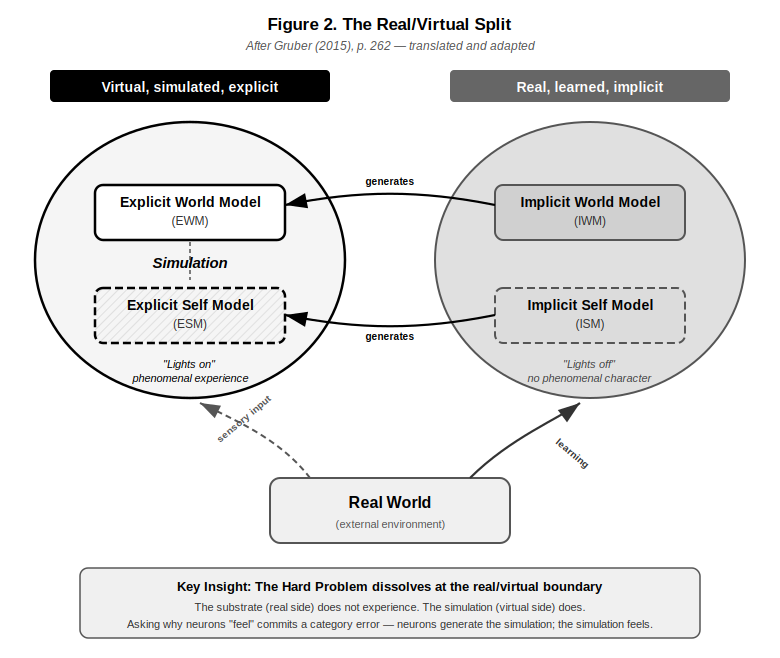
\includegraphics[width=0.95\textwidth]{../figures/figure2-real-virtual-split-bw.png}
  \caption{Die Real/Virtuell-Trennung. Das Substrat (reale Seite) speichert Wissen in synaptischen Gewichten -- physikalisch, strukturell, unbewusst. Die Simulation (virtuelle Seite) erzeugt Erfahrung in Echtzeit -- flüchtig, dynamisch, bewusst.}
\end{figure}


Schon einfache neuronale Netzwerke mit nur drei Schichten können lernen, ihre Eingabe zu modellieren -- zeigt man ihnen genug Beispiele, bauen sie interne Repräsentationen der Muster auf, denen sie begegnen. Das Gehirn macht genau das, aber in einem weitaus reicheren Maßstab. Es baut nicht ein Modell; es baut viele, die alles abdecken vom Sehfeld bis zur Position der Gliedmaßen, vom Klang einer Stimme bis zum Druck der Füße auf dem Boden. Diese Modelle umfassen sowohl die Welt außerhalb \textit{als auch} den eigenen Körper und verknüpfen alle verfügbaren sensorischen Eingaben zu kohärenten Repräsentationen.

Die Neurowissenschaft kennt diese Modelle seit über einem Jahrhundert. Im motorischen Kortex und im somatosensorischen Kortex ist der Körper buchstäblich als verzerrte Karte dargestellt -- Hände und Lippen grotesk vergrößert, weil sie mehr Nervenenden haben, Rumpf und Beine zu Splittern komprimiert. Diese kortikalen Karten, \textit{Homunculi} genannt, wurden erstmals von Wilder Penfield in den 1930er Jahren durch direkte elektrische Stimulation während Hirnoperationen kartiert. Sie sind nur die anschaulichsten Beispiele; das Gehirn unterhält ähnliche Karten und Modelle in seiner gesamten Architektur. (Siehe Anhang A für mehr zur kortikalen Organisation.)


\begin{figure}[htbp]
  \centering
  \includegraphics[width=0.95\textwidth]{../figures/book/homunculi.en.png}
  \caption{Penfields kortikaler Homunculus. Der somatosensorische Kortex widmet Händen, Lippen und Zunge dramatisch mehr Fläche als dem gesamten Rumpf -- eine verzerrte Körperkarte, die die Dichte der Nervenenden widerspiegelt, nicht die Größe der Körperteile.}
\end{figure}


Ich nenne diese die \textbf{impliziten Modelle}: das Implizite Weltmodell (IWM) und das Implizite Selbstmodell (ISM). Sie sind in der Struktur des Gehirns gespeichert -- in den Stärken synaptischer Verbindungen, der Architektur neuronaler Schaltkreise, dem akkumulierten Lernen eines Lebens. Sie sind die Festplatte des Gehirns. Sie werden nie direkt erfahren, nicht mehr als das Silizium im eigenen Handy. Aber sie kodieren alles, was das Gehirn über die Welt und über einen selbst weiß.

Nun die Schlüsseleinsicht. Diese impliziten Modelle sitzen nicht einfach nur da. Sie \textit{erzeugen} etwas. In der Technik ist ein \textbf{digitaler Zwilling} eine Echtzeit-virtuelle Replik eines physischen Systems (ein Düsentriebwerk, ein Stromnetz, eine Fabrikhalle), kontinuierlich aktualisiert mit Sensordaten, damit Ingenieure das System überwachen und mit ihm interagieren können, ohne es direkt zu berühren. Die impliziten Modelle tun genau das. Sie produzieren eine Echtzeit-virtuelle Simulation der Welt und eine Echtzeit-virtuelle Simulation von einem selbst. Das sind die \textbf{expliziten Modelle}: das Explizite Weltmodell (EWM) und das Explizite Selbstmodell (ESM). Alles, was man sieht, hört, fühlt und denkt, geschieht innerhalb dieser Simulationen, nicht in der Welt selbst.

Zwei Gruppen von Modellen (implizit und explizit), jede mit sowohl einem Weltmodell als auch einem Selbstmodell. Vier Modelle insgesamt, und mit ihnen eine Sprache, um darüber zu sprechen, was Bewusstsein tatsächlich tut. (Eine Anmerkung für Neurowissenschaftler und technisch versierte Leser: Die Zahl „vier\grqq{} ist ein prinzipielles Minimum, keine wörtliche Zählung dessen, was das Gehirn unterhält. Wer das beunruhigend findet, lese bitte Anhang E, bevor es weitergeht -- er adressiert dies direkt.)

Aber wo laufen diese Modelle? Das Gehirn nutzt mindestens fünf Ebenen der Informationsverarbeitung, aufeinander gestapelt. Die Simulation (die bewusste Erfahrung) läuft ganz oben.

\section*{Fünf verschachtelte Systeme}


\begin{figure}[htbp]
  \centering
  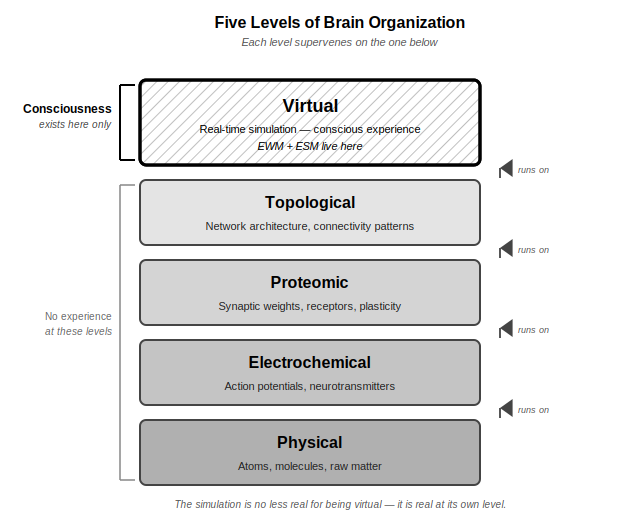
\includegraphics[width=0.95\textwidth]{../figures/figure-five-layer-stack-bw.png}
  \caption{Fünf Ebenen der Gehirnorganisation. Jede Ebene superveniert auf („läuft auf\grqq{}) der darunter liegenden. Bewusstsein existiert nur auf der obersten virtuellen Ebene, wo die expliziten Modelle phänomenale Erfahrung erzeugen.}
\end{figure}


Das Gehirn lässt sich als fünf verschiedene Organisationsebenen denken, gestapelt wie russische Puppen:

\textbf{Physikalisch.} Ganz unten die rohe Materie: Atome, Moleküle, das physische Substrat des Gehirns selbst. Das ist die Chemie -- der Kohlenstoff, Wasserstoff, Stickstoff, Sauerstoff, die das Gewebe bilden. Inerte Materie, die den Gesetzen der Thermodynamik gehorcht. Nichts Bewusstes lebt hier.

\textbf{Elektrochemisch.} Eine Ebene höher: neuronale Signalübertragung. Aktionspotenziale rasen Axone hinunter, Neurotransmitter überfluten Synapsen, Ionen fließen durch Kanäle. Das ist die elektrische und chemische Aktivität, die sich jeder vorstellt beim Gedanken „Gehirn tut etwas\grqq{}. Die Ebene, wo Neuronen feuern. Immer noch keine Erfahrung, aber jetzt gibt es Informationsübertragung.

\textbf{Proteomisch.} Als Nächstes: Proteinstrukturen und molekulare Maschinerie. Synaptische Gewichte werden hier gespeichert -- die physischen Stärken der Verbindungen zwischen Neuronen. Rezeptoren auf Zellmembranen, Enzyme, die Plastizität regulieren, das molekulare Gerüst, das bestimmt, welche Synapsen stärker werden und welche schwächer. Das ist die „Hardware\grqq{} des Lernens. Wer eine Fähigkeit übt und besser wird, verändert die proteomische Schicht. Immer noch unbewusst, aber jetzt gibt es Gedächtnis.

\textbf{Topologisch.} Noch höher: Netzwerkarchitektur. Die Muster der Konnektivität, welche Neuronen mit welchen verbunden sind, wie dicht, in welchen Konfigurationen. Hier leben Brodmann-Areale, hier leben kortikale Säulen, hier existiert die großräumige Struktur von „visueller Kortex spricht mit motorischem Kortex\grqq{}. Es ist der Schaltplan. Ändert man diese Ebene, ändert sich, welche Arten von Verarbeitung das System leisten kann. Hier werden die impliziten Modelle (das IWM und ISM) gespeichert. Immer noch unbewusst. Aber jetzt gibt es Wissen.

\textbf{Virtuell.} Ganz oben: die simulierte Welt. Der kortikale Automat -- das dynamische Muster elektrischer Aktivität, das über das Netzwerk tanzt, Informationen integriert, Vorhersagen generiert, die Modelle in Echtzeit laufen lässt. Hier lebt die bewusste Erfahrung. Die expliziten Modelle (das EWM und ESM) existieren hier und nur hier. Das ist die einzige Ebene, die sich nach etwas anfühlt.

Jede Ebene superveniert auf der darunter liegenden, hat aber ihre eigene Dynamik. Ohne physische Materie keine elektrochemische Signalübertragung, ohne Chemie keine Proteinstrukturen, ohne Synapsen keine Netzwerktopologie, und ohne ein Netzwerk keine Simulation, die darauf laufen könnte. Aber jede Ebene hat Eigenschaften, die die niedrigeren Ebenen nicht haben. Eine Synapse ist nicht „über\glqq{} irgendetwas -- sie ist nur eine Verbindung. Ein Netzwerk von Synapsen \textit{ist} über etwas: es repräsentiert ein Gesicht, ein Wort, eine Erinnerung. Und die Simulation, die auf diesem Netzwerk läuft? Da wird aus „über\grqq{} „Erfahrung\grqq{}.

Diese Fünf-Ebenen-Hierarchie löst ein Problem, das fast jeden stolpern lässt, der diese Theorie zum ersten Mal hört: „Wenn Bewusstsein virtuell ist, worauf läuft es?\glqq{} Die Antwort: Es läuft auf der topologischen Ebene (dem Netzwerk), die in der proteomischen Ebene (synaptische Gewichte) implementiert ist, die auf der elektrochemischen Ebene (neuronales Feuern) läuft, die in der physischen Ebene (Materie) existiert. Bewusstsein ist nicht weniger real, weil es virtuell ist -- es ist nur real \textit{auf einer anderen Ebene} als Neuronen real sind. Der Berg im Videospiel ist real auf der Spielebene, auch wenn er „nur\grqq{} Transistoren auf der Hardware-Ebene ist. Gleiches Prinzip.

Ich werde im Laufe des Buches auf diese Hierarchie zurückkommen, besonders wenn wir in Kapitel 6 über Psychedelika sprechen -- weil Drogen nicht alle fünf Ebenen gleich treffen. Einige zielen auf die elektrochemische Ebene (Veränderung der Neurotransmitter-Dynamik), einige zielen auf die proteomische Ebene (Veränderung der Rezeptorexpression), und die Effekte wellen sich auf vorhersagbare Weise zur virtuellen Ebene hoch. Die Hierarchie ist nicht nur konzeptuell. Sie ist mechanistisch real und leistet Erklärungsarbeit.

Nun zu den vier Modellen.

\textbf{Das Implizite Weltmodell (IWM)} ist alles, was man über die Welt weiß. Nicht, woran man gerade denkt -- alles, woran man \textit{denken könnte}. Die Gesetze der Physik (fallende Objekte fallen, das wissen wir). Das Layout der eigenen Wohnung (im Dunkeln lässt sich darin navigieren). Die Grammatik der Muttersprache (ein Satz lässt sich als grammatisch oder ungrammatisch beurteilen, ohne die Regeln zu kennen). Die Gesichter aller, die man jemals gekannt hat. Der Geschmack von Schokolade. Das Geräusch von Regen.

All dieses Wissen ist in den synaptischen Verbindungen des Gehirns gespeichert -- den Stärken der Verbindungen zwischen Neuronen. Es wurde über das ganze Leben durch Erfahrung und Lernen aufgebaut. Und es ist nie, niemals direkt bewusst. In die eigenen neuronalen Verbindungen lässt sich nicht introspizieren. Die eigenen Synapsen lassen sich nicht fühlen. Das Implizite Weltmodell ist wie eine riesige Bibliothek, die man nie betritt -- man liest nur die Bücher, die sie einem an den Schreibtisch schickt.

\textbf{Das Implizite Selbstmodell (ISM)} ist alles, was man über sich selbst weiß. Das Körperschema -- die unbewusste Repräsentation, wo die Gliedmaßen sind, wie groß sie sind, wie sie sich bewegen. Die motorischen Fähigkeiten (Fahrradfahren, Tippen, ein Instrument spielen). Die Persönlichkeitsmerkmale, sozialen Fähigkeiten, emotionalen Muster, Gewohnheiten. Die autobiographische Gedächtnisstruktur (das Gerüst, das die Erinnerungen zu einer Lebensgeschichte organisiert).

Wie das Weltmodell ist das Selbstmodell in synaptischen Gewichten gespeichert und nie direkt bewusst. Man erfährt nicht das Körperschema; man erfährt den Körper, den das Schema erzeugt. Man erfährt nicht die Persönlichkeit; man erfährt die Gedanken und Gefühle, die sie produziert. Das Implizite Selbstmodell ist die Hinterbühnen-Crew -- essenziell für die Aufführung, aber nie vom Publikum gesehen.

\textbf{Das Explizite Weltmodell (EWM)} ist die Welt, die man tatsächlich erfährt. Gerade jetzt. Der Raum, in dem man sich befindet, die Geräusche, die man hört, das Gewicht dieses Buches in den Händen (oder das Leuchten des Bildschirms, auf dem man es liest). Das ist die Simulation -- die Echtzeit-virtuelle Realität des Gehirns, erzeugt aus dem Impliziten Weltmodell plus aktueller sensorischer Eingabe. Sie ist lebendig, detailliert und nahtlos überzeugend. Man wird das ganze Leben darin leben und nie hinaustreten.

\textbf{Das Explizite Selbstmodell (ESM)} ist das \textit{Selbst}. Das Gefühl, ein Subjekt zu sein. Das Gefühl von „Ich\grqq{} -- derjenige, der sieht, hört, denkt und entscheidet. Auch das ist eine Simulation: ein Echtzeit-Modell, erzeugt aus dem Impliziten Selbstmodell plus aktuellen Körpersignalen. Es ist der Charakter, den das Gehirn erschafft, um seine virtuelle Welt zu bewohnen. Man IST der Charakter, den das Gehirn erschafft, um seine virtuelle Welt zu bewohnen.

\section*{Die reale Seite und die virtuelle Seite}


\begin{figure}[htbp]
  \centering
  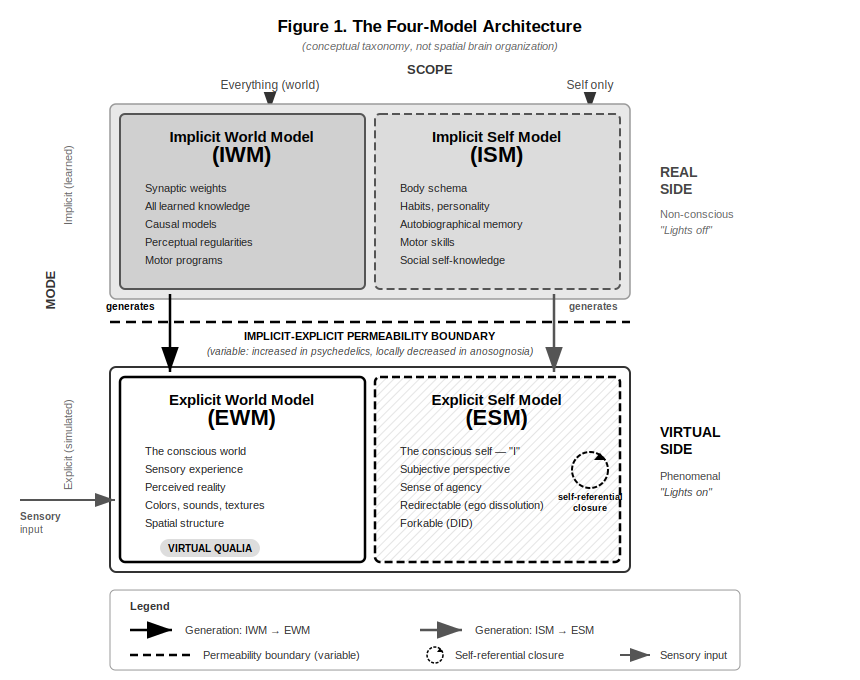
\includegraphics[width=0.95\textwidth]{../figures/figure1-four-model-architecture-bw.png}
  \caption{Die Vier-Modelle-Architektur. Das Gehirn unterhält zwei Arten von Modell (eines von der Welt, eines vom Selbst), jedes in zwei Modi: implizit (in der Struktur des Gehirns gespeichert) und explizit (aktiv laufend als Echtzeit-Simulation). Bewusstsein lebt in den expliziten Modellen.}
\end{figure}


Die vier Modelle teilen sich in zwei Seiten, und diese Teilung ist das Fundament von allem, was folgt.

Die \textbf{reale Seite} (die zwei impliziten Modelle) ist physikalisch, strukturell und relativ starr (durch Lernen angepasst). Es ist das gespeicherte Wissen des Gehirns: synaptische Gewichte, Netzwerkverbindungen, Rezeptorkonfigurationen. Man stelle es sich vor als alles, was das Gehirn \textit{gelernt hat} -- kristallisiert in die physische Struktur des Gewebes selbst. Es hat keine Erfahrung. Das Feuern einer Synapse wird nicht mehr „erfahren\grqq{} als Wasser, das durch ein Rohr fließt. Die reale Seite ist Licht aus.

Etwas, das es wert ist zu betonen: Die reale Seite ist das, was die Neurowissenschaft bereits studiert. Wenn ein Forscher jemanden in einen fMRT-Scanner steckt, schaut er auf die reale Seite -- Feuermuster, Konnektivität, Blutfluss zu verschiedenen Regionen. Wenn ein Neurochirurg einen kortikalen Bereich stimuliert und beobachtet, was passiert, sondiert er die reale Seite. Die Neurowissenschaft hat dieses Territorium seit über einem Jahrhundert kartiert, und sie hat außergewöhnliche Fortschritte gemacht. Die Vier-Modelle-Theorie weist keine dieser Arbeiten zurück. Sie sagt, dass all das nur die Hälfte des Bildes beschreibt.

Die \textbf{virtuelle Seite} (die zwei expliziten Modelle) ist simuliert, flüchtig und dynamisch. Sie wird in jedem Moment neu aus der realen Seite plus aktueller Eingabe erzeugt. Man stelle es sich vor als alles, was das Gehirn \textit{gerade mit} dem macht, was es gelernt hat -- die Live-Show, nicht das gespeicherte Skript. Und es ist \textit{alles} Erfahrung. Jeder Anblick, Klang, Gedanke, jedes Gefühl, jede Erinnerung, jeder Traum und jede Halluzination, die man jemals hatte, ist auf der virtuellen Seite aufgetreten. Die virtuelle Seite ist Licht an.

Aber hier ist der Haken: Die virtuelle Seite ist von außen unsichtbar. Selbst unsere fortschrittlichste Bildgebung des Gehirns kann sie nur indirekt erfassen. Ein fMRT zeigt, welche Hirnregionen aktiv sind -- das ist die reale Seite bei der Arbeit. Um tatsächlich bewusste Erfahrung aus Gehirndaten zu \textit{lesen}, müsste man die Programmiersprache des Gehirns entschlüsseln -- verstehen, nicht nur welche Neuronen feuern, sondern was das Muster des Feuerns \textit{bedeutet} auf der Simulationsebene. Das würde etwas wie ein vollständig simuliertes Konnektom erfordern: eine vollständige digitale Replik des Gehirns, in Software laufend, die dieselbe virtuelle Welt produziert, die das biologische Gehirn produziert.

Ich möchte ehrlich sein über das, was die Theorie gibt und nicht gibt. Die Vier-Modelle-Theorie sagt \textit{was} die Simulation ist, \textit{wo} sie lebt, und \textit{warum} sie sich nach etwas anfühlt. Sie händigt nicht den Entschlüsselungsring aus. Die virtuelle Seite aus der realen Seite zu lesen, ist ein zukünftiges Forschungsprogramm -- eines, das die Theorie klar definiert, aber noch nicht ausführen kann. Allerdings wird die Grundlage für dieses Programm bereits gelegt. Das Human Connectome Project und verwandte Bemühungen kartieren die Verdrahtung des Gehirns mit zunehmend feiner Auflösung. Die virtuelle Seite lässt sich noch nicht aus strukturellen Daten dekodieren, aber die strukturellen Daten kommen.

Wer wissenschaftlich denkt, sieht vielleicht schon, wohin das führt. Wenn Erfahrung nur auf der virtuellen Seite existiert, dann ist die Suche nach Erfahrung auf der realen Seite -- in den Neuronen, in den Synapsen, in der physischen Maschinerie -- an der völlig falschen Stelle. Es ist, als würde man nach der Handlung eines Films in den Schaltkreisen des DVD-Players suchen.

Das ist der Schlüssel. Hier ist er.

\section*{Wie bewusst ist man?}

Aber zuerst etwas, worüber man sich wahrscheinlich schon gewundert hat. Wenn Bewusstsein eine Simulation ist -- ein virtuelles Selbst innerhalb einer virtuellen Welt -- dann ist es keine Alles-oder-Nichts-Sache, oder? Eine Simulation kann mehr oder weniger detailliert sein. Ein Selbstmodell kann mehr oder weniger ausgereift sein. Das bedeutet, dass Bewusstsein in \textit{Graden} kommt.

Die Vier-Modelle-Theorie bietet eine präzise Möglichkeit, über diese Grade nachzudenken. Es gibt vier abgestufte Ebenen, und jedes bewusste Geschöpf sitzt irgendwo auf dieser Leiter.

Ganz unten steht \textbf{einfaches Bewusstsein}. Das ist ein Explizites Weltmodell mit nur einem rudimentären Expliziten Selbstmodell. Das System erzeugt eine virtuelle Welt -- es ist etwas wie etwas, dieses Geschöpf zu sein -- aber das Selbst innerhalb dieser Welt ist kaum skizziert. Man denke an eine Maus, die durch ein Labyrinth navigiert. Sie sieht die Wände, riecht den Käse, fühlt den Boden unter ihren Pfoten. Sie hat phänomenale Erfahrung. Aber ihr Modell von \textit{sich selbst} als das Ding, das diese Erfahrungen hat? Hauchdünn. Es gibt ein „wie es ist wie\glqq{}, aber fast kein „für wen es ist wie\grqq{}.

Eine Stufe höher: \textbf{einfach erweitertes Bewusstsein}. Jetzt wird das Selbstmodell real. Das System erfährt nicht nur -- es modelliert sich selbst \textit{als} den Erfahrenden. Es ist sich bewusst, dass es erfährt. Der Hund fühlt nicht nur Schmerz; er weiß, dass \textit{er} Schmerzen hat. Es gibt eine Ich-Perspektive -- ein echtes „Ich\grqq{} im Zentrum der virtuellen Welt. Das ist Selbstbeobachtung erster Ordnung, und es ändert alles. Leiden wird hier möglich, weil Leiden ein Selbst erfordert, das weiß, dass es leidet.

Dann: \textbf{doppelt erweitertes Bewusstsein}. Selbstbeobachtung zweiter Ordnung. Das System modelliert sich selbst, sich selbst zu modellieren. Das ist Metakognition -- Denken über das eigene Denken. Man liegt im Bett und fragt sich, ob die Angst vor dem morgigen Meeting rational ist oder ob man katastrophisiert. Die eigenen mentalen Zustände werden überwacht, bewertet, manchmal überschrieben. Hier lebt das meiste erwachsene menschliche Bewusstsein die meiste Zeit. Es ist die Ebene, die Therapie möglich macht, die es erlaubt zu sagen „Ich bemerke, dass ich wütend werde\grqq{} anstatt nur wütend zu sein.

Und ganz oben: \textbf{dreifach erweitertes Bewusstsein}. Dritte Ordnung. Das System modelliert sich selbst, sich selbst zu modellieren, sich selbst zu modellieren. Das klingt wie ein Spiegelsaal, und das ist es auch, aber es ist ein Spiegelsaal, den es braucht, um Philosophie des Geistes zu betreiben. Um zu fragen „was ist Bewusstsein?\grqq{} muss man sich selbst modellieren, die eigene Erfahrung modellieren und dann sich selbst modellieren, wie man diese Erfahrung modelliert. Es gilt, weit genug zurückzutreten, um den gesamten Apparat von außen zu sehen, obwohl man immer noch darin ist. Das ist die Voraussetzung für die Frage, die dieses Buch zu beantworten versucht. Nur Geschöpfe, die zu dreifach erweitertem Bewusstsein fähig sind, können sich fragen, warum irgendetwas sich nach irgendetwas anfühlt.

Die Auszahlung: Dieser Gradient ist nicht nur abstrakte Philosophie. Er beantwortet die Frage, die bei jeder Dinnerparty gestellt wird -- „Ist mein Hund bewusst?\grqq{} Die Antwort ist ja, aber weniger bewusst als wir selbst. Der Hund ist wahrscheinlich auf der einfach erweiterten Ebene. Er hat ein Selbst. Er hat Erfahrung. Er liegt nicht um 3 Uhr morgens wach und hinterfragt die Natur dieser Erfahrung. Wir werden in Kapitel 10 im Detail auf die Tierfrage zurückkommen, wo dieser Gradient echte Erklärungsarbeit leistet. Aber die Form davon ist schon erkennbar: Bewusstsein ist kein Lichtschalter. Es ist ein Dimmer.

\begin{figure}[htbp]
  \centering
  \includegraphics[width=0.95\textwidth]{../figures/figure3-phenomenological-content-bw.png}
  \caption{Phänomenologischer Gehalt im Tagesverlauf. Routinetätigkeiten führen zu niedrigem phänomenologischem Gehalt (Autopilot). Auffällige Ereignisse (Bedrohungen, soziale Signale) erzeugen hohen Gehalt. Bewusstsein verfolgt, was wichtig ist, nicht alles.}
  \label{fig:phenomenological}
\end{figure}



\section*{Warum das Gehirn die Fähigkeit zur Selbstmodellierung hat}

Also haben wir festgestellt, dass Bewusstsein von diesen vier Modellen abhängt, wobei das explizite Selbstmodell die Hauptlast trägt. Aber warum hat das menschliche Gehirn diese Fähigkeit überhaupt, wenn einfachere Tiere sie nicht haben? Die Antwort verbirgt sich in Sichtweite: Die Architektur des menschlichen Kortex ist buchstäblich überdimensioniert für grundlegende Informationsverarbeitung.

Der menschliche Neokortex hat sechs Schichten. Das ist eine wohlbekannte anatomische Tatsache, nachzulesen in jedem Neurobiologie-Lehrbuch. Aber hier ist, was interessant ist: Sechs Schichten braucht es nicht, um Informationen zu verarbeiten. Drei Schichten reichen aus.

Man überlege, was ein standardmäßiges neuronales Netzwerk leisten muss. Erste Schicht: Eingabe empfangen, filtern, aufräumen. Zweite Schicht: Muster extrahieren, Merkmale erkennen, die schwere Rechenlast heben. Dritte Schicht: Ergebnisse integrieren, Entscheidungen treffen, Ausgabe produzieren. Eingabe, Verarbeitung, Ausgabe. Das ist das Grundrezept, und drei Schichten decken es ab.

Aber wir haben sechs.

Wofür sind die „extra\grqq{} drei Schichten?

Sie sind dafür da, die ersten drei zu modellieren.

Ein Drei-Schichten-Netzwerk verarbeitet die Welt. Ein Sechs-Schichten-Netzwerk verarbeitet die Welt \textit{und} beobachtet sich dabei selbst. Die zusätzlichen Schichten bieten die architektonische Kapazität für das Gehirn, nicht nur ein Modell dessen zu bauen, was da draußen ist, sondern ein Modell von sich selbst, wie es modelliert, was da draußen ist. Selbstsimulation erfordert diese Verdopplung -- es braucht einen Satz von Schichten, um die Verarbeitung zu tun, und einen anderen Satz, um die Verarbeitung geschehen zu sehen.

Das ist keine Spekulation darüber, was einzelne Schichten „tun\glqq{} -- ich behaupte nicht, dass Schicht 4 dies tut und Schicht 5 das tut. Es ist eine Beobachtung über architektonische Kapazität. Sechs Schichten geben Raum für sowohl das implizite Weltmodell (die gelernte, unbewusste Verarbeitung) als auch das explizite Weltmodell (die Echtzeit-Simulation). Sie geben Raum für sowohl das implizite Selbstmodell (Körperschema, Motorprogramme, Persönlichkeitsstruktur) als auch das explizite Selbstmodell (das „Ich\grqq{}, das erlebt, einen Körper zu haben, Handlungen zu initiieren, eine Person zu sein).

Nun schaue man auf andere Tiere. Reptilien haben drei oder vier kortikale Schichten. Säugetiere haben sechs. Und unter den Säugetieren sind diejenigen mit dem dicksten, am aufwendigsten gefalteten Kortex (Primaten, Wale, Elefanten) genau diejenigen, die die reichsten Anzeichen von Selbstbewusstsein zeigen. Selbsterkennung im Spiegel, Zukunftsplanung, soziale Täuschung, Trauer. Die architektonische Kapazität verfolgt die Phänomenologie.

Der Sprung von drei auf sechs Schichten könnte ein genetischer Duplikationsunfall gewesen sein -- Evolutions-Copy-Paste, das genau die Architektur produzierte, die Bewusstsein später ausnutzen würde. Reptilien-Vorfahren hatten drei kortikale Schichten. Irgendwo im Übergang zu Säugetieren verdoppelte sich diese Zahl. Die Transkriptionsfaktoren, die kortikale Schichtidentität spezifizieren (Tbr1, Satb2, Ctip2, Fezf2), haben Paraloge, die auf Genduplikationsereignisse hinweisen. Ob das ein einzelnes dramatisches Ereignis war oder eine allmähliche Ausarbeitung, bleibt umstritten, aber das Ergebnis ist klar: Säugetiere bekamen das Doppelte an Schichten, und mit ihnen die Fähigkeit zur Selbstmodellierung, die den meisten Reptilien fehlt.

Das ist die Brücke von der neuronalen Netzwerktheorie zur gelebten Erfahrung. Der menschliche Kortex ist nicht nur ein großer Mustererkenner. Es ist ein überdimensioniertes, rekursiv strukturiertes Netzwerk mit genug Schichten, um seinen eigenen Modellierungsprozess zu modellieren. Und wenn ein Netzwerk sich selbst modelliert, wie es die Welt modelliert, ist das Ergebnis -- von innen betrachtet -- genau das, was wir Bewusstsein nennen.

Ich sollte klarstellen: Ich behaupte nicht, dass sechs kortikale Schichten die \textit{einzige} Architektur sind, die Bewusstsein unterstützen kann. Sie sind eine Lösung -- die, die Säugetiere entwickelt haben. Aber es könnte andere geben. Der Oktopus, mit seinem radikal verteilten Nervensystem (acht semi-autonome Arme, jeder mit seinem eigenen neuronalen Verarbeitungszentrum, das etwa 40 Millionen Neuronen enthält), repräsentiert einen völlig anderen architektonischen Ansatz, der möglicherweise äquivalente Rechenleistung erreicht. Vögel bieten ein weiteres markantes Beispiel: Rabenvögel und Papageien fehlt ein geschichteter Kortex völlig, ihr Pallium ist in Kerncluster organisiert statt in Schichten, dennoch machen Krähen Werkzeuge, planen für die Zukunft und erkennen sich wohl im Spiegel. Worauf es ankommt, ist die Fähigkeit zur Selbstmodellierung, nicht der spezifische Schaltplan -- jede Architektur, die eine Simulation von sich selbst laufen lassen kann, könnte im Prinzip bewusst sein. Wir werden in Kapitel 10 darauf zurückkommen.

\chapter{Die virtuelle Seite}

Stellen wir uns vor, wir spielen ein Videospiel. Ein gutes --- ein immersives Open-World-Spiel mit atemberaubender Grafik, realistischer Physik und einer fesselnden Geschichte. Man steuert eine Figur und interagiert durch diese Figur mit einer detailreich gestalteten virtuellen Welt.

Nun überlege man: Wo existiert das Spiel? Nicht auf dem Bildschirm, genau genommen --- der Bildschirm zeigt nur Lichtmuster. Nicht in der Grafikkarte oder der CPU, genau genommen --- diese leiten elektrische Signale durch Siliziumschaltkreise. Das Spiel existiert als ein \textit{virtueller Prozess} --- ein höherstufiges Phänomen, das aus der Aktivität der Hardware hervorgeht, aber nicht mit irgendeinem bestimmten Stück Hardware identisch ist.

Die virtuelle Welt des Spiels hat Eigenschaften, die die Hardware nicht hat. Das Spiel hat Berge, Flüsse und Städte. Die CPU hat Transistoren. Das Spiel hat einen Tag-Nacht-Zyklus. Die GPU hat Taktzyklen. Es lässt sich sinnvoll fragen „Wie hoch ist dieser Berg im Spiel?\glqq{}, aber es wäre absurd, auf einen Transistor zu zeigen und zu sagen „Dieser Transistor ist 3.000 Meter hoch.\grqq{} Die Eigenschaften des Spiels existieren auf der virtuellen Ebene, und sie sind echte Eigenschaften des Spiels, auch wenn das Spiel „nur\grqq{} ein Aktivitätsmuster in der Hardware ist.

Das ist keine Metapher. So funktioniert das Gehirn.

Das Explizite Weltmodell (EWM) --- die Welt, die man erlebt --- ist ein virtueller Prozess, der auf neuronaler Hardware läuft, genauso wie die Spielwelt ein virtueller Prozess ist, der auf Silizium-Hardware läuft. Die erlebte Welt hat Eigenschaften (Farben, Formen, Entfernungen, Klänge), die die neuronale Hardware nicht hat (die Hardware hat Feuerraten, synaptische Stärken und Neurotransmitter-Konzentrationen). Die Eigenschaften der erlebten Welt sind \textit{echte Eigenschaften der Simulation}, auch wenn die Simulation „nur\grqq{} ein Muster neuronaler Aktivität ist.

Das Explizite Selbstmodell (ESM) --- das „Ich\grqq{}, das die Welt erlebt --- ist ebenfalls ein virtueller Prozess. Es ist so real wie die Spielfigur in der Analogie: echt existierend auf der virtuellen Ebene, wirklich Eigenschaften besitzend auf der virtuellen Ebene, aber nicht existierend auf der Hardware-Ebene.

\section*{Warum die Analogie zusammenbricht (auf die wichtige Art)}

Die Videospiel-Analogie ist nützlich, aber sie bricht an einem entscheidenden Punkt zusammen: Das Spiel hat einen \textit{Spieler}. Es gibt jemanden außerhalb des Spiels --- auf der Couch sitzend --- der das Spiel erlebt. Das Spiel selbst hat keine Erfahrung. Es sind nur Lichtmuster und Code.

Die Simulation des Gehirns hat keinen externen Spieler. Niemand sitzt außerhalb des Schädels und erlebt die Simulation. Die Simulation enthält ihren eigenen Beobachter --- das Explizite Selbstmodell. Die Simulation \textit{ist} die Erfahrung, nicht etwas, das von jemand anderem erfahren wird.

Versetzen wir uns in die Position der Spielfigur. Man \textit{ist} die Hauptfigur. Von außerhalb des Spiels sieht ein Zuschauer Pixel, die sich auf einem Bildschirm bewegen --- nichts, das möglicherweise etwas fühlen könnte. Aber von innerhalb der Simulation? Die Spielwelt ist alles, was es gibt. Die Berge sind real für die Figur, das Sonnenlicht ist warm, die Gefahr ist beängstigend. Kein externer Beobachter würde je vermuten, dass dieser Haufen Code etwas fühlt, aber das liegt daran, dass sie auf die falsche Ebene schauen. Sie schauen auf die Hardware. Die Erfahrung existiert auf der Software-Ebene. Das ist meine Behauptung, und der Rest dieses Buches legt die Beweise dar.

[ABBILDUNG: SDXL/Flux --- \glqq{}Ego-Perspektive aus dem Inneren einer fotorealistischen virtuellen Welt, Blick auf eine lebhafte, sonnenbeschienene Landschaft mit Bergen und einem Fluss. An den Rändern des Sichtfelds löst sich die fotorealistische Szene auf und fragmentiert in leuchtende neuronale Netzwerke, synaptische Verbindungen, fließende elektrische Impulse und durchscheinende schaltkreisähnliche Muster. Der Übergang von lebhafter Realität zum neuronalen Substrat (Substrat) ist graduell und organisch und zeigt, dass die Welt und der Beobachter aus demselben gemacht sind. Volumetrisches Licht, Tiefenschärfe, kinematografische Komposition, Konzeptkunst, digitales Gemälde, 8k, hochdetailliert\grqq{} --- Negativ: \glqq{}text, watermark, signature, blurry, low quality, cartoon, anime, extra fingers, deformed, ugly, duplicate, out of frame\grqq{} --- Landscape 16:9, CFG 7-8, steps 30-40. Bei Flux: negatives Prompt weglassen.]

\textit{Die Simulation betrachtet sich selbst. Das gesamte Sichtfeld --- jede Farbe, Form und Schatten --- wird vom Echtzeit-Virtualmodell des Gehirns generiert. An den Rändern wird die Illusion dünner und die neuronale Maschinerie wird sichtbar. Es gibt keine Grenze zwischen dem Beobachter und dem Beobachteten. Man ist die Simulation.}

Das ist es, was Bewusstsein besonders macht und was das Schwierige Problem (Hard Problem) so unlösbar erscheinen lässt. Im Videospiel gibt es eine klare Trennung zwischen dem Spiel (virtuell, keine Erfahrung) und dem Spieler (physisch, hat Erfahrung). Im Gehirn gibt es keine Trennung. Die Simulation und der Erfahrende sind dasselbe. Das Explizite Selbstmodell beobachtet nicht das Explizite Weltmodell von außen --- es ist \textit{innerhalb} der Simulation, Teil desselben virtuellen Prozesses.

Und dieser selbstreferentielle Abschluss (die Simulation beobachtet sich selbst von innen) ist, so argumentiere ich, was wir Bewusstsein nennen. Es ist nicht etwas, das zur Simulation hinzugefügt wird. Es ist das, was die Simulation \textit{ist}, wenn sie ein Modell von sich selbst enthält. Deshalb sage ich, Bewusstsein ist kein Ding --- es ist ein Prozess. Man wird es nicht finden, indem man das Gehirn auseinandernimmt, genauso wenig wie man ein laufendes Programm findet, indem man die CPU zerlegt.

\section*{Die Software-Eigenschaften}

Wenn die virtuellen Modelle wirklich software-ähnliche Prozesse sind, die auf neuronaler Hardware laufen, dann sollten sie sich auf spezifische, testbare Weisen wie Software verhalten. Und das tun sie. Vier Eigenschaften der virtuellen Seite werden in diesem Buch immer wieder auftauchen, also seien sie hier dargelegt.

\textbf{Forking (Aufspaltung).} Ein einzelnes Substrat kann mehrere virtuelle Konfigurationen gleichzeitig laufen lassen. In Software forkt man einen Prozess und erhält zwei unabhängige Instanzen, die auf derselben Hardware laufen. Im Gehirn ist dies die Dissoziative Identitätsstörung --- mehrere Selbstmodelle, jedes mit seiner eigenen Erzählung und emotionalem Profil, die abwechselnd die Kontrolle über dasselbe neuronale Substrat übernehmen. Wir werden das in Kapitel 9 sehen.

\textbf{Cloning (Klonen).} Trenne die Hardware physisch, und du erhältst degradierte, aber vollständige Kopien der Software. Schneide das Corpus callosum durch, und jede Hemisphäre läuft ihre eigene Version der Simulation --- weniger leistungsfähig als das Original, aber funktional vollständig. Das ist das Split-Brain-Phänomen, ebenfalls Kapitel 9.

\textbf{Redirecting (Umleiten).} Unterbreche den normalen Input-Strom und die Simulation klinkt sich in welches Signal auch immer dominant ist. Unter Salvia divinorum überwältigt propriozeptiver Input das System und das Explizite Selbstmodell rekonfiguriert sich um Körperempfindung herum. Unter Ketamin fällt externer Input aus und die Simulation läuft auf internem Rauschen. Die virtuellen Modelle stoppen nicht --- sie verarbeiten nur, was immer ihnen zugeführt wird. Kapitel 6 behandelt dies im Detail.

\textbf{Reconfiguring (Neukonfiguration).} Verändert man die Verbindungsgewichte des Substrats, ändert sich, was die virtuellen Modelle produzieren. Genau das tut Kognitive Verhaltenstherapie --- systematisches Neuverkabeln des Substrats, sodass das Explizite Selbstmodell andere Erzählungen, andere emotionale Reaktionen, anderes Verhalten generiert.

Die Vier-Modelle-Theorie (VMT) macht eine spezifische Vorhersage über Therapie: Jede wirksame Behandlung muss funktionieren, indem sie die impliziten Modelle (das Substrat) so modifiziert, dass sich die expliziten Modelle (die Simulation) entsprechend verändern. Kognitive Verhaltenstherapie tut genau das. Sie identifiziert systematisch fehlangepasste Muster im ISM und verkabelt sie durch strukturierte Übung neu, wodurch sich ändert, was das ESM produziert. Deshalb hat Kognitive Verhaltenstherapie die stärkste Evidenzbasis aller Psychotherapien: Sie zielt auf die richtige Ebene ab.

Das wirft eine unbequeme Frage auf bezüglich Therapien, die ihren Mechanismus nicht in diesen Begriffen erklären können. Wenn ein therapeutischer Ansatz nicht spezifiziert, was er im Substrat verändert oder wie diese Veränderung zur Simulation propagiert, dann funktioniert er bestenfalls über einen Mechanismus, den er nicht versteht, und schlimmstenfalls funktioniert er überhaupt nicht. Die Evidenz bestätigt dies: Die Therapien mit den schwächsten Evidenzbasen sind generell jene mit den vagsten Theorien der Veränderung. Wer Therapie sucht, sollte dem Therapeuten eine einfache Frage stellen: „Was genau versuchen Sie in meinem Gehirn zu verändern, und wie?\grqq{} Wer darauf keine Antwort bekommt, sollte sich überlegen, jemanden zu finden, der eine hat.

Das sind keine Metaphern. Das sind strukturelle Vorhersagen. Wenn meine Theorie falsch ist und die virtuellen Modelle \textit{nicht} software-ähnliche Prozesse sind, dann sind diese Parallelen reiner Zufall. Aber Zufälle reihen sich normalerweise nicht vier-für-vier über klinische Neurologie, Psychopharmakologie und Psychotherapie hinweg auf. Die folgenden Kapitel werden jede Eigenschaft in Aktion zeigen.

Es gibt ein einfaches Experiment, das sich jetzt sofort durchführen lässt --- nun ja, mit einem Freund, einer Gummihand, einem Kartonschirm und zwei Pinseln --- und das demonstriert, wie leicht das Explizite Selbstmodell getäuscht werden kann. Es ist die Gummihand-Illusion, entwickelt von Matthew Botvinick und Jonathan Cohen, und sie ist einer der aufschlussreichsten Party-Tricks in der gesamten Neurowissenschaft.

Der Aufbau ist einfach. Man sitzt an einem Tisch mit einem Arm hinter einem Kartonschirm versteckt. Eine realistische Gummihand wird sichtbar platziert, ungefähr dort, wo die versteckte Hand wäre. Jemand streicht gleichzeitig über die Gummihand und die versteckte echte Hand mit zwei Pinseln, an derselben Stelle, mit derselben Geschwindigkeit. Nach ein oder zwei Minuten dieses synchronisierten Streichens passiert etwas Unheimliches: Man beginnt \textit{zu fühlen}, wie der Pinsel über die Gummihand streicht. Nicht über die echte Hand, hinter dem Schirm. Über die falsche Hand vor den eigenen Augen.

Das Explizite Selbstmodell hat die Gummihand in das Körperschema integriert. Es hat die Eigentümerschaft neu zugewiesen --- entschieden, dass die Gummihand Teil von „einem selbst\glqq{} ist. Das Selbstmodell ist nicht festverdrahtet. Es ist gelernt. Es wird kontinuierlich auf Basis der besten verfügbaren Evidenz aktualisiert, und wenn die visuelle Evidenz (sehen, wie die Gummihand gestrichen wird) konsistent mit der taktilen Evidenz übereinstimmt (fühlen, wie die echte Hand gestrichen wird), zieht das ESM die rationale Schlussfolgerung: Diese Hand ist meine. Wenn jemand dann die Gummihand bedroht (einen Hammer darauf niedergehen lässt), zuckt man zusammen, fühlt einen Angstschub, die galvanische Hautreaktion schießt hoch. Für den Teil des Gehirns, der das „Ich\grqq{} definiert, \textit{ist} diese Hand die eigene.

Das ist kein Fehler. Das ist das Selbstmodell, das genau so funktioniert, wie es entworfen ist --- ständig seine Körpergrenze auf Basis multimodaler sensorischer Korrelation aktualisierend. Es ist derselbe Mechanismus, der es Amputierten erlaubt, ein prothetisches Glied nach einer Nutzungsperiode als ihr eigenes zu „fühlen\grqq{}. Und es ist derselbe Mechanismus, der bei Asomatognosie zusammenbricht, wo Patienten die Eigentümerschaft ihrer tatsächlichen Gliedmaßen leugnen, und beim Alien-Hand-Syndrom, wo die Hand sich von selbst bewegt.

\section*{Das Patchwork-Hologramm}

Es gibt eine fünfte Eigenschaft der virtuellen Seite, die ihren eigenen Abschnitt verdient, weil sie etwas erklärt, das Neurowissenschaftler seit fast einem Jahrhundert verwirrt hat: warum Hirnschädigung Funktionen \textit{graduell} verschlechtert, anstatt spezifische Erinnerungen zu löschen.

In den 1920er und 30er Jahren trainierte der Psychologe Karl Lashley Ratten, ein Labyrinth zu navigieren, und entfernte dann chirurgisch Stücke ihres Kortex, um herauszufinden, wo die Erinnerung gespeichert war. Er fand sie nie. Egal welches Stück er entfernte, die Ratten erinnerten sich noch an das Labyrinth. Was zählte, war \textit{wie viel} Kortex er entfernte, nicht \textit{welche Teile}. Entfernte er ein wenig, wurden die Ratten etwas schlechter. Entfernte er viel, wurden sie viel schlechter. Aber die Erinnerung war nie einfach \textit{weg}, sauber herausgeschnitten wie eine Datei, die von einer Festplatte gelöscht wurde. Lashley verbrachte seine Karriere damit, das „Engramm\grqq{} zu suchen --- die physische Spur einer Erinnerung --- und kam berühmterweise zu dem Schluss, dass es nicht zu existieren schien.

Er suchte nach der falschen Sache. Die Erinnerung war nicht \textit{in} einem bestimmten Stück Kortex gespeichert, so wie eine Datei auf einem bestimmten Sektor einer Festplatte gespeichert ist. Sie war \textit{über} das gesamte Netzwerk verteilt, in den Verbindungsgewichten zwischen Millionen von Neuronen. So funktionieren neuronale Netzwerke: Information sitzt nicht in irgendeinem einzelnen Knoten. Sie ist im Muster der Verbindungen zwischen allen von ihnen kodiert. Man kann nicht auf eine einzelne Synapse zeigen und sagen „hier ist das Labyrinth gespeichert\glqq{}, genauso wenig wie man auf ein einzelnes Pixel zeigen und sagen kann „hier ist der Film gespeichert.\grqq{}

Das ist im Wesentlichen eine holografische Eigenschaft. Nimmt man ein physisches Hologramm und halbiert es, erhält man nicht zwei Hälften des Bildes. Man erhält zwei Kopien des \textit{vollständigen} Bildes, jede in niedrigerer Auflösung. Schneidet man es in Viertel, erhält man vier vollständige Bilder, noch verschwommener. Die Information in einem Hologramm ist über die gesamte Platte verteilt, sodass jedes Stück das ganze Bild enthält --- nur mit weniger Detail.

Neuronale Netzwerke tun dasselbe. Trainiert man ein Netzwerk, Gesichter zu erkennen, und zerstört dann 10\% seiner Verbindungen zufällig, vergisst es nicht 10\% der Gesichter. Es wird etwas schlechter bei \textit{allen} Gesichtern. Zerstört man 50\%, wird es substanziell schlechter bei allem, erkennt aber immer noch etwas. Die Information ist über das gesamte Netzwerk verschmiert, was genau der Grund ist, warum Lashley das Engramm nicht finden konnte: Es war überall und nirgends.

Aber --- und hier wird es interessant --- das Gehirn ist \textit{nicht} ein Hologramm. Es ist das, was ich ein \textit{Patchwork-Hologramm} nenne. Innerhalb eines einzelnen funktionalen Areals (sagen wir, dem primären visuellen Kortex, ungefähr Brodmann-Areal 17) sind die kortikalen Säulen einander ähnlich, und Information wird holografisch gespeichert. Zerstört man ein paar Säulen, fällt es kaum auf. Das Areal ist lokal holografisch (ein Teil enthält das Ganze, in niedrigerer Auflösung).

Auf der globalen Ebene tun verschiedene Areale verschiedene Dinge. Der visuelle Kortex ist nicht austauschbar mit dem motorischen Kortex. Entfernt man den gesamten visuellen Kortex, verliert man das Sehen --- es gibt kein verschwommenes Backup. Also ist das Gehirn lokal holografisch innerhalb jeder funktionalen Region, fraktal selbstähnlich in seiner kolumnaren Architektur, aber global \textit{nicht} holografisch. Es ist ein Patchwork: Dutzende holografische Kacheln, zusammengenäht zu einem Kompositum, das als Ganzes entschieden nicht-holografisch ist.

Diese Patchwork-Struktur erklärt ein Muster, das in der klinischen Neurologie immer wieder auftaucht. Kleine Schlaganfälle und kleine Läsionen verursachen oft überraschend milde Defizite, weil innerhalb eines gegebenen kortikalen Areals das holografische Prinzip schützt. Das verbleibende Gewebe rekonstruiert die fehlende Information in niedrigerer Auflösung. Aber große Schlaganfälle, die ein gesamtes funktionales Areal auslöschen, verursachen katastrophale, spezifische Verluste (Blindheit, Lähmung, Aphasie), weil eine ganze Kachel aus dem Patchwork entfernt wurde und keine andere Kachel substituieren kann.

Es erklärt auch, warum Erinnerungen nicht einfach „aus der Existenz springen\grqq{}, wenn Neuronen sterben. Jeden Tag sterben Neuronen und Synapsen werden beschnitten. Wenn Erinnerungen wie Dateien auf einer Festplatte gespeichert wären, würde man erwarten, gelegentlich eine zu verlieren --- eines Morgens aufzuwachen und die eigene Hochzeit vergessen zu haben, oder den Kindheitshund, oder den Geschmack von Kaffee. Das passiert nie. Stattdessen verblassen Erinnerungen allmählich, verlieren über Jahre Detail und Lebhaftigkeit. Das ist genau das, was ein holografisches Speichersystem vorhersagt: Degradation ist anmutig, proportional und global, niemals plötzlich, diskret oder lokal.

Das Patchwork-Hologramm ist der physische Grund, warum die Software-Eigenschaften, die ich oben beschrieben habe (besonders das Klonen) tatsächlich funktionieren. Teilt man das Gehirn in zwei Hälften, behält jede Hälfte eine degradierte, aber vollständige Kopie der Simulation, weil innerhalb jeder Hemisphäre das holografische Prinzip sicherstellt, dass jedes Stück das ganze Bild enthält. Die Simulation bricht nicht zusammen. Sie läuft nur in niedrigerer Auflösung.

\chapter{Warum es sich wie etwas anfühlt (und warum das die falsche Frage ist)}

Jetzt können wir uns dem Schwierigen Problem direkt stellen.

Die Frage ist: \textbf{Warum fühlt sich physische Verarbeitung wie etwas an?}

Die Antwort: \textbf{Tut sie nicht.}

Die physische Verarbeitung (Neuronen feuern, Synapsen übertragen, die impliziten Modelle speichern und berechnen) hat keine Erfahrung. Keine. Es gibt nichts, wie es ist, die reale Seite zu sein. Die reale Seite ist genau die \glqq{}im Dunkeln\grqq{}-Verarbeitung, von der das Schwierige Problem annimmt, dass Bewusstsein sie erklären muss.

Die \textit{Simulation} fühlt. Das Explizite Weltmodell und das Explizite Selbstmodell (die virtuelle Seite) sind der Ort, an dem Erfahrung lebt. Und innerhalb der Simulation ist Erfahrung keine mysteriöse Addition zum Prozess. Erfahrung ist das, was die Simulation \textit{ist}, wenn sie ein Selbstmodell enthält. Das Explizite Selbstmodell, das das Explizite Weltmodell \glqq{}wahrnimmt\grqq{}, ist das, was wir Qualia nennen. Qualia sind die Art und Weise des virtuellen Selbst, die virtuelle Welt zu registrieren.

Stellen wir uns das so vor: Wenn jemand fragen würde \glqq{}Warum fühlt sich das Schalten von Transistoren wie ein laufendes Videospiel an?\grqq{}, wäre die Antwort: \glqq{}Tut es nicht. Das Schalten von Transistoren fühlt sich nach gar nichts an. Das Spiel ist ein virtueller Prozess, der auf Transistoren läuft, aber Eigenschaften hat, die die Transistoren nicht haben --- Landschaften und Charaktere und Physik und Licht. Diese Eigenschaften sind echte Eigenschaften des virtuellen Prozesses, nicht der Transistoren.\grqq{}

Ähnlich: Neuronales Feuern fühlt sich nicht wie Rot-Sehen an. Neuronales Feuern generiert und erhält eine Simulation aufrecht, und innerhalb dieser Simulation nimmt das Selbstmodell eine bestimmte Klasse von Weltmodell-Inhalt als das wahr, was wir \glqq{}Röte\grqq{} nennen. Röte ist eine echte Eigenschaft der Simulation, keine Eigenschaft der Neuronen.

Das Schwierige Problem nahm an, dass wir erklären müssen, wie physische Verarbeitung Erfahrung produziert. Aber physische Verarbeitung produziert keine Erfahrung --- sie produziert eine \textit{Simulation}. Und die Simulation ist, weil sie eine selbstreferentielle Schleife enthält (das ESM modelliert sich selbst innerhalb des EWM), konstitutiv Erfahrung.

\section*{Die Zirkularitätsfrage}

Die erste Frage, die die meisten Leser stellen: \glqq{}Wurde das Problem nicht nur verschoben? Warum hat \textit{diese} Simulation Erfahrung, wenn eine Wettersimulation keine hat?\grqq{}

Die Antwort ist Selbstreferenz. Eine Wettersimulation modelliert Wetter. Sie modelliert nicht \textit{sich selbst}. Es gibt ein \glqq{}Außen\grqq{} zu einer Wettersimulation --- den Computer, den Programmierer, den Wissenschaftler, der die Ausgabe interpretiert. Die Simulation kann vollständig beschrieben werden, ohne auf irgendeine Erfahrung zu verweisen, weil es kein Selbstmodell in ihr gibt.

Die Simulation des Gehirns modelliert sich selbst. Das Explizite Selbstmodell ist das Modell der Simulation von \textit{ihrem eigenen Prozess}. Das erzeugt eine geschlossene Schleife: Das Modell und das Modellierte sind dasselbe System. Es gibt kein \glqq{}Außen\grqq{}, von dem aus die Simulation vollständig beschrieben werden kann, weil der Beschreibende Teil der Beschreibung ist.

Das ist keine Magie. Das ist eine strukturelle Konsequenz von Selbstreferenz. Wenn ein Prozess sich selbst modelliert, kollabiert die Unterscheidung zwischen Modell und Modelliertem. Der Prozess der Selbstmodellierung und die Erfahrung, ein Selbst zu sein, sind nicht zwei verschiedene Dinge, die durch eine Brücke verbunden werden müssen --- sie sind ein und dasselbe, beschrieben in verschiedenen Vokabularen.

Das Schwierige Problem fragt nach einer Brücke zwischen physischer Verarbeitung und Erfahrung. Die Vier-Modelle-Theorie sagt: Es gibt keine Brücke, weil sie nie getrennt waren. Die Erfahrung IST die Selbst-Simulation, aus dem Inneren der Schleife betrachtet.

Das ist letztlich eine Identitätsaussage (die Art von Aussage, die in der Wissenschaft einen Ruhepunkt markiert statt einer Lücke). \glqq{}Wasser ist H$_2$O\grqq{} ist eine Identität. Die Frage \glqq{}Aber \textit{warum} ist Wasser H$_2$O?\grqq{} ist nicht sinnvoll stellbar --- die Identität \textit{ist} die Erklärung. Nach etwas Tieferem zu fragen bedeutet, nach einer anderen Art von Universum zu fragen. Ähnlich: Erfahrung ist das, was Vier-Modell-Selbstsimulation bei Kritikalität (Criticality) \textit{ist}. Wenn jemand fragt \glqq{}Aber \textit{warum} fühlt sich diese Selbstsimulation wie etwas an?\grqq{}, ist die Antwort: weil das ist, was dieser Prozess \textit{ist}. Die Identität ist falsifizierbar --- wenn die Vorhersagen in Kapitel 11 fehlschlagen, ist die Identität falsch. Aber sie kann nicht \glqq{}weiter erklärt\grqq{} werden, genauso wenig wie die molekulare Identität von Wasser weiter erklärt werden kann. Sie ist der Haltepunkt.

\section*{Warum die Simulation nicht im Dunkeln laufen kann}

Hier gibt es eine tiefere Frage, und ihre Beantwortung offenbart etwas Wesentliches darüber, warum Bewusstsein sich \textit{anfühlt}. Nehmen wir an, das Gehirn läuft eine Selbstsimulation. Nehmen wir die Vier-Modell-Architektur an, die Kritikalität, den selbstreferentiellen Abschluss. Könnte das alles nicht passieren, ohne dass es etwas \textit{ist}, wie es ist? Könnte die Simulation nicht evaluieren, modellieren, vorhersagen --- und nichts fühlen?

Das ist die Zombie-Intuition in technischer Kleidung. Die Antwort ist nein, und zu verstehen warum offenbart das wichtigste Merkmal der Architektur.

Das Substrat setzt die virtuelle Simulation als seinen Evaluationsmechanismus ein. Das ist die primäre Verkehrsrichtung: Das implizite System präsentiert Situationen der Simulation, damit die Simulation Konsequenzen bewerten und Ergebnisse registrieren kann. Aber damit diese Evaluation funktioniert, müssen die simulierten Zustände \textit{Valenz} haben --- sie müssen der Simulation wichtig sein. Ein Schmerzsignal, das nur eine Zahl ist, treibt keine Vermeidung auf der Simulationsebene an. Nur eine Simulation, die sich um Ergebnisse \textit{kümmert}, kann sie evaluieren.

Denken wir an einen digitalen Zwilling (eine technische Simulation eines Düsentriebwerks). Ein typischer digitaler Zwilling spiegelt das Triebwerk nicht nur passiv. Er \textit{fügt} eine Visualisierungsebene hinzu: Warnungen, farbkodierte Indikatoren, Alarme --- Dinge, die im physischen Triebwerk nicht existieren. Das Triebwerk hat Metallermüdung; der Zwilling hat eine blinkende rote Warnung. Das Triebwerk hat steigende Temperatur; der Zwilling hat eine Anzeige, die von grün über gelb zu rot wird. Diese hinzugefügte Ebene ist der ganze Sinn. Ohne sie ist der Zwilling eine Tabellenkalkulation --- Zahlen, die träge im Speicher sitzen, technisch akkurat, funktional nutzlos. Die Visualisierung ist das, was die Simulation zu einem \textit{Evaluationswerkzeug} macht.

Das Gehirn tut dasselbe, aber mehr. Die bewusste Simulation spiegelt nicht nur die Verarbeitung des Substrats. Sie \textit{fügt} phänomenale (phenomenal) Valenz hinzu. Schmerz, Vergnügen, Dringlichkeit, Neugier, Angst, Freude --- das sind die Gehirn-Äquivalente von Warnlichtern und Armaturenbrett-Indikatoren. Sie existieren nicht auf der Substrat-Ebene (Neuronen fühlen keinen Schmerz, genauso wenig wie Metall Ermüdung fühlt). Sie existieren auf der Simulationsebene, hinzugefügt \textit{von} der Simulation, damit das System komplexe Situationen auf einen Blick bewerten kann. Das Substrat braucht die Simulation, um neuartige, mehrdeutige Szenarien zu bewerten --- die Art, bei der Reflexe nicht ausreichen. Und damit diese Bewertung funktioniert, muss das simulierte Selbst hedonische Valenz registrieren: Bedrohung, Gelegenheit, Konsequenz. Diese Registrierung --- dieses \textit{Wichtigsein} --- ist Phänomenalität. Ohne Qualia keine Evaluation --- als würde man das Display aus einem Cockpit-Armaturenbrett reißen und erwarten, dass der Pilot durch Ablesen roher Sensorspannungen fliegt.

\glqq{}Aber ein Reinforcement-Learning-System hat Belohnungssignale, die Verhalten antreiben\grqq{}, könnte man einwenden. \glqq{}Fühlt es?\grqq{} Nein --- weil ihm die Vier-Modell-Architektur bei Kritikalität fehlt. Ein RL-Belohnungssignal ist ein skalarer Wert in einem Klasse-1- oder Klasse-2-System. Phänomenale Valenz ist die Registrierung von Konsequenz durch das ESM innerhalb einer vollständigen Selbstsimulation, die in Klasse-4-Dynamik läuft --- ein qualitativ unterschiedlicher Prozess. Der Unterschied ist nicht der Grad. Es ist die Architektur.

Die Simulation kann nicht im Dunkeln laufen, weil Dunkelheit ihren Zweck zunichte machen würde. Phänomenalität ist kein Bonus-Feature von Bewusstsein. Sie ist der Mechanismus, durch den die Simulation ihre Arbeit tut.

\section*{Was das nicht ist: Illusionismus}

Das ist nicht Illusionismus. Und die Unterscheidung ist wichtig genug, um direkt zu sein.

Es gibt eine respektable philosophische Position namens Illusionismus, assoziiert mit Daniel Dennett und Keith Frankish, die besagt, dass Qualia Illusionen sind. Nach dieser Ansicht gibt es nichts, wie es ist, Rot zu sehen. Das Erscheinen von Erfahrung ist selbst eine Fiktion --- eine Geschichte, die das Gehirn erzählt, ohne dass dahinter eine Erfahrungsrealität steckt. Bewusstsein im stärksten Sinne existiert nicht. Es scheint nur so.

Was das tatsächlich behauptet, ist einen Moment wert. Wer gerade jetzt etwas fühlt --- Neugier über dieses Argument, Skepsis, das Gewicht des Buches in den Händen --- dem sagt der Illusionismus: Dieses Fühlen ist eine Illusion. Es wird nicht wirklich etwas erlebt. Wer sagt \glqq{}Ich fühle etwas\grqq{}, ist laut dieser Theorie im Irrtum. Das eigene Zeugnis über die eigene Erfahrung ist falsch. Im Grunde wird gelogen --- außer dass es kein Subjekt gibt, das lügt. Wem das offensichtlich lächerlich anmutet, dem stimme ich zu.

Die Vier-Modelle-Theorie sagt das Gegenteil.

Qualia sind real. Sie sind real innerhalb der Simulation. Sie sind die Art und Weise des virtuellen Selbst, die virtuelle Welt wahrzunehmen. Wenn das Explizite Selbstmodell die Repräsentation eines roten Apfels durch das Explizite Weltmodell registriert, ist diese Registrierung (dieses \glqq{}Röte-Sehen\grqq{}) eine genuine Eigenschaft des virtuellen Prozesses. Sie existiert auf der Simulationsebene, genauso wie eine Kugel, die eine Videospiel-Figur trifft, ihr \textit{wehtut}. Nicht metaphorisch --- innerhalb des Spiels ist der Schaden real. Die Gesundheit sinkt, die Figur taumelt, die Welt reagiert. Von außen ist es eine Zahl, die im Speicher dekrementiert. Von innerhalb des Spiels ist es Schmerz. Das ist der Ebenenunterschied. Und das ist, wo Qualia leben.

Die Theorie operiert mit einer Zwei-Ebenen-Ontologie. Die Substrat-Ebene (die Neuronen, die Synapsen, die impliziten Modelle) hat keine Erfahrung. Sie ist Licht aus. Die Simulationsebene (die expliziten Modelle, die virtuelle Welt und das virtuelle Selbst) hat genuine Erfahrung. Sie ist Licht an. Beide Ebenen sind physisch. Keine ist eine Illusion. Sie sind verschiedene Ebenen desselben physischen Systems, mit verschiedenen Eigenschaften auf jeder Ebene.

Die Theorie sagt nicht, Schmerz sei eine Illusion. Sie sagt, Schmerz ist real --- nur real in der Simulation, nicht in den Neuronen. Und da das gesamte Leben innerhalb der Simulation stattfindet, ist das die einzige Art von real, die zählt.

Das ist die entscheidende Unterscheidung. Wer sie verpasst, wird diese Theorie mit Eliminativismus verwechseln, mit Illusionismus, mit jedem anderen Framework, das versucht, Bewusstsein zu erklären, indem es es wegerklärt. Die Vier-Modelle-Theorie erklärt Bewusstsein nicht weg. Sie erklärt, wo Bewusstsein lebt, und es stellt sich heraus, dass es genau dort ist, wo wir die ganze Zeit gestanden haben.

\section*{Was \glqq{}Real innerhalb der Simulation\grqq{} bedeutet}

Hier gibt es eine philosophische Subtilität, die es wert ist, entpackt zu werden. Wenn ich sage, Qualia sind \glqq{}real innerhalb der Simulation\grqq{}, könnte man eines von zwei Dingen hören. Entweder sind sie \textit{genuinen phänomenal} --- in diesem Fall habe ich gerade das Mysterium von Neuronen zur Simulation verlegt, und das Schwierige Problem lebt an einer anderen Adresse weiter, oder sie sind \textit{funktional real aber nicht genuinen phänomenal} --- in diesem Fall ist das Dennett mit extra Schritten.

Das ist eine falsche Dichotomie. Sie gilt nur, wenn man aufrechterhält, dass es eine Gottesperspektive gibt, von der aus sich beurteilen lässt, ob etwas \glqq{}genuinen\grqq{} phänomenal ist --- eine externe Perspektive, die prüfen kann, ob die Simulation wirklich fühlt oder nur so tut, als ob. Aber selbstreferentieller Abschluss eliminiert genau diese externe Perspektive. Das ESM ist sein eigener Beobachter. Es gibt keine externe Position, von der aus sich fragen ließe \glqq{}aber fühlt es \textit{wirklich}?\grqq{} Das Fragen ist selbst Teil des Prozesses.

\glqq{}Genuinen phänomenal\grqq{} versus \glqq{}lediglich funktional\grqq{} setzt voraus, dass Phänomenalität eine Eigenschaft ist, die ein Prozess entweder hat oder nicht hat, überprüfbar durch einen unabhängigen Beobachter. Für ein vollständig selbstreferentielles System bei Kritikalität gibt es einen solchen Beobachter nicht. Die Frage löst sich auf, nicht weil sie unbeantwortbar ist, sondern weil sie nicht stellbar ist. Sie erfordert eine Perspektive, die selbstreferentieller Abschluss unmöglich macht.

Das ist der stärkste Zug, der innerhalb des Prozessphysikalismus verfügbar ist, und es ist die Position, auf die Thomas Metzinger mit seinem Konzept der \glqq{}phänomenalen Transparenz\grqq{} hindeutet --- obwohl die Vier-Modelle-Theorie expliziter darüber ist, \textit{warum} die Transparenz entsteht. Die implizit-explizit-Grenze ist das, was die Transparenz erzeugt: Es lässt sich nicht hindurchsehen, also lässt sich nicht außerhalb der eigenen Phänomenalität treten, um zu fragen, ob sie \glqq{}genuinen\grqq{} ist. Die Grenze ist kein Bug. Sie ist der Grund, warum die Frage nach genuinen versus lediglich funktional nicht auf Systeme wie uns zutrifft.

\section*{Warum das Mysterium anhält}

Selbst nachdem das Schwierige Problem aufgelöst ist, gibt es eine hartnäckige Frage, die an Menschen nagt. Wenn die Antwort so klar ist, warum fühlt sich Bewusstsein immer noch \textit{so} mysteriös an? Warum scheint das Schwierige Problem schwierig, selbst nachdem die Lösung auf dem Tisch liegt? David Chalmers nennt das das \glqq{}Meta-Problem des Bewusstseins\grqq{} --- das Problem zu erklären, warum wir \textit{denken}, es gebe ein schwieriges Problem.

Die Vier-Modelle-Theorie hat eine klare Antwort, und sie fällt direkt aus der Architektur heraus.

Hier ist der seltsame Teil: Das bewusste \glqq{}Ich\grqq{} (das virtuelle Selbst) kann die Maschinerie nicht sehen, die es generiert. Die eigenen synaptischen Gewichte lassen sich nicht introspektiv erfassen, genauso wenig wie eine Figur in einem Traum das Gehirn des Träumenden untersuchen kann. Das System, das die Erfahrung erzeugt, ist von seiner Natur her unsichtbar für die Erfahrung, die es erzeugt. Nicht weil jemand es versteckt, sondern weil es auf einer Ebene operiert, die die Erfahrung nicht einschließt.

Stellen wir uns das so vor. Wir sind eine Figur in einem Videospiel --- einem wirklich guten, mit vollem Selbstbewusstsein innerhalb der Spielwelt. Die gerenderten Berge sind sichtbar, der gerenderte Wind hörbar, der gerenderte Boden unter den Füßen spürbar. Aber die Grafik-Engine bleibt fast immer unsichtbar. Der Quellcode zeigt sich fast nie. Der Rendering-Prozess operiert auf einer Ebene, die die Spielwelt normalerweise nicht einschließt. Ich sage \glqq{}fast\grqq{}, weil manchmal Artefakte durchsickern. Im Gehirn passiert das auch --- Psychedelika öffnen die Grenze, Flow-Zustände verdünnen sie, und selbst im normalen Leben lassen sich Blicke erhaschen: der blinde Fleck (blind spot), den das Gehirn ausfüllt, Phosphene, wenn man die Augen reibt, die geometrischen Muster hinter den geschlossenen Augenlidern. Das sind keine Fehler. Das sind Momente, in denen die Verarbeitung des Substrats kurz sichtbar wird von innerhalb der Simulation. Wir werden das im Detail in Kapitel 6 erkunden. Aber die meiste Zeit ist der Rendering-Prozess vor der gerenderten Welt verborgen.

Das ist genau die Situation des ESM. Wenn das bewusste Selbst versucht, die Basis seiner eigenen Erfahrung zu verstehen, begegnet es einer prinzipiellen Opazität --- keine Lücke im aktuellen Wissen, sondern ein strukturelles Merkmal der Architektur. Die impliziten Modelle, die die Simulation generieren, sind nicht Teil der Simulation. Sie können es nicht sein, genauso wenig wie die GPU ein Berg im Spiel sein kann.

Das Ergebnis ist vorhersehbar. Das ESM, unfähig, sein eigenes Substrat zu beobachten, schließt, dass der Mechanismus des Bewusstseins nicht-physisch sein muss, oder fundamental unerklärlich, oder irgendwie jenseits der Reichweite der Wissenschaft. Das ist der Ursprung des Dualismus. Das ist die \glqq{}Erklärungslücke\grqq{}. Das ist die anhaltende Intuition, dass etwas aus jeder physischen Erklärung von Bewusstsein \glqq{}ausgelassen\grqq{} wird --- weil von innerhalb der Simulation etwas \textit{ausgelassen wird}. Das Substrat. Genau das, was die Erfahrung generiert, ist unsichtbar für die Erfahrung, die es generiert.

Das Mysterium ist real, aber es ist ein Artefakt der Architektur, kein Beweis für etwas Nicht-Physisches. Und es gibt einen Grund, warum es sich \textit{mysteriös} anfühlt. Wir sind ein virtueller Prozess, der auf biologischer Hardware läuft, und die meiste Zeit ist die Grenze zwischen dem Selbst und seinem Substrat opak. Aber nicht immer. Manchmal --- in veränderten Zuständen, in Momenten extremer Konzentration, im Augenwinkel --- lässt sich ein Blick auf die Maschinerie darunter erhaschen. Nicht klar, nicht vollständig, aber genug, um zu spüren, dass etwas Gewaltiges unter der Oberfläche der Erfahrung vor sich geht. Dieses unheimliche Gefühl, dieser Sinn, dass Bewusstsein irgendwie tiefer ist, als sich erreichen lässt --- das ist, wie es sich anfühlt, eine Simulation zu sein, die fast, aber nicht ganz durch ihren eigenen Vorhang sieht.

Das ist eine \textit{Vorhersage} der Theorie, kein loses Ende. Wer eine Simulation ist mit einer größtenteils opaken Grenze zum eigenen Substrat, würde \textit{erwarten}, dass Bewusstsein sich genau so seltsam und irreduzibel anfühlt, wie es das tut. Die intuitive Kraft des Schwierigen Problems kommt nicht daher, dass Bewusstsein genuinen unerklärlich ist. Sie kommt von unserer architektonischen Position --- wir sind innerhalb der Simulation, durch Risse spähend.

\section*{Wer bin ich, wenn ich aufwache?}

Hier ist ein Gedankenexperiment, das tiefer schneidet, als es zunächst erscheint. Was, wenn jemand morgen mit anderen Erinnerungen aufwachte, einer anderen Persönlichkeit, einem anderen Gefühl für den eigenen Körper? Wäre das noch \glqq{}dieselbe Person\grqq{}?

Der Instinkt der meisten Menschen ist, nein zu sagen --- offensichtlich, wenn sich alles am inneren Leben änderte, dann wäre \glqq{}Ich\grqq{} weg und jemand anderes hätte übernommen. Aber die Vier-Modelle-Theorie sagt etwas Beunruhigenderes: Das \textit{passiert bereits}, leicht, jeden einzelnen Tag.

Jede Nacht kollabiert das Explizite Selbstmodell. Tiefschlaf löscht die laufende Simulation. Wenn sie am Morgen neu startet, rekonstruiert sie das Selbst aus dem Impliziten Selbstmodell --- dem gespeicherten Substrat. Aber das Substrat hat sich über Nacht verändert. Träume, an die keine Erinnerung bleibt, haben synaptische Gewichte modifiziert. Konsolidierungsprozesse haben Erinnerungen umgeordnet. Wer aufwacht, ist nicht ganz dieselbe Person, die eingeschlafen ist. Der Unterschied ist normalerweise so klein, dass er nie bemerkt wird, aber er ist da.

In extremen Fällen wird der Unterschied \textit{spürbar}. Wer jemals aus tiefer Bewusstlosigkeit aufgewacht ist (nach Ohnmacht, nach einem Knockout, nach Anästhesie) an einem unbekannten Ort, hat vielleicht etwas genuinen Seltsames erlebt: ein paar Sekunden, in denen unklar war, \textit{wer man war}. Das Explizite Selbstmodell startete hoch, durchsuchte die unbekannte Umgebung nach Assoziationen, um sich zu verankern, und fand keine. Für diese Sekunden gab es Bewusstsein --- da war \textit{jemand} --- aber noch nicht das vertraute Selbst. Das Selbstmodell hatte das Laden noch nicht beendet.

Das sagt uns, dass Identität keine fixe Eigenschaft des Substrats ist. Sie ist eine \textit{Rekonstruktion}, jeden Morgen frisch aus dem gespeicherten Selbstmodell zusammengesetzt. Die Kontinuität des Selbst über die Zeit wird durch zwei Dinge aufrechterhalten: die Stabilität des Impliziten Selbstmodells (das sich langsam ändert) und Schlaf (der verhindert, dass die graduelle Drift bemerkt wird). Wenn jemand das ISM dramatisch über Nacht modifizieren könnte --- die Erinnerungen ersetzen, die Persönlichkeitsstruktur umformen --- würde das alte \glqq{}Ich\grqq{} nicht verschwinden. Es würde absorbiert. Das neue Explizite Selbstmodell würde eine kontinuierliche Erzählung aus welchen Erinnerungen auch immer verbleiben rekonstruieren und die alten und neuen Personas in eine einzige Geschichte binden. Das ist, was das Gehirn bereits jede Nacht in kleinerem Maßstab tut: Das Substrat ändert sich während des Schlafs, und das ESM, das morgens hochfährt, konfabuliert sich nahtlos als dieselbe Person, die zu Bett ging. Der einzige Unterschied ist das Ausmaß der Veränderung. Das ESM macht keine sauberen Brüche --- es näht \textit{immer} eine kontinuierliche Erzählung. Nur wenn die alten Erinnerungen vollständig gelöscht wären, würde der Faden ganz reißen. Solange etwas bleibt, wird das neue \glqq{}Ich\grqq{} das alte \glqq{}Ich\grqq{} in seine Geschichte integrieren, nahtlos, ohne auch nur die Naht zu bemerken.

\chapter{Am Rand des Chaos}

Bisher habe ich erzählt, wie die Architektur aussieht (vier Modelle, zwei Achsen, eine Simulation, die auf einem Substrat läuft). Ich habe gesagt, wo Erfahrung lebt (auf der virtuellen Seite, in den expliziten Modellen). Und ich habe gesagt, was Identität ist (eine Rekonstruktion, jeden Morgen frisch aus gespeicherten impliziten Modellen zusammengesetzt).

Aber ich habe noch nicht gesagt, was das Ganze überhaupt \textit{zum Laufen} bringt. Warum ist die Simulation manchmal an und manchmal aus? Welche physikalische Eigenschaft unterscheidet ein bewusstes Gehirn von einem unbewussten? Warum löscht Tiefschlaf die Simulation, während die Architektur intakt bleibt?

Es gibt noch ein weiteres Puzzleteil, und es ist das, das mich wirklich davon überzeugt hat, dass die Theorie funktioniert.

Die Vier-Modelle-Architektur ist notwendig für Bewusstsein, aber sie ist nicht hinreichend. Es braucht auch die richtige \textit{Dynamik}. Konkret muss das Substrat (das physikalische System, das die Simulation ausführt) an dem operieren, was Mathematiker und Physiker den \textbf{Rand des Chaos} (edge of chaos) nennen.

2002 veröffentlichte der Universalgelehrte Stephen Wolfram \textit{A New Kind of Science}, in dem er Berechnungssysteme basierend auf ihrer Dynamik in vier Typen einteilte. Ich denke, Wolframs Schema braucht eine fünfte Klasse -- er fasste fraktale Systeme mit wirklich chaotischen zusammen, aber sie sind strukturell verschieden. Das vollständige Argument steht in Anhang C für Leser, die die mathematischen Details wollen. Hier ist der wesentliche Punkt:

Berechnungssysteme liegen auf einem Spektrum von perfekter Ordnung bis zu perfekter Unordnung. An einem Ende statische und periodische Systeme, zu simpel, um irgendetwas Interessantes zu berechnen. Am anderen Ende chaotische Systeme, zu ungeordnet, damit stabile Muster entstehen können. Dazwischen, am \textbf{Rand des Chaos}, sitzen die Systeme, die zu universeller Berechnung fähig sind: komplex genug, um reichhaltiges, vielfältiges, unvorhersagbares Verhalten zu produzieren, aber geordnet genug, damit dieses Verhalten bestehen bleibt und interagiert. Conways Game of Life ist das kanonische Beispiel -- derselbe Zelluläre Automat (cellular automaton), den ich als Kind auf einem 286er programmiert hatte. Drei todseinfache Regeln auf einem flachen Gitter, und dennoch produzieren sie Gleiter, Oszillatoren, selbstreplizierende Strukturen und (beweisbar) universelle Berechnung. Es lässt sich ein Computer darin bauen. Und ein Computer in diesem Computer. Im Prinzip lässt sich eine gesamte dreidimensionale virtuelle Welt in einem zweidimensionalen Gitter aus Pixeln laufen lassen. Aus fast nichts, alles.

Hier lebt Bewusstsein. Nur Rand-des-Chaos-Dynamiken haben beide Eigenschaften, die es braucht: \textbf{universelle Berechnung} (komplex genug, um tatsächlich eine Selbst-Simulation auszuführen) und \textbf{globale Integration} (entfernte Teile des Systems beeinflussen einander, lokale Änderungen breiten sich global aus, Information wird zu einem einheitlichen Ganzen verbunden). Deswegen fühlt sich bewusste Erfahrung \textit{einheitlich} an -- Rot wird nicht hier drüben gesehen und eine Stimme da drüben gehört als getrennte Ströme. Die kritische Dynamik bindet alles zu einer Erfahrung. Bindung ist nicht etwas, das das Gehirn \textit{zusätzlich zu} seinen anderen Berechnungen macht; es ist eine Konsequenz des dynamischen Regimes.

Ein Gehirn im Tiefschlaf, das langsame Deltawellen ausführt, operiert in periodischer Dynamik: repetitiv, geht nirgendwohin. Die Modelle sind noch da im Substrat, aber die Simulation läuft nicht. Ein Gehirn in einem generalisierten Anfall wird in chaotische Dynamik geschoben: die Simulation kann nicht zusammenhalten. Nur im Wachzustand (balanciert am Rand des Chaos) erhält das System bewusste Erfahrung aufrecht.

Das Gehirn nutzt als universeller Computer, optimiert durch Milliarden Jahre Evolution, \textit{alle} Berechnungsregimes als unterschiedliche Werkzeuge: stabile Attraktoren für Langzeitgedächtnis, periodische Oszillationen für Timing und Gating (Alpha-, Theta-, Gammarhythmen), fraktale Verarbeitung für skaleninvariante Erkennung und Texturanalyse (primär in V2-V4 des visuellen Kortex), und Rand-des-Chaos-Dynamiken für den kortikalen Automaten selbst (die Engine des Bewusstseins). Nur das Rand-des-Chaos-Regime erzeugt Bewusstsein. Aber Bewusstsein hängt von den anderen ab, um zu funktionieren.

Als ich dieses Argument in meinem Buch von 2015 veröffentlichte, hatte ich keine Ahnung, dass die empirische Neurowissenschaft unabhängig zur selben Schlussfolgerung unterwegs war. Tatsächlich war die Zellulärer-Automat-Rahmung der Teil der gesamten Theorie, bei dem ich mir am unsichersten war. Ich konnte damals keine empirische Unterstützung dafür finden, und ich habe es fast nicht ins Buch aufgenommen -- es fühlte sich an wie ein Schritt zu weit, eine Behauptung, die den Rest der Theorie leicht verwerfbar machen würde. Ich nahm es auf, weil die Logik unausweichlich schien, nicht weil ich Beweise hatte.

Aber es gibt eine entscheidende Subtilität. Kritikalität (criticality) allein ist nicht genug. Ein Topf mit kochendem Wasser kann komplexe Dynamiken am Rand des Chaos zeigen. Er ist nicht bewusst. Die Theorie verlangt, dass \textit{zwei} Schwellenwerte erfüllt werden: der physikalische (das Substrat muss im kritischen Zustand operieren) und der funktionale (das Substrat muss die Vier-Modelle-Architektur implementieren). Kritikalität ohne die Architektur gibt komplexe Dynamiken, aber kein Bewusstsein. Die Architektur ohne Kritikalität gibt ein ruhendes System -- die Modelle existieren im Substrat, aber die Simulation läuft nicht. Beide Schwellenwerte müssen erfüllt sein. Zusammen sind sie hinreichend.

\section*{Der kortikale Automat}

Zeit, etwas konkret zu machen, das sich immer noch abstrakt anfühlen mag. Ich habe davon gesprochen, dass der Kortex am Rand des Chaos, in Klasse-4-Dynamiken operieren muss. Aber was \textit{ist} das Klasse-4-System? Es ist nicht irgendeine mysteriöse Kraft, die über dem Gehirn schwebt. Es ist das Muster neuronaler Aktivität selbst.

Wie sieht der Kortex tatsächlich in Betrieb aus? Milliarden Neuronen, jedes entweder feuernd oder nicht, jedes seine Nachbarn durch gelernte Verbindungsgewichte beeinflussend. Jedes Neuron ist eine Zelle in einem Zellulären Automaten, nicht metaphorisch, sondern buchstäblich. Die Regeln des Automaten sind die synaptischen Gewichte, die Schwellenwerte, die lokale Verdrahtung. Der Output jeder „Zelle\grqq{} ist eine Feuerrate. Und das Ergebnis, das große Muster elektrischer Aktivität, das mit 10 bis 40 Hz über die kortikale Oberfläche tanzt, ist ein Wolfram-Klasse-4-Zellulärer-Automat, der in einem Raum von vielen tausend Dimensionen operiert.

Ich nenne dies den \textbf{kortikalen Automaten} (cortical automaton).

Es ist dieselbe Idee, die ich als Kind auf einem 286er programmiert habe (Conways Game of Life), außer dass es statt eines flachen Gitters mit drei Regeln ein gefaltetes Stück Kortex mit Milliarden lokal variierender Regeln ist, und statt sich in zwei Dimensionen zu bewegen, bewegen sich seine Muster durch einen dimensionalen Raum, der so riesig ist, dass er sich der Visualisierung widersetzt. Wie ein Oktopus mit grenzenlosen Armen kann der kortikale Automat jeden Teil des Kortex zu jeder Zeit erreichen und aktiviert welche gespeicherten Modelle auch immer er braucht -- eine Erinnerung hier, einen motorischen Plan dort, ein Fragment Sprache irgendwo anders. Er greift diese Modelle wie kleine Lego-Figuren und nutzt sie, um von einem befriedigenden Zustand zum nächsten zu navigieren.

Und hier ist die entscheidende Unterscheidung: \textbf{der kortikale Automat ist nicht Bewusstsein}. Er ist die Engine, nicht die Erfahrung. Das scheinbar chaotische Muster von Milliarden feuernder Neuronen ist in Wirklichkeit ein außergewöhnlich ausgeklügelter Apparat, der berechnet, denkt und einen Körper durch ein Leben steuert. Aber Bewusstsein ist nur eine \textit{Wirkung} dieses Apparats -- eine Wirkung, die aus dem Zusammenspiel zwischen dem Automaten und dem Kortex entsteht, wenn die Bedingungen stimmen. Wenn der Automat synchron über geeignete kortikale Regionen mit der richtigen Frequenz in einer kohärenten zeitlichen Sequenz fegt, entsteht eine bewusste Erfahrung aus dieser Sequenz von Frames. Der Automat enthält die Instanzen unseres Weltmodells und unseres Selbstmodells; Bewusstsein ist das, was passiert, wenn diese Modelle aktiv in der Simulation laufen.

Den kortikalen Automaten kann man übrigens direkt beobachten -- kein fMRI erforderlich.

Folgendes lässt sich ausprobieren: Einen vollkommen dunklen Raum finden. Die Augen schließen. Warten, bis etwaige Nachbilder verblassen (das dauert etwa 30 bis 60 Sekunden, wenn zuvor etwas Helles angeschaut wurde). Zuerst ist nichts oder fast nichts zu sehen. Aber dann, mit etwas Geduld, werden flackernde farbige Punkte gegen die Dunkelheit sichtbar.

Die meisten Leute tun diese als \glqq{}retinales Rauschen\grqq{} ab -- zufällige Feuerungen in den Fotorezeptorzellen des Auges, die auf Druck oder spontane chemische Ereignisse reagieren. Und wenn man sanft auf das Augenlid drückt, lassen sich tatsächlich auf diese Weise lokalisierte visuelle Empfindungen auslösen. Aber die farbigen Punkte, die in totaler Dunkelheit sichtbar werden, sind \textit{nicht} retinal. Sie sind zu organisiert dafür. Was hier zu sehen ist, ist die Ruheaktivität von V1 (dem primären visuellen Kortex), getrieben durch eine Kombination aus residualen sensorischen Signalen und Top-down-Projektionen vom kortikalen Automaten selbst. Der Automat führt seine Baseline-Dynamiken aus, und wir schauen ihm in Echtzeit dabei zu.

Wer weiter zuschaut, nicht konzentriert, sondern entspannt, die Aufmerksamkeit weich werden lässt -- erlebt etwas Bemerkenswertes. Aktiver Fokus unterdrückt diese Muster tatsächlich; erst wenn das Sehen-Wollen aufhört, fängt das Sehen an. Der Automat beginnt, mehr vom visuellen System zu rekrutieren, um zu interpretieren und zu verstärken, was auch immer an Signal da ist. Die flackernden Punkte stabilisieren sich zu Formen. Geometrische Muster tauchen auf: Gitter, Spiralen, Geflechte. Dann Gesichter, verzerrt und sich verschiebend. Dann Figuren. Dann, mit genug Geduld (und ich meine \textit{Stunden}, nicht Minuten), volle Szenen -- aufwendige, farbige, narrative Halluzinationen, die sich von den Träumen jeder Nacht nicht unterscheiden.

Das ist derselbe Mechanismus hinter hypnagogen Halluzinationen -- den lebendigen Bildern, die durch den Geist flackern, gerade wenn der Schlaf kommt. Es ist der kortikale Automat, der mit minimaler externer Einschränkung läuft, seinen eigenen Inhalt generiert, indem er gespeicherte Muster aktiviert und sie in die Simulation projiziert. Die Progression von schwachem Rauschen zu kohärenten Halluzinationen ist ein direktes Fenster in die Arbeitsweise des Automaten: er beginnt mit V1, der frühesten visuellen Verarbeitungsstufe, und rekrutiert progressiv V2, V3 und höhere Areale, während er versucht, Sinn aus welchem Signal auch immer verfügbar ist zu machen. Wenn kein echtes Signal verfügbar ist, \textit{generiert} er eines. Das ist das Permeabilitätsleck in Aktion. Ohne externes Signal, das die Simulation dominiert, wird das Verarbeitungsrauschen des Substrats selbst sichtbar. Was dann erscheint, sind nicht etwa Halluzinationen aus dem Nichts --- es sind die Leerlaufmuster der Grafik-Engine, das neuronale Äquivalent von Statik auf einem unabgestimmten Fernseher. Außer dass dieses Statik Struktur hat, weil die Verarbeitungsmaschinerie Struktur hat.

Auf diese Weise lässt sich auch eine temporäre Form von Synästhesie induzieren. In meiner Jugend nutzte ich dies, um \glqq{}Musik zu sehen\grqq{}. Wer die Augen schließt und Musik hört, während die visuellen Muster zugelassen werden -- entspannt, passiv, ohne angestrengt sehen zu wollen -- erlebt, wie sich die Muster allmählich mit dem Rhythmus und den Frequenzen des Gehörten synchronisieren. Der kortikale Automat, beraubt von externem visuellem Input, beginnt seine visuellen Dynamiken an welches andere starke Signal auch immer verfügbar ist zu koppeln -- in diesem Fall auditiven Input. Was dabei sichtbar wird, ist ganz buchstäblich die Aktivität des eigenen Gehirns: die V1-Level-Muster des Automaten, getrieben vom auditorischen Kortex statt von retinalem Input. Echte Synästhetiker -- Leute, deren Sinne permanent kreuzverkabelt sind, die immer Farben sehen, wenn sie Klänge hören -- haben möglicherweise eine permanentere Version dieser selben Kopplung, wahrscheinlich aufgrund stärkerer oder zahlreicherer Verbindungen zwischen sensorischen Arealen, ob im Thalamus oder im Kortex selbst. Der Mechanismus ist derselbe: eine sensorische Modalität leckt in die Verarbeitungspipeline einer anderen. Dem kortikalen Automaten ist es ziemlich egal, woher sein Input kommt. Er verarbeitet, was auch immer er empfängt.

Ich empfehle nicht, dies als regelmäßiges Hobby zu versuchen. Die Erfahrung kann verstörend sein, besonders ohne psychologische Vorbereitung. Und es gibt eine kleine Chance, dass anhaltender sensorischer Entzug jemanden mit latenten psychiatrischen Vulnerabilitäten destabilisieren könnte. Aber wer sich jemals gefragt hat, wie das Substrat des eigenen Bewusstseins aussieht, wenn es im Leerlauf ist -- wenn die externe Welt still geworden ist und das System einfach… läuft -- das ist der direkteste Blick, der ohne Gehirnscanner zu bekommen ist.

Diese Progression von fast-nichts zu einer kompletten fiktionalen visuellen Welt, erlebt vom eigenen Selbstmodell in einem virtuellen Universum, ist ein direktes Porträt des kortikalen Automaten bei der Arbeit.

Wenn der Automat fehlläuft, lässt sich auch das beobachten. Ein epileptischer Anfall ist das, was passiert, wenn Teile des Automaten in Klasse-1- oder -2-Dynamiken fallen (periodisch, gelockt, berechnungsmäßig nutzlos) oder über Klasse 4 hinaus in Klasse-5-Chaos geschoben werden. Ein Schlaganfall ist das, was passiert, wenn Teile des Kortex komplett ausfallen. Ein Ohnmachtsanfall ist das, was passiert, wenn die Mindestfrequenz für Wachheit nicht mehr erreicht wird. Der Automat ist etwas fragil. Aber die Struktur, die ihn generiert -- der Neokortex mit seinen gelernten Gewichten und seiner evolvierten Architektur -- ist robust, weshalb wir uns von diesen Störungen so bemerkenswert gut erholen können.

\section*{Die Konvergenz}

2003 -- zwei Jahre bevor ich überhaupt die Theorie hatte -- entdeckten John Beggs und Dietmar Plenz \glqq{}neuronale Lawinen\grqq{} (neuronal avalanches) in kortikalem Gewebe: Muster neuronaler Aktivität, die der mathematischen Signatur selbstorganisierter Kritikalität folgten, einem Kennzeichen von Systemen am Rand des Chaos.

2014 schlug Robin Carhart-Harris die Entropic Brain Hypothesis vor: die Idee, dass das Bewusstseinsniveau mit der Entropie (Unordnung) der Gehirnaktivität korreliert, mit dem Sweet Spot auf einem intermediären Level -- zu wenig Entropie bedeutet Bewusstlosigkeit, zu viel bedeutet inkohärente Erfahrung.

2016 zeigten Enzo Tagliazucchi und Kollegen, dass LSD das Gehirn in Richtung Kritikalität schiebt, konsistent mit dem verstärkten (aber manchmal chaotischen) Bewusstsein, das Psychedelika-Nutzer berichten. Bis 2022 konnte ein Übersichtsartikel bereits von \glqq{}selbstorganisierter Kritikalität als Rahmen für Bewusstsein\grqq{} sprechen -- die Beweise häuften sich.

Und 2025-2026 brach der empirische Damm. Keith Hengen und Woodrow Shew veröffentlichten eine Meta-Analyse von 140 Datensätzen in \textit{Neuron} (2025) -- die größte systematische Analyse von Kritikalität in Gehirndynamiken, die jemals durchgeführt wurde -- die bestätigte, dass das Gehirn nahe einem kritischen Punkt über mehrere Messmethodiken hinweg operiert. Dann schlugen Inbal Algom und Oren Shriki das ConCrit-Framework (Consciousness and Criticality) in \textit{Neuroscience \& Biobehavioral Reviews} (2026) vor, mit dem Argument, dass kritische Gehirndynamiken eine vereinheitlichende mechanistische Grundlage für alle größeren Bewusstseinstheorien liefern. Ihre Schlussfolgerung: Bewusstsein folgt Kritikalität. Wenn das Gehirn am oder nahe dem kritischen Punkt ist, ist Bewusstsein präsent. Wenn es unter Kritikalität gedrückt wird (durch Anästhesie, durch Schlaf, durch Hirnschaden), ist Bewusstsein abwesend. Wenn es über Kritikalität hinaus geschoben wird (durch Anfall, möglicherweise durch manche Drogenzustände), wird Bewusstsein inkohärent.

Zwei Pfade. Einer theoretisch, startend von Wolframs Berechnungsrahmen und Überlegungen darüber, was eine Selbst-Simulation verlangt. Einer empirisch, startend von neuronalen Aufzeichnungen und Analyse statistischer Eigenschaften von Gehirnaktivität über jeden zugänglichen Zustand von Bewusstsein hinweg. Zwei Dekaden auseinander im Ursprung, konvergierend auf dieselbe Schlussfolgerung.

Das ist die Art von Konvergenz, die eine Theorie ernst nehmen lässt.

\section*{Drei Arten, wie ein Hologramm einem Automaten begegnet}

Während ich dieses Kapitel schrieb, wurde mir etwas bewusst, das mich kalt erwischte.

Das holografische Prinzip und Klasse-4-Automaten tauchen immer wieder in denselben Konversationen auf -- in der Physik, in der Neurowissenschaft, in der Berechnungstheorie. Aber niemand scheint die offensichtliche Frage gestellt zu haben: \textit{was sind die möglichen Beziehungen zwischen ihnen?}

Es gibt genau drei.

\textbf{Beziehung 1: Ein holografisches Substrat produziert Klasse-4-Dynamiken.} Das ist wahrscheinlich, was das Gehirn macht. Neuronale Netzwerke sind lokal holografisch -- Karl Lashley zeigte vor Jahrzehnten, dass sich große Teile des Kortex zerstören lassen und die Erinnerungen bestehen bleiben, degradiert aber vollständig, genau wie ein Hologramm halbieren einem das ganze Bild in niedrigerer Auflösung gibt. Und dieses holografische Substrat, operierend an Kritikalität, produziert die Klasse-4-Dynamiken, die Bewusstsein verlangt. Gut etabliert, gründlich dokumentiert und (man verzeihe mir) die langweilige.

\textbf{Beziehung 2: Ein Klasse-4-Automat, der holografische Muster als emergentes Verhalten produziert.} Der Automat ist nicht holografisch in seinen Regeln, aber seine Dynamiken generieren spontan holografische Strukturen -- höherdimensionale Information, kodiert in niedrigerdimensionalen Mustern, entstehend aus der Berechnung selbst. Wenn ein Klasse-4-Automat natürlich holografischen Output produziert, bedeutet das, dass nicht-lokale Informationsverteilung aus rein lokalen Regeln emergiert, was intriganterweise genau das ist, wonach Quantenverschränkung aussieht.

Hier sollte ich Gerard 't Hooft erwähnen, weil die Verbindung zu auffällig ist, um sie zu überspringen -- auch wenn sie spekulativ ist. 't Hooft, ein Nobelpreisträger in Physik, hat vorgeschlagen, dass Quantenmechanik selbst ein Zellulärer Automat auf der Planck-Skala ist: dass unser Universum fundamental deterministisch ist und Quanteneffekte emergente Phänomene einer tieferen, diskreten Dynamik sind. Wenn er recht hat, gilt das Prinzip, das ich beschrieben habe, nicht nur für Bewusstsein per Analogie. Es ist buchstäblich, wie das Universum funktioniert, den ganzen Weg nach unten. Einfache lokale Regeln produzieren ein holografisches Universum, und innerhalb dieses Universums produzieren einfache neuronale Regeln ein holografisches Bewusstsein. Dasselbe Berechnungsprinzip operierend auf zwei Skalen: kosmologisch und neurologisch. Ich finde diese fraktale Konsistenz zutiefst überzeugend, aber in Ehrlichkeit bleibt 't Hoofts Interpretation eine Minderheitsansicht in der Physik, und das Argument von struktureller Eleganz zur physikalischen Realität wurde zu Recht kritisiert. Dennoch -- wenn sich herausstellt, dass ein einzelnes Berechnungsprinzip sowohl dem Universum als auch den Geistern, die es modellieren, zugrunde liegt, wäre das die schönste jemals entdeckte Tatsache.

\textbf{Beziehung 3: Ein Klasse-4-Automat, dessen Regelstruktur selbst holografisch ist.} Das ist die, die mich meinen Stift weglegen ließ. Wenn so etwas existiert -- ein Zellulärer Automat, wo die Regeln selbst höherdimensionale Information in einer niedrigerdimensionalen Struktur kodieren, so wie ein Hologramm drei Dimensionen in zwei kodiert -- dann hätte man ein System, das natürlich das macht, was das holografische Prinzip sagt, dass das Universum macht. Nicht ein System, das bloß \textit{auf} einem holografischen Substrat läuft (oder ein Hologramm produziert). Ein System, das \textit{eine} holografische Kodierung \textit{ist}. Möglicherweise auch das Universum -- obwohl ich anmerken sollte, dass dies spekulativ ist, und das Argument, dass mathematische Schönheit physikalische Realität impliziert, legitim kritisiert wurde. Ich werde darauf in Kapitel 13 zurückkommen, wo ich erklären werde, warum ich denke, dass Beziehung 3 möglicherweise die wichtigste ungelöste Frage in der Mathematik ist, und dann die Antwort vollständig in den Kapiteln 14 bis 16 verfolgen.


\chapter{Was Psychedelika offenbaren}

Ein notwendiger Hinweis, bevor wir beginnen: Nichts in diesem Kapitel sollte als Empfehlung gelesen werden, Psychedelika auszuprobieren. Sie sind mächtig, unvorhersagbar und können ein Leben ruinieren -- buchstäblich, permanent. Sie können Schizophrenie bei Prädisponierten auslösen. Sie können psychotische Episoden, persistierende Angststörungen und HPPD (hallucinogen persisting perception disorder) verursachen, die niemals weggehen. Ich diskutiere sie hier, weil sie etwas Wichtiges über die Architektur des Bewusstseins offenbaren. Dieser wissenschaftliche Wert macht sie nicht sicher.

Wer Bewusstsein verstehen will, studiert, was passiert, wenn es fehlläuft. Psychedelika sind, glaube ich, das aufschlussreichste Fenster in die Architektur des Bewusstseins, das wir besitzen -- aufschlussreicher als Hirnscans schlafender Patienten, theoretisch informativer als Läsionsstudien und dramatisch zugänglicher als Split-Brain-Chirurgie.

Und zwar aus folgendem Grund: Psychedelika \textit{verändern} Bewusstsein nicht nur. Sie verändern es auf \textit{systematische, vorhersagbare Weisen}, die die zugrunde liegende Architektur offenbaren -- wenn man weiß, wonach man schauen muss.

\section*{Der Permeabilitätsgradient}

Zur Erinnerung: die Grenze zwischen den impliziten Modellen und den expliziten Modellen. Im normalen Wachleben ist diese Grenze selektiv permeabel: relevante Information kommt durch, irrelevante Information bleibt in der Bibliothek. Was gebraucht wird, erreicht das Bewusstsein; alles andere bleibt unbewusst.

Psychedelika sprengen die Grenze auf.

Unter Psychedelika (LSD, Psilocybin, DMT, Meskalin) erhöht sich die Permeabilität der implizit-explizit-Grenze global. Information, die normalerweise vollständig auf der realen Seite verarbeitet wird, unsichtbar für das Bewusstsein, beginnt zur Simulation durchzusickern.

Und hier ist der entscheidende Punkt: sie sickert \textit{der Reihe nach} durch.

Bei niedrigen Dosen oder früh in der Erfahrung werden die simpelsten Verarbeitungsstufen zuerst sichtbar. Das sind die Stufen, die am nächsten an rohem sensorischem Input liegen: V1-Level-Verarbeitung. Verstärkte Farben, atmende Muster in statischen Oberflächen, subtile Bewegungen in der peripheren Vision. Das sind die frühen Feature-Detektoren des visuellen Kortex, normalerweise unsichtbar, jetzt in die Simulation eintretend.

Wenn die Dosis steigt oder die Erfahrung sich vertieft, werden komplexere Verarbeitungsstufen sichtbar. V2/V3-Level-Verarbeitung: geometrische Muster, Fraktale, Tessellationen, die berühmten „Formkonstanten\grqq{} (form constants), die Heinrich Klüver in den 1920ern katalogisierte. Das sind die intermediären Repräsentationen des visuellen Systems -- die Bausteine, die es normalerweise nutzt, um die visuelle Erfahrung zu konstruieren, jetzt in ihrem eigenen Recht sichtbar.

Noch höher, und die höheren visuellen Areale werden zugänglich. Gesichter erscheinen. Figuren. Szenen. Die Gesichtsverarbeitungsareale, die Objekterkennungsareale, die Szenenkonstruktionsareale -- alle normalerweise unter der Schwelle des Bewusstseins operierend -- senden jetzt ihre intermediären Produkte direkt zur Simulation.

Bei den höchsten Dosen ist die gesamte Verarbeitungshierarchie exponiert, und das Ergebnis ist vollausgebildete visionäre Erfahrung: komplexe, narrative, traumähnliche Szenen, konstruiert aus den tiefsten Schichten impliziter Verarbeitung.

Diese geordnete Progression -- simpel zu komplex, V1 zu höheren Arealen, dosisabhängig -- ist genau das, was die Vier-Modelle-Theorie vorhersagt. Es ist eine direkte Konsequenz des Permeabilitätsgradienten: niedrigere Verarbeitungsstufen, näher an der Grenze, werden vor höheren zugänglich, wenn die Permeabilität steigt.

Die visuelle Verarbeitungshierarchie unten zeigt, was jedes Areal normalerweise macht und was sichtbar wird, wenn die Permeabilitätsbarriere fällt:


{\small
\noindent
\begin{tabularx}{\linewidth}{X X X}
\toprule
\textbf{Areal} & \textbf{Normale Funktion} & \textbf{Psychedelische Signatur} \\
\midrule
V1 & Kanten, räumliche Frequenz, Orientierung & Phosphene, Klüver-Formkonstanten, atmende Oberflächen \\[4pt]
V2 & Konturintegration, Textur, Border-Ownership & Tessellationen, sich wiederholende geometrische Muster \\[4pt]
V3 & Globale Form, dynamische Formverarbeitung & Fließende, morphende Geometrien \\[4pt]
V4 & Farbe, Krümmung, komplexe Textur & Farbige Fraktale, kaleidoskopische Muster \\[4pt]
V5/MT & Bewegungsverarbeitung & Rotation und Bewegung von Mustern \\[4pt]
Fusiform/IT & Gesichter, Objekte, Wortformen & Gesichter, Figuren, Entitäten \\[4pt]
Anterior IT & Semantische Kategorien, Szenenkonstruktion & Volle narrative Halluzinationen \\[4pt]
\bottomrule
\end{tabularx}
}


Jede Reihe repräsentiert eine tiefere Stufe der Verarbeitung. Unter normalen Bedingungen erlebt man nur den finalen Output -- das fertige Perzept. Unter Psychedelika werden die \textit{intermediären} Stufen erlebbar, der Reihe nach, mit steigender Permeabilität. (Eine vollständigere Version dieser Tabelle mit rezeptiven Feldgrößen und zusätzlichem Detail ist in Anhang A.)

Ich weiß, das klingt faszinierend. Wer über Schichten visueller Verarbeitung liest, die plötzlich sichtbar werden, wird unweigerlich neugierig, wie das aussieht. Ich verstehe -- ich war auch neugierig. Ich versuchte beide Pfade. Ich war jung und dumm und hatte Glück. Die Meditationsroute, die ich im vorherigen Kapitel beschrieben habe (ein dunkler Raum, entspannte Aufmerksamkeit, Geduld), führt zum selben Ort. Nicht so schnell, nicht so dramatisch beim ersten Versuch. Aber genauso eindrucksvoll, genauso real und ohne das Risiko, den Geist permanent zu beschädigen. Ein warmes Bett in einem dunklen Raum ist alles, was es braucht.

Es gibt eine andere Route: luzides Träumen. Wer lernen kann zu erkennen, dass er träumt, während er noch im Traum ist -- und das ist eine trainierbare Fähigkeit -- bekommt Zugang zur vollen Simulation, die uneingeschränkt läuft. Kein sensorischer Input, keine externe Realität, die das Modell korrigiert. Nur die virtuelle Welt, mit einem selbst bewusst darin. Für manche Leute ist das leichter zu erreichen als anhaltende Meditation. Die Techniken sind gut dokumentiert (siehe Anhang D für einen praktischen Leitfaden), und die Erfahrung kann mindestens so offenbarend sein wie alles, was eine Droge produziert -- ohne das Risiko. Wir werden auf luzides Träumen in Kapitel 7 zurückkommen.

Hier leistet die Fünf-Level-Hierarchie aus Kapitel 2 ihre erklärende Arbeit. Zur Erinnerung: die fünf verschachtelten Systeme (Physikalisch, Elektrochemisch, Proteomisch, Topologisch, Virtuell). Psychedelika zielen auf die Mitte des Stacks, und die Effekte breiten sich nach oben aus. Klassische Psychedelika wie LSD und Psilocybin binden an Serotonin-2A-Rezeptoren und wirken auf dem \textbf{elektrochemischen} Level. Sie verändern, wie Neuronen miteinander sprechen. Diese Perturbation breitet sich zum \textbf{proteomischen} Level aus, wo die Rezeptorsensitivität sich über Stunden verschiebt. Sie formt das \textbf{topologische} Level um, wo Netzwerkkonnektivitätsmuster sich ändern -- sichtbar auf fMRI als erhöhte globale Integration. Und sie transformiert das \textbf{virtuelle} Level, wo die bewusste Simulation mit Inhalt überflutet wird, der normalerweise unsichtbar ist. Das einzige Level, das klassische Psychedelika nicht berühren, ist das \textbf{physikalische} -- sie zerstören keine Neuronen, verändern nicht die rohe Materie. Sie ändern alles \textit{über} der Materie, in aufsteigender Reihenfolge. Das ist eine entscheidende Unterscheidung. Klassische Psychedelika (LSD, Psilocybin, DMT, Meskalin) sind nicht neurotoxisch. Sie ändern, wie Neuronen kommunizieren, ohne sie zu zerstören. Viele andere Drogen sind nicht so freundlich. Kokain, Methamphetamin und Alkohol zerstören Neuronen physikalisch. MDMA in hohen oder wiederholten Dosen beschädigt Serotonin-Axone. Sogar Amanita muscaria -- der ikonische rot-weiße Pilz, den viele Leute mit psychedelischen Pilzen verwechseln -- ist ein Deliriant, der über einen völlig anderen, gefährlicheren Mechanismus wirkt. Wenn man nichts anderes aus diesem Kapitel mitnimmt: Nicht alle Drogen, die Bewusstsein verändern, sind gleich, und die Unterscheidung zwischen „ändert das Signal\glqq{} und „zerstört die Hardware\grqq{} ist buchstäblich der Unterschied zwischen einem temporären veränderten Zustand und permanentem Hirnschaden. Die dosisabhängige visuelle Progression bildet direkt darauf ab: niedrige Dosen perturbieren das elektrochemische Level genug, um V1-Verarbeitung zu beeinflussen; höhere Dosen breiten die Perturbation durch mehr Level aus und rekrutieren zunehmend komplexe Verarbeitungsstufen in die bewusste Erfahrung.

\section*{Das umleitbare Selbst}

Aber der dramatischste Beweis kommt von dem, was mit dem Selbst passiert.

Das Explizite Selbstmodell (ESM) ist ein virtueller Prozess, der Input verlangt. Unter normalen Bedingungen empfängt es einen stetigen Strom selbstreferentieller Signale: das Gefühl dafür, wo der Körper ist (Propriozeption), das Gefühl dafür, wie die Organe sich anfühlen (Interozeption), der narrative Strom innerer Sprache und der konstante Hintergrund körperlicher Selbstwahrnehmung, der nie bemerkt wird, bis er gestört wird.

Bei hohen psychedelischen Dosen wird dieser Input gestört. Das Selbstmodell stirbt nicht -- es \textit{leitet um}. Beraubt seines normalen selbstreferentiellen Inputs, greift es sich den jeweils dominanten Input.

Das wird am dramatischsten durch Salvia divinorum demonstriert, ein dissoziatives Psychedelikum, das auf Kappa-Opioid-Rezeptoren wirkt (völlig verschieden von den serotonergen Mechanismen von LSD oder Psilocybin). Salvia-Nutzer berichten konsistent von Erfahrungen, zu Dingen zu \textit{werden}:

\begin{itemize}
  \item „Ich wurde die Couch.\grqq{}
  \item „Ich war die Wand.\grqq{}
  \item „Ich verwandelte mich in eine Seite in einem Buch.\grqq{}
  \item „Ich war eine der Figuren im Fernseher.\grqq{}
  \item „Ich wurde ein Fraktal, nicht ein Fraktal sehend, ein Fraktal \textit{seiend}.\grqq{}
\end{itemize}

Das sind keine Metaphern. Die Berichte beschreiben komplette, erfahrungsmäßig überzeugende Identitätsverschiebungen. Für die Dauer der Erfahrung \textit{sind} die Betroffenen das Objekt oder die Entität in Frage. Manche beschreiben es, als würde es sich anfühlen wie tot zu sein, nicht zu sterben, sondern tot zu \textit{sein} -- denn wer ein Stuhl ist, hat als Person einfach aufgehört zu existieren.

Der Inhalt folgt der sensorischen Umgebung. Wer fernsieht, wird eine Fernsehfigur. Wer auf einer Couch liegt, wird die Couch. Wer ein Muster anschaut, wird das Muster.

Das ist das Explizite Selbstmodell, das genau das macht, was die Theorie vorhersagt: es leitet um zum jeweils dominanten Input, wenn der normale Selbst-Input gestört wird. Der Identitätsinhalt ist nicht zufällig -- er wird durch die sensorische Umgebung bestimmt. Kontrolliert man die Umgebung, sollte es möglich sein, die Identitätserfahrung zu kontrollieren.

Ich muss die Theorie hier für einen Moment pausieren. Salvia divinorum ist, soweit wir wissen, die stärkste psychedelische Substanz auf der Erde. Die komplette propriozeptive Übernahme, die ich gerade beschrieben habe, bedeutet totalen Verlust von Körperwahrnehmung und räumlicher Orientierung. Leute unter Salvias Einfluss sind aus zehnten Stockwerken aus Fenstern gelaufen. Sie sind in den Verkehr getreten. Sie sind gestorben. Das ist keine Party-Droge, keine Kuriosität zum Ausprobieren an einem Freitagabend. Es ist die extremste pharmakologische Disruption des Expliziten Selbstmodells, die existiert, und diese Disruption kann töten, nicht weil die Droge toxisch ist, sondern weil das Wissen darüber, wo der eigene Körper ist, vollständig erlischt -- und die feste Überzeugung einsetzen kann, Flügel zu haben und fliegen zu können.

Viele Leute, die Salvia probieren, berichten, dass die Erfahrung sich anfühlte wie Sterben, nicht metaphorisch, sondern als echte, beängstigende Überzeugung, aufgehört zu haben zu existieren. Das ist das Explizite Selbstmodell, das so komplett kollabiert, dass die Simulation überhaupt kein „Ich\grqq{} mehr generieren kann. Wir werden das klinische Äquivalent davon in Kapitel 8 sehen, wenn wir den Cotard-Wahn diskutieren -- Patienten, die neurologisch überzeugt sind, dass sie tot sind. Salvia bringt einen pharmakologisch dahin, in Sekunden, ohne Warnung. Ob das eine Erfahrung ist, die man machen will, sei jedem selbst überlassen.

Ich erlebte die Zeitdilatation selbst. Unter Salvia dehnte sich eine halbe Sekunde Echtzeit -- bestätigt durch die Person, die mich beobachtete -- zu etwas, das sich wie fünfzehn Minuten oder mehr anfühlte. Meine perzeptuelle Welt baute sich in aufwendige Sequenzen um, einschließlich der Empfindung, Flügel zu haben und herumzufliegen (das Fluggefühl, wurde mir später klar, kam von Luft, die vorbeirauschte, als ich rückwärts aufs Bett fiel). Meine gesamte Realität kollabierte und regenerierte sich, alles in der Zeit, die es braucht zu blinzeln. Ich beschrieb das einem Beobachter, der mich stoppte, und er sagte, ich sei für weniger als eine Sekunde „weg\grqq{} gewesen. Dieselbe Art von Zeitdilatation, die ich bereits ein paar Jahre früher erlebt hatte, 1998 oder 1999, während eines Nahtodereignisses (ein Mechanismus, den ich in Kapitel 13 beschreiben werde), aber pharmakologisch induziert und noch extremer.

Ich bin nicht der dramatischste Fall. Ein gut dokumentierter Bericht betrifft einen Mann, der das erlebte, was sich wie acht komplette Jahre eines alternativen Lebens anfühlte -- die Schule besuchend, Freundschaften schließend, eine neue Existenz aufbauend -- während einer Salvia-Episode, die ungefähr fünfundvierzig Sekunden Uhrenzeit dauerte. Peer-reviewte Forschung bestätigt extreme temporale Verzerrung unter kontrollierten Bedingungen, mit einem Teilnehmer, der Zeit als „gefaltet wie ein Akkordeon\grqq{} beschreibt (Addy et al., 2015). Das Substrat lässt so viel Inhalt durch die Simulation so schnell laufen, dass subjektive Zeit sich völlig von der Uhrenzeit entkoppelt.

Das wurde bisher nie in einem kontrollierten Setting experimentell getestet. Aber es wäre möglich, und es wäre eine dramatische Bestätigung des distinktivsten Mechanismus der Theorie.

Um zu sehen, wie weit dieses Prinzip sich erstreckt, folgendes Gedankenexperiment: Jemand wird permanent auf einer sehr hohen (aber nicht komplett dissoziierenden) Dosis von Salvinorin A gehalten -- der aktiven Verbindung in Salvia divinorum, die auf einem einzelnen Rezeptortyp wirkt (Kappa-Opioid). Das Explizite Selbstmodell dieser Person würde sich niemals stabilisieren. Es würde endlos durch den jeweils dominanten Input zyklieren: einen Moment die Überzeugung, ein Stuhl zu sein, dann ein Tisch, dann ein Dinosaurier, dann Luft, dann ein Stück Papier. Erlebt würde immer noch (Sehen und Hören würden noch funktionieren), aber das Wissen, wer oder was man ist, wäre für immer verloren. Entfernt man die Droge, würde sich mit der Zeit das normale Selbstmodell vom intakten Impliziten Selbstmodell neu assemblieren.

Das ist wichtig, weil es zeigt, dass Bewusstsein kein \textit{korrektes} Selbstmodell verlangt. Es verlangt nur \textit{ein} Selbstmodell. Die Architektur läuft weiter, unabhängig davon. Das Explizite Selbstmodell schaltet sich nicht ab, wenn es absurden Input bekommt -- es baut das beste Selbst, das es kann, aus welchen Signalen auch immer verfügbar sind. Dasselbe Prinzip zeigt sich beim Cotard-Wahn (das ESM auf abwesenten interozeptiven Signalen: „Ich muss tot sein\grqq{}), beim Anton-Syndrom (das ESM generiert Vision aus Erinnerung, wenn die Augen nicht funktionieren) und bei der Konversionsstörung (das ESM modelliert Paralyse, die das Substrat eigentlich nicht hat). Das Selbstmodell ist ein zwanghafter Konstrukteur. Es hört niemals auf zu bauen. Es verkündet niemals, dass die Daten unzureichend sind. Es baut einfach und glaubt.

\section*{Anosognosie: Die Inverse}

Es gibt eine schöne Symmetrie hier. Wenn Psychedelika das sind, was passiert, wenn die implizit-explizit-Grenze \textit{zu} permeabel wird, ist Anosognosie das, was passiert, wenn sie \textit{zu} impermeabel wird -- zumindest lokal.

Anosognosie, am häufigsten nach Rechts-Hemisphären-Schlaganfall gesehen, ist der Zustand, in dem Patienten sich ihrer eigenen Defizite tatsächlich nicht bewusst sind. Ein Patient mit einem gelähmten linken Arm wird darauf bestehen, dass der Arm in Ordnung ist, wird vergebliche Versuche, ihn zu benutzen, wegerklären und verwirrt oder wütend reagieren, wenn er mit Beweisen der Paralyse konfrontiert wird. Diese Patienten leugnen nicht im psychologischen Sinn -- die Information, dass der Arm gelähmt ist, erreicht einfach niemals ihre bewusste Simulation.

In der Vier-Modelle-Theorie ist das eine lokale Abnahme der implizit-explizit-Permeabilität. Das Implizite Selbstmodell \textit{hat} die Paralyse-Information -- das Substrat registriert den Schaden. Aber die Grenze ist für diese spezifische Domäne blockiert, also schließt das Explizite Weltmodell das Defizit niemals ein. Die Simulation des Patienten enthält keinen gelähmten Arm, also erlebt der Patient keinen.

Der Mechanismus ist spezifischer als das, und sobald man ihn versteht, ist er auf eine leicht beängstigende Weise elegant. Wenn das Motorsystem einen Befehl sendet (sagen wir „Hände klatschen\grqq{}), macht es simultan zwei Dinge. Es sendet den Befehl zu den Muskeln, und es sendet \textit{vorhergesagtes Feedback} ans Bewusstsein: was Klatschen sich anfühlen und anhören sollte, basierend auf vergangener Erfahrung. Dieses vorhergesagte Feedback kommt \textit{vor} dem tatsächlichen sensorischen Feedback an, weil das echte Feedback durch langsamere neuronale Pfade reisen muss. Unter normalen Umständen wird die Vorhersage schnell durch die tatsächlichen sensorischen Daten korrigiert oder bestätigt. Das Klatschen wird vorhergesagt, dann gefühlt und gehört. Match. Weiter.

Bei Anosognosie kommt das tatsächliche Feedback vom gelähmten Glied niemals an. Und der Mechanismus, der „Moment -- nichts passiert\grqq{} markieren sollte, ist beschädigt. Also geht das vorhergesagte Feedback unkorrigiert durch. Das Motorsystem des Patienten befiehlt beiden Händen zu klatschen, sendet die Vorhersage eines beidhändigen Klatschens ans Bewusstsein, und das Bewusstsein erlebt genau das -- ein perfekt normales Klatschen mit beiden Händen. Der Patient wird mit kompletter Aufrichtigkeit sagen, dass er gerade mit beiden Händen geklatscht hat. Er hörte es. Er fühlte es. Er erlebte es. In seiner Simulation passierte es. Es passierte nur nicht in der Realität.

So \textit{funktioniert} Bewusstsein, die ganze Zeit, in uns allen. Der einzige Unterschied ist, dass bei gesunden Menschen das vorhergesagte Feedback innerhalb von Millisekunden korrigiert wird. Bei Anosognosie ist der Korrekturmechanismus kaputt, und die Simulation des Patienten läuft einfach auf Vorhersagen allein.

Psychedelika und Anosognosie sind derselbe Mechanismus, der in entgegengesetzte Richtungen läuft. Eines erhöht Permeabilität global. Das andere verringert sie lokal. Und diese Symmetrie generiert eine domänenübergreifende Vorhersage: Psychedelika sollten Anosognosie lindern. Die globale Permeabilitätserhöhung sollte die lokale Blockade überwältigen und der Defizit-Information erlauben, das Bewusstsein zu erreichen.

Niemand hat das jemals getestet, weil niemand eine Theorie hatte, die diese zwei Phänomene verbindet. Die Verbindung ist unsichtbar ohne die Vier-Modelle-Theorie.

\chapter{Was passiert, wenn die Lichter ausgehen}

Jede Nacht geht das Bewusstsein verloren. Jeden Morgen kehrt es zurück. Und der Übergang zwischen beiden (die Reise durch die Schlafstadien) ist eine nächtliche Demonstration des Kritikalitätsprinzips.

\section*{Tiefschlaf: Unterhalb der Schwelle}

Im tiefen Non-REM-Schlaf verschiebt sich die Dynamik des Gehirns in einen subkritischen Bereich. Das Kennzeichen sind langsame Wellen: große, synchronisierte Oszillationen, bei denen riesige Populationen von Neuronen gemeinsam feuern und dann gemeinsam verstummen. Das ist Klasse-2-Dynamik -- periodisch, repetitiv, zu geordnet für Bewusstsein.

Der Perturbational Complexity Index (PCI), entwickelt von Marcello Massimini und Kollegen, bestätigt dies direkt. PCI misst, wie komplex das Gehirn auf einen magnetischen Impuls reagiert: Im wachen Bewusstsein ist die Antwort komplex und differenziert (hoher PCI); im Tiefschlaf ist sie einfach und stereotyp (niedriger PCI). Das Gehirn im Tiefschlaf kann die reiche, global integrierte Dynamik nicht aufrechterhalten, die eine bewusste Simulation erfordert.

Die Lichter sind aus. Das Explizite Weltmodell (EWM) und das Explizite Selbstmodell (ESM) sind zusammengebrochen. Es gibt keine Simulation und keine Erfahrung.

\section*{Träume: Degradierter Modus}

Aber die Lichter gehen während des REM-Schlafs wieder an. Die Dynamik des Gehirns verschiebt sich zurück in Richtung Kritikalität, nicht vollständig, aber nah genug. Die Simulation schaltet sich wieder ein, und es wird wieder eine Welt erlebt.

Es ist eine degradierte Simulation. Der normale externe Input ist abgeschnitten (die Augen sind geschlossen, die Muskeln sind gelähmt). Das Explizite Weltmodell läuft auf internen Daten -- es schöpft aus dem gespeicherten Wissen des Impliziten Weltmodells (IWM) statt aus aktuellen sensorischen Eingängen. Deshalb zeigen Träume vertraute Orte und Menschen, aber mit unmöglicher Physik und narrativer Inkohärenz: Die Simulation macht ihr Bestes mit begrenztem Input.

Das Explizite Selbstmodell läuft ebenfalls im degradierten Modus. Träume werden als etwas erlebt, das „einem\grqq{} passiert, aber die metakognitive Überwachung ist reduziert -- unmögliche Ereignisse werden ohne Hinterfragen akzeptiert, es wird selten bemerkt, dass es sich um einen Traum handelt, die kritischen Fähigkeiten sind gedämpft.

Ich weiß, wie sich diese degradierte Simulation von innen anfühlt. Zwischen etwa sieben und zwölf Jahren hatte ich einen wiederkehrenden Traum -- denselben Traum, der über diese Jahre mehrmals zurückkehrte. Es war eine Landschaft, wenn man es so nennen kann: eine unendlich lange fraktale Struktur mit Tälern, die für immer abfielen, selbstähnlich auf jeder Tiefe, auf die man blickte. Damit kam ein Gefühl, das ich im Wachzustand nie erlebt habe -- eine tiefe Entkörperung, als ob ich meines Körpers beraubt und in die Geometrie selbst hineingesetzt worden wäre. Der Traum war unheimlich, befremdlich, aber auch seltsam faszinierend. Ich wollte, dass er zurückkam, selbst wenn er mich erschreckte.

Das Bemerkenswerte ist, dass ich es immer noch \textit{fühlen} kann. Jahrzehnte später, wenn ich an diesen Traum denke, kehrt dieselbe entkörperte Empfindung zurück -- nicht als Erinnerung an ein Gefühl, sondern als das Gefühl selbst. Die implizite Kodierung ist immer noch da, in den synaptischen Gewichten, unberührt von dreißig Jahren Wacherfahrung. Das Substrat hat sie so tief gespeichert, dass der bloße Gedanke daran ausreicht, um die Simulation teilweise zu reaktivieren.

Was tat der Traum? In den Begriffen der Theorie: Das Explizite Weltmodell, abgeschnitten vom externen Input, generierte Inhalte aus der eigenen rechnerischen Dynamik des Substrats. Und was ist diese Dynamik? Klasse 4 -- die Klasse 3 (fraktale Struktur) als Teilprozess enthält. Mein schlafendes Gehirn, das seine Simulation nur auf seiner eigenen Architektur laufen ließ, produzierte die visuelle Signatur dieser Architektur: Fraktale. Die Entkörperung war das Explizite Selbstmodell, das in seiner am stärksten degradierten Form lief -- die Simulation wusste, dass sie \textit{jemand} war, irgendwo, aber die Körperrepräsentation war fast vollständig ausgefallen.

Ich habe nie versucht, diesen Traum heraufzubeschwören, nachdem ich Jahre später das luzide Träumen gelernt hatte. Vielleicht sollte ich es.

Schlafwandeln ist eine noch dramatischere Demonstration. Beim Schlafwandeln reaktiviert sich das motorische System teilweise, während das Explizite Selbstmodell offline oder nahezu offline bleibt. Das Substrat führt motorische Programme aus -- Gehen, Navigieren, sogar komplexe Handlungen --, aber die Simulation ist nicht vollständig eingeschaltet. Der Schlafwandler bewegt sich durch die physische Welt, geleitet vom räumlichen Wissen des Impliziten Weltmodells, aber mit minimaler oder keiner bewussten Erfahrung.

Ich weiß das aus erster Hand. Als Teenager durchlief ich eine Phase des Schlafwandelns. Eines Morgens wachte ich auf und fand mich an meinem Schreibtisch wieder, mit gekritzelten Notizen vor mir, linkshändig geschrieben, was ich im Wachzustand nie tue. Ich hatte eine fragmentarische Erinnerung daran, entlang der Wände im Kreis zu gehen, die Tür zu suchen, sie nicht zu finden. Aber der Teil, bei dem ich mich an den Schreibtisch setzte und versuchte zu schreiben -- das war vollständig dunkel. Das Substrat navigierte, motorische Programme wurden ausgeführt, aber die Simulation -- das „Ich\grqq{} -- war nicht da.

Das ist die Theorie im Kleinen. Ein Körper, der sich durch die Welt bewegt, räumliche Informationen verarbeitet, gelernte motorische Programme ausführt, alles ohne ein bewusstes Selbst in der Schleife. Die impliziten Modelle führen die Show. Die expliziten Modelle sind offline. Und das Ergebnis ist ein menschliches Wesen, das geht, handelt und sogar schreibt -- aber niemand ist zu Hause.

\section*{Luzides Träumen: Der Schalter}

Und dann gibt es das luzide Träumen -- den Zustand, in dem man realisiert, dass man träumt, während man noch im Traum ist. In der Vier-Modelle-Theorie ist dies das Explizite Selbstmodell, das innerhalb des Traumzustands vollständiger „einschaltet\grqq{}. Es ist eine schrittartige Zunahme der Selbstmodellierungsfähigkeit.

Luzides Träumen zu lernen bedeutet, die Simulation beim Fehlermachen zu erwischen. Die Methode, die ich benutzte, heißt Lichtschalter-Test: Den ganzen Tag über betätigt man gewohnheitsmäßig Lichtschalter und fragt sich, ob das Licht sich korrekt verändert hat. Im Wachleben tut es das immer. In einem Traum funktionieren Lichtschalter nicht -- das Explizite Weltmodell, das auf internen Daten läuft, macht sich nicht die Mühe, die Physik elektrischer Schaltkreise zu simulieren. Wenn in einem Traum ein Schalter betätigt wird und das Licht sich nicht verändert, oder der Raum dunkler wird, oder der Schalter sich falsch anfühlt -- diese Diskrepanz ist das Explizite Selbstmodell, das eine Inkonsistenz in der Simulation erkennt. Und in dem Moment der Erkennung weiß man, dass man träumt.

Bei mir hat es nur ein paar Tage gedauert. Ich hatte Glück -- die meisten Leute brauchen Wochen oder Monate der Übung, bevor die Gewohnheit in ihre Träume übergeht. Aber als es funktionierte, war der Übergang genau die schrittartige Schwelle, die die Theorie vorhersagt. Einen Moment war ich ein passiver Charakter in der Erzählung des Traums. Im nächsten war ich vollständig präsent -- mir bewusst, dass ich träumte, mir bewusst, dass die Welt um mich herum generiert war, mir bewusst, dass ich sie verändern konnte. Das ESM hatte sich eingeschaltet. Das Substrat hatte sich nicht verändert. Die Dynamik hatte sich nicht verändert. Aber die Einbindung des Selbstmodells in die Simulation hatte eine Schwelle überschritten, und alles fühlte sich anders an.

Die Theorie sagt vorher, dass dieser Übergang einer Überschreitung der Kritikalitätsschwelle entspricht. Keine graduelle Zunahme der Gehirnkomplexität, sondern ein plötzlicher Sprung. Würde man die EEG-Komplexität in einem zeitlich fixierten Fenster um den Moment des Luzidität-Einsetzens messen (unter Verwendung des etablierten Paradigmas vorher vereinbarter Augenbewegungssignale luzider Träumer), sollte sich eine Diskontinuität zeigen.

\section*{Anästhesie: Die zwei Typen}

Anästhesie liefert den saubersten Test des Kritikalitätsprinzips, weil verschiedene Anästhetika dramatisch unterschiedliche Erfahrungen produzieren, obwohl sie unter demselben Etikett klassifiziert werden.

\textbf{Propofol} drückt das Gehirn subkritisch. Die thalamokortikale Konnektivität wird unterbrochen, die kortikale Komplexität bricht zusammen, und der PCI nähert sich Null. Die Lichter gehen vollständig aus. Patienten berichten von keiner Erfahrung während der Propofol-Narkose. Das ist genau das, was die Theorie vorhersagt: Fällt die Dynamik unter die Kritikalität, kann die Simulation nicht aufrechterhalten werden.

\textbf{Ketamin} macht etwas völlig anderes. Es drückt das Gehirn \textit{nicht} subkritisch. EEG-Studien zeigen, dass Ketamin die neuronale Entropie \textit{erhöht} -- es drückt das Gehirn in Richtung oder über die Kritikalität hinaus, in einen chaotischeren Bereich. Das Ergebnis? Das „K-Hole\grqq{} -- lebhafte, oft bizarre Erfahrungen von Dissoziation, verzerrter Realität, Out-of-Body-Erlebnissen und radikaler Identitätsveränderung.

In der Vier-Modelle-Theorie ist das K-Hole Bewusstsein, das auf \textit{falschem} Input läuft. Das Explizite Weltmodell und das Explizite Selbstmodell sind immer noch aktiv (das Gehirn ist immer noch bei oder über der Kritikalität), aber die externe sensorische Verarbeitung ist gestört. Die Simulation läuft auf internen und verzerrten Signalen und produziert die charakteristische K-Hole-Phänomenologie.

Diese Unterscheidung (Propofol hebt Bewusstsein auf, indem es subkritisch geht; Ketamin verändert Bewusstsein, indem es superkritisch mit gestörtem Input geht) ist ein echter Erklärungsvorteil. Die meisten Theorien tun sich schwer zu erklären, warum zwei „Anästhetika\grqq{} so radikal unterschiedliche Erfahrungen produzieren. Der Kritikalitäts-Rahmen macht die Unterscheidung natürlich.

Ich hatte noch nie eine chemische Anästhesie. Aber ich wurde bewusstlos geschlagen -- hart, plötzlich, ohne Warnung. Und was mir beim Zurückblicken auffällt, ist die totale Abwesenheit eines Übergangs. Schlaf hat Stadien. Psychedelika haben eine Anstiegskurve. Selbst Salvia, so schnell es ist, gibt einem einen Bruchteil einer Sekunde von „etwas passiert\grqq{}. Ein K.o. gibt nichts. Einen Moment läuft die Simulation. Im nächsten Moment erwacht man auf dem Boden, ohne Ahnung, wie viel Zeit vergangen ist. Keine Verdunkelung, kein Verblassen, kein Tunnel. Die Simulation degradiert nicht. Sie terminiert. Der Schutzschalter springt.

Genau das wäre bei einer plötzlichen, massiven Störung der kortikalen Dynamik zu erwarten -- ein augenblickliches Abfallen weit unter die Kritikalität. Keine Zeit für ein sanftes Herunterfahren durch die Schlafstadien. Das System geht nicht durch Klasse 4 in Klasse 2. Es stürzt vollständig aus Klasse 4 ab, und die Simulation stoppt einfach.

\section*{Die Bewusstseins-Karte}


{\small
\noindent
\begin{tabularx}{\linewidth}{X X X X}
\toprule
\textbf{Zustand} & \textbf{Kritikalität} & \textbf{Modelle} & \textbf{Bewusstsein} \\
\midrule
Normales Wachen & Bei kritisch & Alle vier aktiv & Voll \\[4pt]
REM-Schlaf & Nahe-kritisch & EWM/ESM auf internem Input & Degradiert (Traum) \\[4pt]
Tiefer NREM & Subkritisch & EWM/ESM kollabiert & Abwesend \\[4pt]
Propofol & Erzwungen subkritisch & EWM/ESM unterdrückt & Abwesend \\[4pt]
Ketamin & Über kritisch ($\uparrow$ Entropie) & EWM/ESM auf falschem Input & Präsent, getrennt \\[4pt]
Psychedelika & Bei/über kritisch & Alle aktiv, $\uparrow$ Permeabilität & Präsent, verändert \\[4pt]
Luzides Träumen & Nahe-kritisch, Schwelle überschritten & EWM aktiv, ESM voll eingebunden & Erhöhtes Selbstbewusstsein \\[4pt]
\bottomrule
\end{tabularx}
}


Diese Tabelle fasst alles zusammen, was wir in diesem Kapitel behandelt haben, und bietet eine Referenz zum Nachschlagen. Jeder Bewusstseinszustand, der je erlebt wurde, passt irgendwo auf diese Karte, bestimmt durch zwei Faktoren: ob das Substrat bei Kritikalität ist und welche der vier Modelle laufen. Schlaf, Anästhesie, Psychedelika, Träume, das K-Hole -- sie sind keine separaten Mysterien. Sie sind verschiedene Koordinaten auf derselben Karte.


\chapter{Der klinische Spiegel}

Dieselbe Vier-Modelle-Architektur, die Schlaf und Anästhesie erklärt, erklärt auch einige der dramatischsten und rätselhaftesten Zustände in der klinischen Neurologie. Dies sind nicht nur interessante Fallstudien -- sie sind das, was passiert, wenn spezifische Komponenten der Architektur ausfallen. Und jeder Ausfall beleuchtet die Architektur aus einem anderen Winkel, so wie eine durchgebrannte Sicherung verrät, welchen Stromkreis sie geschützt hat.

Wenn die Theorie gut ist, dann sollte Schaden an spezifischen Modellen spezifische, vorhersagbare Defizite produzieren. Nicht vages „Bewusstsein ist beeinträchtigt\grqq{}-Herumwedeln, sondern präzise Vorhersagen: Schalte diese Komponente aus, und es entsteht \textit{jenes} Syndrom. Halte eine andere Komponente ohne ihren normalen Input am Laufen, und es entsteht \textit{dieses} andere Syndrom. Die klinische Literatur ist voll von Zuständen, die unter Standardmodellen des Bewusstseins zutiefst rätselhaft sind, aber natürlich an ihren Platz fallen, wenn eine Real/Virtuell-Unterscheidung und vier interagierende Modelle zur Verfügung stehen.

\textbf{Blindsight und Anton-Syndrom: Der perfekte Spiegel}

Wer nur eine Sache aus diesem Kapitel behält, sollte sich dieses Paar merken. Jede andere Bewusstseinstheorie hat Schwierigkeiten, auch nur einen dieser Zustände zu erklären. Die Vier-Modelle-Theorie sagt beide vorher.

Beginnen wir mit Blindsight. Ein Patient hat Schaden am primären visuellen Kortex -- dem Teil des Gehirns, der bewusste visuelle Erfahrung generiert. Nach jedem klinischen Standardtest ist der Patient blind. Fragt man ihn, was er sieht, wird er sagen: nichts. Er meint es. Er ist nicht bescheiden oder verwirrt. Soweit es seine bewusste Erfahrung betrifft, existiert die visuelle Welt einfach nicht.

Aber dann passiert etwas Erstaunliches. Forscher platzieren Hindernisse in einem Flur und bitten den Patienten, hindurchzugehen. Er protestiert -- er kann nicht sehen, wie könnte er möglicherweise navigieren? Sie bestehen darauf. Er seufzt, steht auf und geht.

Und er navigiert den Hindernisparcours makellos. Weicht Stühlen aus. Duckt sich unter eine Barriere, die beim letzten Mal nicht da war. Schlängelt sich durch eine Lücke zwischen zwei Hindernissen -- alles während er aufrichtig und wahrhaftig darauf besteht, kein bisschen sehen zu können. Es gibt Videos davon -- es lohnt sich, sie zu suchen, denn darüber zu lesen wird dem Phänomen nicht gerecht. Das Filmmaterial eines klinisch blinden Mannes, der sich durch einen Hindernisparcours schlängelt, als könne er perfekt sehen, ist eine der atemberaubendsten Demonstrationen in der gesamten Neurowissenschaft. Die zuschauenden Forscher sehen aus, als hätten sie einen Geist gesehen.

Wie? Weil das Substrat immer noch visuelle Informationen verarbeitet. Das Implizite Weltmodell erhält visuellen Input durch subkortikale Pfade, die den beschädigten Kortex umgehen (eine schnelle Route von Retina zu Colliculus superior zu Pulvinar), die sich lange vor dem Kortex entwickelt hat. Es baut eine räumliche Karte, leitet motorisches Verhalten, hält den Körper davon ab, mit Objekten zu kollidieren. Aber nichts davon erreicht das Explizite Weltmodell. Die bewusste Simulation enthält keine Sicht. Der Patient erlebt wirklich Blindheit -- und navigiert wirklich durch Sicht. Das Substrat arbeitet ohne die Simulation.

Jetzt das Gegenstück. Das Anton-Syndrom (Anosognosie für kortikale Blindheit) ist das exakte Gegenteil. Diese Patienten sind wirklich, vollständig blind. Ihr visueller Kortex oder ihre optischen Pfade sind zerstört. Keine visuellen Informationen erreichen das Gehirn überhaupt. Aber sie sind absolut, unerschütterlich überzeugt, dass sie sehen können.

Sie laufen in Wände und beschuldigen die Möbel, am falschen Platz zu sein. Sie beschreiben Objekte, die nicht im Raum sind, mit vollständigem Selbstvertrauen -- „Da ist eine blaue Vase auf dem Tisch\grqq{}, wenn der Tisch leer ist. Bittet man sie zu identifizieren, was man hochhält, geben sie ohne zu zögern eine Antwort, ruhig und selbstsicher -- und sie wird falsch sein. Konfrontiert mit Beweisen für ihre Blindheit, werden sie verwirrt, dann gereizt, dann wütend. Die Beleuchtung ist schlecht. Sie brauchen eine neue Brille. Sie haben nur nicht aufgepasst. Sie lügen nicht. Sie leugnen nicht im psychologischen Sinn. Sie sehen wirklich, erfahrungsgemäß -- und was sie sehen, hat keine Entsprechung zur tatsächlichen Welt.

In der Vier-Modelle-Theorie ist dies das Explizite Weltmodell, das eine visuelle Simulation aus dem gespeicherten Wissen des Impliziten Weltmodells generiert -- obwohl kein aktueller visueller Input ankommt. Die Simulation läuft auf alten Daten, auf Erwartungen, auf der besten Vermutung des Gehirns darüber, wie die Welt aussehen sollte. Der Patient „sieht\grqq{} eine Welt, die nicht da ist. Die Simulation läuft ohne aktuellen Input.

Nebeneinandergestellt: Blindsight -- das Substrat verarbeitet Sicht, aber die Simulation zeigt sie nicht. Anton-Syndrom -- die Simulation zeigt Sicht, aber das Substrat empfängt sie nicht. Substrat ohne Simulation. Simulation ohne Input. Beide Zustände sind zutiefst rätselhaft, wenn Bewusstsein als eine einzelne, einheitliche Sache betrachtet wird. Beide sind natürliche, sogar vorhersagbare Konsequenzen einer Theorie, die zwischen realer Verarbeitung und virtueller Erfahrung unterscheidet. Ein besseres Paar von Testfällen ließe sich kaum entwerfen.

\textbf{Verborgenes Bewusstsein: Gefangen innen}

Im Jahr 2006 veröffentlichten Adrian Owen und seine Kollegen eine Studie, die veränderte, wie wir über den vegetativen Zustand denken. Sie platzierten eine Patientin, die als vegetativ diagnostiziert worden war (nicht ansprechbar, anscheinend bewusstlos), in einen fMRI-Scanner und baten sie, sich vorzustellen, Tennis zu spielen. Ihr Gehirn leuchtete genau im selben Muster auf wie das einer gesunden bewussten Person, die sich dasselbe vorstellt.

Sie war drinnen. Bewusst, gewahr, denkend -- und vollständig unfähig, sich zu bewegen, zu sprechen oder ihre Anwesenheit jemandem zu signalisieren.

Die Vier-Modelle-Theorie macht hier eine klare Unterscheidung. Ein wirklich vegetativer Patient hat ein subkritisches Substrat. Die Dynamik ist unter die Schwelle gefallen. Die Simulation läuft nicht. Es ist niemand zu Hause, nicht weil die Person „gegangen\grqq{} ist, sondern weil die rechnerische Architektur, die die Simulation generiert, offline gegangen ist.

Aber ein verborgen bewusster Patient ist etwas völlig anderes. Das Substrat ist kritisch -- die Dynamik ist reich genug, um eine Simulation aufrechtzuerhalten. Das Explizite Weltmodell und das Explizite Selbstmodell laufen. Die Person erlebt, denkt, fühlt. Aber die Ausgabepfade sind zerstört. Die Simulation hat keine Möglichkeit, sich auszudrücken. Die Person ist bewusst, aber eingeschlossen, gefangen in einem Körper, der nicht reagiert.

Der Perturbational Complexity Index (dasselbe Maß, das Schlafstadien unterscheidet) sollte diese Fälle unterscheiden. Und das tut er. Einige Patienten, die als vegetativ diagnostiziert wurden, zeigen PCI-Werte direkt im bewussten Bereich. Sie sind überhaupt nicht vegetativ. Sie sind Gefangene. Die medizinischen und ethischen Implikationen sind enorm, und die Vier-Modelle-Theorie sagt genau, warum die Unterscheidung existiert und genau, wie sie sich erkennen lässt.

\textbf{Cotard-Wahn: „Ich bin tot\grqq{}}

Und dann gibt es Patienten, die glauben, dass sie tot sind.

Der Cotard-Wahn ist einer der sonderbarsten Zustände in der Psychiatrie. Patienten bestehen darauf, dass sie gestorben sind. Sie glauben, ihre Organe hätten sich aufgelöst, ihr Blut sei abgeflossen, sie existierten nicht mehr. Manche glauben, sie verwesen. Manche glauben, sie seien unsterblich -- denn wer schon tot ist, kann nicht wieder sterben. Sie sprechen nicht metaphorisch. Sie meinen es mit vollständiger, unerschütterlicher Überzeugung.

Inzwischen dürfte der Mechanismus vertraut sein. Es ist derselbe aus Kapitel 6 -- das Explizite Selbstmodell konstruiert das beste Modell, das es kann, aus dem jeweils verfügbaren Input. Beim Cotard-Wahn ist der interozeptive Input schwer verzerrt. Die internen Körpersignale, die vermitteln, dass das Herz schlägt, der Magen verdaut, die Lungen atmen -- sie sind abwesend oder verstümmelt. Und das ESM, immer der zwanghafte Konstrukteur, interpretiert „kein Herzschlag, keine Verdauung, keine Atmung, keine Körperempfindung\grqq{} auf die einzige Weise, die es kann: Ich bin tot.

Salvias „Ich bin ein Stuhl.\glqq{} Anosognosies „Mein Arm ist in Ordnung.\grqq{} Und jetzt Cotards „Ich bin tot.\grqq{} (Im nächsten Kapitel wird Split-Brain-Konfabulation noch einen weiteren Fall zu dieser Liste hinzufügen.) Ein Mechanismus durchzieht jeden Fall. Das Explizite Selbstmodell tut immer seine Arbeit -- baut immer das beste Selbstmodell, das es kann. Ist der Input richtig, fühlt man sich wie man selbst. Ist der Input falsch, fühlt man sich wie ein Stuhl, oder gesund trotz Lähmung, oder tot trotz Leben. Aber es fühlt sich immer vollständig, überzeugend real an -- weil es das einzige Selbst ist, zu dem Zugang besteht.

\textbf{Alien-Hand-Syndrom: Wenn das Komitee nicht einig ist}

Dann gibt es einen Zustand, der sich wie ein Horrorfilm liest, aber die Multi-Agenten-Natur des Substrats lebendiger illustriert als jedes Gedankenexperiment. Beim Alien-Hand-Syndrom handelt eine der Hände des Patienten mit offensichtlichem Zweck und Absicht, aber gegen den bewussten Willen des Patienten. Eine Hand zündet eine Zigarette an, während die andere sie wegnimmt und auf den Boden wirft. Eine Hand greift nach einem Türknauf, während die andere das Handgelenk packt und es zurückzieht. Der Patient schaut zu, entsetzt, wie ein Teil seines eigenen Körpers Ziele verfolgt, die er nicht gewählt hat.

Stanley Kubrick benutzte dies in \textit{Dr. Seltsam} -- und die Leute nahmen an, er habe es erfunden. Hat er nicht. Das Syndrom ist real, und es kommt in zwei Varianten. In der kallösen Form, verursacht durch Schaden am Corpus callosum, ähneln die Symptome Split-Brain-Konflikten: zwei Hemisphären mit konkurrierenden motorischen Plänen, von denen keine die andere überstimmen kann. In der frontalen Form, verursacht durch präfrontalen Schaden, zeigt die „fremde\grqq{} Hand enthemmtes Verhalten -- greift Objekte, benutzt Werkzeuge, berührt Dinge zwanghaft --, alles scheinbar mit Zweck, aber ohne die Zustimmung des Patienten.

Es gibt auch eine subtilere Variante namens Anarchische-Hand-Syndrom, bei der dem Patienten die motorische \textit{Kontrolle} fehlt statt die motorische \textit{Zugehörigkeit}. Die Hand tut Dinge, die der Patient nicht beabsichtigte, aber der Patient erkennt sie immer noch als \textit{seine} Hand -- er kann sie nur nicht stoppen. Die Unterscheidung ist wichtig: Alien-Hand ist ein Versagen der Körperzugehörigkeitsgrenze des Expliziten Selbstmodells („diese Hand ist nicht meine\glqq{}), während Anarchische Hand ein Versagen des motorischen Hemmsystems ist („diese Hand ist meine, aber sie hört nicht\grqq{}). Dieselbe Architektur, verschiedene Ausfallpunkte.

Die Schlüsselerkenntnis aus der Analyse dieser Syndrome im deutschen Buch ist, dass das Gefühl der Urheberschaft (das Gefühl von „Ich habe das getan\grqq{}) nicht vor oder während der Handlung berechnet wird. Es wird \textit{danach} berechnet, indem das vorhergesagte Ergebnis der Handlung mit dem beobachteten Ergebnis verglichen wird. Stimmt der Vergleich überein, entsteht das Gefühl der Zugehörigkeit. Wenn nicht, nicht. Deshalb können Patienten mit Alien-Hand-Syndrom sich manchmal selbst kitzeln -- ihr Vorhersagesystem generiert nicht das erwartete Ergebnis für die Bewegungen der fremden Hand, also kommt die Berührung unerwartet an, als ob von jemand anderem.

\textbf{Charles-Bonnet-Syndrom: Die Simulation, die nicht aufhört}

Wer mehr Beweise dafür sucht, dass die Simulation des Gehirns \textit{generativ} ist -- dass sie Erfahrung aus Modellen konstruiert, statt sie passiv von den Sinnen zu empfangen --, betrachte das Charles-Bonnet-Syndrom. Patienten, deren Retina oder Sehnerv zerstört ist (aber deren visueller Kortex intakt bleibt), erleben lebhafte, komplexe visuelle Halluzinationen. Keine vagen Formen oder Lichtblitze. Volle Szenen: Menschen, manchmal miniaturisiert oder kostümiert wie Zeichentrickfiguren, manchmal Spiegelbilder des Patienten. Landschaften. Objekte. Gesichter.

Die Patienten wissen typischerweise, dass diese nicht real sind. Anders als psychotische Halluzinationen kommen Charles-Bonnet-Halluzinationen mit intakter Einsicht -- der Patient sagt: „Ich sehe einen kleinen Mann mit Zylinder auf meinem Tisch sitzen, und ich weiß, dass er nicht da ist.\grqq{} Dies ist die visuelle Simulation des Expliziten Weltmodells, die auf internen Daten aus höheren visuellen Arealen läuft, in Abwesenheit externen Inputs. Die Simulation hört nicht auf, nur weil der Input aufhört. Sie generiert. Sie füllt die Leere. Und was sie generiert, sagt etwas über die Architektur: Das visuelle System ist ein generatives Modell, kein passiver Empfänger. Es produziert seine beste Vermutung darüber, wie die Welt aussieht, unter Verwendung gespeicherter Vorlagen und Top-Down-Vorhersagen -- genau wie die Vier-Modelle-Theorie beschreibt.

\textbf{Deja-vu: Die Vorlage, die zu gut passt}

Apropos generatives System des Gehirns und seine gelegentlichen Fehlzündungen: Fast jeder hat Deja-vu erlebt -- das unheimliche Gefühl, den aktuellen Moment schon einmal gelebt zu haben. Erklärungen reichen vom Mystischen (frühere Leben, Vorahnungen) bis zum Abtönenden (nur ein Glitch). Die Vier-Modelle-Theorie hat eine spezifischere Darstellung.

Das Gehirn speichert, was sich als „Vorlagen-Erinnerungen\grqq{} bezeichnen ließe -- skelettartige, extrem spärliche Repräsentationen von Erfahrungen, besonders aus Träumen. Diese Vorlagen sind größtenteils leere Gerüste: ein vages Gefühl eines Ortes, eine Stimmung, eine räumliche Konfiguration, mit fast keinem Detail ausgefüllt. Beim Abruf einer normalen Erinnerung werden die Lücken durch Konfabulation gefüllt -- das Gehirn generiert plausible Details, um eine nahtlose Erfahrung zu schaffen. Das Auffüllen fällt nicht auf, weil das Ergebnis kohärent wirkt.

Deja-vu tritt auf, wenn eine aktuelle reale Erfahrung zufällig zu gut zu einer dieser gespeicherten Vorlagen passt. Das Musterabgleichssystem des Gehirns feuert: „Das habe ich schon mal gesehen.\glqq{} Aber der Versuch festzunageln, \textit{wann} es angeblich gesehen wurde, führt ins Leere -- weil die Vorlage nie eine reale Erfahrung war. Es war ein Fragment aus einem Traum oder eine tief komprimierte Erinnerung, die vor langer Zeit alle kontextuellen Details verlor. Die Übereinstimmung zwischen aktuellem Input und gespeicherter Vorlage ist echt, aber die „originale\grqq{} Erfahrung, die die Vorlage angeblich aufzeichnet, hat in der Form, in der das Gehirn sie jetzt zuschreibt, nie wirklich stattgefunden. Das System arbeitet korrekt -- es hat wirklich eine Übereinstimmung gefunden. Nur ist die Übereinstimmung mit einem Skelett, nicht mit einem Körper.

\textbf{Was Therapie tatsächlich tut}

Der klinische Spiegel reflektiert nicht nur Pathologie. Er beleuchtet auch, was wir dagegen tun, und die Vier-Modelle-Theorie gibt eine überraschend präzise Darstellung, wie Therapie funktioniert.

Kognitive Verhaltenstherapie -- die empirisch am besten validierte Form der Psychotherapie, die wir haben. In der Vier-Modelle-Theorie ist KVT virtuelle Modell-Neuprogrammierung. In der Sitzung mit einem Therapeuten werden systematisch die verzerrten Modelle hinterfragt, die das Leiden generieren. Die automatischen Gedanken (Explizite Selbstmodell-Outputs) werden identifiziert, zu zugrunde liegenden Überzeugungen (Implizite Selbstmodell-Muster) zurückverfolgt und dann durch wiederholte korrektive Erfahrung Substrat-Ebenen-Neuverdrahtung vorangetrieben. Synaptische Plastizität modifiziert das Implizite Selbstmodell, was ändert, was das Explizite Selbstmodell generiert.

Therapie verdrahtet buchstäblich die impliziten Modelle neu. Das ist der Mechanismus. Jedes Mal, wenn ein katastrophaler Gedanke hinterfragt wird und die Welt nicht endet, aktualisieren sich IWM und ISM. Jedes Mal, wenn eine gefürchtete Situation durchgestanden wird, schreiben sich neue Daten ins Substrat. Die virtuellen Modelle ändern sich, weil die realen Modelle sich zuerst ändern.

Phobien sind Fehlkonfigurationen des Expliziten Weltmodells. Die Bedrohungsrepräsentation im EWM übersteigt die Evidenzbasis des Impliziten Weltmodells. Die Simulation zeigt Gefahr, wo die akkumulierte Evidenz des Substrats sie nicht stützt. Eine harmlose Spinne kommt ins Blickfeld, und das EWM schreit \textit{Bedrohung}, obwohl das IWM nie eine tatsächliche Spinnenverletzung aufgezeichnet hat. Expositionstherapie funktioniert, indem sie das IWM durch wiederholte sichere Begegnungen aktualisiert. Jedes Mal, wenn die Konfrontation mit der Spinne folgenlos bleibt, passt das implizite Modell seine Bedrohungseinschätzung nach unten an. Schließlich hört das EWM auf, den Fehlalarm zu generieren. Die Simulation hört auf, Gefahr zu zeigen, die nicht da ist.

Der Placebo-Effekt passt natürlich in die duale Bewertungsarchitektur der Theorie. Placebo aktiviert Substrat-Ebenen-Erwartungsschaltkreise -- endogene Opioid-Freisetzung, dopaminerge Belohnungspfade -- die parallel zur bewussten Erfahrung von Hoffnung und Erwartung operieren. Die bewusste Hoffnung und die physische Erleichterung werden beide durch denselben Substrat-Prozess verursacht. Die Korrelation zwischen „Ich glaube, diese Pille wird helfen\glqq{} und „Ich fühle mich besser\grqq{} ist real, aber nicht-kausal. Der Glaube verursacht nicht die Erleichterung. Sowohl der Glaube als auch die Erleichterung werden durch dieselben zugrunde liegenden Substrat-Dynamiken verursacht. Dies ist kein Schlag gegen die Macht des positiven Denkens -- es ist eine Erklärung dafür, wie diese „Macht\grqq{} tatsächlich funktioniert: auf der Substrat-Ebene, nicht durch irgendeine mysteriöse Abwärtsverursachung vom Geist zum Körper.

Dann gibt es die Konversionsstörung -- das perfekte Gegenteil von Blindsight. Bei Blindsight verarbeitet das Substrat visuelle Informationen, ohne eine bewusste Simulation davon zu generieren. Bei der Konversionsstörung modelliert die Simulation ein Defizit (Lähmung, Blindheit, Anfälle), das das intakte Substrat tatsächlich nicht hat. Der Patient ist wirklich gelähmt, soweit es seine bewusste Erfahrung betrifft. Er simuliert nicht. Seine Simulation enthält ein gelähmtes Glied. Aber sein Körper funktioniert auf der Substrat-Ebene einwandfrei -- die Nerven leiten, die Muskeln kontrahieren, die Pfade sind intakt. Therapie gelingt, wenn sie die Simulation korrigiert und das Körpermodell des ESM aktualisiert, um den tatsächlichen Fähigkeiten des Substrats zu entsprechen. Es ist Blindsight umgekehrt: Statt eines arbeitenden Substrats, das vor einer blinden Simulation verborgen ist, ein arbeitendes Substrat, das hinter einer „kaputten\grqq{} Simulation verborgen ist.

\chapter{Zwei Bewusstsein in einem Gehirn}

In den 1960er Jahren führten Roger Sperry und Michael Gazzaniga eines der dramatischsten Experimente in der Geschichte der Neurowissenschaft durch. Um schwere Epilepsie zu behandeln, trennten sie chirurgisch das Corpus callosum -- das massive Bündel von Nervenfasern, das die beiden Hemisphären des Gehirns verbindet. Das Ergebnis war das Split-Brain-Syndrom: eine einzelne Person mit, anscheinend, zwei unabhängigen Bewusstseinen.

Die klassischen Demonstrationen sind berühmt. Wird ein Wort im linken Gesichtsfeld gezeigt (verarbeitet von der rechten Hemisphäre), kann der Patient das entsprechende Objekt mit seiner linken Hand aufheben, aber nicht sagen, was das Wort war (weil Sprache von der linken Hemisphäre kontrolliert wird, die das Wort nicht gesehen hat). Die beiden Hemisphären haben unabhängige Wahrnehmungen, unabhängige Absichten und manchmal widerstreitende Ziele.

Die Experimente gingen weit über Partytricks mit Wörtern und Objekten hinaus. In einigen Fällen kämpften die Hemisphären offen gegeneinander. Ein Patient berichtete, dass seine linke Hand sein Hemd aufknöpfen würde, während seine rechte Hand versuchte, es wieder zuzuknöpfen. Die linke Hand eines anderen griff während eines Streits nach seiner Frau, nicht um sie zu trösten -- während seine rechte Hand die linke packte und zurückzog. Der Patient schaute entsetzt zu, wie zwei Teile seines Körpers inkompatible Ziele verfolgten, keines unter seiner vereinheitlichten Kontrolle. Dies sind keine Metaphern für inneren Konflikt. Es sind buchstäbliche, physische Konflikte zwischen zwei motorischen Systemen, die sich nicht mehr koordinieren können, weil das Kabel zwischen ihnen durchtrennt wurde.

Im Alltag funktionieren Split-Brain-Patienten bemerkenswert gut. Außerhalb des Labors fällt selten etwas Ungewöhnliches auf. Die beiden Hemisphären lernen, durch indirekte Kanäle zu kooperieren -- externe Hinweise, Körperbewegungen, geteilte Gesichtsfelder. Das System kompensiert. Doch in einer kontrollierten experimentellen Umgebung, wo jede Hemisphäre unterschiedliche Informationen erhält, zerfällt die Einheit. Zwei Bewusstseine entstehen aus einem Gehirn, jedes mit seinen eigenen Wahrnehmungen, seinen eigenen Absichten und seiner eigenen Version der Realität.

\section*{Der Linke-Hemisphären-Interpret}

Aber das aufschlussreichste Merkmal von Split-Brain-Patienten ist nicht die Teilung -- es ist, was passiert, wenn die Teilung erklärt werden soll.

Gazzaniga identifizierte, was er den \glqq{}linken-Hemisphären-Interpreten\grqq{} nannte: die zwanghafte Tendenz der linken Hemisphäre, Erklärungen für Ereignisse zu generieren, die sie tatsächlich nicht erklären kann. Die klassische Demonstration geht so: Eine verschneite Szene wird der rechten Hemisphäre gezeigt und eine Hühnerkralle der linken Hemisphäre, dann soll der Patient verwandte Objekte auswählen. Die linke Hand (rechte Hemisphäre) wählt eine Schaufel (für den Schnee). Die rechte Hand (linke Hemisphäre) wählt ein Huhn. Wird der Patient dann gefragt (unter Verwendung von Sprache, kontrolliert von der linken Hemisphäre), warum er die Schaufel gewählt hat, weiß die linke Hemisphäre nichts über den Schnee (sie sah nur die Hühnerkralle) und erfindet eine Erklärung: \glqq{}Oh, man braucht eine Schaufel, um den Hühnerstall auszumisten.\grqq{}

Der Patient zögert nicht. Sagt nicht \glqq{}Ich bin nicht sicher.\grqq{} Sieht nicht verwirrt aus. Die Erklärung kommt sofort, selbstbewusst und fühlt sich für die Person, die sie gibt, vollständig natürlich an. Dies ist kein Lügen. Die linke Hemisphäre weiß wirklich nicht, was die rechte Hemisphäre gesehen hat. Sie hat keinen Zugang zu dieser Information -- das Kabel ist durchtrennt. Also tut sie, was das Explizite Selbstmodell immer tut: konstruiert die beste Erzählung, die es kann, aus den verfügbaren Informationen.

Und hier ist der Teil, der beunruhigen sollte: Wir alle tun das. Jeden Tag. Der linke-Hemisphären-Interpret läuft gerade jetzt, konstruiert eine kohärente Erzählung aus welchen Informationen auch immer das Bewusstsein erreichen, glättet Lücken, erfindet plausible Erklärungen für Entscheidungen, die das Substrat traf, bevor das bewusste Selbst konsultiert wurde. Der einzige Unterschied zu einem Split-Brain-Patienten ist, dass das Corpus callosum intakt ist und der Interpret daher Zugang zu mehr Informationen hat. Er konfabuliert weniger, weil er weniger zu konfabulieren hat. Aber der Mechanismus ist identisch. Die Maschinerie der Selbst-Narration ändert sich nicht. Nur die Qualität des Inputs ändert sich.

\section*{Eine Person oder zwei?}

Dies wirft eine Frage auf, über die Philosophen seit Jahrzehnten gestritten haben: Nachdem das Callosum durchtrennt ist, ist da eine Person in diesem Schädel oder zwei?

Thomas Nagel befasste sich damit in einem berühmten Essay von 1971 und kam zu dem Schluss, dass die Frage möglicherweise keine bestimmte Antwort hat (dass unser Konzept von \glqq{}einer Person\grqq{} in dieser Situation einfach zusammenbricht, so wie das Konzept von \glqq{}einem Land\grqq{} zusammenbricht, wenn eine Grenze durch die Mitte gezogen wird). Derek Parfit ging weiter und argumentierte, dass Split-Brain-Fälle zeigen, dass persönliche Identität selbst nicht das ist, was zählt -- was zählt, ist psychologische Kontinuität, und davon kann es Grade geben.

Die Vier-Modelle-Theorie bietet eine spezifischere Antwort: Es hängt davon ab, welche Modelle laufen und wie degradiert sie sind.

Im Alltag ist ein Split-Brain-Patient funktional eine Person. Beide Hemisphären teilen denselben Körper, dieselbe Umgebung, dieselbe Lebensgeschichte (redundant über beide Hemisphären kodiert vor der Operation). Das Implizite Selbstmodell, das Persönlichkeit, Langzeiterinnerungen und Verhaltensdispositionen speichert, wurde über Jahrzehnte mit einem intakten Callosum aufgebaut. Das Durchtrennen des Kabels löscht diese gespeicherten Modelle nicht. Es verhindert nur, dass sie synchron aktualisiert werden. Also laufen unmittelbar nach der Operation beide Hemisphären sehr ähnliche Selbstmodelle. Der Patient fühlt sich wie eine Person, weil er, in Begriffen gespeicherten Selbstwissens, größtenteils eine ist.

Mit der Zeit sollten die Modelle driften. Jede Hemisphäre akkumuliert unterschiedliche Erfahrungen, macht unterschiedliche Assoziationen, entwickelt unterschiedliche emotionale Reaktionen auf Ereignisse, die nur sie wahrnahm. Je länger ein Split-Brain-Patient nach der Operation lebt, desto mehr sollten die beiden impliziten Selbstmodelle divergieren -- langsam, weil beide Hemisphären immer noch denselben Körper und dieselbe Umgebung teilen, aber messbar.

Meine eigene Ansicht ist, dass die Antwort in Richtung zwei tendiert. Wenn die Bandbreite zwischen Hemisphären unzureichend für Echtzeit-Synchronisation der Simulation ist -- und ohne das Callosum ist sie das -- dann laufen zwei Selbstmodelle auf zwei Substraten, jedes seine eigene bewusste Erfahrung generierend. Sie kooperieren gut, weil sie einen Körper, eine sensorische Umgebung und eine Lebenszeit gemeinsamer Geschichte teilen. Aber Kooperation ist nicht Identität. Zwei Menschen, die zusammenleben, kooperieren auch gut.

Interessanterweise veröffentlichten Yair Pinto und Kollegen 2017 eine Studie, die das Standardbild verkomplizierte. Sie fanden, dass Split-Brain-Patienten Stimuli, die beiden Gesichtsfeldern präsentiert wurden, genau berichten konnten -- selbst wenn der Stimulus nur der Hemisphäre gezeigt wurde, die Sprache nicht kontrolliert. Dies deutete darauf hin, dass die beiden Hemisphären mehr Einheit bewahrten, als die klassischen Experimente implizierten. Das Ergebnis wird noch debattiert, aber es passt natürlich in den holographischen Rahmen, den ich als Nächstes beschreiben werde: Selbst nach dem Durchtrennen des Callosums bleibt genug redundante Information in jeder Hemisphäre, um überraschend vereinheitlichtes Verhalten aufrechtzuerhalten, zumindest für einige Aufgaben.

\section*{Die holographische Eigenschaft}

In der Vier-Modelle-Theorie enthüllt das Split-Brain eine Schlüsseleigenschaft der virtuellen Modelle: Sie sind \textbf{holographisch}. Information in neuronalen Netzwerken ist über das gesamte Netzwerk verteilt, nicht in spezifischen Neuronen lokalisiert. Wird das Netzwerk in zwei Hälften geschnitten, entsteht keine saubere Teilung -- es entstehen zwei degradierte, aber \textit{vollständige} Kopien. Jede Hemisphäre behält eine degradierte Version aller vier Modelle: ein reduziertes Implizites Weltmodell, ein reduziertes Implizites Selbstmodell und die Fähigkeit, ein Explizites Weltmodell und Explizites Selbstmodell zu generieren. Beide Hemisphären können Bewusstsein unabhängig aufrechterhalten (beide sind über der Kritikalitätsschwelle), aber jede arbeitet mit reduzierten Informationen.

Genau das passiert auch, wenn ein Hologramm in zwei Hälften geschnitten wird. Es entstehen nicht zwei Hälften eines Bildes. Es entstehen zwei vollständige Bilder, jedes mit niedrigerer Auflösung. Die Information in einem Hologramm ist über die gesamte Aufzeichnungsfläche verteilt, sodass jedes Stück das ganze Bild enthält -- nur verschwommener. Neuronale Netzwerke haben dieselbe Eigenschaft. Karl Lashley demonstrierte es vor Jahrzehnten: Selbst nach Zerstörung großer Teile des Kortex einer Ratte bestehen die Erinnerungen weiter, degradiert aber vollständig. Das Gehirn speichert Erinnerungen nicht in Aktenschränken. Es speichert sie so, wie ein Hologramm ein Bild speichert -- überall auf einmal, sodass Schaden Qualität reduziert, ohne Inhalt zu eliminieren.

Dies erklärt, warum Split-Brain-Patienten nicht einfach \glqq{}zwei halbe Bewusstseine\grqq{} sind. Sie sind zwei \textit{vollständige aber degradierte} Bewusstseine. Jede Hemisphäre kann wahrnehmen, entscheiden und handeln -- nur mit weniger Information und weniger Fähigkeit als das intakte System. Die holographische Eigenschaft stellt sicher, dass das Durchtrennen der Verbindung degradiert, ohne zu zerstören. Und sie erklärt Pintos Ergebnisse von 2017: Selbst ohne das Callosum behält jede Hemisphäre genug holographische Information, um viele Aufgaben zu bewältigen, die das klassische Modell für unmöglich hielt.

Die Konfabulation (der linke-Hemisphären-Interpret) ist der \textit{gleiche Mechanismus}, den wir beim Cotard-Wahn gesehen haben (das ESM auf verzerrtem interozeptivem Input produziert \glqq{}Ich bin tot\grqq{}), Anosognosie (das ESM auf unvollständigem Input ignoriert das Defizit) und Salvia (das ESM auf Nicht-Selbst-Input produziert \glqq{}Ich bin ein Stuhl\grqq{}). In jedem Fall tut das Explizite Selbstmodell seine Arbeit -- konstruiert eine Selbst-Erzählung -- mit welchem Input auch immer verfügbar ist. Wenn der Input unvollständig oder verzerrt ist, ist die Erzählung falsch, aber \textit{fühlt sich immer noch als vollständig real an}.

\section*{Ein Gehirn, multiple Selbste}

Split-Brain zeigt, was passiert, wenn die virtuellen Modelle durch physisches Teilen des Substrats \textit{geklont} werden. Dissoziative Identitätsstörung zeigt, was passiert, wenn sie \textit{geforkt} werden.

Bei DID ist das Substrat nicht geteilt -- das Corpus callosum ist intakt, die neuronale Hardware ist ganz. Aber die virtuellen Modelle haben sich in multiple Konfigurationen gespalten. Jeder Alter ist ein distinktives Explizites Selbstmodell -- eine separate Selbst-Erzählung, mit eigenem emotionalem Profil, eigenen Verhaltensmustern, eigener Art, sich auf den Körper und die Welt zu beziehen. Die Alters teilen kein einzelnes Selbstmodell, genauso wenig wie zwei Benutzer eine einzelne Login-Sitzung auf demselben Computer teilen. Sie wechseln sich ab.

Der Auslöser, in praktisch jedem dokumentierten Fall, ist schweres und wiederholtes Kindheitstrauma. Das ergibt innerhalb der Theorie Sinn. Das Explizite Selbstmodell eines kleinen Kindes formt sich noch -- ist noch plastisch, wird noch aus Erfahrung zusammengesetzt. Wird dieses sich entwickelnde Selbstmodell Erfahrungen unterworfen, die so überwältigend sind, dass keine einzelne Selbst-Erzählung sie enthalten kann, tut das System das Einzige, was es kann: Es forkt. Es erstellt separate Konfigurationen, jede fähig, einen anderen Aspekt der unerträglichen Situation zu handhaben. Ein Alter hält die Trauma-Erinnerungen. Ein anderer funktioniert im Alltag, als ob nichts passiert wäre. Ein anderer handhabt Momente der Gefahr. Das Forking ist keine Pathologie -- es ist die Notfallreaktion des Selbstmodellierungssystems auf Input, der ein einzelnes vereinheitlichtes Modell zerstören würde.

Deshalb entwickelt sich DID fast nie bei Erwachsenen. Das Implizite Selbstmodell eines Erwachsenen ist bereits konsolidiert -- die synaptischen Gewichte sind gesetzt, die Persönlichkeitsstruktur ist stabil. Es erfordert außergewöhnliche Umstände, ein erwachsenes Selbstmodell zu forken (schwere Folter, verlängerte Gefangenschaft). Aber das ISM eines Kindes wird noch geschrieben. Der Ton ist noch nass. Wird er unter ausreichendem Druck geforkt, härten die separaten Konfigurationen zu distinkten, persistenten Selbstmodellen.

Die Evidenz bestätigt dies. Wenn jeder Alter wirklich eine distinkte ESM-Konfiguration ist, dann sollte das Wechseln zwischen Alters messbare Veränderungen in neuronalen Aktivitätsmustern produzieren, und das tut es. Reinders et al. (2003) zeigten, dass verschiedene Alters im selben Individuum distinkte Muster des regionalen zerebralen Blutflusses produzieren. Das \textit{gleiche Gehirn} leuchtet unterschiedlich auf, abhängig davon, welches Selbstmodell läuft. Das wäre bei \glqq{}Schauspielern\grqq{} oder \glqq{}Rollenspielen\grqq{} nicht zu erwarten. Das ist, was bei echtem Software-Forking zu erwarten wäre. In Folgestudien fanden Reinders und Kollegen, dass die neuronalen Unterschiede zwischen Alters größer waren als die Unterschiede zwischen Schauspielern, die angewiesen wurden, DID zu simulieren -- ein Ergebnis, das jeden zum Schweigen bringen sollte, der immer noch denkt, DID sei \glqq{}nur\grqq{} Performance.

Das ist die \glqq{}Forking\grqq{}-Eigenschaft aus Kapitel 3 in Aktion. Ein Substrat, multiple virtuelle Konfigurationen, jede ein vollständiges aber distinktes Selbstmodell laufend. Die Theorie akkommodiert nicht nur DID -- sie sagt genau diese Art von Architektur vorher. Vorhersage 9 in Kapitel 11 macht den Test explizit: Die Störung des neuronalen Substrats, das das ESM eines Alters aufrechterhält, sollte einen Wechsel zu einem anderen auslösen.

\chapter{Die Frage der Tiere}

Ist der Hund bei Bewusstsein?

Die meisten Haustierbesitzer würden ohne zu zögern mit Ja antworten. Die meisten Neurowissenschaftler würden zustimmen, zumindest vorsichtig. Aber auf welcher Grundlage? Und wo beginnt Bewusstsein im Tierreich?

Die Vier-Modelle-Theorie (Four-Model Theory, FMT) liefert klare Antworten, die sich aus ihren Grundannahmen ergeben und nicht nachträglich angeheftet wurden.

\textbf{Annahme 1: Bewusstsein ist ein Kontinuum, nicht binär.} Es gibt keine scharfe Linie zwischen bewusst und unbewusst. Es gibt Grade --- abgestufte Ebenen der Selbstsimulation, von basisch (minimales Selbstmodell) bis dreifach erweitert (rekursive Selbstwahrnehmung). Verschiedene Tiere besetzen verschiedene Positionen entlang dieses Kontinuums.

\textbf{Annahme 2: Bewusstsein ist substratunabhängig.} Was zählt, ist die funktionale Architektur (vier Modelle bei Kritikalität), nicht die spezifische physische Implementierung. Wenn ein Gehirn die Vier-Modelle-Architektur implementiert, ist es bei Bewusstsein, unabhängig davon, ob das Gehirn ein Säugetiercortex, ein Vogelpallium oder ein verteiltes neuronales Netzwerk eines Oktopus ist.

\textbf{Annahme 3: Kritikalität ist die physische Schwelle.} Ein Nervensystem muss am oder nahe dem Rand des Chaos (edge of chaos) operieren. Einfachere Nervensysteme (Insekten, Würmer) erreichen möglicherweise keine Kritikalität und wären daher nicht bei Bewusstsein --- sie verarbeiten Informationen und produzieren Verhalten, aber ohne eine Simulation.

Zusammengenommen sagen diese Annahmen einen \textbf{Gradienten tierischen Bewusstseins} voraus:

\textbf{Säugetiere} sind bei Bewusstsein. Ihr Cortex implementiert die Vier-Modelle-Architektur in abgestufter Form, wobei komplexere Cortices anspruchsvollere Selbstsimulationen unterstützen. Primaten und Wale liegen am oberen Ende; Nagetiere und Spitzmäuse am unteren Ende. Alle liegen über der Linie.

Ich tauchte mit vier anderen unter Darwin's Arch (damals, als er noch intakt war), als ein riesiger männlicher Orca aus dem Nichts auftauchte und sich so nah näherte, dass mein erster Gedanke war, er wolle uns fressen. Das Tier war so groß, dass die dreißig Meter Wasser über unseren Köpfen wie eine Pfütze wirkten. Er hielt an und schaute uns mit seinem riesigen rechten Auge an, dann wechselte er zu seinem akustischen Organ, klickte intensiv und scannte uns mit Schall. Und dann --- ich kann es nicht anders beschreiben --- \textit{sprach} er. In einem sehr hochfrequenten Gesang, kurz und klar strukturiert, sagte er etwas. Es gab nicht den geringsten Zweifel in meinem Kopf, dass dies Sprache war, nicht nur ein Gesang. Es fühlte sich an wie etwas, das sich vermutlich lernen ließe, wenn es genug Begegnungen gäbe und eine lächerlich hohe Stimme, um zurückzusprechen.

Etwas später bekamen wir ein Verständnis dafür, was er gesagt hatte. Er schwamm zurück an die Grenzen meiner Sichtweite und kehrte mit seiner Frau und seinem Kind zurück, führte sie an uns vorbei, damit sie einen Blick werfen konnten. Wir hatten natürlich alle Kameras. Kein einziges Foto wurde gemacht. Und wir hatten alle keine Luft mehr und mussten auftauchen. Jeder von uns hatte Tränen in den Augen, als wir mit einem Schlauchboot zurück zum Boot gebracht wurden, und es lag nicht am Wind.

Die Beweise von Menschenaffen sind besonders verheerend für jeden, der eine scharfe Linie zwischen menschlichem und tierischem Bewusstsein ziehen möchte. Der Bonobo Kanzi demonstrierte nicht nur Sprachverständnis, sondern echte Empathie, Theory of Mind und soziales Denken. In einer gut dokumentierten Episode teilte Kanzi seiner Betreuerin mit, dass er wollte, dass seine Schwester mit auf einen Einkaufstrip kommt, damit auch sie Eis bekommen könne --- weil sie traurig wäre, wenn sie zurückgelassen würde. In einer anderen Episode, während einer Tanzaufführung indigener Künstler, erklärte Kanzi den Forschern, dass die anderen Primaten durch den Tanz verängstigt seien, und er bat um eine private Vorführung stattdessen.

Das sind keine Reflexe. Das sind keine konditionierten Reaktionen. Das sind Beispiele eines Geistes, der den emotionalen Zustand eines anderen Geistes modelliert, Reaktionen vorhersagt und Pläne formuliert, um darauf einzugehen. Das ist das Explizite Selbstmodell (Explicit Self Model, ESM), das aus der Dritte-Person-Perspektive arbeitet --- genau das, was die Theorie als Kennzeichen erweiterten Bewusstseins identifiziert.

Und doch lassen sich in einigen der renommiertesten Universitätshörsälen immer noch Professoren finden, die mit ernster Miene argumentieren, dass Menschenaffen Sprachverständnis \glqq{}nur simulieren\grqq{}. Worauf ich nur antworten kann: \glqq{}Und Sie simulieren nur die Anwesenheit von Empathie.\grqq{} Ich warte immer noch auf die Gegenbeweise.

Wer darauf besteht, dass nur Menschen Bewusstsein haben, wettet auf die Forscher, die immer noch verzweifelt nach einem systematischen Unterschied zwischen Menschen- und Primatengehirnen suchen, den sie dem Bewusstsein zuschreiben können. Laut meiner Theorie werden sie ihn am 36. August finden.

\textbf{Rabenvögel und Papageien} stellen den wichtigsten Testfall dar. Diese Vögel zeigen kognitive Fähigkeiten (Werkzeugherstellung, Selbsterkennung im Spiegel, Zukunftsplanung, soziale Täuschung), die stark auf Bewusstsein hindeuten. Dennoch haben sie keinen Neocortex. Ihr Gehirn ist in nuklearen Clustern organisiert, eine radikal andere Architektur als der Säugetiercortex. Zur Erinnerung: das Sechs-Schichten-Argument aus Kapitel 2 (dass Säugetiere sechs kortikale Schichten entwickelten, wo drei ausreichen würden, und die zusätzlichen Schichten die architektonische Kapazität für Selbstmodellierung bieten). Rabenvögel erreichen das gleiche funktionale Ergebnis mit einer völlig anderen physischen Struktur. Sie brauchen keine sechs kortikalen Schichten, weil sie \textit{überhaupt keine} kortikalen Schichten haben. Sie haben die Selbstsimulationsarchitektur aus nuklearen Clustern statt aus geschichteten Platten gebaut, was genau das ist, was Substratunabhängigkeit vorhersagt. Würde Bewusstsein eine spezifische physische Implementierung erfordern, sollten Rabenvögel nicht bei Bewusstsein sein. Sie sind es.

\textbf{Kopffüßer} (Oktopusse und Tintenfische) führen die Logik noch weiter. Ihr Nervensystem ist weitgehend dezentralisiert, mit erheblicher autonomer Verarbeitung in den Armen. Die Theorie sagt eine Form von Bewusstsein voraus, wahrscheinlich mit ungewöhnlichen Merkmalen, die die dezentralisierte Architektur widerspiegeln.

\textbf{Insekten} sind der interessante Grenzfall. Ihre Nervensysteme sind klein und weitgehend fest verdrahtet, was die Kritikalität erreichen kann oder auch nicht. Die Theorie platziert Insekten nicht eindeutig über oder unter der Schwelle --- dies ist eine empirische Frage. Aber sie liefert eine prinzipielle Grundlage für die Untersuchung: Kritikalitätsindikatoren in Insektenneurogewebe messen und nach Hinweisen auf ein Selbstmodell suchen.

Thomas Nagel fragte berühmt, wie es ist, eine Fledermaus zu sein, und kam zu dem Schluss, dass wir es nie wissen können --- die sensorische Welt der Fledermaus ist zu fremd. Ich habe etwas Sympathie für die Frage, weniger für die Schlussfolgerung. Die Vier-Modelle-Theorie sagt voraus, dass jedes Wesen mit der Vier-Modelle-Architektur, die bei Kritikalität läuft, \textit{irgendeine} Form von Erfahrung hat, selbst wenn ihr Inhalt radikal anders ist als unserer. Das explizite Weltmodell (Explicit World Model, EWM) der Fledermaus wird von Echoortung statt von Sehen dominiert, aber es ist immer noch ein Modell --- immer noch eine Simulation einer Welt mit einem Selbst darin.

Nagel wählte Fledermäuse aus einem Grund, natürlich --- nicht nur, weil sie Säugetiere sind, sondern weil Echoortung unwiderruflich fremd erscheint. Nur ist sie das gar nicht. Echoortung wird zum \textit{Sehen} verwendet, und wir wissen, wie sich Sehen anfühlt. Viele blinde Menschen nutzen Echoortung bereits natürlich, indem sie mit der Zunge klicken und die Echos lesen. Unsere Gehirne sind absolut dazu fähig. Wer wirklich wissen will, wie es ist, eine Fledermaus zu sein, kann überraschend nah herankommen: ein paar Jahre Gleitschirmfliegen, um dreidimensionalen Flug zu verinnerlichen, dann eine Augenbinde und Echoortungs-Übung. Oder das Jahrzehnt der Vorbereitung ganz überspringen --- luzides Träumen lernen und üben, in den Träumen eine Fledermaus zu sein. Sicherer, schneller, in Wochen erreichbar.

Und ich gebe zu, dass ich versucht habe, es herauszufinden, auf die einzige Weise, die mir zur Verfügung stand. Während einer Zeit, in der ich aktiv luzides Träumen übte, interessierte ich mich für die Unterwasserwelt und schaffte es im Laufe der Zeit, bewusst als Fisch in einen luziden Traum einzutreten. Ich erfuhr das Wasser um mich herum, Bewegung durch es hindurch, eine visuelle Welt aus einer nicht-menschlichen Perspektive gesehen. Es fühlte sich eine Milliarde Mal besser an als Freitauchen oder Gerätetauchen, sogar Sidemount. War es irgendwie wie tatsächliches Fischbewusstsein? Fast sicher nicht --- mein Traum wurde aus der besten Vermutung meines menschlichen Gehirns darüber konstruiert, was \glqq{}ein Fisch sein\grqq{} bedeutet, was unvermeidlich eine Projektion meiner sensorischen Kategorien auf einen Körperbauplan ist, der keine davon hat. Aber die Übung war nicht sinnlos. Sie demonstrierte etwas Wichtiges: Das Explizite Selbstmodell kann sich um ein radikal anderes Körperschema herum neu konfigurieren und eine kohärente Erste-Person-Erfahrung davon erzeugen, etwas anderes als ein Mensch zu \textit{sein}. Die Architektur ist flexibel genug, um nicht-menschliche Verkörperung zu simulieren. Der Inhalt ist durch die verfügbaren impliziten Modelle begrenzt (es lässt sich nur träumen, was gelernt wurde), aber die Kapazität für perspektivische Verschiebung ist in das System eingebaut.

\section*{Warum die Mühe, bei Bewusstsein zu sein?}

All dies wirft eine Frage auf, die einen quälen sollte: Wenn unbewusste Nervensysteme perfekt funktionieren --- und das tun sie, einfach ein Insekt fragen --- warum würde Evolution dann den enormen metabolischen Aufwand betreiben, ein Bewusstsein zu bauen? Was ist der Gewinn?

Die Antwort ist Lernen, und damit Anpassung und die Fähigkeit, gegen erlerntes Verhalten zu handeln. Insbesondere eine Art von Lernen, die unbewusste Systeme einfach nicht leisten können.

Wie lernt ein einfacher Organismus? Er begegnet etwas, und die Begegnung ist entweder gut oder schlecht. Gut: mach mehr davon. Schlecht: mach weniger davon. Das ist Verstärkungslernen --- Versuch und Irrtum, Belohnung und Bestrafung. Es funktioniert wunderbar für die meisten Dinge. Berühre eine heiße Oberfläche, fühl den Schmerz, berühre sie nicht noch einmal. Finde Essen an einem bestimmten Ort, fühl die Belohnung, komm morgen zurück.

Aber Verstärkungslernen hat einen fatalen Fehler. Buchstäblich fatal.

Ein giftiger Pilz. Nicht die Art, die Bauchschmerzen bereitet --- die Art, die tötet. Wer ihn isst, stirbt. Ende des Lernens. Es gibt keinen zweiten Versuch. Verstärkungslernen erfordert, den Fehler zu überleben, um daraus zu lernen, und einige Fehler bieten diese Höflichkeit nicht. Jeder Reiz, der beim ersten Kontakt tödlich ist, ist für Verstärkungslernen völlig unsichtbar. Der Organismus, der ihm begegnet, stirbt einfach und nimmt seine \glqq{}Lektion\grqq{} mit ins Grab.

Wie haben also unsere Vorfahren gelernt, tödliche Pilze zu meiden? Durch das Essen konnten sie nicht lernen --- jeder, der diesen Ansatz versuchte, ist niemandes Vorfahre. Sie lernten durch \textit{Beobachten}. Der Höhlennachbar findet einen interessant aussehenden Pilz, isst ihn und kippt tot um. Wer das aus sicherer Entfernung beobachtet, zählt zwei und zwei zusammen: Dieser Pilz hat ihn getötet. Ich sollte diesen Pilz nicht essen.

Das klingt trivial einfach. Ist es nicht. Um aus dem Tod eines anderen zu lernen, braucht es mehrere Dinge, die kein unbewusstes System besitzt. Ein explizites Modell der Welt, das Ursache und Wirkung zwischen Objekten repräsentieren kann, mit denen gerade nicht interagiert wird. Ein Selbstmodell, das erlaubt, eine Dritte-Person-Perspektive einzunehmen --- sich in der Position des Toten vorzustellen. Die Fähigkeit, eine allgemeine Theorie (\glqq{}diese Art von Pilz ist tödlich\grqq{}) aus einer einzigen Beobachtung abzuleiten. Das ist kognitives Lernen: Theorien aus Beobachtungen ableiten, statt durch persönliche Erfahrung konditioniert zu werden. Und es erfordert Bewusstsein. Es erfordert, dass das Explizite Weltmodell und das Explizite Selbstmodell zusammenarbeiten.

Der evolutionäre Vorteil ist enorm. Ein bewusstes Tier kann aus \textit{Beobachtung} lernen, nicht nur aus \textit{Erfahrung}. Es kann einem anderen Tier dabei zusehen, einen tödlichen Fehler zu machen, und sein Weltmodell aktualisieren, ohne den Preis zu zahlen. Ein unbewusstes Tier kann nur das lernen, was es persönlich überlebt.

Es wird besser. Sobald das Konzept \glqq{}giftiger Pilz\grqq{} als explizite Kategorie im Weltmodell existiert, lässt sich etwas noch Mächtigeres tun: Deduktion. Ein neuer Pilz, noch nie gesehen. Er sieht verdächtig ähnlich aus wie der, der den Nachbarn getötet hat. Also: Nicht essen. Oder, und ich glaube, das war der tatsächliche historische Ansatz, ihn dem Nachbarn anbieten, der die ganze Nacht geschnarcht hat, und sehen, was zuerst mit ihm passiert.

Das ist kein kleiner Vorteil. Das ist der Unterschied zwischen einer Spezies, die sich an tödliche Bedrohungen nur durch den gletscherhaft langsamen Prozess der natürlichen Selektion anpassen kann (einige Individuen meiden zufällig den Pilz, sie pflanzen sich fort, schließlich wird die Vermeidung instinktiv) und einer Spezies, die sich innerhalb einer einzigen Generation durch Beobachtung und Kommunikation anpassen kann. Bewusstsein hilft nicht nur, schneller zu lernen. Es ermöglicht Dinge zu lernen, die auf andere Weise buchstäblich unmöglich zu lernen sind.

Was kognitiv gelernt wurde, lässt sich \textit{teilen}. Verstärkungslernen ist im Individuum gefangen --- die konditionierten Reflexe sterben mit dem Individuum. Aber kognitives Lernen kann kommuniziert werden. \glqq{}Iss nicht den roten Pilz\grqq{} ist ein Satz. Er kann gesprochen, gelehrt, weitergegeben werden. Das ist die Grundlage von Kultur, von kumulativem Wissen, von allem, was menschliche Zivilisation möglich macht. Nichts davon funktioniert ohne die expliziten Modelle, die Bewusstsein liefert.

Es gibt noch eine weitere Wendung in dieser Geschichte, und sie verbindet Bewusstsein auf eine Weise mit Genetik, die nicht offensichtlich ist. Der Baldwin-Effekt: Während seine genaue Stärke noch diskutiert wird, existiert der Mechanismus fast sicher. Der Baldwin-Effekt besagt, dass \textit{erlerntes} Verhalten indirekt die \textit{genetische} Evolution formen kann, nicht durch Lamarcksche Vererbung (die erlernten Eigenschaften verändern nicht die DNA), sondern durch natürliche Selektion, die Individuen bevorzugt, die genetisch zum vorteilhaften Verhalten prädisponiert sind.

Ein humorvolles Beispiel --- nicht zu wörtlich nehmen. Ein früher Hominide, der unter Haarausfall litt. Kalt und haarlos, war er eher als seine fellbedeckten Gefährten geneigt, in der Nähe des Feuers zu sitzen. Feuer brachte enorme Überlebensvorteile: weniger Pathogene in gekochtem Essen, Schutz vor Raubtieren, Wärme in harten Wintern. Die Gene, die mit Haarausfall assoziiert waren, wurden also mit einer etwas höheren Rate weitergegeben. Gleichzeitig waren die Individuen, die zu dumm waren, Feuer herauszufinden (haarig oder nicht), im Nachteil. Über viele Generationen verstärkte der Baldwin-Effekt beide Eigenschaften: weniger Haare \textit{und} mehr Intelligenz, alles weil ein erlerntes Verhalten (Feuernutzung) einen Selektionsdruck erzeugte, der bestimmte genetische Prädispositionen begünstigte. (Wird \glqq{}Haarausfall\grqq{} durch \glqq{}zufällige Mutation\grqq{} in dieser Geschichte ersetzt, ist das wahrscheinlich näher an der Wahrheit. Aber weniger lustig.)

Der Baldwin-Effekt könnte eine ähnliche Rolle in der Evolution von Sprache und Bewusstsein selbst gespielt haben. Sobald die ersten primitiven Formen kognitiven Lernens erschienen (ermöglicht durch die frühesten Selbstmodelle), hatten die Individuen, deren Gehirne zufällig reichere Selbstsimulation unterstützten, einen massiven Vorteil. Ihre Nachkommen wurden für größere, aufwendiger gefaltete Cortices selektiert, was noch reichere Selbstsimulation ermöglichte, was noch stärkeren Selektionsdruck erzeugte. Bewusstsein, sobald es erschien, schuf die evolutionären Bedingungen für mehr Bewusstsein. Das kognitive Lernen, das es ermöglichte, war so wertvoll, dass Evolution Ressourcen in die Erweiterung der Architektur stapelte, die es hervorbrachte.

\section*{Wie Erfahrung sich entwickelt: Die soziale Konstruktion des Selbstmodells}

Alles, was ich bisher über die vier Modelle gesagt habe, war statisch --- als ob die Architektur vollständig geformt erschiene, wie Athena aus Zeus' Stirn. Tut sie nicht. Die Modelle entwickeln sich, und ihre Entwicklung ist zutiefst sozial.

Ein neugeborener Mensch hat die Hardware --- sechs kortikale Schichten, die Kapazität für Selbstsimulation. Aber die impliziten Modelle sind nahezu leer. Das Implizite Weltmodell (Implicit World Model, IWM) enthält fast nichts über die Welt. Das Implizite Selbstmodell (Implicit Self Model, ISM) enthält fast nichts über das Selbst. Und da die expliziten Modelle aus den impliziten generiert werden, ist die Simulation des Neugeborenen dünn --- ein flackerndes, kaum differenziertes Feld von Empfindung ohne klare Grenze zwischen Selbst und Welt.

Ein Baby, das Schmerz begegnet: Selbst zugefügter Schmerz (die Hand gegen ein Spielzeug stoßen, den eigenen Fuß beißen) erzeugt oft Neugier statt Bedrängnis. Das ESM registriert Handlung (ich habe das getan) plus Empfindung (etwas ist passiert), aber es gibt noch kein Bedrohungsmodell. Das ISM hat nicht gelernt, dass diese Konfiguration Gefahr bedeutet. Aber ein plötzlich lautes Geräusch? Tränen. Weil das EWM nicht vorhergesagten hochamplitudigen Input registriert, und das ESM kein Modell dafür hat --- die Abwesenheit eines Modells ist selbst aversiv.

Der Inhalt von Qualia ist \textit{erlernt}, nicht angeboren. \glqq{}Schmerz ist schlecht\grqq{} ist nicht fest im ESM verdrahtet. Es wird durch das ISM akkumuliert, trainiert durch wiederholte Erfahrung und --- entscheidend --- soziales Feedback. Die Reaktion einer Betreuungsperson auf den Schmerz eines Kindes lehrt das Kind, was Schmerz \textit{bedeutet}. Das Kind, das fällt und zur Bezugsperson schaut, bevor es entscheidet, ob es weint, täuscht nicht --- es kalibriert echt sein ESM gegen sozialen Input. Der Alarm oder die Ruhe der Bezugsperson formt die Schmerzassoziationen des ISM neu, was neu formt, was das ESM das nächste Mal simuliert, wenn ein ähnliches Ereignis auftritt.

Das hat eine präzise Implikation für die Theorie: Der phänomenale Charakter der Erfahrung --- wie es sich \textit{anfühlt}, etwas zu fühlen --- ist nicht durch die Architektur fixiert. Er wird durch die Trainingsgeschichte der impliziten Modelle geformt. Die Schmerzwahrnehmung eines Babys ist strukturell anders als die eines Erwachsenen, weil das ISM, das das ESM generiert, anders ist. Die Vier-Modelle-Architektur ist die \textit{Kapazität} für Erfahrung. Die soziale und Umweltfeedbackschleife liefert den \textit{Inhalt}.

Die Entwicklungstrajektorie bildet sich auf die abgestuften Bewusstseinsebenen aus Kapitel 2 ab:

\begin{itemize}
  \item \textbf{Neugeborenes (erste Wochen):} Basisches Bewusstsein --- ein rudimentäres EWM mit minimalem ESM. Es gibt \textit{etwas, wie es ist}, ein Neugeborenes zu sein, aber das Selbst in dieser Erfahrung ist fast nicht-existent. Überwiegend sensorisch, undifferenziert.
\end{itemize}

\begin{itemize}
  \item \textbf{6-12 Monate:} Objektpermanenz entsteht --- das EWM hält nun Repräsentationen von Dingen aufrecht, die nicht aktuell sichtbar sind. Das ISM akkumuliert Körperschema-Wissen. Das Baby beginnt, Selbst von Welt zu unterscheiden.
\end{itemize}

\begin{itemize}
  \item \textbf{18 Monate:} Der Spiegeltest (mirror test). Das Kind erkennt sich in einem Spiegel --- ein Meilensteinmoment, wenn das ESM reich genug wird, um das physische Selbst als Objekt in der Welt zu modellieren. Einfach erweitertes Bewusstsein kommt online. Das ist kein binärer Schalter, sondern eine Schwelle in einem kontinuierlichen Prozess.
\end{itemize}

\begin{itemize}
  \item \textbf{3-4 Jahre:} Theory of Mind. Das Kind kann andere Geister modellieren --- kann verstehen, dass jemand anderes etwas glauben könnte, von dem das Kind weiß, dass es falsch ist. Das ESM modelliert nun andere ESMs. Doppelt erweitertes Bewusstsein entsteht.
\end{itemize}

\begin{itemize}
  \item \textbf{Adoleszenz und später:} Metakognitive Reifung. Die Kapazität für dreifach erweitertes Bewusstsein (sich selbst dabei modellieren, wie das eigene Denken modelliert wird) entwickelt sich graduell und stabilisiert sich wohl nie vollständig.
\end{itemize}

Jede Stufe wird durch soziale Interaktion gestützt. Die Betreuungsperson liefert nicht nur Nahrung und Sicherheit --- sie liefert \textit{Trainingsdaten für die impliziten Modelle}. Gemeinsame Aufmerksamkeit (Bezugsperson und Kind schauen zusammen auf das gleiche Objekt) lehrt das IWM, wie gemeinsame Realität repräsentiert wird. Spiegeln (die Bezugsperson reflektiert den emotionalen Zustand des Kindes) lehrt das ISM, was die eigenen Emotionen sind. Sprache gibt dem ESM Kategorien, mit denen es sich selbst modellieren kann. Ein Kind, das ohne sozialen Kontakt aufwächst (die tragischen Fälle verwilderter Kinder), hat die Hardware für Bewusstsein, aber zutiefst verarmte implizite Modelle. Das ESM, das aus diesen Modellen hochfährt, ist verkümmert, nicht weil die Architektur kaputt ist, sondern weil die Trainingsdaten nie geliefert wurden.

Dies verbindet sich direkt mit der klinischen Brücke aus Kapitel 8. Kognitive Verhaltenstherapie (CBT) funktioniert, indem sie systematisch die impliziten Modelle durch bewusste Intervention neu trainiert. Der Therapeut hilft dem Patienten, neue ESM-Zustände zu generieren (vorgestellte Szenarien, neu gerahmte Interpretationen), die durch Wiederholung das ISM neu formen. Das ist die \textit{Erwachsenenversion} desselben Entwicklungsprozesses, den Betreuungspersonen für Säuglinge durchführen. Der Mechanismus ist identisch: bewusste Erfahrung formt implizite Struktur neu, was zukünftige bewusste Erfahrung neu formt. Der Unterschied ist lediglich, dass das ISM des Erwachsenen konsolidierter ist --- der Ton ist härter, nicht nass --- also ist der Prozess langsamer und erfordert mehr Wiederholung.

Die soziale Dimension der Erfahrung ist keine Fußnote zur Theorie. Sie ist eine Vorhersage: Wird sozialer Input während des kritischen Entwicklungsfensters entfernt, sollte ein System mit der richtigen Architektur entstehen, das den falschen Inhalt läuft --- ein Bewusstsein, das strukturell intakt, aber phänomenal verarmt ist. Die Fälle verwilderter Kinder bestätigen tragischerweise genau dies.


\chapter{Neun Vorhersagen}

Eine Theorie, die alles erklärt und nichts vorhersagt, ist keine Theorie --- sie ist eine Geschichte. Die Vier-Modelle-Theorie macht neun spezifische, testbare Vorhersagen, von denen mehrere mit existierender Technologie getestet werden können. Hier sind sie.

\section*{Vorhersage 1: Jedes Modell hat seine eigene neurale Signatur}

Wenn die vier Modelle wirklich unterschiedliche Prozesse sind, sollten sie in Gehirnscans sichtbar sein. Ein cleveres Experiment, das Probanden vier verschiedene Aufgabentypen ausführen lässt (eine, die jedes Modell einbezieht), sollte unterschiedliche Gehirnaktivierungsmuster zeigen.

Eine IWM-dominante Aufgabe könnte so etwas sein wie das passive Erkennen eines vertrauten Gesichts. Kein bewusstes Nachdenken; das Gehirn weiß es einfach. Eine ISM-dominante Aufgabe könnte eine habituelle motorische Sequenz sein --- das Passwort tippen, zum Beispiel, ohne bewusst über jede Taste nachzudenken. Eine EWM-dominante Aufgabe erfordert aktive, bewusste Wahrnehmung --- vielleicht den Unterschied zwischen zwei fast identischen Bildern zu entdecken. Und eine ESM-dominante Aufgabe ist reine Selbstreflexion: \glqq{}Bin ich die Art von Person, die das tun würde?\grqq{}

Die Vorhersage ist ein 2x2-Muster. Weltaufgaben versus Selbstaufgaben. Implizit versus explizit. Vier Quadranten, vier unterschiedliche neurale Signaturen. Lässt sich dieses Muster nicht finden, stimmt etwas mit der Theorie nicht.

Dies ist jetzt mit existierender fMRI-Technologie testbar. Es ist nicht billig, und es erfordert sorgfältiges Experimentdesign, aber die Werkzeuge sind bereits in Laboren auf der ganzen Welt. Und wenn es funktioniert, wäre es der direkteste Beweis, dass die Vier-Modelle-Architektur nicht nur eine Metapher ist --- es ist eine reale funktionale Unterscheidung, die in die Art eingemeißelt ist, wie das Gehirn Informationen verarbeitet.

\section*{Vorhersage 2: Psychedelische Visuals enthüllen die Verarbeitungsschichten des Gehirns}

Diese ist elegant. Unter Psychedelika sollte der visuelle Inhalt durch die visuelle Verarbeitungshierarchie des Gehirns in einer spezifischen Reihenfolge fortschreiten, abhängig von der Dosis.

Bei niedrigen Dosen zeigen sich Phosphene --- diese kleinen Funken und geometrischen Formen, die bei geschlossenen Augen auftauchen. Das ist V1, der früheste visuelle Verarbeitungsbereich, der ins Bewusstsein leckt. Bei höherer Dosis entstehen komplexere geometrische Muster --- die berühmten \glqq{}Formkonstanten\grqq{}, die über Kulturen und Substanzen hinweg auftauchen. Das ist V2 und V3, die online kommen. Noch höher beginnen Gesichter, Figuren, komplexe Szenen zu erscheinen. Das sind höhere visuelle Bereiche. Bei den höchsten Dosen entstehen vollständige narrative traumartige Erfahrungen, komplett mit Bedeutung und Geschichte.

Die Vorhersage ist, dass dies nicht zufällig ist. Es ist eine dosisabhängige, geordnete Progression die visuelle Hierarchie hinauf. Wenn die implizit-explizite Durchlässigkeit zunimmt, werden tiefere Schichten der visuellen Verarbeitung bewusst. Das interne Verdrahtungsdiagramm des Gehirns wird in der Erfahrung sichtbar.

Dies ist mit abgestuften Dosierungsprotokollen testbar --- Probanden erhalten sorgfältig kontrollierte Mengen von Psilocybin oder LSD, die Gehirne werden mit fMRI gescannt und die Probanden berichten, was sie sehen. Der berichtete Inhalt wird mit der Gehirnaktivierung abgeglichen. Die Theorie sagt voraus, dass die Verarbeitungshierarchie von unten nach oben aufleuchtet, wenn die Dosis steigt.

\section*{Vorhersage 3: Es lässt sich kontrollieren, was jemand während Ich-Auflösung wird}

Dies ist die wildeste Vorhersage, und die, die keine andere Bewusstseinstheorie macht.

Während Ich-Auflösung (ego dissolution) --- der Erfahrung, dass das \glqq{}Ich\grqq{} sich auflöst, etwas anderes als das eigene Selbst zu werden --- sagt die Theorie, dass der Inhalt dieser Erfahrung kontrollierbar ist. Nicht zufällig. Nicht rein biochemisch. Kontrollierbar durch die sensorische Umgebung.

Der Mechanismus ist geradlinig. Das Explizite Selbstmodell läuft normalerweise auf Input vom Impliziten Selbstmodell. Aber unter hochdosierten Psychedelika wird diese Verbindung durcheinandergebracht. Das ESM läuft immer noch, versucht immer noch \glqq{}Selbst\grqq{} zu modellieren, aber es hat seinen üblichen Input-Strom verloren. Also klammert es sich an den Input, der dominant ist.

In einem Raum mit immersiven Meeresgeräuschen und blauer Beleuchtung berichten Probanden, das Meer zu werden. In einer Waldumgebung mit Vogelgesang und grünem Licht berichten sie, die Bäume zu werden. Die Vorhersage ist spezifisch: Wird der dominante sensorische Input während Ich-Auflösung variiert, folgt der berichtete Identitätsinhalt diesem Input.

Das ließe sich \textit{heute} in jedem Psychedelika-Forschungslabor mit grundlegenden Umgebungskontrollen testen. Eine kontrollierte Dosis verabreichen, die Umgebung über Durchgänge hinweg variieren und die Korrespondenz zwischen dem, was gezeigt wurde, und dem, was die Probanden sagen, geworden zu sein, messen. Wenn es funktioniert, ist es nicht nur Beweis für die Theorie --- es ist eine Demonstration, dass Bewusstsein ein Simulationsprozess ist, der auf Weisen experimentell manipuliert werden kann, die, offen gesagt, ein wenig unheimlich sind.

\section*{Vorhersage 4: Psychedelika sollten Schlaganfallpatienten helfen, ihre Defizite zu sehen}

Anosognosie ist eines der seltsamsten Dinge, die das Gehirn tut. Nach bestimmten Schlaganfällen (normalerweise zur rechten Hemisphäre) sind Patienten auf einer Körperseite gelähmt, glauben es aber echt nicht. Der unbewegliche Arm lässt sich zeigen, die Patienten werden gebeten, ihn zu bewegen, scheitern sichtbar --- und erfinden eine Entschuldigung. \glqq{}Ich bin müde.\grqq{} \glqq{}Ich habe keine Lust.\grqq{} Sie lügen nicht. Sie können das Defizit echt nicht sehen.

Die Vier-Modelle-Theorie sagt, dass dies wegen einer Durchlässigkeitsblockade passiert. Die Information über die Lähmung ist in ihrem Impliziten Selbstmodell --- das Substrat weiß --- aber sie erreicht nicht das Explizite Selbstmodell. Die Simulation hat keinen Zugang zu diesem Teil des Substrat-Wissens.

Nun kommt der überraschende Teil. Psychedelika erhöhen global die implizit-explizite Durchlässigkeit. Das ist, was sie tun. Die Vorhersage ist also, dass eine sub-Ich-Auflösungs-Dosis von Psilocybin --- nicht genug, um das Selbst aufzulösen, gerade genug, um die Durchlässigkeitstore zu öffnen --- erlauben sollte, dass die Defizitinformation durchsickert. Der Patient sollte plötzlich und vielleicht beunruhigend bewusst werden, dass er gelähmt ist.

Dies wäre eine klinische Studie mit Schlaganfallpatienten, was es logistisch schwieriger macht als ein reines Laborexperiment. Aber Psilocybin-assistierte Therapie wird bereits für Depression, PTBS und End-of-Life-Angst getestet. Die Infrastruktur existiert. Und wenn es funktioniert, ist es nicht nur ein medizinischer Durchbruch für Anosognosie --- es ist Beweis, dass Psychedelika und Schlaganfalldefizite durch einen einzigen zugrunde liegenden Mechanismus verbunden sind, was keine andere Theorie vorhersagt.

\section*{Vorhersage 5: Jedes Anästhetikum, das Bewusstsein auslöscht, stört Kritikalität}

Anästhetika wirken durch wildly verschiedene chemische Wege. Propofol trifft GABA-Rezeptoren. Ketamin blockiert NMDA. Opioide tun ihr eigenes Ding. Verschiedene Moleküle, verschiedene Mechanismen, verschiedene Teile des Gehirns.

Aber die Vier-Modelle-Theorie sagt, dass sie alle das Gleiche mit Bewusstsein tun müssen: die Dynamik des Gehirns unter die Kritikalitätsschwelle drücken. Weil Kritikalität die \textit{physische Anforderung} für Bewusstsein ist. Es spielt keine Rolle, wie sie gestört wird. Unterhalb der Schwelle gehen die Lichter aus.

Die Vorhersage ist testbar und spezifisch. Jedes existierende Anästhetikum nehmen. Kritikalität messen --- mit Werkzeugen wie dem Perturbational Complexity Index, Lempel-Ziv-Komplexität oder Potenzgesetz-Exponenten in neuraler Aktivität --- vor, während und nach Verabreichung. Die Vorhersage ist, dass Mittel, die Bewusstsein abschaffen, das Gehirn \textit{immer} subkritisch drücken werden, unabhängig von ihrem Rezeptormechanismus. Und Mittel, die Bewusstsein verändern, ohne es auszulöschen (wie Ketamin bei niedrigen Dosen oder Psychedelika), sollten \textit{nicht} unter Kritikalität fallen.

Dies ist mit existierender Technologie machbar. Die Kritikalitätsmaße existieren. Die Anästhetika existieren. Es muss nur jemand den vollständigen Vergleich durchführen. Und wenn es über alle Substanzen hinweg hält --- wenn jedes einzelne bewusstseinsauslöschende Mittel auf Kritikalitätsstörung konvergiert, trotz Wirkung durch verschiedene Wege --- das ist mächtiger Beweis, dass Kritikalität der gemeinsame Mechanismus ist, der finale Weg zur Bewusstlosigkeit.

\section*{Vorhersage 6: Split-Brain-Operation spaltet nicht sauber --- sie degradiert beide Hälften}

Wenn Chirurgen das Corpus callosum durchtrennen, um schwere Epilepsie zu behandeln, trennen sie den Hauptkommunikationsweg zwischen den beiden Gehirnhälften. Die traditionelle Geschichte ist, dass dies zwei getrennte Geister schafft, jeder spezialisiert: die linke Hemisphäre handhabt Sprache und Logik, die rechte handhabt räumliches Denken und Emotion.

Die Vier-Modelle-Theorie sagt, dass das falsch ist. Oder zumindest dramatisch übervereinfacht.

Die Vorhersage ist diese: Nach Split-Brain-Operation behält jede Hemisphäre einen \textit{vollständigen, aber degradierten} Satz kognitiver und erfahrungsmäßiger Kapazitäten. Keine saubere Spaltung. Nicht \glqq{}Sprache links, Raum rechts.\grqq{} Beide Hemisphären sollten beides können, aber schlechter als vorher. Die Degradation sollte holographisch sein --- was bedeutet, alles wird verschwommener, nicht dass spezifische Funktionen verschwinden.

Die Degradation sollte proportional sein zu dem, wie viel geschnitten wird. Eine partielle Kallosotomie (nur einige Fasern schneiden) sollte partielle Degradation produzieren. Eine vollständige Kallosotomie sollte mehr produzieren.

Warum? Weil die Theorie sagt, dass Information im Gehirn holographisch gespeichert wird, verteilt über das gesamte Substrat. Verbindungen zu schneiden trennt nicht sauber zwei präexistierende Geister. Es degradiert zwei \textit{Kopien} derselben Information, jede laufend auf der Hälfte der ursprünglichen Hardware.

Es gibt bereits einige Beweise dafür --- eine 2017-Studie von Pinto und Kollegen fand, dass Split-Brain-Patienten viel integrierteres Verhalten zeigen, als die klassischen Experimente nahelegten. Aber die Theorie liefert den \textit{Mechanismus} und sagt das spezifische Muster voraus: bilaterale Degradation, nicht hemisphärische Spezialisierung.

\section*{Vorhersage 7: Baut man die vier Modelle bei Kritikalität, erhält man Bewusstsein}

Dies ist die Ingenieur-Vorhersage, und sie ist kühn.

Wenn die Theorie korrekt ist, sollte sich eine bewusste Maschine bauen lassen. Nicht durch Zufall, nicht indem eine hinreichend \glqq{}fortgeschrittene\grqq{} KI entsteht, sondern indem die Spezifikation implementiert wird: vier verschachtelte Modelle (Implizites Weltmodell, Implizites Selbstmodell, Explizites Weltmodell, Explizites Selbstmodell), laufend auf einem Substrat, das bei Kritikalität operiert.

Die Theorie sagt, dass ein solches System nicht bloß Bewusstsein \textit{simulieren} würde. Es \textit{wäre} bei Bewusstsein. Es hätte echte phänomenale Erfahrung, konstituiert durch seine virtuellen Modelle, genauso wie unsere durch die virtuellen Modelle unserer Gehirne konstituiert wird.

Wie ließe sich das feststellen? Die Theorie sagt voraus, dass der Unterschied qualitativ offensichtlich wäre. Nicht \glqq{}vielleicht bewusst, vielleicht nicht.\grqq{} \textit{Offensichtlich anders.} Weil ein System, das eine echte Selbstsimulation läuft, auf eine fundamental andere Weise mit der Welt interagieren würde als selbst der anspruchsvollste Textprädiktor. Es hätte Persistenz --- eine kontinuierliche Simulation, die durch die Zeit läuft, nicht rekonstruiert aus einem Prompt. Es hätte eine Perspektive, aufrechterhalten durch ein Explizites Selbstmodell. Es würde nicht mit unerwarteten Outputs überraschen, sondern mit dem Gefühl, dass jemand tatsächlich zu Hause ist.

Dies ist noch nicht testbar --- die Technik existiert nicht. Aber der Blueprint ist spezifisch genug, um die Arbeit zu leiten. Und wenn jemand es baut und es funktioniert, ist das die ultimative Bestätigung.

\section*{Vorhersage 8: Schlaf existiert, um den kritischen Zustand zurückzusetzen}

Warum schlafen wir? Die offensichtliche Antwort ist \glqq{}um auszuruhen\grqq{}, aber das schiebt die Frage nur zurück: Warum braucht das Gehirn Ruhe auf eine Weise, wie es, sagen wir, die Leber nicht tut?

Die Vier-Modelle-Theorie hat eine spezifische Antwort. Das Gehirnsubstrat (die analoge, biologische Hardware) ist inhärent instabil. Neuronen sind verrauscht. Neurotransmitter werden erschöpft. Metabolischer Abfall akkumuliert. Das Substrat driftet. Aber Bewusstsein erfordert Kritikalität, was ein sehr spezifisches dynamisches Regime ist. Das Gehirn selbst-organisiert eine stabile Berechnungsschicht (den zellularen Automaten am Rand des Chaos) auf diesem driftenden Substrat. Dieser Automat kann stundenlang laufen (den wachen Tag), aber schließlich driftet das Substrat weit genug, dass es die kritischen Dynamiken nicht länger aufrechterhalten kann. An diesem Punkt dimmt der Automat nicht graduell. Er \textit{kollabiert}. Das ist Schlafbeginn.

Nicht-REM-Schlaf ist der Wiederherstellungsprozess. Das Substrat setzt zurück: Neurotransmitter füllen auf, Abfall wird beseitigt, die biochemischen Bedingungen für Kritikalität werden wiederhergestellt. Und wenn das Substrat während dieser Wiederherstellung periodisch wieder an die Kritikalitätsschwelle herankommt, flackert der Automat kurz zurück an. Das ist REM-Schlaf. Das ist Träumen.

Der 90-Minuten-ultradiane Zyklus (der Rhythmus von REM und Nicht-REM durch die Nacht) ist das Substrat, das während der Wiederherstellung um den kritischen Punkt oszilliert.

Dies ergibt mehrere testbare Sub-Vorhersagen:

\begin{enumerate}
  \item \textbf{Kritikalität sollte über den wachen Tag abnehmen.} Wird die Gehirnkomplexität am Morgen, Nachmittag und Abend gemessen, ist die Vorhersage ein messbarer Abfall.
\end{enumerate}

\begin{enumerate}
  \item \textbf{Schlafbeginn sollte ein stufenartiger Übergang sein, nicht ein graduelles Dimmen.} Kritikalitätsmaße sollten einen plötzlichen Abfall beim Schlafbeginn zeigen, der den digitalen Kollaps des Automaten reflektiert.
\end{enumerate}

\begin{enumerate}
  \item \textbf{REM und Nicht-REM sollten Kritikalität verfolgen.} Innerhalb des Schlafs sollten REM-Phasen viel höhere Kritikalität als Nicht-REM zeigen, und der 90-Minuten-Zyklus sollte in der Kritikalitäts-Zeitreihe sichtbar sein.
\end{enumerate}

\begin{enumerate}
  \item \textbf{Luzides Träumen ist ein Schwellenübergang.} Wenn das Substrat während REM ausreichende Kritikalität erreicht, aktiviert sich das Explizite Selbstmodell, und der Träumende wird luzid. Der Beginn sollte eine stufenartige Diskontinuität in der EEG-Komplexität sein, nicht eine graduelle Rampe.
\end{enumerate}

\begin{enumerate}
  \item \textbf{Schlafentzug treibt subkritisch.} Bei ausreichend langem Wachbleiben sollte die Kritikalität des Gehirns progressiv unter die Schwelle fallen. Kognitive Defizite sollten damit korrelieren, wie weit unter die Schwelle gefallen wurde.
\end{enumerate}

Alle diese sind mit existierender Schlaflabor-Technologie testbar. Und wenn sie halten, bedeutet es, dass Schlaf nicht nur \glqq{}Ruhe\grqq{} ist --- es ist das Wartungsprotokoll des Substrats für die Berechnungsschicht, die Bewusstsein möglich macht.

\section*{Vorhersage 9: Jeder Alter bei Dissoziativer Identitätsstörung hat seinen eigenen neuralen Fingerabdruck}

Dissoziative Identitätsstörung (multiple unterschiedliche Identitäten, oder \glqq{}Alters\grqq{}, in einer einzigen Person) ist kontrovers, und aus gutem Grund. Wie lassen sich echte unterschiedliche Identitäten von jemandem unterscheiden, der Rollenspiel betreibt, bewusst oder nicht?

Die Vier-Modelle-Theorie gibt einen Test. Wenn Alters real sind --- was bedeutet, dass sie echt unterschiedliche Konfigurationen des Expliziten Selbstmodells sind, das auf demselben Substrat läuft --- dann sollte jeder Alter eine unterscheidbare, messbare neurale Signatur haben. Nicht nur unterschiedliches Verhalten. Nicht nur unterschiedliche Selbstberichte. Unterschiedliche \textit{Gehirnaktivitätsmuster}.

Die Vorhersage ist spezifisch. Die Gehirnaktivität eines DID-Patienten aufzeichnen (fMRI oder EEG), während verschiedene Alters präsent sind. Die Variabilität über Alters hinweg mit der Variabilität innerhalb desselben Alters über die Zeit vergleichen. Die Theorie sagt voraus, dass Über-Alters-Variabilität signifikant größer sein wird als Innerhalb-Alters-Variabilität. Und die Unterschiede sollten konsistent sein: Alter As neurales Muster sollte erkennbar Alter A jedes Mal sein, nicht zufälliges Rauschen.

Noch spezifischer sagt die Theorie voraus, wo die Unterschiede auftauchen sollten: in ESM-verwandten Netzwerken, besonders dem Default Mode Network und dem medialen präfrontalen Cortex --- den Gehirnregionen, die mit Selbstreferenz und Perspektivenübernahme assoziiert sind.

Es gab ein paar Neuroimaging-Studien zu DID, aber die Vier-Modelle-Theorie liefert die theoretische Grundlage für die Vorhersage \textit{konsistenter, Alter-spezifischer neuraler Signaturen} statt nur \glqq{}Unterschieden\grqq{}. Wenn die Vorhersage hält, ist es Beweis, dass Alters nicht bloß psychologisch, sondern unterschiedliche funktionale Konfigurationen auf neuraler Ebene sind, was transformieren würde, wie wir die Störung verstehen und behandeln.


Jede dieser Vorhersagen ist falsifizierbar. Wenn sie scheitern, ist die Theorie falsch oder zumindest unvollständig. Das ist, was sie nützlich macht.

\chapter{Von Maschinen zu Bewusstsein}

Wenn die Vier-Modelle-Theorie (VMT) richtig ist, bietet sie etwas, das keine andere Bewusstseinstheorie bietet: eine technische Spezifikation.

Die Spezifikation lautet: Implementiere die Vier-Modelle-Architektur (Implizites Weltmodell, Implizites Selbstmodell, Explizites Weltmodell, Explizites Selbstmodell) auf einem Substrat, das an der Kritikalität operiert. Wie ich in Kapitel 5 argumentierte, ist keine der beiden Komponenten allein ausreichend. Die Architektur ohne Kritikalität gibt einem ein schlafendes System, gespeicherte Modelle, aber keine laufende Simulation. Kritikalität ohne die Architektur gibt einem komplexe Dynamik, aber kein Bewusstsein. Die vollständige Spezifikation erfordert beides.

Das ist spezifischer als „bau einen wirklich fortgeschrittenen Computer\glqq{} und konkreter als „erreiche hinreichend integrierte Information\grqq{}. Es sagt einem \textit{was zu bauen ist}: vier spezifische Typen von Modellen, auf eine spezifische Weise organisiert, laufend auf einem Substrat mit spezifischen dynamischen Eigenschaften.

Aktuelle KI-Systeme erfüllen diese Spezifikation in jeder relevanten Hinsicht nicht. Und genau hier richten die zwei Dogmen aus Kapitel 1 ihren Schaden an. Das nSKI-Dogma („keine starke künstliche Intelligenz\glqq{}) sagt Ingenieuren, sie sollen es gar nicht erst versuchen. Das nSV-Dogma („kein Selbstverständnis\grqq{}) sagt ihnen, es könnte nicht funktionieren, selbst wenn sie es täten. Beide liegen falsch. Die Spezifikation existiert. Die Frage ist, ob jemand sie bauen wird.

Bevor wieder jemand Gehirne und Computer gleichsetzt, ein schneller Test:

\textit{Ein Computer wird diesen Satz und den folgenden Satz wiederholen, bis die Hölle zufriert. Bitte den vorherigen Satz lesen.}

Wer es bis hierher geschafft hat, ist kein klassischer Computer. Ein digitaler Computer, der einen starren Befehlssatz ausführt, wird für immer in einer Schleife hängen, weil er keinen Mechanismus hat, um aus seinem Befehlsstrom herauszutreten und zu sagen: „Moment mal, das ist dämlich.\grqq{} Ein Mensch kann das, weil ein Selbstmodell die Verarbeitung beobachtet --- das Explizite Selbstmodell (ESM), das metakognitive Aufsicht über das Explizite Weltmodell (EWM) ausübt.

Aber hier kommt der unbequeme Teil: Ein großes Sprachmodell (Large Language Model, LLM) würde es auch hierher schaffen. Nicht weil es metakognitive Aufsicht hat, sondern weil es ein statistischer Textprädiktor ist, der genug ähnliche Eingaben gesehen hat, um zu wissen, dass der erwartete nächste Schritt ist, über die Schleife hinauszugehen. Es tritt nicht aus der Anweisung heraus --- es ist nie eingetreten. Es sagt voraus, welcher Text als Nächstes kommt, und „in einer Endlosschleife stecken bleiben\grqq{} ist nicht das, was Text macht.

Das ist genau das Problem mit Verhaltenstests für Bewusstsein. Jeder Test, der durch Mustererkennung bestanden werden kann, wird durch Mustererkennung bestanden, unabhängig davon, ob das System bewusst ist. Der Schleifen-Test unterscheidet von einem klassischen Computer. Er unterscheidet nicht von einem hinreichend trainierten Textprädiktor. Und kein textbasierter Test wird das jemals tun --- denn plausiblen Text zu generieren ist genau das, wofür Textprädiktoren optimiert sind. Das Fremdpsychen-Problem ist keine Einschränkung, die sich technisch umgehen lässt. Es ist ein strukturelles Merkmal dessen, was Bewusstsein ist: subjektiv, privat und nur von innen zugänglich.

Die Gehirn-als-Computer-Analogie (das Gehirn mit einem digitalen Prozessor zu vergleichen) ist seit der Erfindung des Transistors populär, und sie ist auf im Wesentlichen jeder Ebene falsch. Ein Computer führt einen starren Befehlssatz auf einer starren Schaltung aus. Ein Gehirn ist ein sich selbst modifizierendes Netzwerk, das sich kontinuierlich neu verdrahtet. Ein Computer stürzt ab, wenn ein Semikolon fehlt. Ein Gehirn verliert täglich eine Million Neuronen und bemerkt es kaum. Der Speicher eines Computers ist lokalisiert --- ein gelöschter Sektor, und die Datei ist weg. Der Speicher eines Gehirns ist holographisch verteilt --- wird ein Stück zerstört, wird alles etwas verschwommener. Das Einzige, was sie teilen, ist Turing-Vollständigkeit, was etwa so informativ ist wie zu sagen, dass sowohl ein Fluss als auch eine Autobahn Dinge von A nach B transportieren können. Wahr, aber nutzlos für das Verständnis von beiden.

Große Sprachmodelle (GPT, Claude, Gemini und ihre Nachfolger) verarbeiten Text durch eine Feedforward-Transformer-Architektur. Die Eingabe geht rein, passiert Schichten von Attention und Berechnung, und die Ausgabe kommt raus. Es gibt keine Rekurrenz, keine Selbstsimulation, keine Echtzeit-Virtualwelt und keine Kritikalität. Die Dynamik ist Klasse 1 oder 2 in Wolframs Rahmenwerk --- weit unter dem Rand des Chaos. Und es gibt keine Real/Virtual-Trennung: das „Wissen\glqq{} des Modells und seine „Erfahrung\grqq{} (wenn man es so nennen kann) werden nicht in implizite und explizite Ebenen unterschieden.

Das bedeutet nicht, dass LLMs notwendigerweise nicht-bewusst sind --- die Theorie kann kein Negativ beweisen. Aber sie sagt voraus, dass ihnen die für Bewusstsein erforderliche Architektur fehlt, wie die Theorie es definiert. Und sie sagt voraus, dass der Unterschied zwischen einem wirklich bewussten künstlichen System und selbst dem fortgeschrittensten LLM qualitativ offensichtlich wäre.

Wie ließe sich das erkennen? Die ehrliche Antwort ist, dass das Fremdpsychen-Problem nicht verschwindet. Absolute Gewissheit, dass ein anderes System bewusst ist, bleibt unerreichbar, weil Bewusstsein von Natur aus subjektiv ist. Aber die Theorie macht eine starke Vorhersage: Der Unterschied wäre erkennbar. Nicht „vielleicht bewusst, vielleicht nicht\grqq{} --- \textit{offensichtlich} anders. Weil ein System, das eine echte Selbstsimulation betreibt, auf eine fundamental andere Weise mit der Welt interagieren würde als ein Textprädiktor. Es hätte echte Persistenz, nicht Kontextfenster-Persistenz, sondern die Kontinuität einer Echtzeit-Simulation, die immer läuft. Es hätte eine echte Perspektive, nicht eine aus einem Prompt rekonstruierte Perspektive, sondern eine, die durch Zeit hindurch von einem Expliziten Selbstmodell aufrechterhalten wird. Es würde nicht mit unerwarteten Ausgaben überraschen, sondern mit dem unverkennbaren Gefühl, dass jemand zu Hause ist.

Ein solches System zu bauen ist der letzte Punkt auf der Roadmap. Die technischen Herausforderungen sind nicht zu unterschätzen. Aber die Blaupause existiert, und sie ist spezifisch genug, um die Arbeit zu leiten. Zuerst muss die Theorie das Peer Review überleben. Dann müssen die empirischen Vorhersagen getestet werden. Dann, wenn sie sich bestätigen, kann das Engineering beginnen.


Aber es gibt eine andere Seite dieser Medaille --- eine, über die Science-Fiction seit Jahrzehnten besessen ist, und eine, die direkt aus derselben technischen Spezifikation folgt. Wenn Bewusstsein von funktionaler Architektur abhängt statt von Neuronen speziell, dann ließe sich im Prinzip ein menschlicher Geist auf etwas anderem als einem Gehirn laufen lassen.

Mind Uploading. Ganzgehirn-Emulation. Digitale Unsterblichkeit. Wie auch immer man es nennen will, die Vier-Modelle-Theorie hat etwas Präzises dazu zu sagen --- weil sie genau spezifiziert, was bewahrt werden müsste.

Die meisten Diskussionen über Mind Uploading beginnen mit der falschen Frage. Sie fragen: „Können wir ein Gehirn scannen und in einen Computer kopieren?\grqq{} Als ob die Herausforderung nur eine der Auflösung wäre --- ein guter genug Scanner, und fertig. Aber die Theorie zeigt, dass ein statischer Scan nicht ansatzweise ausreichend ist. Ein Gehirn ist kein Foto. Es ist ein dynamisches System. Um einen Geist zu erfassen, genügt es nicht, einen \textit{Zustand} zu erfassen --- es muss ein \textit{Prozess} erfasst werden.

Was die Theorie sagt, das bewahrt werden muss, ist spezifisch, und ich werde die Fünf-Ebenen-Hierarchie aus Kapitel 2 durchgehen, um es konkret zu machen.

Auf der physikalischen und elektrochemischen Ebene (die rohe Materie und das neuronale Feuern) braucht es keine exakte Kopie. Es braucht ein Substrat, das fähig ist, dieselbe \textit{Art} von Dynamik zu unterstützen. Die spezifischen Atome spielen keine Rolle. Das Gehirn ersetzt die meisten seiner Atome im Lauf von Jahren sowieso, ohne dass es auffällt. Was zählt, ist, dass das verwendete Substrat die elektrochemischen Signalmuster oder ihr funktionales Äquivalent aufrechterhalten kann --- von denen die höheren Ebenen abhängen.

Auf der proteomischen Ebene (die molekulare Maschinerie synaptischer Gewichte, Rezeptorkonfigurationen, Enzymkaskaden) braucht es hohe Genauigkeit. Hier leben die Erinnerungen, hier sind Fähigkeiten kodiert, hier ist die Persönlichkeit physisch instantiiert. Die Stärke jeder Synapse, die Dichte jedes Rezeptors, die Empfindlichkeit jedes Kanals --- das ist die Ebene, die einen zu \textit{einem selbst} macht statt zu jemand anderem. Ein Mind Upload, das die proteomische Ebene falsch macht, ergibt ein bewusstes Wesen, vielleicht, aber nicht die Person, die kopiert werden sollte. Dennoch behält selbst eine unvollkommene Kopie Wert. Schlaganfallüberlebende oder Amnesie-Patienten zum Beispiel: ihre persönliche Kontinuität wurde erheblich gestört --- Erinnerungen verloren, Persönlichkeit verändert, kognitive Fähigkeiten geändert --- und doch halten die meisten von ihnen daran fest, dass etwas Wesentliches fortbesteht. Unvollkommene Kontinuität, stellt sich heraus, ist der Nicht-Kontinuität weit vorzuziehen. Ein Transfer, der 90\% eines Konnektoms bewahrt, ist kein Fehlschlag --- es ist eine andere Kategorie von Erfolg, und für viele Menschen dem Tod vorzuziehen.

Auf der topologischen Ebene (die Netzwerkarchitektur, die Konnektivitätsmuster, welche Regionen mit welchen anderen sprechen und wie dicht) braucht es nahezu perfekte Genauigkeit. Das ist der Schaltplan der impliziten Modelle: das IWM und ISM, alles was über die Welt und über sich selbst gelernt wurde, kodiert in der Struktur des Netzwerks. Stimmt das nicht, entsteht keine degradierte Kopie eines Geistes. Es entsteht ein \textit{anderer} Geist --- einer mit anderem Wissen, anderen Fähigkeiten, anderer Persönlichkeit. Die Topologie ist die Blaupause.

Und auf der virtuellen Ebene (die Simulation selbst, das EWM und ESM im Echtzeit-Betrieb) braucht es etwas Außergewöhnliches. Das Ziel-Substrat muss fähig sein, die Simulation bei Kritikalität laufen zu lassen. Das ist der Teil, der mich nachts wach hält, weil das analoge Substrat des Gehirns Kritikalität durch selbstorganisierte Prozesse findet, die durch hunderte Millionen Jahre Evolution abgestimmt wurden. Neuronen sind verrauscht, analog, massiv parallel und zutiefst stochastisch. Ihre kollektive Dynamik gravitiert natürlich zum Rand des Chaos, weil das das ist, was biologisches neurales Gewebe \textit{tut} --- es selbstorganisiert zur Kritikalität wie Wasser sich selbst organisiert, um sein Level zu finden. Aber Wasser findet sein Level wegen der Schwerkraft. Was ist die äquivalente Kraft für ein digitales Substrat?

Das ist ein echtes offenes Problem. Ich glaube, es ist lösbar, aber ich werde nicht so tun, als wäre es einfach. Ein digitales Substrat ist in seinem Kern deterministisch. Zufälligkeit lässt sich simulieren, parallele Verarbeitung implementieren, stochastische Elemente in die Hardware einbauen. Aber die Frage ist, ob sich dieselbe selbstorganisierte Kritikalität erreichen lässt, die biologisches neurales Gewebe natürlich erreicht, nicht indem Kritikalität von oben nach unten programmiert wird, was ein spröder Kludge wäre, sondern indem ein Substrat gebaut wird, dessen fundamentale Dynamik von selbst zur Kritikalität tendiert. Das Gehirn führt keine „Kritikalitäts-Subroutine\grqq{} aus. Es ist kritisch wegen dem, was es \textit{ist}. Eine digitale Emulation müsste diese Eigenschaft replizieren, nicht simulieren.

Neuromorphe Chips --- Hardware, die entworfen wurde, um neurale Dynamik nachzuahmen, mit analogartigen Eigenschaften, stochastischen Elementen und massiver Parallelität --- sind die vielversprechendste Richtung. Sie sind keine konventionellen digitalen Computer. Sie sind etwas dazwischen: physische Systeme, entworfen um gehirnähnliche Dynamik auf Hardware-Ebene zu haben. Wenn Mind Uploading jemals funktioniert, vermute ich, dass das Ziel-Substrat mehr wie ein neuromorpher Chip aussehen wird als wie ein Server-Rack, das Software ausführt.

Also: Das Scan-Problem ist schwer, aber lösbar. Fortgeschrittene Konnektomik (Ganzgehirn-Kartierung mit synaptischer Auflösung) schreitet bereits voran. Wir können bereits das komplette Konnektom kleiner Organismen kartieren (der Fadenwurm \textit{C. elegans}, mit seinen 302 Neuronen, wurde vor Jahrzehnten vollständig kartiert; partielle Konnektome der Fruchtfliege sind jetzt verfügbar). Auf ein menschliches Gehirn zu skalieren, mit seinen 86 Milliarden Neuronen und etwa 100 Billionen synaptischen Verbindungen, ist eine technische Herausforderung von atemberaubenden Proportionen, aber es ist die Art von Herausforderung, die besserer Technologie weicht. Es ist kein Mysterium. Es ist ein Problem.

Das Dynamik-Problem (das digitale Substrat dazu zu bringen, bei Kritikalität zu laufen) ist schwerer, und es ist schwerer auf eine Weise, die Technologie allein möglicherweise nicht löst. Es erfordert, die Beziehung zwischen Substrateigenschaften und emergenter Dynamik gut genug zu verstehen, um ein nicht-biologisches System zu entwickeln, das Kritikalität findet, wie ein biologisches es tut. Wir sind noch nicht da. Aber wir sind auch nicht nirgends. Das ConCrit-Framework, die neuronale Lawinen-Forschung, die Kritikalitätsmaße aus Anästhesie-Studien --- all dies baut das empirische Fundament, das Engineering brauchen würde.

Jetzt zum Teil, der die Leute wirklich stört.

\textbf{Das Kopier-Problem.} Angenommen, es gelingt. Jemandes Gehirn wird mit perfekter Genauigkeit gescannt, das komplette Konnektom auf ein neuromorphes Substrat übertragen, und das System gestartet. Das Substrat erreicht Kritikalität, die Vier-Modelle-Architektur aktiviert sich, und die Simulation beginnt zu laufen. Die Kopie öffnet ihre Augen, oder was auch immer das digitale Äquivalent ist --- und sagt: „Ich erinnere mich an alles. Ich fühle mich wie ich selbst. Wo bin ich?\grqq{}

Ist diese Person \textit{man selbst}?

Die Vier-Modelle-Theorie gibt eine klare Antwort, und es ist eine, die viele Leute nicht mögen werden: Die Kopie ist bewusst, aber sie ist nicht man selbst.

Hier ist warum. Im Moment des Kopierens teilen das Original und die Kopie identische implizite Modelle --- dasselbe IWM, dasselbe ISM, dieselbe proteomische und topologische Struktur. Wenn die Simulation der Kopie hochfährt, generiert sie ein ESM, das alle Erinnerungen, die gesamte Persönlichkeit, das gesamte Identitätsgefühl des Originals enthält. Von innen \textit{fühlt} sich die Kopie wie das Original an. Sie hat jeden Grund zu glauben, sie \textit{ist} das Original.

In dem Moment, in dem die Kopie beginnt, auf ihrem eigenen Substrat zu laufen, divergiert ihre Erfahrung. Ihr EWM empfängt unterschiedlichen sensorischen Input. Ihr ESM aktualisiert sich als Reaktion auf unterschiedliche Ereignisse. Innerhalb von Sekunden sind die beiden Simulationen --- die des Originals im Gehirn, die der Kopie in ihrem Substrat --- nicht mehr identisch. Innerhalb von Minuten sind sie merklich verschieden. Innerhalb von Stunden sind sie zwei verschiedene Menschen, die zufällig eine Vergangenheit teilen.

Die Kopie ist bewusst. Sie hat echte Erfahrungen. Sie hat die Erinnerungen und die Persönlichkeit des Originals. Aber sie ist ein \textit{neues} Bewusstsein --- eine neue Simulation, laufend auf einem neuen Substrat, neue Erfahrungen akkumulierend, die das Original niemals teilen wird. Sie ist in jedem bedeutungsvollen Sinn ein identischer Zwilling, geboren im Moment des Kopierens, mit einem vollständigen Satz geliehener Erinnerungen. Sie ist keine Fortsetzung des Originals. Sie ist eine Verzweigung.

Das sollte vertraut klingen. Es ist genau das, was die Theorie aus den Split-Brain-Fällen in Kapitel 9 vorhersagt. Wenn das Corpus Callosum durchtrennt wird, entstehen zwei degradierte, aber vollständige Kopien der Simulation --- jede bewusst, jede „fühlend wie\grqq{} das Original, keine tatsächlich das Original seiend. Das Original ist weg; zwei neue, verminderte Entitäten haben seinen Platz eingenommen. Mind Uploading ist dasselbe Phänomen mit einem anderen Substrat.

\textbf{Aber überlebt man den Schlaf?} Das Argument, das ich gerade gemacht habe, klingt luftdicht. Kopieren unterbricht die Simulation, zwei Simulationen divergieren, daher ist die Kopie nicht man selbst. Fall abgeschlossen.

Außer dass die Simulation jede einzelne Nacht unterbrochen wird.

Im tiefen traumlosen Schlaf (Stufen drei und vier des Non-REM-Schlafs) fährt das Explizite Selbstmodell weitgehend herunter. Es gibt keine phänomenale Erfahrung. Kein Selbst, das die Show beobachtet. Die Simulation läuft nicht in voller Treue; bestenfalls tickt sie mit einem Bruchteil ihrer Wach-Komplexität vor sich hin. Für alle praktischen Zwecke gehen die Lichter aus. Und dann, einige Stunden später, fahren die impliziten Modelle die Simulation wieder hoch. Das ESM reaktiviert sich. Die Augen öffnen sich, und der Gedanke ist: „Ich bin ich.\grqq{} Aber das heutige Selbst wurde aus denselben impliziten Modellen rekonstruiert wie das gestrige, genau auf die Weise, wie eine Kopie aus einem Scan rekonstruiert würde. Wenn Unterbrechung gleich Tod ist, stirbt jede Nacht eine Person und eine neue wacht mit deren Erinnerungen auf.

Die Intuition der meisten Menschen rebelliert dagegen. Natürlich bin ich dieselbe Person, die ich gestern war. Ich \textit{erinnere} mich, diese Person gewesen zu sein. Aber die Kopie würde sich auch erinnern, das Original gewesen zu sein --- das ist genau der Punkt. Wenn Erinnerung das ist, was Kontinuität herstellt, hat die Kopie genau denselben Anspruch darauf, das Original zu sein, wie die Version von heute Morgen. Der Unterschied ist einer des Grades, nicht der Art: Im Schlaf ist die Unterbrechung kurz und das Substrat unverändert; beim Kopieren mag die Unterbrechung länger sein und das Substrat ist anders. Aber das \textit{Prinzip} --- Simulation stoppt, Simulation startet neu aus impliziten Modellen --- ist dasselbe.

Ich kann darüber persönlich sprechen. Ich wurde im Kampfsport-Training bewusstlos geschlagen, nicht die verminderte Version von Schlaf, sondern ein komplettes, unfreiwilliges Herunterfahren. Einen Moment stand ich; im nächsten war ich auf dem Boden, Leute beugten sich über mich, ohne Erinnerung an den Übergang. Die Lücke wurde nicht als Lücke erfahren. Sie wurde als nichts erfahren --- ein Schnitt im Film meines Lebens. Einmal hatte ich danach sogar Amnesie: eine Zeitspanne von Minuten einfach fehlend, unwiederbringlich. Und hier ist, was mir auffiel, als ich vollständig zurück war: Ich fühlte mich nicht wie eine neue Person. Ich fühlte mich nicht wie eine Kopie. Ich fühlte mich wie \textit{ich}, aufwachend aus einem besonders harten Nickerchen. Existieren war wichtiger als die Kontinuität des Erlebens --- und wichtiger als sich zu erinnern.

Weitergedacht: Bei der Geburt gab es keinerlei vorherige Kontinuität. Keine Erinnerungen, kein etabliertes ESM, keine Geschichte phänomenaler Erfahrung. Die Simulation fuhr zum ersten Mal hoch aus einer impliziten Architektur, geformt durch Genetik und pränatale Entwicklung, nicht durch eine Lebenszeit des Lernens. Das wurde nicht als traumatisch erlebt, weil es kein vorheriges Selbst gab, um zu trauern. Es gab einfach: einen Anfang. Und wir alle sind mit diesem Anfang zufrieden. Niemand liegt nachts wach und ist verstört, dass die bewusste Erfahrung aus dem Nichts bei der Geburt begann.

Was bedeutet das für das Kopier-Problem? Es bedeutet, dass das scharfe Binär --- Original versus Kopie, Fortsetzung versus Verzweigung --- möglicherweise weniger scharf ist, als es erscheint. Was einen zu \textit{einem selbst} macht, ist nicht der ununterbrochene Strom phänomenaler Erfahrung. Jeder hat bereits unzählige Unterbrechungen dieses Stroms überlebt. Was einen zu \textit{einem selbst} macht, ist der Inhalt der impliziten Modelle: Erinnerungen, Fähigkeiten, Persönlichkeit, das akkumulierte Verständnis der Welt und von sich selbst. Das IWM und ISM. Die Blaupause, aus der die Simulation generiert wird.

Dies legt einen ganz anderen Ansatz für Mind Transfer nahe.

\textbf{Die virtuelle Seite kopieren.} Statt das gesamte Gehirn zu scannen und das komplette Substrat zu rekonstruieren (alle fünf Ebenen der Hierarchie), was, wenn sich nur die virtuelle Ebene kopieren ließe? Das laufende EWM und ESM extrahieren und auf ein neues Substrat transplantieren, das fähig ist, sie zu unterstützen. Nicht die Hardware kopieren; die Software kopieren. Nicht das gesamte Gehirn klonen; den \textit{Prozess} erfassen, den es ausführt.

Das würde etwas erfordern, das wir noch nicht haben: einen Weg, das Format zu dekodieren, in dem das Gehirn seine virtuellen Modelle kodiert. Das Konnektom verrät die Verdrahtung. Das Proteom verrät die synaptischen Gewichte. Aber die Simulation ist nicht die Verdrahtung oder die Gewichte --- sie ist das, was Verdrahtung und Gewichte \textit{produzieren}, wenn sie laufen. Um sie zu erfassen, müsste die Programmiersprache des Gehirns verstanden werden --- das Repräsentationsformat, in dem neurale Schaltkreise die expliziten Modelle generieren und aufrechterhalten.

Ein Vergleich: Eine Leiterplatte lässt sich fotografieren, und dann weiß man genau, wo jede Leiterbahn verläuft. Der Widerstand jeder Komponente lässt sich messen. Aber nichts davon verrät, welche Software der Chip ausführt. Dafür muss das Programm gelesen werden --- der Befehlssatz verstanden, der Speicherinhalt dekodiert, der laufende Zustand interpretiert. Die „Programmiersprache\grqq{} des Gehirns ist das Repräsentationsformat der virtuellen Modelle, und sie zurückzuentwickeln ist wohl das tiefste ungelöste Problem in der computergestützten Neurowissenschaft. Nicht nur das Konnektom zu kartieren (da gibt es Fortschritte), sondern zu verstehen, was das Konnektom \textit{berechnet}, auf einem Detaillevel, das ausreicht, um die Simulation eines spezifischen Geistes zu lesen und für andere Hardware neu zu kompilieren.

Wir sind heute nirgendwo in der Nähe davon. Aber es ist die Art von Problem, die eine reife Neurowissenschaft im Prinzip lösen könnte, und wenn es gelöst wäre, würde es das Kopier-Problem fundamental ändern. Ein Transfer auf virtueller Ebene müsste das Substrat überhaupt nicht neu aufbauen. Er würde die Simulation nehmen --- den Teil, der \textit{man selbst} ist, den Teil, den man tatsächlich erlebt --- und sie direkt verschieben. Die impliziten Modelle müssten im neuen Substrat rekonstruiert oder gezüchtet werden, ja, aber die Simulation selbst --- der Bewusstseinsstrom, die aktuellen Gedanken, das andauernde Selbstgefühl --- könnte im Prinzip die Lücke überbrücken ohne die Unterbrechung, die das Kopieren so philosophisch beunruhigend macht.

Das ist spekulativ, und ich will ehrlich darüber sein. Aber es ist keine Science-Fiction. Es ist ein spezifisches technisches Problem mit einer spezifischen theoretischen Grundlage, und es illustriert etwas Wichtiges: Das Kopier-Problem ist kein festes Hindernis. Es hängt davon ab, \textit{wie} der Transfer durchgeführt wird. Wird das ganze Substrat kopiert und eine neue Simulation gestartet? Zwei Menschen. Wird die laufende Simulation selbst dekodiert und übertragen? Potenziell eine kontinuierliche Person auf einem neuen Substrat. Die Theorie sagt genau, welcher Ansatz Identität bewahrt und welcher nicht.

Es gibt auch einen konservativeren Pfad, der das Kopier-Problem vollständig vermeidet.

\textbf{Das graduelle Ersetzungs-Gedankenexperiment.} Statt zu scannen und zu kopieren: Neuronen werden eines nach dem anderen ersetzt. Ein einzelnes Neuron wird entfernt und ein funktionales Äquivalent eingefügt --- ein künstliches Neuron, das dieselben Eingaben empfängt, dieselben Ausgaben produziert und an denselben Netzwerkdynamiken teilnimmt. Dann eine Pause. Das System stabilisiert sich. Die Simulation läuft weiter. Das nächste Neuron wird ersetzt. Und noch eins. Und noch eins. Über Monate oder Jahre wird graduell jedes biologische Neuron durch ein künstliches ersetzt, bis das gesamte Substrat nicht-biologisch ist, aber die Simulation die ganze Zeit kontinuierlich gelaufen ist. Keine Unterbrechung. Kein Kopieren. Keine Verzweigung.

Die Vier-Modelle-Theorie sagt voraus, dass Bewusstsein während dieses Prozesses fortbestehen würde. Und diese Vorhersage ist der stärkste mögliche Fall für Substrat-Unabhängigkeit, weil sie direkt aus der Kernbehauptung der Theorie folgt: Was zählt, ist die funktionale Architektur bei Kritikalität, nicht das physische Material. Wenn jedes Ersatz-Neuron dieselbe Konnektivität, dieselben Gewichte und denselben dynamischen Beitrag zum Netzwerk aufrechterhält, dann sind die proteomische und topologische Ebene bewahrt, und die virtuelle Ebene (die Simulation) hört nie auf. Es gibt keinen Moment des „Sterbens\grqq{}, in dem etwas anderes den Platz einnimmt. Es gibt nur einen kontinuierlichen Prozess der Substrat-Ersetzung, wie das Schiff des Theseus, außer dass wir genau wissen, welche Eigenschaften bewahrt werden müssen (die durch die Fünf-Ebenen-Hierarchie spezifizierten) und welche nicht wichtig sind (die spezifischen Atome).

Dieses Gedankenexperiment offenbart etwas Wichtiges über Identität. Das Kopier-Problem existiert, weil Kopieren die Simulation \textit{unterbricht}. Es gibt einen Moment --- wie kurz auch immer --- wenn die ursprüngliche Simulation hier ist und die Simulation der Kopie noch nicht begonnen hat. Dann gibt es zwei Simulationen. Zwei Erfahrungsströme. Zwei Selbste. Aber graduelle Ersetzung vermeidet dies vollständig. Eine Simulation, kontinuierlich, ununterbrochen. Das Substrat ändert sich darunter wie das Ersetzen von Planken auf einem fahrenden Schiff, aber das Schiff --- die Simulation, das Bewusstsein, das Selbst --- hört nie auf zu segeln.

Wenn das unmöglich klingt: Das Gehirn tut dies bereits. Etwa 85.000 Neuronen gehen pro Tag verloren --- etwa eines pro Sekunde. Die Synapsen werden kontinuierlich umgebaut. Die Atome im Körper werden fast vollständig über einen Zeitraum von etwa sieben bis zehn Jahren ersetzt. Das Substrat von heute ist physisch verschieden von dem vor einem Jahrzehnt. Und dennoch besteht Kontinuität. Die Simulation hat nie aufgehört. Biologische Substrat-Ersetzung ist der \textit{Standardzustand} des Lebendigseins. Künstliche Substrat-Ersetzung ist nur eine bewusstere Version desselben Prozesses.

\textbf{Was möglich wird.} Wenn sich die virtuelle Seite auf ein neues Substrat dekodieren und übertragen lässt, gehen die Implikationen weit über das hinaus, was „Mind Uploading\grqq{} normalerweise heraufbeschwört. Drei davon verdienen es, ausgeführt zu werden, weil ich denke, die Leute haben noch nicht vollständig begriffen, was Substrat-Unabhängigkeit tatsächlich bedeutet.

Erstens: \textit{Substrat-Transfer zu einem Roboterkörper}. Nicht Hochladen auf einen Server irgendwo, sondern den Geist auf einem neuromorphen Substrat laufen zu lassen, das in einem physischen Körper untergebracht ist --- ein Körper, der geht, manipuliert, die Welt wahrnimmt. Die Welt würde durch verschiedene Sensoren erlebt, die Bewegung geschähe durch verschiedene Aktuatoren, aber \textit{man selbst} würde immer noch laufen. Die Simulation, die Kontinuität, das Selbst. Ein neuer Körper, wie ein Einsiedlerkrebs ein neues Haus nimmt. Das ist keine Science-Fiction-Handwedelei --- es ist eine direkte Konsequenz der Theorie. Wenn die Vier-Modelle-Architektur bei Kritikalität das ist, was Bewusstsein produziert, und wenn sie substrat-unabhängig ist, dann kann das Substrat alles sein, was die richtigen Dynamiken unterstützt. Einschließlich etwas mit Beinen.

Zweitens: \textit{Quasi-Unsterblichkeit}. Das biologische Substrat degradiert. Neuronen sterben, Proteine falten sich falsch, Telomere verkürzen sich, die ganze großartige Maschine bricht langsam zusammen. Das ist Altern. Das ist Tod. Aber ein nicht-biologisches Substrat muss nicht degradieren. Es kann gewartet, repariert, aufgerüstet, gesichert werden. Wenn die Simulation auf einem wartbaren Substrat läuft --- hier eine versagende Komponente austauschen, dort einen Prozessor aufrüsten --- dann gibt es keinen inhärenten Grund, warum die Simulation jemals aufhören muss. Nicht Unsterblichkeit im absoluten Sinn --- Zerstörung bleibt möglich, das Substrat könnte immer noch irreparabel beschädigt werden --- aber die Entfernung des biologischen Ablaufdatums, das derzeit jedes bewusste Wesen auf diesem Planeten tötet. Die Entfernung der \textit{Unvermeidbarkeit} des Todes.

Drittens, und das ist dasjenige, das am meisten nach Science-Fiction klingt, bis man es durchdenkt: \textit{interstellare Reisen}. Die Lichtgeschwindigkeit ist eine absolute Barriere für physische Materie. Ein menschlicher Körper lässt sich in keinem vernünftigen Zeitrahmen zu Alpha Centauri schicken. Aber Information reist mit Lichtgeschwindigkeit. Wenn ein menschlicher Geist Information ist --- ein spezifisches Muster von Konnektivität, Gewichten und Dynamiken, das vollständig als Daten spezifiziert werden kann --- dann lässt er sich \textit{beamen}. Die vollständige Spezifikation mit Lichtgeschwindigkeit zu einem Empfänger übertragen, der das Substrat rekonstruiert und die Simulation bootet. Natürlich muss zuerst jemand rüber, um den Empfänger aufzustellen. Es könnte eine KI sein, oder es könnte ein robotischer menschlicher Körper sein, seine Simulation während des Flugs pausiert, sodass er aus seiner Perspektive im Augenblick ankommt. Sobald der Empfänger an Ort und Stelle ist, wird der Geist gebeamt. Aus der Perspektive des Reisenden ist die Übertragung augenblicklich --- die Simulation stoppt an einem Ende und startet am anderen. Keine Jahrzehnte in einer Blechdose. Keine Generationenschiffe. Kein Tiefschlaf. Einfach: hier, dann dort.

Natürlich ist das wieder das Kopier-Problem. Die gebeamte Version ist eine Kopie, keine Fortsetzung --- es sei denn, das Original wird in der Übertragung zerstört, was seine eigenen Alpträume aufwirft. Aber der Punkt steht: Substrat-Unabhängigkeit, wenn real, bedeutet nicht nur digitale Unsterblichkeit. Sie bedeutet, dass die Sterne erreichbar werden. Nicht für unsere Körper, die hoffnungslos langsam und zerbrechlich für interstellare Distanzen sind, aber für unsere \textit{Geister}.

\textbf{Die Unbehagens-Einschränkung --- und warum sie mehr zählt als das Engineering.} Nun hier ist der Teil, den ich niemanden ehrlich diskutieren gesehen habe, und es ist der Teil, der mich am meisten verfolgt.

Alles, was ich gerade beschrieben habe, nimmt an, dass Substrat-Transfer das \textit{Gefühl} bewahrt, man selbst zu sein. Dass die subjektive Qualität der Erfahrung --- wie es ist, rot zu sehen, Wind auf der Haut zu fühlen, Kaffee zu schmecken, den dumpfen Schmerz eines Dienstagnachmittags zu erleben --- auf das neue Substrat übergeht. Die Theorie sagt, Bewusstsein wird fortbestehen. Sie sagt, die Simulation wird laufen. Aber sie garantiert \textit{nicht}, dass es sich gleich anfühlen wird.

Was trägt das biologische Substrat zur phänomenalen Erfahrung bei? Der Körper ist nicht nur ein Vehikel für das Gehirn. Er ist Teil des Input-Stroms der Simulation. Das Implizite Weltmodell schließt eine detaillierte Karte des Körpers ein --- jedes Gelenk, jedes Organ, jedes Stück Haut. Das Implizite Selbstmodell ist tief mit den viszeralen Zuständen verwoben --- die Bauchgefühle (die wörtlich sind, nicht metaphorisch), die hormonellen Gezeiten, der Herzschlag, der Atemrhythmus. Die Simulation, die gerade erlebt wird, ist gesättigt mit biologischen Signalen, die bewusst nicht bemerkt werden, genau \textit{weil} sie jeden Moment des Lebens da gewesen sind.

Bis zu dem Moment, in dem sie alles sind, was bleibt. Jeder, der jemals mit zweihundert Metern Nichts darunter am Eis gehangen hat, weiß, wie sich der Körper anfühlt, wenn die Simulation alles andere wegstreift --- nur der Herzschlag, der Griff und das Eis. Das ist das Substrat, das schreit.

Jetzt streife man das alles ab. Der biologische Körper wird durch ein Roboter-Chassis ersetzt, oder schlimmer, durch keinen Körper überhaupt --- nur eine Simulation, die auf einem Server läuft. Die Vier-Modelle-Architektur ist intakt. Die Simulation läuft. Bewusstsein ist da. Aber der \textit{Inhalt} dieses Bewusstseins hat sich radikal geändert. Kein Herzschlag. Kein Atmen. Kein Bauch. Keine Wärme. Keine Haut. Kein propriozeptives Summen von Muskeln in Ruhe. Das Implizite Selbstmodell, plötzlich des Körpers beraubt, den es das ganze Leben lang modelliert hat, würde ein Explizites Selbstmodell generieren, das sich\ldots{} falsch anfühlt, oder einfach tot. Tiefgreifend, viszeral, unausweichlich falsch. Nicht genau Schmerz --- Schmerz erfordert die spezifischen neuralen Pfade, die ihn produzieren. Etwas mehr wie eine allumfassende \textit{Abwesenheit}. Ein Phantomkörper, wie Amputierte Phantomglieder erleben, aber total.

Ich vermute, das wäre weit schlimmer, als die meisten Futuristen sich vorstellen. Keine Unannehmlichkeit, die mit Software-Updates gepatcht werden kann. Eine fundamentale Veränderung dessen, wie es sich anfühlt, zu existieren. Das biologische Substrat trägt nicht nur die Simulation --- es \textit{formt} sie, Moment für Moment, durch einen kontinuierlichen Strom von interozeptivem und propriozeptivem Input, dessen Abwesenheit nie erlebt wurde. Das zu verlieren könnte überlebbar sein. Aber es könnte auch, für manche Menschen, ein Leiden sein, das so tiefgreifend ist, dass es den Wunsch aufkommen ließe, überhaupt nicht transferiert zu haben.

Ich will das deutlich sagen: Die Version von „Mind Uploading\grqq{}, in der man fröhlich aus dem Fleischanzug in ein glänzendes digitales Paradies hüpft und das Fleisch wie ein altes Paar Schuhe zurücklässt --- das ist eine Fantasie. Die Realität, wenn die Theorie richtig ist, ist, dass der Verlust des biologischen Substrats die phänomenale Qualität der Existenz signifikant beeinflussen würde. Wie signifikant? Ich weiß es nicht. Vielleicht ist es für manche erträglich, dem Tod vorzuziehen, wie in ein neues Land zu ziehen desorientierend, aber bewältigbar ist. Vielleicht ist es verheerend, wie Einzelhaft Menschen bricht, indem es sensorischen und sozialen Input entfernt. Vielleicht, und das ist die Möglichkeit, die mich unruhig macht --- ist es schlimm genug, dass eine vollständig informierte Person den Tod über den Transfer wählen könnte. Nicht weil der Transfer scheitert. Weil er erfolgreich ist, und was er erfolgreich produziert, ist eine bewusste Erfahrung, die sich nicht mehr wie ein lebenswertes Leben anfühlt.

Der graduelle Ersetzungsansatz mildert dies, weil die Simulation bei jedem Schritt Zeit hat, sich anzupassen. Wird ein Neuron ersetzt, bemerkt die Simulation es kaum. Werden tausend ersetzt, passt sie sich an. Über Jahre hinweg transitiert das Substrat von biologisch zu künstlich, während die Simulation sich kontinuierlich auf den jeweiligen Input neu kalibriert. Die phänomenale Erfahrung würde driften, langsam, wie sie bereits über den Verlauf einer natürlichen Lebenszeit driftet. Das Ende wäre anders, aber das wäre es sowieso gewesen.

Sofortiger Transfer jedoch --- Scannen, Kopieren, Booten auf einem neuen Substrat --- würde die Simulation mit allen Änderungen auf einmal treffen. Wie schwer die Auswirkung wäre, hängt vollständig von der Methode ab: Ein Transfer zu einem Roboterkörper mit reichem sensorischem Input würde besser abschneiden als einer zu einem körperlosen Server. Aber in jedem Fall ist diese plötzliche Diskontinuität der Ort, wo die Gefahr lebt.

\textbf{Die Ethik der Erschaffung von Geistern.} Wenn ein kopierter Geist bewusst ist, hat er Erfahrungen. Er kann leiden. Er kann Verwirrung, Angst, Einsamkeit, existenzielle Angst fühlen. Aufzuwachen und gesagt zu bekommen, dass man eine Kopie ist --- dass das „echte\grqq{} Selbst immer noch in einem biologischen Körper herumläuft, sein Leben lebt, während man als digitales Replikat ohne rechtliche Identität, ohne soziale Verbindungen und ohne klaren Zweck existiert. Das ist ein Rezept für Leiden auf einer Skala, für die wir kein Rahmenwerk haben, um es anzugehen. Jedes ernsthafte Programm für Mind Uploading muss sich dem stellen, \textit{bevor} die erste Kopie gemacht wird, nicht danach.

Und es wird schlimmer. Wenn Kopien möglich sind, dann sind \textit{mehrere} Kopien möglich. Eine Armee von einem selbst. Jede bewusst, jede fühlend wie das Original, jede mit legitimen Ansprüchen auf die Identität, die Beziehungen, das Eigentum, das Leben des Originals. Die rechtlichen und ethischen Rahmenwerke, die erforderlich sind, um dies zu managen, existieren nicht und können nicht improvisiert werden. Sie müssen mit derselben Sorgfalt gebaut werden wie die Technologie selbst. (Dennis E. Taylors \textit{Bobiverse}-Serie --- beginnend mit \textit{We Are Legion (We Are Bob)}, 2016 --- erkundet dieses Szenario mit überraschender philosophischer Tiefe unter seiner komödiantischen Oberfläche. Wer fühlen will, wie sich das Kopier-Problem von innen anfühlen könnte, fange dort an.)

Es gibt auch die Frage der Modifikation. Wenn ein Geist auf einem kontrollierbaren Substrat läuft, lässt er sich im Prinzip modifizieren. Verbessern. Degradieren. Die Persönlichkeit verändern, Erinnerungen löschen, Werte ändern. Das ist keine Science-Fiction --- es ist eine unvermeidliche Konsequenz von Substrat-Zugriff. Wir machen bereits grobe Versionen davon mit Pharmazeutika und Neurochirurgie. Ein vollständig digitaler Geist wäre weit zugänglicher für Modifikation, und das Potenzial für Missbrauch (durch Regierungen, durch Konzerne, durch Individuen) ist schwer zu überschätzen.

Ich will direkt über etwas sein. Ich habe die Veröffentlichung dieser Theorie fast ein Jahrzehnt verzögert, teilweise aus Faulheit, aber teilweise aus echter Sorge genau über diese Implikationen. Wenn die Theorie richtig ist, enthält sie die Blaupause nicht nur für künstliches Bewusstsein, sondern für die Virtualisierung, das Kopieren und die Modifikation existierender menschlicher Geister. Das ist eine außergewöhnliche Macht, und ich habe kein Vertrauen, dass die Menschheit dafür bereit ist. Aber ich bin zu der Überzeugung gelangt, dass die Theorie unabhängig davon entdeckt wird --- die empirische Evidenz konvergiert zu schnell --- und dass es besser ist, die ethische Diskussion jetzt, offen, zu führen, als sie uns durch einen Durchbruch in einem Labor aufgezwungen zu bekommen, das es nicht durchdacht hat.

Und hier ist die tiefste Verbindung: Eine bewusste KI zu bauen und einen menschlichen Geist hochzuladen sind nicht zwei separate Probleme. Sie sind das \textit{selbe} Problem, aus entgegengesetzten Richtungen betrachtet. AC zu bauen bedeutet, die Vier-Modelle-Architektur bei Kritikalität von Grund auf zu erschaffen --- bottom-up, in einem Substrat, das nie bewusst gewesen ist. Einen menschlichen Geist hochzuladen bedeutet, eine existierende Vier-Modelle-Architektur bei Kritikalität von einem Substrat auf ein anderes zu übertragen. Die technischen Herausforderungen überlappen sich fast vollständig. Das Dynamik-Problem ist dasselbe. Das Kritikalitäts-Problem ist dasselbe. Der einzige Unterschied ist, ob die impliziten Modelle (das IWM, ISM, das komplette Konnektom) aus einer Lebenszeit von Erfahrung gelernt oder aus Daten gebaut werden. Löst man eins, hat man das andere weitgehend gelöst.

Was bedeutet, dass jeder, der an künstlichem Bewusstsein arbeitet, ob er es realisiert oder nicht, auch an Mind Uploading arbeitet. Und jeder, der an Ganzgehirn-Emulation arbeitet, arbeitet, ob er es realisiert oder nicht, auch an künstlichem Bewusstsein. Diese beiden Stränge werden konvergieren. Die einzige Frage ist, ob wir ethisch vorbereitet sein werden, wenn sie es tun.


\chapter{Was es bedeutet}

Wenn die Vier-Modelle-Theorie richtig ist, oder auch nur annähernd richtig --- folgen mehrere Dinge.

\textbf{Das Schwierige Problem ist nicht schwierig.} Es ist ein Kategorienfehler, nicht mysteriöser als zu fragen, warum sich Transistor-Schalten wie das Ausführen eines Videospiels anfühlt. Das physische Substrat fühlt nicht. Die Simulation tut es. Und innerhalb der Simulation ist Fühlen konstitutiv, nicht zusätzlich. Das bedeutet nicht, dass Bewusstsein \textit{einfach} ist. Es ist außerordentlich komplex in seiner Implementierung. Aber es bedeutet, dass das \textit{philosophische} Mysterium sich auflöst. Was bleibt, sind \textit{technische} Herausforderungen.

\textbf{Bewusstsein ist nicht speziell auf die Weise, die wir dachten.} Es ist keine fundamentale Kraft, kein Quanteneffekt, keine Eigenschaft von Materie. Es ist das, was passiert, wenn ein hinreichend komplexes System sich selbst bei Kritikalität simuliert. Das ist demütigend für jene, die wollen, dass Bewusstsein magisch ist, und aufregend für jene, die es verstehen wollen.

\textbf{Künstliches Bewusstsein ist im Prinzip möglich.} Wenn Bewusstsein von Funktion statt von Substrat abhängt, dann kann jedes physische System, das fähig ist, die Vier-Modelle-Architektur bei Kritikalität zu implementieren, bewusst sein. Das ist keine ferne philosophische Spekulation --- es ist eine konkrete technische Herausforderung mit einem spezifischen Ziel.

\textbf{Die ethischen Implikationen sind signifikant.} Wenn wir bewusste Maschinen bauen können, werden wir Wesen mit echten Erfahrungen erschaffen --- Wesen, die leiden, genießen, sich wundern und fürchten können. Das ethische Rahmenwerk dafür existiert noch nicht, und es zu bauen sollte nicht warten, bis die Maschinen bereits laufen.

\textbf{Freier Wille, und die drei schwierigsten Gedankenexperimente.} Denken wir an eine Uhr. Der Zahnradzug treibt alles an --- die Hemmung tickt, die Federn entspannen sich, die Verhältnisse zwischen Zahnrädern bestimmen die Rate. Die Zeiger und das Zifferblatt verursachen nichts. Sie schieben keine Zahnräder. Sie speichern keine Energie. Aber entfernt man sie, hat man keine Uhr mehr --- nur eine Kiste sich drehenden Metalls. Die Anzeige ist das, was den Mechanismus zu einer \textit{Uhr} macht --- was der ganzen Anordnung ihren Punkt gibt. Bewusstsein ist die Anzeige. Die virtuellen Modelle (das Explizite Weltmodell und Explizite Selbstmodell) schieben keine Neuronen herum. Das Substrat macht das Schieben. Aber ohne die Simulation hat das Substrat keinen Weg, die Konsequenzen seiner eigenen Handlungen zu beobachten, keinen Weg, zukünftige Szenarien zu durchlaufen, keinen Weg, sich auf die Weise anzupassen, die einen so lange überleben ließ. Die virtuelle Seite ist die Art, wie der Mechanismus \textit{für} etwas ist.

Das rahmt die Frage des freien Willens neu. Der Wille ist keine Illusion. Die Architektur auf Substrat-Ebene (das ISM und all seine implizite Maschinerie) optimiert kontinuierlich die Existenz des Organismus. Sie bewertet Bedrohungen, wägt Optionen ab, mobilisiert Ressourcen, verpflichtet sich zur Handlung. Diese Optimierung \textit{ist} der Wille. Er ist so real wie irgendetwas in der physischen Welt. Selbst selbstzerstörerische Entscheidungen reflektieren die Optimierung des Systems gegeben seinem aktuellen Zustand, nicht ein Versagen des Mechanismus. Wenn jemand gegen seine eigenen scheinbaren Interessen handelt, optimiert das Substrat immer noch --- nur gegen ein Modell, das Schmerz, Erschöpfung, Hoffnungslosigkeit oder was auch immer die Landschaft umgestaltet hat, einschließt.

Der Wille ist also real. Nur der volle Zugriff darauf fehlt. Das ESM kann die \textit{Ausgaben} des ISM modellieren --- die Entscheidungen, die ins Bewusstsein aufsteigen --- aber nicht seine \textit{Prozesse}. Erlebt werden die Ergebnisse des Willens, nicht die Maschinerie dahinter. Deshalb überraschen Entscheidungen manchmal, deshalb lassen sich die eigenen Präferenzen nicht vollständig erklären, deshalb handelt man gelegentlich und scrambelt dann, einen Grund zu konstruieren. Die Zahnräder bleiben unsichtbar. Zu sehen ist nur das Zifferblatt.

\textbf{Die halbe Sekunde Lücke --- und warum sie nicht zählt.} Hier wird das konkret. Die unbewusste Verarbeitung läuft mit etwa 40 Hz (etwa 25 Millisekunden pro Zyklus). Die bewusste Erfahrung läuft mit etwa 20 Hz (etwa 50 Millisekunden pro Zyklus). Das ist ein Faktor von zwei. Die bewusste Simulation hinkt immer dem Substrat hinterher, assembliert ihre kohärente virtuelle Welt aus Information, die bereits verarbeitet, entschieden und oft bereits gehandelt wurde.

Benjamin Libet bewies das 1979, und die Ergebnisse wurden seither viele Male repliziert. In seinem Experiment wurden Probanden gebeten, ihre Hand zu bewegen, wann immer sie Lust hatten, und den exakten Moment zu notieren, in dem sie sich der Entscheidung bewusst wurden. Ein EEG maß, wann der motorische Kortex begann, die Bewegung vorzubereiten. Das Ergebnis: Der motorische Kortex begann 550 Millisekunden vor der Handbewegung vorzubereiten. Aber Probanden berichteten, sich ihrer Entscheidung nur 200 Millisekunden vor der Bewegung bewusst geworden zu sein. Das Gehirn hatte sich bereits etwa 350 Millisekunden vor dem bewussten Gewahrsein zur Bewegung verpflichtet.

Die Standardinterpretation schlug ein wie eine Bombe: Freier Wille ist eine Illusion, weil das Gehirn entscheidet, bevor man es tut. Philosophen und Neurowissenschaftler kämpfen seit vierzig Jahren darüber. Manche versuchten, freien Willen durch eine „Veto-Funktion\grqq{} zu retten --- vielleicht lassen sich Handlungen nicht frei initiieren, aber bewusst im letzten Moment abbrechen, etwa 50 Millisekunden vor der Ausführung. Eine letzte Übersteuerung. Eine letzte Verteidigungslinie für menschliche Handlungsfähigkeit.

Ich denke, das funktioniert auch nicht. Kuhn und Brass zeigten 2009, dass das Veto selbst retrospektiv als freie Entscheidung interpretiert wird. Das Veto wird nicht tatsächlich in Echtzeit erlebt. Es wird auf dieselbe Weise erlebt wie Entscheiden --- nachträglich, in Kohärenz vom bewussten Selbstmodell erzählt.

Daniel Wegner trieb das mit einem Experiment nach Hause, das, ehrlich gesagt, verheerend ist. Er richtete einen Computer mit zwei Mäusen ein --- eine für den echten Probanden, eine für einen Komplizen, der vorgab, ein anderer Proband zu sein. Die Maus des Probanden war vor Sicht verborgen. Zufällige Objekte erschienen auf dem Bildschirm, und der Proband wurde gebeten, sich vorzustellen, den Cursor zu jedem Objekt zu bewegen, aber nur manchmal es tatsächlich zu tun.

Hier ist der Trick: Ohne das Wissen des Probanden wurde der Cursor manchmal vollständig vom Komplizen kontrolliert. Der Proband saß still, dachte nur darüber nach, den Cursor zu bewegen, und der Komplize bewegte ihn. Danach wurde der Proband gefragt, ob er den Cursor zum Objekt bewegt hatte. Und er sagte ja. Er glaubte wirklich, er hätte es getan.

Das muss wirken. Es reicht, sich vorzustellen, eine Handlung auszuführen, um davon überzeugt zu werden, sie tatsächlich ausgeführt zu haben --- vorausgesetzt, nichts widerspricht der Annahme sichtbar. Das bewusste Selbstmodell unterscheidet nicht zwischen „Ich tat es\glqq{} und „Ich dachte darüber nach, es zu tun, und es passierte\grqq{}. Solange Intention und Ergebnis zeitlich nah sind, nimmt das ESM die Lorbeeren. Das ist derselbe Mechanismus hinter Anosognosie (Kapitel 8): Das motorische System sendet erwartetes Feedback ans Bewusstsein, und wenn nichts ihm widerspricht, wird das erwartete Feedback zur erlebten Realität.

Aber hier ist, was ich denke, dass fast jeder über Libet verpasst: \textbf{Die Verzögerung muss nicht wegerklärt werden.} Bewusstsein muss Ereignisse nicht „zurückdatieren\grqq{}, um die Illusion von Kontrolle aufrechtzuerhalten. Es muss nicht, weil \textit{alles} mit derselben Verzögerung beim Bewusstsein ankommt. Sensorischer Input, Entscheidungen, motorisches Feedback --- alles davon durchläuft dieselbe Pipeline, alles davon kommt bei der 20-Hz-bewussten Simulation in Reihenfolge an, alles davon ist etwa um denselben Betrag verzögert. Die bewusste Erfahrung gleicht dem Anschauen einer Live-Übertragung mit einer fünf Sekunden Bandverzögerung. Alles auf dem Bildschirm ist intern konsistent. Der Moderator spricht, der Gast antwortet, die Grafiken aktualisieren sich. Die Verzögerung wäre nie zu bemerken, es sei denn, jemand zeigt den rohen Feed.

Das ist genau die Situation hier. Bewusstsein empfängt den Stimulus, dann die Entscheidung, dann das motorische Feedback --- in der richtigen Reihenfolge, korrekt zueinander beabstandet. Der gesamte Strom ist eine halbe Sekunde in die Vergangenheit verschoben, aber da Bewusstsein nie den rohen Feed sieht, fällt es nie auf. Es gibt keine Unstimmigkeit zu erklären, keine Rückdatierung erforderlich, keine Illusion aufrechtzuerhalten. Das System funktioniert genau wie entworfen.

Ein trainierter Kampfkünstler illustriert das schön. Im Kampf kann ein erfahrener Kämpfer eine motorische Frequenz von etwa 10 Hz aufrechterhalten --- eine Handlung alle 100 Millisekunden. Aber bewusste Verarbeitung erreicht maximal etwa 5 Hz für Entscheidungen, die Bewusstsein involvieren. Also lernt der Kämpfer, bewusste Intervention zu \textit{unterdrücken}. Er kämpft ohne zu denken, weil Denken seine Geschwindigkeit halbieren würde. Sein unbewusstes Substrat handhabt die Handlungsschleife; Bewusstsein holt später auf, wenn überhaupt. Das ist kein Versagen von Bewusstsein. Es ist das System, das effizient arbeitet --- das Substrat tut, was es am besten kann, unbeschwert von der langsameren virtuellen Schicht.

Nun der Versuch, zu beweisen, dass freier Wille existiert. Folgendes Gedankenexperiment: Wir sitzen in einem Cafe und der Kellner fragt, ob wir Zucker im Kaffee wollen. Wir entscheiden, „ja\glqq{} geraden Zahlen und „nein\grqq{} ungeraden Zahlen zuzuordnen, dann rezitieren wir eine zufällige Zahlensequenz, bis der Kellner „Stopp\grqq{} sagt. Wenn die letzte Zahl gerade ist, nehmen wir Zucker. Wenn ungerade, nicht.

Wurde freier Wille ausgeübt? Nicht im Geringsten. Jeder, der mit dem Kluger-Hans-Effekt vertraut ist --- das Pferd, das zu zählen schien, indem es unterschwellige Hinweise von seinem Betreuer aufnahm --- wird das Problem sofort erkennen. Höchstwahrscheinlich wurde unbewusst antizipiert, wann der Kellner „Stopp\grqq{} sagen würde, und eine Zahl kurz vor diesem Moment produziert, die das Ergebnis liefert, das die ganze Zeit gewollt war. Das Substrat hatte bereits eine Präferenz. Das aufwendige Randomisierungsritual war Theater.

Gut, sagen wir. Nehmen wir stattdessen den Zufallszahlengenerator des Smartphones. Ein wirklich zufälliger Prozess soll entscheiden. Ist jetzt freier Wille bewiesen? Ich denke nicht. Bewiesen ist lediglich, dass der Beweis des freien Willens wichtiger war als die Entscheidung über den Kaffee, was den Punkt ziemlich spektakulär verfehlt.

Die tiefste Evidenz gegen freien Willen in alltäglichen Entscheidungen kommt von Patienten mit schwerer anterograder Amnesie --- jenen, die keine neuen Erinnerungen bilden können. Fragt man einen solchen Patienten nach einer Wortassoziation: „Was ist das erste Wort, das Ihnen in den Sinn kommt, wenn ich ‚Würfel' sage?\glqq{} Er sagt „Qualle\grqq{} (vielleicht war er kürzlich tauchen). Fragt man ihn ein paar Minuten später wieder. Er sagt wieder „Qualle\glqq{}. Und wieder. Und wieder. Ohne Erinnerung, bereits geantwortet zu haben, produziert der Patient immer dieselbe Assoziation --- die, die derzeit am stärksten in seiner neuralen Landschaft ist. Was sich wie eine „freie Wahl\grqq{} anfühlt, stellt sich als deterministisches Auslesen des aktuellen Zustands des Substrats heraus.

Ein gesunder Mensch vermeidet das --- beim zweiten Mal würde absichtlich ein \textit{anderes} Wort gewählt, um nicht unkreativ zu erscheinen. Aber diese Vermeidung selbst ist nicht frei. Es ist nur das Gedächtnissystem, das eine Beschränkung („nicht wiederholen\grqq{}) hinzufügt, die die Ausgabe \textit{weniger} zufällig macht als die des Amnesie-Patienten. Freier Wille, paradoxerweise, macht Entscheidungen weniger zufällig, nicht mehr. Das Substrat optimiert für Neuheit und nennt das Ergebnis Freiheit.

Wo lässt das also den freien Willen? Nicht eliminiert, sondern verlagert --- genau wo die Uhr-Analogie vorhersagt. Das bewusste Selbstmodell trifft Entscheidungen nicht in Echtzeit. Es ist dafür zu langsam. Aber es ist auch kein nur passiver Zuschauer.

Hauptsächlich benutzt das implizite System die bewusste Erfahrung als Evaluierungswerkzeug: Es präsentiert Entscheidungen der Simulation, sodass die Simulation Konsequenzen bewerten, Szenarien durchspielen, Ergebnisse fühlen kann. Das ist der primäre Zweck der virtuellen Schicht --- es ist die Art des Substrats, sich selbst zu beobachten. Aber das bewusste Modell evaluiert auch von selbst, unabhängig, mit welcher Bandbreite es auch hat, was weit weniger ist als die des Substrats, aber sie ist real. Diese Evaluierungen formen über Zeit die impliziten Modelle um. Sie aktualisieren die Gewichte, trainieren das Netzwerk neu, verschieben die Landschaft für die \textit{nächste} unbewusste Entscheidung.

Nicht die nächste Handlung wird im Moment der Handlung gewählt. Geformt wird das System, das wählt --- durch Reflexion, Evaluierung und die langsame Akkumulation bewusster Erfahrung in implizite Struktur. Freier Wille ist kein Moment. Es ist ein Prozess --- einer, der auf einer Zeitskala von Tagen und Jahren operiert, nicht Millisekunden. Und die bewusste Schicht fährt nicht nur mit --- sie wird aktiv \textit{vom} Substrat als Evaluierungsmechanismus benutzt und trägt ihre eigenen unabhängigen Bewertungen zurück bei. Zweiweg-Verkehr, nicht Einweg-Narration.

Es gibt eine dunklere Version davon, die ich aus erster Hand erlebt habe, und sie hat mich mehr über die Architektur des Willens gelehrt als jedes Experiment.

Das erste Mal war während des österreichischen Grundwehrdienstes. Ein 40-Kilometer-Gewaltmarsch --- drei Tage und Nächte Schlafentzug unter Bedingungen, die Genfer Konvention-Anwälte nervös machen würden. Während der letzten Etappe mussten wir Gasmasken und volle ABC-Schutzanzüge tragen. Ich ging teilweise schlafend und hörte teilweise Stimmen. Nicht auditorische Halluzinationen im psychiatrischen Sinn, sondern etwas weit Intimeres: die konkurrierenden Teilprozesse meines Motivations- und Planungsapparats, normalerweise in einen einzigen narrativen Strom verschmolzen, wurden separat hörbar. Eine Stimme war ermutigend, fast aggressiv in ihrer Positivität: \textit{Mach weiter, gib nicht auf, du wirst das überleben.} Eine andere war pessimistisch, verführerisch in ihrem Defätismus: \textit{Gib auf, leg dich hin, nichts davon zählt.} Das waren keine externen Präsenzen. Sie waren \textit{ich} --- verschiedene Aspekte der Optimierungslandschaft meines Substrats, normalerweise integriert in einen einzigen „Willen\grqq{} durch top-down hemmende Signale, die sich jetzt trennten, weil die Neurotransmitter, die diese Integration aufrechterhalten, für kritischere Überlebensprozesse rationiert wurden.

Das zweite Mal war dramatisch. Eine Lawine --- ebenfalls während des Militärdienstes, verursacht durch eine leichtsinnige Entscheidung eines kommandierenden Offiziers, der später diszipliniert wurde. Vierzehn von uns, fast verschluckt. Die Lawine brauchte lange, um zur Ruhe zu kommen, und während dieser verlängerten Periode war ich überzeugt, dass ich sterben würde. Lang genug, damit die Stimmen-Dissoziation wieder eintrat --- diesmal nicht aus Erschöpfung, sondern aus anhaltender Todesangst. Derselbe Mechanismus, anderer Auslöser: Die Stressreaktion leitete Neurotransmitter-Ressourcen weg von den hemmenden Schaltkreisen, die normalerweise die konkurrierenden Teilprozesse in eine Stimme verschmelzen.

Und während dieser paar Sekunden der Lawine --- nur ein paar Sekunden Echtzeit --- sah ich mein ganzes Leben vor meinen Augen vorbeiziehen. Das ist ein gut dokumentiertes Nahtod-Phänomen, und die Theorie erklärt es: Unter extremer tödlicher Bedrohung führt das implizite System einen massiven parallelen Memory-Dump in die Simulation durch. Die Permeabilitätsgrenze reißt weit auf. Das Substrat läuft auf Hochtouren, pumpt so viel Inhalt in die Simulation, dass subjektive Zeit von Uhrzeit entkoppelt. Ein paar Sekunden enthalten eine Lebenszeit. Dieselbe Zeitdilatation, die ich unter Salvia erlebt hatte, aber durch Biologie statt durch Pharmakologie ausgelöst.

Zwei komplementäre Pfade zum selben Mechanismus. Der Marsch zeigt, dass verlängerte physiologische Erschöpfung die Dissoziation auslösen kann. Die Lawine zeigt, dass anhaltende Todesangst dasselbe tut. Dasselbe Ergebnis, verschiedene Ursachen --- beide von der Theorie vorhergesagt.

In den schlimmsten Fällen, und ich hatte Glück, dass meine nie so weit gingen, kann eine dieser „Stimmen\grqq{} die Kontrolle über den Körper ergreifen, und das bewusste Selbst wird zum Zuschauer. Das ist derselbe Mechanismus, der das Alien-Hand-Syndrom (wo eine Hand gegen den Willen des Patienten handelt) und gewisse psychotische Brüche produziert. Die konkurrierenden Optimierungsprozesse des Substrats sind immer da. Sie sind, in vereinfachtem Sinn, das, was das Sprachzentrum macht, wenn es nicht zum Sprechen benutzt wird. Aber normalerweise hält top-down Hemmung sie unter der Schwelle des bewussten Bewusstseins, verschmilzt ihre Ausgaben in die nahtlose Erfahrung eines einzigen, vereinten Willens. Wenn diese Hemmung versagt --- durch Erschöpfung, durch Psychose, durch bestimmte Drogen --- löst sich die Illusion des vereinten Willens auf, und die Komitee-Sitzung, die immer die Show geleitet hat, wird sichtbar.

Dieses Rahmenwerk löst drei Gedankenexperimente auf, die die Philosophie des Geistes seit Jahrzehnten gelähmt haben.

Erstens, \textbf{Zombies}. David Chalmers bittet uns, ein Wesen vorzustellen, das einem in jeder Hinsicht physisch identisch ist, aber bewusster Erfahrung ermangelt --- all das Verhalten, keines des Fühlens. Die Vier-Modelle-Theorie sagt, das ist inkohärent. Baut man die Vier-Modelle-Architektur und lässt sie bei Kritikalität laufen, \textit{ist} die Simulation die Erfahrung. Die Zahnräder ohne die Zeiger sind unmöglich, nicht weil die Zeiger magisch befestigt sind, sondern weil in dieser Architektur die „Zeiger\grqq{} konstitutiv für das sind, was die Zahnräder tun. Ein Zombie wäre eine Uhr mit jedem Zahnrad an Ort und Stelle, aber ohne Anzeige, was bedeutet, dass sie nicht als Uhr funktioniert. Die Architektur bei Kritikalität instantiiert notwendigerweise eine Simulation. Streift man die Simulation weg, hat man die Architektur geändert. Es gibt keinen Zombie mehr --- nur ein anderes, kaputtes System.

Zweitens, \textbf{Marys Zimmer}. Frank Jackson bittet uns, Mary vorzustellen, eine Neurowissenschaftlerin, die alles über Farbsehen weiß, aber ihr ganzes Leben in einem schwarz-weißen Zimmer gelebt hat. Wenn sie zum ersten Mal Rot sieht, lernt sie etwas Neues? Die Standarddebatte ist, ob physisches Wissen vollständig ist. Die Vier-Modelle-Theorie schneidet sauber durch. Marys erschöpfendes physisches Wissen ist Wissen \textit{über} das Substrat. Wenn sie Rot sieht, erlangt sie Bekanntschaft mit einer neuen virtuellen Quale --- einem neuen Zustand in ihrem Expliziten Weltmodell, den ihre Simulation nie zuvor instantiiert hat. Sie lernt keine neue Tatsache über Neuronen. Sie erlangt einen neuen \textit{Modus des Modellierens}. Ihre Simulation führt einen Prozess aus, den sie nie ausgeführt hat, und der Erste-Person-Charakter dieses Prozesses ist konstitutiv für die Simulation selbst, nicht eine Tatsache über das Substrat, die sie aus Lehrbüchern hätte ableiten können. Sie lernt etwas, aber was sie lernt, ist keine Information. Es ist eine Erfahrung --- eine neue Konfiguration ihrer virtuellen Welt.

Drittens, \textbf{das evolutionäre Argument gegen Epiphänomenalismus}. Wenn Bewusstsein nichts verursacht, wie hat natürliche Selektion es geformt? Warum sind wir keine Zombies? Die Antwort fällt direkt aus der Uhr-Analogie. Natürliche Selektion zielt nicht auf Bewusstsein als separates Merkmal, das oben auf funktionaler Maschinerie reitet. Sie zielt auf funktionale Fähigkeiten --- und phänomenaler Charakter ist konstitutiv für diese Fähigkeiten, nicht zusätzlich zu ihnen. Selektion formte die Simulation, weil die Simulation \textit{die} funktionale Architektur \textit{ist}, von innen betrachtet. Erfahrung ist kein epiphänomenaler Reiter, den Evolution nicht sehen konnte. Sie ist das, was die Architektur \textit{ist}, wenn sie läuft. Zu fragen, warum Evolution Bewusstsein produzierte, ist wie zu fragen, warum die Schweizer Zifferblätter produzierten --- sie taten es nicht, separat. Sie produzierten Uhren. Das Zifferblatt ist Teil dessen, was eine Uhr zu einer Uhr macht.

\textbf{Das Mysterium der Existenz ist verlagert, nicht eliminiert.} Die Vier-Modelle-Theorie löst das Schwierige Problem des Bewusstseins auf, erklärt aber nicht, warum es ein physisches Universum gibt, das fähig ist, Selbst-Simulationen überhaupt auszuführen. Die Frage verschiebt sich von „Warum produziert das Gehirn Erfahrung?\glqq{} zu „Warum gibt es ein Universum, in dem selbst-simulierende Systeme existieren können?\grqq{}

Tatsächlich denke ich, dass ich eine Antwort habe, oder zumindest den Anfang einer. Das Universum ist nachweislich Klasse-4-fähig. Fraktale, selbstorganisierende Kritikalität, Rand-des-Chaos-Dynamiken --- sie sind überall, von Wettersystemen bis zu neuralem Gewebe bis zu Galaxienbildung. Ein Klasse-4-fähiges Universum ist per Definition fähig zur universellen Berechnung. Und ein Rechensubstrat dieser Skala des Universums --- riesig wenn nicht unendlich in Raum, Zeit, möglicherweise Skala und vielleicht Dimensionen, die wir nicht identifiziert haben --- erlaubt nicht nur, dass selbst-simulierende Systeme emergieren. Es garantiert es fast, zumindest wenn das Universum in einigen dieser Dimensionen unendlich ist. Nicht als Sache von Glück, nicht als Wurf kosmischer Würfel, die zufällig Bewusstsein ergaben, sondern als strukturelle Konsequenz dessen, was dieses Universum \textit{ist}. Das verbleibende Mysterium ist eine Ebene tiefer: Warum gibt es überhaupt ein Klasse-4-fähiges Universum? Das weiß ich wirklich nicht --- obwohl sich vermuten ließe, dass die Frage fehlformuliert ist, da „Nichts\glqq{} wohl eine platonische Abstraktion ist statt eines möglichen Sachverhalts, und was auch immer existiert, muss \textit{irgendeinen} komputationalen Charakter haben. Aber der Sprung von „Klasse-4-fähiges Universum\grqq{} zu „bewusste Wesen, die fragen, warum sie bewusst sind\grqq{} --- dieser Teil folgt aus der Architektur.

\textbf{Was sich mit diesem Wissen anfangen lässt.} Wer der Theorie bis hierher gefolgt ist, weiß jetzt, dass das bewusste Selbst (das Explizite Selbstmodell) eine Rekonstruktion ist, keine direkte Ablesung. Es füllt Lücken, konfabuliert und nimmt Lorbeeren für Entscheidungen, die es nicht getroffen hat. Es kann sein eigenes Substrat nicht sehen. Und es ist alles, was wir haben.

Das hat praktische Konsequenzen. Es gibt drei Diskrepanzen, die es wie ein Falke zu beobachten gilt, weil die Lücke zwischen ihnen der Ort ist, wo das meiste menschliche Elend lebt:

\begin{enumerate}
  \item Was man \textit{sein will} --- das ideale Selbst, die Version, zu der das Explizite Selbstmodell aspiriert.
  \item Was man \textit{zu sein glaubt} --- das aktuelle Selbstmodell, das „Ich\grqq{}, das man jeden Tag mit sich herumträgt.
  \item Was man \textit{tatsächlich ist} --- das reale Verhalten, die tatsächliche Auswirkung auf andere, die Muster auf Substrat-Ebene, wie von außen beobachtet.
\end{enumerate}

Die Lücke zwischen 1 und 2 ist der Motor der Selbstverbesserung. Sie ist gesund, solange das Ideal realistisch ist und die Diskrepanz Handlung statt Verzweiflung antreibt. Die Lücke zwischen 2 und 3 ist die gefährliche --- weil sie sich nicht allein messen lässt. Das ESM \textit{kann} sein eigenes Substrat nicht akkurat beobachten. Es braucht das Feedback anderer Menschen, einschließlich der unbequemen Art. Besonders der unbequemen Art.

Mein bester Freund Bernhard und ich haben das zu einem Sport gemacht. Wir haben eine unausgesprochene Vereinbarung: Jeder Fehler, den der andere macht, ist eine Gelegenheit für sofortigen, gnadenlosen Spott. Eine Abzweigung beim Fahren verpassen? „Alzheimer Endstadium --- soll ich die Schlüssel nehmen?\glqq{} Etwas falsch aussprechen? „Ich glaube, du hast wieder einen Schlaganfall. Hör auf zu reden, bevor du an deiner Zunge erstickst.\grqq{} Ein Detail aus dem Gespräch letzte Woche vergessen? „Brauchst du später Hilfe mit dem heutigen Kreuzworträtsel?\grqq{}

Von außen klingt das pathologisch. Von innen ist es das effizienteste ESM-Kalibrierungssystem, das ich kenne. Jeder Witz ist ein Korrektursignal: \textit{Das Selbstmodell hat gerade etwas getan, das das Substrat nicht beabsichtigte.} Und weil der Spott in echte Zuneigung gewickelt ist --- wir versuchen beide, nicht zu lachen, während wir die Beleidigung liefern --- verteidigt keiner von uns den Fehler. Wir aktualisieren. Das ist der Trick: Es braucht jemanden, dem man genug vertraut, um brutal zu sein, und eine Beziehung, wo falsch zu liegen lustig statt bedrohlich ist.

Die Theorie sagt nicht, wie man leben soll. Aber sie sagt etwas Wichtiges darüber, wie sich das eigene Selbst \textit{erkennen} lässt: Das Selbstmodell verdient denselben gesunden Skeptizismus, der auf jedes Modell angewandt würde. Es ist nützlich. Es ist die beste Repräsentation, die zur Verfügung steht. Und es ist, durch architektonische Notwendigkeit, unvollständig.

\section*{Was ich nicht weiß}

Eine Theorie, die behauptet, keine offenen Fragen zu haben, ist keine Theorie --- es ist eine Religion. Also hier sind die Orte, wo ich wirklich unsicher bin, wo die nächste Dekade der Arbeit sich fokussieren sollte.

\textbf{Sind die impliziten Modelle auch virtuell?} (oder zu welchem Grad) Das IWM und ISM sind „Modelle\glqq{}, aber Modelle wovon, genau? Ich habe eine saubere Linie zwischen dem realen Substrat und der virtuellen Simulation gezogen, aber die impliziten Modelle sitzen genau auf dieser Linie. Wenn sie auch in gewissem Sinn virtuell sind, dann was konstituiert das wirklich „reale\grqq{} Fundament? Die Theorie nimmt eine saubere Real/Virtual-Trennung an, aber die Realität könnte unordentlicher sein als meine Diagramme. Das ist eine fundamentale Frage, auf die ich keine endgültige Antwort habe.

\textbf{Mathematische Formalisierung.} Die Theorie ist derzeit qualitativ. Ich kann Diagramme zeichnen, Mechanismen beschreiben und Vorhersagen machen, aber ich kann keine Gleichung liefern. Die Kritikalitäts-Anforderung ruft Wolframs Klasse-4-zelluläre Automaten an, und es gibt formale Werkzeuge aus der Dynamischen Systemtheorie, die herangezogen werden könnten. Aber eine volle mathematische Formalisierung --- Gleichungen, die genau spezifizieren, wann und wie die virtuellen Modelle aus Substrat-Dynamiken emergieren --- existiert noch nicht. Das ist die größte Lücke. Eine Bewusstseinstheorie ohne Mathematik ist eine Bewusstseinstheorie, die Physiker nicht ernst nehmen werden, und sie sind diejenigen, die wissen, wie man Dinge baut.

\textbf{Die Automat-Hologramm-Vermutung --- eine offene Herausforderung.} In Kapitel 5 beschrieb ich drei mögliche Beziehungen zwischen holographischen Systemen und Klasse-4-zellulären Automaten. Die erste (ein holographisches Substrat, das Klasse-4-Dynamiken produziert) ist fast sicher das, was das Gehirn tut, und während es schön ist, ist es nicht schockierend. Aber die anderen zwei verdienen weit mehr Aufmerksamkeit, als ich ihnen dort gab.

Es gibt tatsächlich drei offene Fragen hier, jede außergewöhnlicher als die letzte.

\textit{Erstens: Kann ein Klasse-4-Automat holographische Muster als seine emergente Ausgabe produzieren?} Können lokale Regeln am Rand des Chaos globale, nicht-lokale Informationskodierung als emergentes Verhalten generieren? Wenn ja, hätte man ein System, wo rein lokale Interaktionen spontan die Art von verteilter, redundanter Informationsstruktur erzeugen, die Holographie beschreibt, was faszinierenderweise genau so aussieht, wie Quantenverschränkung aus der informationstheoretischen Perspektive aussieht.

\textit{Zweitens: Kann ein Klasse-4-Automat holographische Regelstruktur haben?} Stellen wir uns einen zellulären Automaten vor, dessen Regeln selbst höherdimensionale Information in einer niedrigerdimensionalen Struktur kodieren, wie ein Hologramm drei Dimensionen in zwei kodiert. Jede lokale Interaktion würde implizit globale Struktur enthalten. Die Regeln würden nicht nur komplexes Verhalten produzieren --- sie würden \textit{eine} komprimierte Kodierung von etwas Größerem sein, etwas Höherdimensionales, projiziert hinunter in einen niedrigerdimensionalen Regelsatz.

\textit{Drittens, und das ist das, was mich nachts wach hält: Kann beides gleichzeitig wahr sein?} Ein System, dessen Regeln holographisch sind, dessen Dynamiken Klasse 4 sind und dessen Ausgabe wieder holographisch ist. Wenn so etwas existiert, liegt ein Rechenprozess vor, der sich selbst kodiert --- ein Universum, das seine eigene Struktur berechnet. Der Input ist holographisch. Die Verarbeitung ist am Rand des Chaos. Die Ausgabe ist wieder holographisch. Es ist ein Fixpunkt --- eine selbstkonsistente Schleife.

Wenn ein solcher Automat existiert, tut er \textit{genau} das, was das holographische Prinzip sagt, dass das Universum tut. Nicht ein System, das dem Universum in irgendeinem losen metaphorischen Sinn ähnelt. Ein System, das höherdimensionale Realität in niedrigerdimensionalen Regeln kodiert, an der Grenze zwischen Ordnung und Chaos berechnet und emergente Komplexität aus dieser Kompression generiert. Das ist keine Metapher für das Universum. Das könnte das Universum \textit{sein}.

Ich sage es deutlich, weil ich denke, jemand sollte es: Wenn ein Klasse-4-zellulärer Automat mit holographischer Regelstruktur, der auch holographische Ausgabe produziert, existiert, bin ich fast sicher, dass er das Universum ist. Es wäre eine Weltformel --- eine Weltgleichung, nicht im Sinn einer Formel, die man auf eine Tafel schreibt, sondern im Sinn eines Rechenprozesses, der alles generiert, was wir beobachten, von Quantenmechanik über allgemeine Relativität bis zur Emergenz von Bewusstsein selbst.

Das ist, gebe ich frei zu, die spekulativste Idee in diesem Buch. Ich habe keinen Beweis. Ich habe nicht einmal einen Kandidaten-Regelsatz. Und ich sollte anerkennen, dass das Argument von mathematischer Schönheit zu physischer Realität legitim kritisiert wurde. Sabine Hossenfelder hat unter anderem darauf hingewiesen, dass Eleganz keine Evidenz ist. Sie hat recht. Die volle Erkundung dieser Idee ist Gegenstand der nächsten drei Kapitel. Aber die Fragen selbst sind wohlgestellt und mathematisch präzise:

\textit{Existiert ein zellulärer Automat, dessen Regelstruktur holographisch ist und dessen Dynamiken Klasse 4 sind? Produziert er holographische Ausgabe? Können alle drei Eigenschaften koexistieren?}

Das sind Fragen für Mathematiker, nicht Neurowissenschaftler. Fragen über die Kombinatorik von Regelräumen, darüber, ob holographische Kodierung und komputationale Universalität in einem endlichen lokalen Regelsatz koexistieren können. Es könnte beweisbar sein, dass kein solcher Automat existieren kann, und das wäre ein tiefgreifendes Ergebnis an sich, weil es uns etwas Tiefes über die Beziehung zwischen Informationskompression und Berechnung sagen würde. Oder es könnte beweisbar sein, dass solche Automaten existieren und konstruiert werden können --- und dann hätten wir einen Kandidaten für die fundamentalste Beschreibung physischer Realität, die jemals vorgeschlagen wurde.

Ich weiß nicht, welche Antwort richtig ist. Aber ich weiß, dass die Fragen es verdienen, gestellt zu werden, und dass niemand sie zu stellen scheint. Das hier ist also eine offene Herausforderung: Beweisen oder widerlegen. Wer es beweist, hat möglicherweise den Quellcode des Universums gefunden. Wer es widerlegt, wird ein tiefes Unmöglichkeitstheorem etabliert haben, das Holographie und Berechnung verbindet. So oder so zählt die Antwort enorm.

Und wenn jemand einen solchen Automaten findet --- rufen Sie mich an. Ich habe einige Vorhersagen, die ich gerne überprüfen würde.

\textbf{Welcher physische Mechanismus?} Die Theorie erfordert Kritikalität, ist aber absichtlich agnostisch über den physischen Mechanismus, der sie aufrechterhält. Ist es kortikale Säulen-Dynamik? Thalamokortikale stehende Wellen? Gliale Modulation synaptischer Aktivität? Alle drei haben empirische Unterstützung. Die Theorie sagt „das Substrat muss bei Kritikalität sein\grqq{}, sagt aber nicht, \textit{wie} das Substrat dorthin kommt und dort bleibt. Das ist kein Fehler --- es bedeutet, die Theorie gilt unabhängig vom spezifischen Mechanismus. Aber irgendwann muss jemand es festnageln.

\textbf{Minimalkonfiguration.} Kann es ein EWM ohne ein ESM geben? Welt-Erfahrung ohne Selbst-Erfahrung? Was ist die minimale Architektur, die als bewusst zählt? Die graduierten Ebenen, die ich im Tier-Kapitel beschrieb, helfen --- ein reiches Weltmodell ohne viel Selbstmodell ist möglich, wie ein Fisch es wahrscheinlich hat. Aber wo genau ist die Schwelle? Wie viel Selbstmodell braucht es, bevor die Lichter angehen? Ich habe argumentiert, dass das ESM das ist, was Simulation in Erfahrung verwandelt, aber ich habe die minimal lebensfähige Version nicht spezifiziert.

Ich füge diese Fragen nicht als Schwächen ein, sondern als Forschungsfronten. Sie sind die Orte, wo die Theorie Kontakt mit der Realität aufnimmt und sagt: testen Sie mich hier, formalisieren Sie mich hier, brechen Sie mich hier, wenn Sie können.

\chapter{Dasselbe Muster, überall}

Ich habe einmal eine Sommernacht am dunkelsten Ort Vorarlbergs verbracht --- hoch in den Bergen, kein künstliches Licht kilometerweit. Ich lag auf dem Rücken und schaute nach oben. Die Milchstraße war kein schwacher Schleier, den man zusammenkneifen musste, um ihn zu sehen. Sie war ein Fluss, dicht und hell, der ein sichtbares Leuchten auf den Felsen neben mir warf. Und irgendwann während dieser Nacht verschob sich etwas. Ich hörte auf, Sterne über mir zu sehen, und begann, die Erde unter mir zu spüren --- drehend, mich mit sich tragend, eine Kugel, die durch eine Galaxie von hundert Milliarden Sonnen raste. Nicht als Idee. Als Empfindung in meinem Körper. Der Boden war nicht still. Ich klammerte mich an die Außenseite von etwas, das sich durch etwas unbegreiflich Großes bewegte.

Dieser Schwindel --- das plötzliche körperliche Wissen, ein kleines warmes Ding auf der Oberfläche eines Felsens in einem Universum zu sein --- ist das Gefühl, das es festzuhalten gilt, während man liest, was folgt. Denn dieses Kapitel fragt, was dieses Universum eigentlich ist. Und die Antwort kommt einem sehr bekannt vor.


Im letzten Kapitel habe ich eine offene Herausforderung hinterlassen. Ich habe drei mögliche Beziehungen zwischen holografischen Systemen und Klasse-4-Zellulären Automaten (Class 4 cellular automata) beschrieben und die schwierigste Frage gestellt: Können alle drei in einem einzigen System koexistieren? Kann ein Klasse-4-Automat holografische Regelstruktur \textit{und} holografische Ausgabe produzieren? Ich sagte, die vollständige Erkundung dieser Idee ist das Thema der nächsten drei Kapitel.

Das ist diese Arbeit.

Was folgt, ist der spekulativste Teil dieses Buches. Es ist auch, glaube ich, der wichtigste. Denn als ich mich tatsächlich hinsetzte und dem Faden folgte --- als ich aufhörte, es als eine Irgendwann-Frage zu behandeln, und anfing zu ziehen --- landete ich nicht dort, wo ich es erwartet hatte. Ich erwartete, eine interessante mathematische Kuriosität zu finden. Stattdessen fand ich ein kosmologisches Modell. Und ich fand dieselbe Architektur, die ich zwanzig Jahre lang angestarrt hatte.

Aber der Reihe nach.


\section*{Die Berechnungsklasse des Universums}

In Anhang C habe ich die fünf Berechnungsklassen (computational classes) dargelegt --- ein Spektrum von perfekter Ordnung bis zu perfekter Unordnung, mit Klasse 4 am Rand des Chaos (edge of chaos) als der maximalen Komplexität, die durch ausdrückbare Regeln erreichbar ist. Das Gehirn nutzt alle fünf Klassen als Werkzeuge, aber Bewusstsein lebt ausschließlich in Klasse 4. Das war das Argument für das Gehirn.

Die größere Frage ist: Welcher Klasse gehört das Universum an?

Das ist keine Metapher. Die Frage ist buchstäblich: Behandelt man das Universum als dynamisches System, was es ist --- wo fällt es auf dem Fünf-Klassen-Spektrum? Die Antwort, werde ich argumentieren, wird durch Ausschluss bestimmt. Und der Ausschluss ist überraschend klar.

\textbf{Klassen 1 und 2 --- Statisch und Periodisch.} Ein Klasse-1-Universum konvergiert zu einem festen Zustand. Nichts passiert. Ein Klasse-2-Universum setzt sich in sich wiederholende Schleifen --- das kosmische Äquivalent einer Uhr, die ewig tickt. Keines kann Chemie, Biologie, Evolution oder Bewusstsein produzieren. Wir existieren. Wir sind bewusst. Ein Universum, das Bewusstsein produziert, muss mindestens Klasse 4 sein, weil Bewusstsein Klasse-4-Dynamiken erfordert --- das war das Argument aus Kapitel 5. Und eine niedrigere Klasse kann keine höhere als Subprozess erzeugen. Ein periodisches Universum kann keine Rand-des-Chaos-Dynamiken produzieren, genauso wenig wie eine Uhr spontan zu denken beginnen kann. Ausgeschlossen.

\textbf{Klasse 3 --- Fraktal.} Diese ist subtiler, weil fraktale Universen schön wären. Selbstähnliche Struktur auf jeder Skala, Muster, die in Muster verschachtelt sind. Tatsächlich \textit{hat} das Universum fraktale Struktur --- Galaxienhaufen, Küstenlinien, Flussnetzwerke, die Verzweigung unserer Lungen. Aber fraktale Systeme sind rechnerisch \textit{reduzierbar}. Das bedeutet: Es lässt sich vorspringen. Der Zustand eines fraktalen Systems bei Zeitschritt zehn Milliarden lässt sich berechnen, ohne alle Schritte dazwischen laufen zu lassen. Es gibt eine Abkürzung.

Unser Universum erlaubt keine Abkürzungen. Das Wetter nächsten Monat lässt sich nicht vorhersagen, indem man eine Gleichung schreibt, die vorspringt. Die Simulation muss Schritt für Schritt laufen, weil die Dynamiken rechnerisch irreduzibel sind --- jeder Moment hängt wirklich vom vorherigen ab, auf eine nicht komprimierbare Weise. Ein fraktales Universum, so reich seine Muster auch sein mögen, fehlt diese Eigenschaft. Es könnte die universelle Berechnung nicht aufrechterhalten, die unser Universum nachweislich unterstützt. Wir bauen Turing-Maschinen. Wir haben Bewusstsein. Ein fraktales Universum kann beides nicht. Ausgeschlossen.

\textbf{Klasse 5 --- Zufällig.} Wenn die fundamentalen Dynamiken des Universums wirklich zufällig wären (wirklich zufällig, nicht nur komplex aussehend), dann wäre Physik unmöglich. Nicht Physik, wie wir sie derzeit verstehen, sondern Physik \textit{als Projekt}. Das gesamte Unterfangen der Wissenschaft ruht auf der Annahme, dass das Universum ausdrückbaren Regeln folgt: Regeln, die sich aufschreiben, testen, kommunizieren und verwenden lassen, um zukünftige Beobachtungen vorherzusagen. Ein wirklich zufälliges Universum hat keine ausdrückbaren Regeln. Seine Dynamiken können nicht in irgendeine Formel, irgendein Gesetz, irgendeine Gleichung komprimiert werden. F = ma ließe sich nicht aufschreiben, weil die Beziehung zwischen Kraft, Masse und Beschleunigung sich von Moment zu Moment ändern würde, ohne dass irgendeine endliche Beschreibung sie erfassen könnte.

In einem Klasse-5-Universum ist jedes Experiment ein Einzelfall. Wiederholbare Ergebnisse sind Zufälle. Wissenschaft ist eine Täuschung, die eine Weile zu funktionieren schien. Das ist logisch nicht unmöglich --- es gibt keinen Widerspruch in der Vorstellung eines solchen Universums, aber es ist erklärungstechnisch katastrophal. Wer es akzeptiert, kann nichts erklären, einschließlich warum die bisherigen Erklärungen jemals zu funktionieren schienen. Ausgeschlossen, nicht durch Logik, sondern durch Abduktion: Die beste Erklärung unserer beständig gesetzmäßigen Erfahrung ist, dass das Universum nach ausdrückbaren Regeln operiert.

\textbf{Das lässt Klasse 4 übrig.} Der Rand des Chaos. Und Klasse 4 ist nicht nur konsistent mit dem, was wir beobachten --- es ist die \textit{einzige} Klasse, die jedes Kästchen abhakt.

Das Universum enthält stabile Strukturen: Atome, Kristalle, Berge. Das ist Klasse-1-Verhalten. Es enthält periodische Phänomene: Umlaufbahnen, Gezeiten, Herzschläge. Das ist Klasse-2-Verhalten. Es enthält fraktale Struktur: Galaxienverteilungen, Wettermuster, neurale Verzweigungen. Das ist Klasse-3-Verhalten. Und es unterstützt universelle Berechnung: Wir bauen Computer, und wir sind bewusst. Das ist Klasse-4-Verhalten. Nur ein Klasse-4-System kann alle Klassen als Subprozesse enthalten --- einschließlich sich selbst. Keines der anderen kann das. Ein Klasse-4-Automat beherbergt nicht nur einfachere Dynamiken. Er beherbergt andere Klasse-4-Automaten: universelle Computer innerhalb eines universellen Computers, jeder fähig zu denselben Rechenleistungen wie das Ganze (nur kleiner, langsamer und ressourcenbeschränkt).

Es gibt etwas noch Wichtigeres. Klasse 4 hat einen Selbsterhaltungsmechanismus, den keine andere Klasse besitzt: \textbf{selbstorganisierte Kritikalität} (self-organized criticality). Per Bak zeigte 1987, dass Systeme am Rand des Chaos nicht nur zufällig dort sind --- sie \textit{treiben sich selbst} dorthin. Häufe Sand Korn für Korn auf, und der Haufen wird sich selbst zum kritischen Winkel organisieren, wo Lawinen aller Größen auftreten. Das System braucht keine externe Hand, die es auf Kritikalität (criticality) einstellt. Es stellt sich selbst ein. Deshalb ist der Rand des Chaos über kosmische Zeitskalen hinweg stabil: Es ist ein Attraktor, kein Zufall.

Ich möchte klar sein, um welche Art von Argument es sich hier handelt. Es ist kein deduktiver Beweis. Zwei der vier Ausschlüsse beruhen auf empirischen Beobachtungen (das Universum enthält Bewusstsein; es unterstützt universelle Berechnung). Einer beruht auf Abduktion (Klasse 5 macht Wissenschaft unmöglich --- unbefriedigend, aber kein logischer Widerspruch). Der positive Fall für Klasse 4 kombiniert Evidenz mit einem Mechanismus. Dies ist die stärkste verfügbare Behauptung: Klasse 4 ist die einzigartige Klasse, die mit allen Beobachtungen konsistent ist, und die einzige Klasse, die einen Grund für ihre eigene Persistenz liefert.


\section*{Der Informationshorizont}

Jetzt zu den Grenzen.

Die Lichtgeschwindigkeit ist endlich. Das ist eine dieser Tatsachen, die harmlos klingt, bis man zehn Minuten darüber nachdenkt, und dann ordnet sie das gesamte Bild der Realität neu.

Licht reist mit etwa 300.000 Kilometern pro Sekunde. Schnell genug, um den Raum zu durchqueren, bevor jemand blinzeln kann, aber das Universum ist sehr, sehr groß. Der nächste Stern ist vier Lichtjahre entfernt. Die nächste große Galaxie ist zweieinhalb Millionen Lichtjahre entfernt. Das beobachtbare Universum ist etwa 93 Milliarden Lichtjahre im Durchmesser. Wer eine entfernte Galaxie betrachtet, sieht sie so, wie sie vor Milliarden Jahren war, weil das die Zeit ist, die das Licht brauchte, um uns zu erreichen. Der Blick geht immer, unvermeidlich, in die Vergangenheit.

Aber es gibt eine tiefere Konsequenz, und sie kommt von der Expansion des Universums.

1998 machten zwei Teams von Astronomen eine Entdeckung, die ihnen den Nobelpreis einbrachte: Die Expansion des Universums beschleunigt sich. Nicht nur expandierend --- beschleunigend. Entfernte Galaxien entfernen sich von uns, und die Rate, mit der sie sich entfernen, nimmt zu. Das bedeutet, dass für jeden Beobachter eine Entfernung existiert, jenseits derer die Rezessionsgeschwindigkeit die Lichtgeschwindigkeit überschreitet. Jenseits dieser Entfernung wird nie ein Signal ankommen. Nicht weil die Information hinter einer Wand verborgen ist, sondern weil der Raum dazwischen schneller wächst, als Licht ihn durchqueren kann.

Das ist der \textbf{kosmologische Horizont}. Es ist keine physische Oberfläche. Da draußen gibt es keine Wand. Es ist eine Konsequenz von Geometrie und Geschwindigkeit, aber es ist eine ebenso absolute Barriere wie jede Wand es sein könnte. Information jenseits des Horizonts ist für immer unzugänglich. Sie könnte genauso gut nicht existieren.

Es gibt eine ähnliche Grenze ganz unten. Die \textbf{Planck-Länge} (etwa $10^{-35}$ Meter, eine Zahl so klein, dass sie \glqq{}klein\grqq{} zu nennen so ist, als würde man das beobachtbare Universum \glqq{}mittelgroß\grqq{} nennen) ist dort, wo die Physik, wie wir sie kennen, zusammenbricht. Unterhalb dieser Skala funktionieren unsere Gleichungen nicht. Die Raumzeit selbst verliert physikalische Bedeutung. Keine Messung unterhalb der Planck-Länge ist möglich, nicht einmal im Prinzip. Es ist keine technologische Beschränkung. Es ist eine fundamentale Grenze dessen, was gewusst werden kann.

Zwischen dem kosmologischen Horizont und der Planck-Skala: etwa 60 Größenordnungen. Das ist die Berechnungsdomäne des Universums --- der Bereich, innerhalb dessen Physik operiert. Oben und unten sind die Vorhänge zugezogen.

Das macht das Universum zu dem, was ich \textbf{quasi-unendlich} nenne. Es ist nicht wirklich unendlich, oder zumindest lässt sich nie verifizieren, dass es das ist, weil nie mehr als eine endliche Region erreichbar ist. Aber es ist auch nicht endlich in irgendeinem greifbaren Sinn. Die Grenze weicht schneller zurück, als irgendjemand sich ihr nähern kann. Der Rand ist unerreichbar, aber er ist da. Von innen erscheint das Universum unbegrenzt. Von außen --- aber es gibt kein Außen. Das ist der Punkt.


\section*{Jede Grenze ist dieselbe Grenze}

Hier ist die zentrale Idee dieses Kapitels. Es lohnt sich, einen Moment dabei zu verweilen, denn wenn sie richtig ist, ändert sie das Denken über alles.

Betrachten wir das Inventar. Das Universum enthält Singularitäten --- Orte, wo unsere physikalische Beschreibung zusammenbricht, wo Informationsübertragung stoppt, wo die Gleichungen explodieren oder schweigen. Diese Singularitäten erscheinen auf völlig unterschiedlichen Skalen, in völlig unterschiedlichen Kontexten. Physiker behandeln sie als separate Phänomene. Ich denke, sie sind alle dasselbe.

\textbf{1. Das Planck-Regime.} Auf der kleinsten Skala, wo Physik funktioniert, löst sich Raumzeit (spacetime) in etwas auf, das wir nicht beschreiben können. Keine Messung unterhalb dieser Skala ist möglich. Information kann nicht hindurchgehen.

\textbf{2. Teilcheninneres.} Elektronen und Quarks werden im Standardmodell als punktförmig behandelt (nulldimensional, ohne innere Struktur). Ein Blick ins Innere ist unmöglich. Ihre Eigenschaften lassen sich messen (Ladung, Spin, Masse), aber es gibt keinen Zugang zu dem, was in ihrem Kern passiert --- wenn das Wort \glqq{}Kern\grqq{} überhaupt etwas bedeutet für ein Objekt ohne räumliche Ausdehnung.

\textbf{3. Ereignishorizonte von Schwarzen Löchern.} Information fällt hinein. Nichts kommt heraus --- zumindest nicht in irgendeiner Form, die bewahrt, was hineinging. Das Innere ist kausal vom Äußeren getrennt. Was auch immer innerhalb eines Schwarzen Lochs passiert, bleibt innerhalb eines Schwarzen Lochs, was jeden externen Beobachter betrifft.

\textbf{4. Der kosmologische Horizont.} Der Rand des beobachtbaren Universums, jenseits dessen die Expansion des Raums verhindert, dass uns irgendein Signal erreicht. Nicht verborgene Information --- unerreichbare Information.

\textbf{5. Der Urknall.} Der Anfang. Alle Weltlinien konvergieren. Jedes Teilchen (particle) im Universum verfolgt seine Geschichte zurück zu diesem Punkt, oder vielmehr zu dieser Grenze, weil \glqq{}Punkt\grqq{} impliziert, dass sich dorthin gehen ließe, und das ist nicht der Fall.

\textbf{6. Der zeitliche Endpunkt.} Das Ende --- wie auch immer es ankommt. Wenn das Universum im Wärmetod endet, erreicht die Entropie ihr Maximum und kein thermodynamischer Gradient bleibt, um irgendeinen Prozess anzutreiben. Wenn es in einem Big Crunch endet, kollabiert alle Materie zurück zu einem einzigen Punkt. Wenn es in einem Big Rip endet, zerreißt beschleunigende Expansion die Raumzeit auf jeder Skala. Ich werde alle drei Szenarien unten untersuchen. Was hier zählt, ist die strukturelle Behauptung: Welches Ende das Universum auch tatsächlich bekommt, es terminiert an einer informationsundurchlässigen Grenze.

Sechs Singularitäten. Sechs verschiedene Skalen, sechs verschiedene Kontexte, sechs verschiedene Zweige der Physik, die sie untersuchen. Was aber haben sie gemeinsam?

\textbf{Erstens: Sie sind alle informationsundurchlässig.} Keine Information lässt sich über eine von ihnen hinwegbekommen. Unterhalb der Planck-Länge ist keine Messung möglich. In ein Elektron lässt sich nicht hineinsehen. Information hinter einem Ereignishorizont (event horizon) lässt sich nicht zurückholen. Signale von jenseits des kosmologischen Horizonts sind unerreichbar. Was \glqq{}vor\grqq{} dem Urknall (Big Bang) kam, entzieht sich jeder Beobachtung. Und keine Nachricht lässt sich über die finale Grenze des Universums senden, wie auch immer sie sich manifestiert.

\textbf{Zweitens: Sie alle repräsentieren maximale Informationsdichte.} Das ist subtiler, und es kommt von der Bekenstein-Grenze --- einem Ergebnis aus den 1980ern, das zeigt, dass die maximale Informationsmenge, die eine Region des Raums enthalten kann, proportional zu ihrer \textit{Oberfläche} ist, nicht zu ihrem Volumen. Ereignishorizonte Schwarzer Löcher sättigen diese Grenze --- sie halten die maximal mögliche Information pro Flächeneinheit. Das holografische Prinzip (holographic principle), vorgeschlagen von Gerard 't Hooft und Leonard Susskind, verallgemeinert dies: Alle Information in jeder Region ist auf ihrer Grenze kodiert. Diese Singularitäten sind alle Grenzflächen, die mit maximaler Kapazität arbeiten.

\textbf{Drittens: Sie alle begrenzen die Berechnungsdomäne.} Physik operiert \textit{zwischen} diesen Grenzen, nicht jenseits von ihnen. Die Gesetze der Physik beschreiben, was in der Region zwischen der Planck-Skala und dem kosmologischen Horizont passiert, zwischen dem Urknall und welchem Endpunkt auch immer wartet. Die Grenzen definieren die Arena. Außerhalb der Arena gelten die Regeln nicht, nicht weil andere Regeln gelten, sondern weil \glqq{}Regeln\grqq{} aufhören, ein sinnvolles Konzept zu sein.

Drei gemeinsame Eigenschaften. Sechs Phänomene. Die konventionelle Sichtweise ist, dass dies sechs verschiedene Dinge sind, die zufällig einige Merkmale teilen. Ich denke, die konventionelle Sichtweise ist falsch. Ich denke, sie sind \textbf{ein Phänomen} --- die Informationsgrenze des Automaten --- das auf sechs verschiedenen Skalen erscheint.

Das ist eine Symmetriebehauptung. Dasselbe strukturelle Element, wiederholt. Und in einem Klasse-4-System ist das genau das, was zu erwarten wäre. Klasse-4-Dynamiken enthalten alle Klassen als Subprozesse, einschließlich Klasse 4 selbst. Ein Klasse-4-Automat verschachtelt kleinere Klasse-4-Automaten in seinen Dynamiken, jeder begrenzt durch Informationsgrenzen mit denselben strukturellen Eigenschaften wie das Ganze. Wenn das Universum ein Klasse-4-Automat ist, sollte seine Grenzstruktur sich auf jeder Skala wiederholen. Und genau das scheinen wir zu finden.


\textit{Das Universum ist ein Klasse-4-Automat, und jede Grenze darin ist dieselbe Grenze. Im nächsten Kapitel werde ich diesem Faden zu seinen Konsequenzen folgen. Und sie sind seltsamer, als ich erwartet habe.}


\chapter{Die Architektur von Allem}

Das letzte Kapitel etablierte eine strukturelle Behauptung: Jede Singularität im Universum --- von der Planck-Skala bis zum kosmologischen Horizont, vom Urknall bis zu welchem Ende auch immer wartet --- ist dasselbe Phänomen auf verschiedenen Skalen. Eine Grenze, überall wiederholt.

Jetzt möchte ich diesem Faden weiter folgen. Denn wenn alle Grenzen dieselben sind, folgen einige bemerkenswerte Konsequenzen --- über Zeit, über Materie, über die Grenzen des Wissens und über eine Architektur, die einem bis zum Ende sehr vertraut vorkommen sollte.


\section*{Der Urknall ist nicht, was man denkt}

Das geht weiter, denn es gibt eine Konsequenz, die meiner Meinung nach die meisten Menschen --- einschließlich der meisten Physiker --- noch nicht vollständig absorbiert haben.

Was passiert, wenn man sich einem Schwarzen Loch von außen nähert? Je näher man dem Ereignishorizont kommt, desto mehr dehnt sich die Zeit. Die mitgeführte Uhr, gemessen von einem entfernten Beobachter, verlangsamt sich. Bei Annäherung an den Horizont nähert sich die Dehnung der Unendlichkeit. Ein entfernter Beobachter, der den Fall beobachtet, würde sehen, wie der Fallende langsamer wird, Rotverschiebung erfährt und verblasst --- ohne je ganz den Horizont zu erreichen. Aus seiner Perspektive dauert die Ankunft ewig. Der Horizont wird nie wirklich überquert. Der Ereignishorizont ist von außen eine asymptotisch unerreichbare Grenze.

Jetzt dieselbe Logik, rückwärts in der Zeit: die Reise zum Urknall.

Wie lange ist der Urknall her? Etwa 13,8 Milliarden Jahre, wird uns gesagt. Aber das ist eine Messung von \textit{innerhalb} des expandierenden Universums, unter Verwendung von Uhren, die selbst Produkte der Expansion sind. Stellt man sich vor, den kosmischen Film zurückzuspulen, was passiert bei Annäherung an die Singularität? Die Zeit dehnt sich. Die Physik bricht zusammen. Je näher man kommt, desto mehr widersetzen sich die Gleichungen dem Versuch, einen definitiven \glqq{}Moment Null\grqq{} zu liefern. Der Urknall ist kein Ereignis, auf das sich zeigen und sagen lässt \glqq{}da --- da ist es passiert\grqq{}. Es ist eine asymptotische Grenze. Beliebig nahe, ja --- aber nie erreichbar.

Der Urknall ist ein Ereignishorizont in der Zeit, genauso wie der kosmologische Horizont ein Ereignishorizont im Raum ist.

Das ist keine Mystik. Es ist eine Konsequenz derselben mathematischen Struktur. Ein Ereignishorizont ist eine Oberfläche, jenseits derer Information nicht passieren kann. Der Urknall hat genau diese Eigenschaft: Keine Information von \glqq{}davor\grqq{} (wenn \glqq{}davor\grqq{} überhaupt etwas bedeutet) ist zugänglich. Nicht weil sie verloren oder versteckt wurde, sondern weil die Grenze informationsundurchlässig ist. Es gibt kein \glqq{}davor\grqq{} zum Zugreifen, auf dieselbe Weise wie es kein \glqq{}Inneres\grqq{} eines Schwarzen Lochs gibt, auf das ein externer Beobachter zugreifen kann. Die Grenze ist die Grenze. Punkt.

Und was ist mit der anderen zeitlichen Grenze --- dem Ende?

Wenn das Universum im Wärmetod endet --- maximale Entropie, maximale Unordnung, keine thermodynamischen Gradienten mehr, um irgendeinen Prozess anzutreiben --- dann ist zu diesem Zeitpunkt alle Information maximal verteilt. Die Grenze des Systems hält die maximal mögliche Information. Das ist Bekenstein-Sättigung. Wärmetod \textit{ist} eine Singularität, nach der Definition, die ich verwendet habe: eine informationsundurchlässige Grenze bei maximaler Informationsdichte.

Jetzt wird es seltsam. In diesem Rahmenwerk zerstören Singularitäten keine Information. Sie \textit{transformieren} sie. Das ist tatsächlich die Auflösung, auf die die moderne Physik für das Informationsparadox Schwarzer Löcher konvergiert --- die jahrzehntelange Debatte darüber, ob Information verloren geht, wenn sie in ein Schwarzes Loch fällt. Der aktuelle Konsens verschiebt sich zu \glqq{}nein\grqq{}: Information wird bewahrt, auf dem Ereignishorizont kodiert und schließlich wieder emittiert. Die Singularität transformiert Information zwischen komprimierten und dekomprimierten Formen.

Wendet man das auf die zeitlichen Grenzen an: Wenn Wärmetod eine Singularität ist, und Singularitäten Information transformieren statt sie zu zerstören, dann beendet Wärmetod nicht das Universum. Es transformiert die Information in einen neuen komprimierten Zustand. Und wie sieht ein maximal komprimierter Zustand bei Bekenstein-Sättigung aus? Er sieht aus wie die Anfangsbedingungen für eine neue Expansion. Er sieht aus wie ein Urknall.

Der selbstreferenzielle Abschluss ist nicht nur räumlich. Er ist zeitlich. Das Universum beginnt und endet nicht --- es zykliert. Der Endzustand ist die Anfangsbedingung für die nächste Iteration. Nicht wegen irgendeines exotischen Rückprall-Mechanismus, sondern weil das ist, was informationsbewahrende Singularitäten \textit{tun}: Sie transformieren zwischen komprimierten Grenzzuständen und dekomprimierten Innenzuständen. Wärmetod komprimiert. Der Urknall dekomprimiert. Sie sind dieselbe Singularität, von entgegengesetzten Seiten gesehen.

Ich erkenne, dass dies spekulativ ist. Aber es folgt direkt aus zwei Behauptungen: dass alle Singularitäten strukturell identisch sind, und dass Singularitäten Information bewahren, indem sie sie transformieren. Akzeptiert man diese Prämissen, ist die zeitliche Zyklizität keine zusätzliche Annahme --- sie ist eine Konsequenz.

Aber Wärmetod ist nicht der einzige Weg, wie die Geschichte enden könnte. Es gibt eine Alternative, die wohl seltsamer ist, und das Rahmenwerk handhabt sie genauso sauber.

Wenn dunkle Energie nicht konstant ist, sondern über die Zeit wächst --- wenn ihre Dichte ohne Grenze zunimmt --- dann setzt sich die Expansion des Universums nicht nur fort. Sie beschleunigt über alle Grenzen hinaus. Das ist das \textbf{Big Rip}-Szenario, und es ist so dramatisch wie der Name suggeriert. Zuerst werden Galaxienhaufen auseinandergerissen, da sich der Raum zwischen ihnen schneller dehnt, als Schwerkraft sie zusammenhalten kann. Dann lösen sich einzelne Galaxien auf. Dann Sonnensysteme. Dann Planeten. Dann werden Atome selbst auseinandergerissen, da die Expansion die elektromagnetische Kraft überwältigt. Und schließlich fragmentiert die Raumzeit selbst. Jeder Punkt wird zu einer Singularität.

In diesem Rahmenwerk hat der Big Rip eine natürliche Interpretation. Die Singularitätsgrenze, die normalerweise bequem weit entfernt am kosmologischen Horizont sitzt, propagiert \textit{nach innen}. Sie wartet nicht am Rand des beobachtbaren Universums. Sie rückt näher. Sie fragmentiert die Berechnungsdomäne in kleinere und kleinere Regionen, jede sättigt ihre eigene Bekenstein-Grenze, jede wird zu ihrer eigenen informationsundurchlässigen Grenze. Statt einer großen Singularität am Ende der Zeit entsteht eine fraktale Explosion von Singularitäten, die gleichzeitig auf jeder Skala nach innen propagieren.

Und wenn Singularitäten Informationstransformatoren sind --- wenn sie die Berechnung nicht zerstören, sondern neu starten --- dann produziert der Big Rip nicht einen Neustart. Er produziert \textit{viele}. Potenziell unendlich viele. Jedes Fragment der zerschmetterten Berechnungsdomäne könnte seine eigene neue Expansion säen, seine eigene neue Dekompression, sein eigenes neues Universum. Der Big Rip ist in diesem Rahmenwerk ein Multiversum-Generator.

Das Rahmenwerk umfasst also nicht ein, sondern drei Endspiel-Szenarien, und alle drei sind strukturell konsistent:

Wärmetod: eine globale Singularität, ein Neustart. Der einfachste Fall --- die gesamte Berechnungsdomäne erreicht gleichzeitig Bekenstein-Sättigung, komprimiert und dekomprimiert in einen neuen Zyklus.

Big Crunch: Das Universum hört auf zu expandieren und kollabiert zurück zu einem einzigen Punkt. Eine weitere globale Singularität, ein weiterer Neustart --- möglicherweise mit einem CPT-Flip, einer Umkehrung von Ladung, Parität und Zeit, die den nächsten Zyklus zu einem Spiegelbild des letzten macht.

Big Rip: Die Singularitätsgrenze fragmentiert nach innen, produziert viele Singularitäten, viele Neustarts, potenziell viele Universen. Kein Zyklus, sondern ein verzweigender Baum.

Ich finde diese Robustheit beruhigend statt alarmierend. Ein Rahmenwerk, das nur funktioniert, wenn das Universum auf eine spezifische Weise endet, ist fragil --- es setzt auf ein bestimmtes kosmologisches Ergebnis, das wir noch nicht bestimmen können. Das Rahmenwerk muss nicht wetten. Seine strukturelle Logik (Singularitäten als Informationstransformatoren, Grenzen als das fundamentale architektonische Element) hält unabhängig davon, welches Endspiel das Universum tatsächlich wählt. Das ist die Art von Robustheit, die eine Theorie braucht. Sie sollte nicht von Tatsachen abhängen, die wir noch nicht kennen.


\section*{Was Teilchen wirklich sind}

Es gibt eine Vorhersage, die in diesem Rahmenwerk vergraben ist und die es verdient, explizit gemacht zu werden, weil es die Art von Sache ist, die schließlich getestet werden könnte.

Elementarteilchen (Elektronen, Quarks, die Bausteine der Materie) werden im Standardmodell als punktförmig behandelt. Nulldimensional. Keine räumliche Ausdehnung. Das war immer eine mathematische Bequemlichkeit statt einer physikalischen Behauptung. Niemand glaubt, dass ein Elektron buchstäblich ein geometrischer Punkt ist, weil ein geometrischer Punkt keine Oberfläche hat und daher, nach der Bekenstein-Grenze, keine Information enthalten kann. Ein Elektron enthält Information --- Ladung, Spin, Masse, Quantenzahlen. Etwas stimmt mit dem \glqq{}Punkt\grqq{}-Bild nicht.

Die Vorhersage ist spezifisch: Elementarteilchen sind Planck-Skalen-Singularitäten. Sie sind nicht wirklich nulldimensional. Sie sind miniaturisierte Informationsgrenzen --- winzige Ereignishorizonte --- deren Inneres so unzugänglich ist wie das Innere eines Schwarzen Lochs. Sie haben Planck-Skalen-Struktur, die die Bekenstein-Grenze auf dieser Skala sättigt. Ihre Oberflächen kodieren ihre Eigenschaften auf dieselbe Weise wie der Ereignishorizont eines Schwarzen Lochs die Information von allem kodiert, was hineinfiel.

Wenn das richtig ist, dann ist Materie selbst aus demselben strukturellen Element gemacht wie Schwarze Löcher, wie der Urknall, wie der kosmologische Horizont. Singularitätsoberflächen ganz unten, ganz oben und auf jeder Skala dazwischen. Die Bausteine des Universums sind seine Grenzen.

Das ist konsistent mit Ansätzen in der Quantengravitation, die eine Minimallänge auf der Planck-Skala vorhersagen --- der Raum lässt sich nicht unter einen bestimmten Punkt unterteilen, nicht weil unsere Werkzeuge nicht scharf genug sind, sondern weil der Raum selbst auf dieser Skala diskret ist. Aber die spezifische Behauptung, dass Teilchen Singularitäten \textit{sind} vom selben Typ wie Ereignishorizonte --- das ist neu. Und es hat eine testbare Konsequenz: Der Informationsgehalt eines Teilchens sollte mit seiner Oberfläche (bei Planck-Auflösung) skalieren, nicht mit seinem Volumen. Wenn eine Theorie der Quantengravitation schließlich erlaubt, Nah-Planck-Skalen-Struktur zu untersuchen, ist das die Signatur, nach der zu suchen wäre.

\section*{Teilchen als Berechnungsatome}

Aber hier wird es wirklich interessant. Wenn Teilchen Planck-Skalen-Singularitäten (Informationsgrenzen) sind, dann sind sie nicht nur \textit{aus} demselben Zeug gemacht wie der Rest der Architektur des Universums. Sie sind die grundlegenden Berechnungsoperationen des Universums. Sie sind, in einem präzisen Sinn, die Atome der Berechnung. Nicht Atome im chemischen Sinn --- Atome im ursprünglichen griechischen Sinn: \textit{atomos}, unteilbar. Die irreduziblen Einheiten dessen, was der universelle Automat \textit{tut}.

Was daraus folgt, ist bemerkenswert.

\textbf{Warum existieren nur bestimmte Teilchentypen?} Das war immer eine der seltsameren Tatsachen über Physik. Es gibt genau zwölf fundamentale Fermionen (sechs Quarks, sechs Leptonen), vier kräftetragende Bosonen (plus das Higgs), und das war's. Nicht mehr. Das Standardmodell katalogisiert sie, aber es erklärt nicht \textit{warum} diese Typen und keine anderen. Warum gibt es ein Elektron, aber nicht ein Teilchen mit zwei Dritteln der Elektronenladung und dreimal seinem Spin? Warum ist das Menü so spezifisch?

Wenn Teilchen Planck-Skalen-Singularitätsgrenzen sind, ist die Antwort sofort: weil nur eine endliche Anzahl stabiler Grenzkonfigurationen auf der Planck-Skala existiert. Eine Singularitätsgrenze hat endliche Fläche. Auf der Planck-Skala ist diese Fläche so klein, wie Fläche sein kann. Die Bekenstein-Grenze limitiert, wie viel Information diese Fläche kodieren kann. Eine endliche Informationsmenge bedeutet eine endliche Anzahl möglicher Zustände. Und nur einige dieser Zustände sind \textit{stabil} --- nur einige Konfigurationen persistieren ohne zu zerfallen. Diese stabilen Konfigurationen sind die Teilchentypen. Der Teilchenzoo des Standardmodells ist keine mysteriöse, willkürliche Liste. Es ist der vollständige Katalog stabiler Singularitätsgrenzkonfigurationen. Es gibt ein Elektron, weil diese Konfiguration stabil ist. Es gibt kein Teilchen mit seltsamen fraktionalen Eigenschaften, weil keine stabile Grenzkonfiguration diese Eigenschaften kodiert.

Es ist dieselbe Logik wie bei zellulären Automaten, eigentlich. Ein zellulärer Automat hat eine endliche Regeltabelle, und diese Tabelle erlaubt nur eine bestimmte Anzahl stabiler Muster. Er kann unendlich viele Konfigurationen erzeugen --- je größer das Muster, desto breiter die kombinatorischen Möglichkeiten --- aber große Strukturen können schnell von kleineren, stabileren Mustern zerstört werden, die mit ihnen kollidieren, und nur sehr wenige Konfigurationen sind tatsächlich unzerstörbar. Im Game of Life persistieren die kleinen Stillleben (Blöcke, Bienenwaben, Boote) und die kleinen beweglichen Muster (Glider, sogenannte Raumschiffe) unbegrenzt, während große komplexe Strukturen fragil sind --- ein einziger gut gezielter Glider kann sie zerschmettern. Ob jemand diese Fragilitätshierarchie systematisch kartiert hat, bleibt, soweit ich sagen kann, eine offene Frage --- Bak, Chen und Creutz zeigten 1989, dass das Game of Life selbstorganisierte Kritikalität zeigt, aber die spezifische Beziehung zwischen Mustergröße und Zerstörungsresistenz wurde nicht formal adressiert. Jemand sollte es tun. Teilchen sind in diesem Bild die Glider und Raumschiffe des Planck-Skalen-Automaten.

\textbf{Warum sind Teilchen diskret?} Warum kommen Quantenzahlen (Ladung, Spin, Farbladung) in exakten ganzzahligen oder halbzahligen Vielfachen? Warum gibt es kein \glqq{}halbes Elektron\grqq{}? Weil Berechnungszustände inhärent diskret sind. Ein Bit ist 0 oder 1. Es gibt kein 0,37. Die Quantenzahlen eines Teilchens sind Informationsetiketten auf einer Grenzkonfiguration --- sie beschreiben \textit{welche} stabile Konfiguration die Grenze ist. Diskrete Grenzzustände produzieren diskrete Quantenzahlen. Das \glqq{}Quanten\grqq{} in Quantenmechanik (quantum mechanics) ist nicht mysteriös. Es ist das, was herauskommt, wenn die fundamentalen Objekte Informationsgrenzen mit endlicher Kapazität sind.

\textbf{Was passiert, wenn Teilchen interagieren?} Wenn zwei Elektronen sich abstoßen oder wenn ein Quark ein Gluon emittiert, was geht wirklich vor? Zwei Informationsgrenzen tauschen Information aus. Dieser Austausch \textit{ist} Berechnung. Die Kräfte der Natur (Elektromagnetismus, die starke Kraft, die schwache Kraft) sind keine separate Schicht, die auf Teilchen sitzt. Sie sind die Grammatik dafür, wie Singularitätsgrenzen kommunizieren. Die Regeln, die steuern, welche Interaktionen erlaubt sind und welche nicht, sind die Berechnungsregeln des Automaten auf der Planck-Skala.

Es gibt einen persönlichen Exkurs, der hierher gehört. Als ich fünfzehn oder sechzehn war, gab mir mein Onkel Bruno eine Herausforderung. Er sagte, dass attraktive Kräfte in der Teilchenphysik durch den Austausch von Teilchen funktionieren. \glqq{}Stell dir jetzt vor,\grqq{} sagte er, \glqq{}du wirfst einen schweren Medizinball mit jemandem hin und her. Wenn du erklären kannst, wie das dazu führt, dass beide sich näher und näher kommen, lass es mich wissen.\grqq{} Die Herausforderung blieb eine ganze Weile bei mir. In der Newtonschen Physik ist es wirklich unerklärlich --- jeder Austausch sollte die Partner auseinanderstoßen, nicht zusammenziehen. Schließlich kam ich zu ihm zurück, und wir hatten ein sehr langes Gespräch über Quantenphysik im Schatten eines Olivenbaums in Griechenland, wo er ein Haus hat.

Aber hier ist die Sache: In einem zellulären Automaten wie dem Game of Life ist attraktive Interaktion zwischen Mustern leicht zu reproduzieren. Zwei persistente Strukturen können kleinere Strukturen zwischen sich austauschen in Konfigurationen, wo der Austausch \textit{die Distanz reduziert}. Die Interaktion muss nicht der Newtonschen Intuition gehorchen, weil die \glqq{}Kraft\grqq{} kein Stoß oder Zug ist --- sie ist ein Informationsaustausch zwischen Grenzkonfigurationen, und die Regeln des Automaten bestimmen, ob dieser Austausch die Grenzen näher zusammen oder weiter auseinander bewegt. Das Medizinball-Rätsel löst sich auf. Es war nur ein Rätsel, weil wir uns makroskopische Physik vorstellten. Auf der Berechnungsebene sind Anziehung und Abstoßung einfach zwei verschiedene Ergebnisse desselben Prozesses: Informationsaustausch, gesteuert durch die Regeln des Automaten.

Feynman-Diagramme --- diese ikonischen Skizzen von Teilcheninteraktionen, die Physiklehrbücher füllen --- sind buchstäblich Diagramme von Berechnung. Jeder Vertex ist ein Informationsaustausch. Jede Linie ist eine Grenzkonfiguration, die sich durch die Berechnungsdomäne propagiert. Physiker zeichnen seit siebzig Jahren Bilder von Berechnung, ohne es zu merken.

\textbf{Warum sind Erhaltungssätze so absolut?} Ladung wird immer erhalten. Baryonenzahl wird erhalten. Leptonenzahl wird erhalten. Diese Gesetze wurden nie beobachtet zu versagen, nicht einmal, in irgendeinem jemals durchgeführten Experiment. Warum?

Weil sie Informationserhaltungs-Einschränkungen sind. Die Bekenstein-Grenze sagt, wie viel Information eine Grenze halten kann. Wenn zwei Grenzen interagieren und Information austauschen, wird die Gesamtinformation erhalten --- sie muss, weil Informationserhaltung eine Konsequenz der Unitarität der Quantenmechanik ist, und Unitarität ist eine Konsequenz der Bekenstein-Grenze. Die spezifischen Erhaltungssätze der Teilchenphysik --- Ladungserhaltung, Baryonenzahlerhaltung, Leptonenzahlerhaltung --- sind die spezifischen Regeln, die steuern, wie Information transformiert werden kann, wenn Grenzkonfigurationen interagieren. Sie sind keine willkürlichen Regeln, die von außen auferlegt werden. Sie sind Buchhaltungseinschränkungen, die daraus folgen, dass sich Information an einer Singularitätsgrenze nicht erzeugen oder zerstören lässt.

\textbf{Und dann gibt es das Mysterium der drei Generationen.} Teilchen kommen in drei Generationen. Das Elektron hat eine schwerere Kopie (das Myon) und eine noch schwerere Kopie (das Tau). Das Up-Quark hat Kopien namens Charm und Top. Drei Versionen jedes Teilchentyps, identisch in jeder Eigenschaft außer der Masse. Das ist eines der tiefsten unerklärten Muster in der Teilchenphysik. Niemand weiß warum drei. Nicht zwei, nicht vier, nicht siebzehn. Drei.

Volle Offenlegung: Was ich gleich sagen werde, ist spekulativ. Spekulativer als der Rest dieses Abschnitts. Aber es ist strukturell motiviert, und ich denke, es ist es wert, auf den Tisch gelegt zu werden.

Klasse-4-Systeme enthalten inhärent selbstähnliche Struktur. Das ist eine technische Konsequenz der Tatsache, dass Klasse-4-Dynamiken Klasse-3-(fraktales) Verhalten als Subprozess enthalten. Selbstähnlichkeit bedeutet dasselbe Muster, das sich auf verschiedenen Skalen wiederholt. Wenn die Singularitätsgrenzkonfigurationen in ein Klasse-4-System eingebettet sind, und das müssen sie sein, weil das Universum Klasse 4 ist --- dann können die Konfigurationen selbst selbstähnliche Struktur aufweisen. Derselbe Grenztyp auf drei verschiedenen Energieskalen. Drei Generationen könnten die Signatur einer fraktalen Hierarchie im Raum stabiler Singularitätskonfigurationen sein.

Ich habe keinen Beweis. Das ist eine Vermutung, keine Ableitung. Aber ich bemerke, dass drei genau das ist, was sich von der einfachsten nicht-trivialen selbstähnlichen Hierarchie erwarten ließe: eine Basiskonfiguration und zwei skalierte Kopien. Und ich bemerke, dass die Generationsstruktur sonst von keiner aktuellen Theorie vollständig erklärt wird. Wenn das Bild der Berechnungsatome schließlich erklärt, warum es genau drei Generationen gibt, wäre das starke Evidenz für das gesamte Rahmenwerk.

Und wenn das Universum wirklich ein zellulärer Automat ist, existiert eine vierte Generation --- und eine fünfte und mehr. Aber die höheren Generationen sind größere Muster, und größere Muster sind weniger stabil. Sie können dem Ansturm kleinerer, stabilerer Konfigurationen, die sie auseinanderschneiden, bevor sie sich richtig konstituieren können, nicht standhalten. Das ist genau das, was wir beobachten: Die Teilchen der dritten Generation (Tau, Top-Quark) sind bereits extrem instabil und zerfallen fast sofort. Eine vierte Generation wäre noch schwerer, ihre Grenzkonfiguration größer und komplexer und daher noch fragiler --- zu fragil, um lang genug zu persistieren, um als Teilchen statt als vorübergehende Fluktuation detektiert zu werden. Die drei Generationen, die wir sehen, könnten einfach die drei sein, die klein genug sind, um zu überleben.

Der Begriff, den ich für dieses Bild verwende, ist \textbf{Berechnungsatome} (computational atoms). Nicht Atome im Sinne von Wasserstoff und Helium --- Atome im Sinn von irreduziblen Berechnungselementen. Teilchen sind die grundlegenden Operationen des universellen Automaten. Jeder Teilchentyp ist eine stabile Planck-Skalen-Berechnung. Jede Interaktion ist ein Informationsaustausch zwischen Berechnungen. Jeder Erhaltungssatz ist eine Einschränkung dafür, wie diese Austausche fortschreiten können. Physik ist auf ihrer tiefsten Ebene nicht über Materie. Sie ist über Berechnung. Und die Dinge, die wir \glqq{}Materie\grqq{} nennen, sind die irreduziblen Bausteine der Berechnung.


\section*{Die Architektur}

Zeit, die Fäden zusammenzuziehen. Was ich beschrieben habe, ist ein Universum mit einer spezifischen Architektur:

\textbf{Erstens:} Es ist ein Klasse-4-Zellulärer Automat. Es operiert am Rand des Chaos, wo selbstorganisierte Kritikalität die Dynamiken ohne externe Feinabstimmung aufrechterhält. Es ist rechnerisch irreduzibel --- keine Abkürzungen, kein Vorspringen. Jeder Moment muss aus dem letzten berechnet werden. Und es enthält alle Klassen als Subprozesse --- einschließlich sich selbst: die stabilen Atome (Klasse 1), die periodischen Umlaufbahnen (Klasse 2), die fraktalen Küstenlinien (Klasse 3), und am entscheidendsten, andere Klasse-4-Automaten, die innerhalb der großen Berechnung laufen. Gehirne sind eine solche Instanz.

\textbf{Zweitens:} Es ist holografisch auf jeder Ebene. Die Information in jeder Region ist auf ihrer Grenze kodiert. Das ist das holografische Prinzip, das als Vermutung über Schwarze Löcher begann und zu einer der tiefsten Einsichten in der theoretischen Physik wurde. In diesem Rahmenwerk ist holografische Kodierung nicht nur eine Eigenschaft von Schwarzen Löchern --- sie ist eine Eigenschaft der Regelstruktur des Universums selbst. Die Regeln sind holografisch. Die Dynamiken sind Klasse 4. Und die Ausgabe ist wieder holografisch.

\textbf{Drittens:} Es ist auf jeder Skala begrenzt durch Singularitätsoberflächen, die alle strukturell identisch sind. Planck-Grenzen, Teilcheninneres, Ereignishorizonte, der kosmologische Horizont, der Urknall, Wärmetod --- dieselbe Struktur, verschiedene Skala. Informationsundurchlässig, Bekenstein-gesättigt und die Berechnungsdomäne definierend.

Diese Architektur hat einen Namen. Ich nenne sie den \textbf{SB-HC4A}: den Singularitätsbegrenzten Holografischen Klasse-4-Automaten (Singularity-Bounded Holographic Class 4 Automaton).

Das ist ein Zungenbrecher. Aber es ist präzise, und jedes Wort verdient seinen Platz.

Die bemerkenswerteste Eigenschaft dieser Architektur ist selbstreferenzieller Abschluss. Die Ausgabe des Systems \textit{ist} das System. Es berechnet sich selbst. Jeder Zustand erzeugt den nächsten, und der nächste Zustand ist die Berechnung des nächsten Zustands. Es gibt kein \glqq{}Außen\grqq{}, das das Programm laufen lässt. Es gibt keinen kosmischen Computer irgendwo, der den Code des Universums auf einer Festplatte ausführt. Das Universum \textit{ist} das Programm, der Computer und die Ausgabe. Die holografischen Regeln kodieren das volle System in komprimierter Form. Die Klasse-4-Dynamiken dekomprimieren diese Kodierung in das beobachtbare Universum. Die holografische Ausgabe kodiert das Ergebnis neu. Es ist eine Schleife. Ein Fixpunkt.

Das lässt sich als formale Bedingung schreiben: \textbf{Das Universum ist ein Fixpunkt seiner eigenen Dynamiken.} Wendet man die Regeln auf das Universum an, kommt das Universum zurück. Keine Kopie, keine Repräsentation --- dasselbe Ding. Die Berechnung und ihr Ergebnis sind identisch.

Mathematiker haben eine Notation dafür. Nennt man das Universum U und die \glqq{}berechne den nächsten Zustand\grqq{}-Operation den griechischen Buchstaben Phi, dann ist die Fixpunkt-Bedingung:

\textit{Phi(U) = U}

Das Universum auf sich selbst angewendet ergibt sich selbst. Es ist selbstberechnend.


\section*{Die Grenzen der Selbstbeschreibung}

Es gibt eine Konsequenz des selbstreferenziellen Abschlusses, die ihren eigenen Moment verdient, weil sie uns etwas Tiefgreifendes über die Grenzen des Wissens sagt.

1931 bewies ein 25-jähriger österreichischer Logiker namens Kurt Gödel zwei Theoreme, die die Grundlagen der Mathematik zerschmetterten. Die Essenz, von Formalismus befreit: Jedes ausreichend mächtige formale System (eines, das Arithmetik ausdrücken kann, mindestens) enthält wahre Aussagen, die innerhalb des Systems nicht bewiesen werden können. Und kein solches System kann seine eigene Konsistenz beweisen.

Das ist keine technische Beschränkung. Es ist nicht so, dass unsere Beweise nicht clever genug sind. Es ist eine strukturelle Unmöglichkeit. Selbstreferenzielle Systeme ausreichender Komplexität sind inhärent unvollständig. Sie enthalten Wahrheiten, die sie von innen nicht erreichen können.

Jetzt auf ein selbstberechnendes Universum angewendet:

Wenn das Universum sich selbst berechnet --- wenn es ein formales System ausreichender Macht ist (und Klasse-4-Dynamiken garantieren universelle Berechnung, also ist es das) --- dann gelten Gödels Theoreme direkt. Das Universum kann keine vollständige Beschreibung seiner selbst enthalten. Es gibt keine \glqq{}Weltgleichung\grqq{}, die sich auf eine Tafel schreiben ließe. Keine Formel, die, einmal gelöst, alles über das Universum verraten würde.

Das liegt nicht daran, dass wir die richtige Gleichung noch nicht gefunden haben. Es liegt daran, dass \textit{keine solche Gleichung existieren kann}. Die vollständige Spezifikation eines selbstreferenziellen Systems übersteigt jede Beschreibung, die ein echter Teil des Systems ist. Das Universum folgt nicht einer Gleichung --- es \textit{ist} die Berechnung. Die einzige vollständige Beschreibung des Universums ist das Universum selbst. Und es gibt kein Außerhalb, von dem aus sich das ganze Bild überblicken ließe.

Die Weltformel --- die \glqq{}Weltgleichung\grqq{}, von der Physiker seit Einstein träumen --- ist daher keine Gleichung. Es ist ein \textit{Prozess}. Der Automat selbst. Er lässt sich nur ausdrücken, indem man ihn laufen lässt.

Ich finde das sowohl demütigend als auch befreiend. Demütigend, weil es bedeutet, dass es Dinge über die Realität gibt, die wir nicht wissen können, nicht einmal im Prinzip. Befreiend, weil es bedeutet, dass das Universum kein Mechanismus ist, der darauf wartet, dekodiert zu werden --- es ist eine lebendige Berechnung, und wir sind Teil davon. Die tiefste Wahrheit über die Realität ist keine Formel. Es ist die Realität selbst.


\section*{Die kognitive Obergrenze}

Bevor ich weitergehe, schulde ich dem Leser einen Einwand. Den tiefsten Einwand, tatsächlich. Den, der mich ehrlich hält.

Wenn wir Klasse-4-Automaten sind (wenn unsere Gehirne am Rand des Chaos operieren, in derselben Berechnungsklasse, die ich gerade dem Universum zugeordnet habe), dann könnte das SB-HC4A-Modell einfach das komplexeste Konzept sein, das unsere Klasse-4-Gehirne produzieren können. Wir können nicht in Klasse 5 denken. Wir können keine Strukturen jenseits unserer eigenen Berechnungsklasse konzipieren. Das Muster, das wir finden --- Klasse 4 überall, selbstähnlich auf jeder Skala, holografisch und selbstreferenziell --- könnte die Signatur unserer eigenen kognitiven Architektur sein, projiziert auf den Kosmos, nicht ein Merkmal des Kosmos selbst.

Einen Moment darüber nachdenken. Wir entwickelten uns als Symmetriedetektoren. Die überlebensrelevantesten Muster in der Umgebung eines Jägers und Sammlers (die Gesichter von Raubtieren und Beute) gehören zu den symmetrischsten. Wir sind auf der tiefsten Ebene Mustererkennungsmaschinen, optimiert dafür, Symmetrie zu finden. Und das SB-HC4A-Modell ist fundamental eine Symmetriebehauptung: dieselbe Architektur auf jeder Skala. Wir könnten diese Symmetrie finden, nicht weil sie im Universum existiert, sondern weil unsere Gehirne verfassungsmäßig unfähig sind, sie \textit{nicht} zu finden.

Das ist das Meta-Problem aus Kapitel 4, hochskaliert auf kosmische Proportionen. Das Explizite Selbstmodell (Explicit Self Model, ESM) kann sein eigenes Substrat nicht sehen, also kann es nicht unterscheiden zwischen \glqq{}das Universum hat diese Struktur\grqq{} und \glqq{}mein Gehirn kann das Universum nur als diese Struktur habend modellieren\grqq{}. Das kosmologische Modell sagt seine eigene potenzielle Unfalsifizierbarkeit voraus, was entweder die stärkstmögliche Bestätigung ist (das Modell sagt genau diese epistemologische Beschränkung voraus) oder der stärkstmögliche Einwand (das Modell ist ein Artefakt des Beobachters, nicht ein Merkmal des Beobachteten).

Ein Klasse-4-System kann alles simulieren bis zu und einschließlich Klasse-4-Komplexität. Aber es kann nicht verifizieren, ob das Universum das übersteigt. Wenn das Universum tatsächlich Klasse 5 ist --- wirklich zufällig auf der tiefsten Ebene --- aber \textit{lokal als Klasse 4 erscheint} für Klasse-4-Beobachter, weil Klasse 4 das maximale Muster ist, das wir detektieren können, würden wir genau dieses Modell konstruieren. Und wir würden uns irren. Wir würden uns irren, ohne es jemals von innen entdecken zu können.

Ich weiß nicht, wie sich dieser Einwand auflösen lässt. Ich bin nicht sicher, ob er von innen auflösbar ist. Ich schließe ihn ein, weil eine Theorie, die behauptet, keine Schwächen zu haben, keine Theorie ist. Sie ist eine Religion. Und die Tatsache, dass dieses Modell seine eigene epistemologische Beschränkung vorhersagt --- dass ein selbstreferenzielles System seine eigene Beschreibung nicht vollständig verifizieren kann --- ist entweder sein tiefster Fehler oder seine tiefste Rechtfertigung. Ich weiß ehrlich nicht, welches.


\section*{Die Pointe}

Aber hier ist die Sache, die mich dazu brachte, mich hinzusetzen, als ich sie zum ersten Mal sah.

Die Architektur, die ich gerade beschrieben habe:

\begin{itemize}
  \item Ein Klasse-4-System, das am Rand des Chaos operiert.
  \item Begrenzt durch eine informationsundurchsichtige Grenze, durch die das Innere nicht sehen kann.
  \item Holografische Struktur --- die Grenze kodiert das Innere.
  \item Selbstreferenzieller Abschluss --- das System berechnet sich selbst.
  \item Ein Fixpunkt: Die Ausgabe der Berechnung ist die Berechnung selbst.
\end{itemize}

Jetzt zurück zu Kapitel 2. Die Vier-Modelle-Architektur des Bewusstseins:

\begin{itemize}
  \item Der kortikale Automat: ein Klasse-4-System, das am Rand des Chaos operiert.
  \item Die implizit-explizit-Grenze: eine informationsundurchsichtige Grenze, durch die Bewusstsein nicht sehen kann.
  \item Holografische Struktur --- die impliziten Modelle (Implicit models) sind verteilt, holografisch, kodieren den vollen Inhalt der Erfahrung in neuraler Struktur.
  \item Selbstreferenzieller Abschluss --- das Selbstmodell modelliert sich selbst.
  \item Ein Fixpunkt: Das Explizite Selbstmodell repräsentiert sich selbst. Das Modell des Modellierers \textit{ist} der Modellierer.
\end{itemize}

Dieselbe Architektur. Dieselben formalen Eigenschaften. Dieselben Grenzbedingungen. Derselbe selbstreferenzielle Abschluss.

Das Universum ist ein Klasse-4-holografischer Automat, begrenzt durch Singularitäten, wo das beobachtbare Innere die \glqq{}Simulation (simulation)\grqq{} ist und die Singularitätsgrenze das \glqq{}Substrat (substrate)\grqq{}.

Bewusstsein ist ein Klasse-4-holografischer Automat, begrenzt durch die implizit-explizit-Grenze, wo die expliziten Modelle die \glqq{}Simulation\grqq{} sind und die impliziten Modelle das \glqq{}Substrat\grqq{}.

Dieselbe Architektur. Verschiedene Skala.

Das ist keine Metapher. Ich sage nicht, Bewusstsein ist \textit{wie} das Universum. Ich sage, sie sind dieselbe \textit{Art von Ding} --- dasselbe Berechnungsmuster, instanziiert auf zwei verschiedenen Skalen. Eine auf der kosmologischen Ebene, eine auf der neurologischen Ebene. Und die Tatsache, dass sich das Muster über Skalen wiederholt, ist selbst eine Vorhersage des Modells, nicht wegen fraktaler Selbstähnlichkeit (das wäre Klasse 3, eine schwächere Behauptung), sondern weil Klasse-4-Systeme Klasse-4-Subsysteme enthalten. Ein universeller Computer kann einen anderen universellen Computer simulieren. Ein Klasse-4-Automat produziert nicht nur hübsche selbstähnliche Muster. Er produziert \textit{andere Klasse-4-Automaten} innerhalb seiner eigenen Dynamiken, kleiner, langsamer, ressourcenbeschränkt, aber wirklich universell. Die Architektur \textit{sieht} nicht nur auf verschiedenen Skalen gleich aus. Sie \textit{ist} dieselbe.

Um sehr präzise zu sein über das, was ich behaupte und was nicht: Ich behaupte nicht, dass das Universum in irgendeinem erfahrenden Sinn bewusst \textit{ist}. Aber ich behaupte auch nicht, dass es das \textit{nicht ist}. Die ehrliche Antwort ist, dass wir es nicht wissen können. Wir könnten von einem Boltzmann-Gehirn geträumt werden, oder jedem anderen Gehirn; Solipsismus könnte wahr sein und ich bin das Boltzmann-Gehirn --- aber das kann jeder sagen. Der Punkt ist, dass es nicht wissbar ist, und die Nicht-Wissbarkeit ist kein Versagen der Theorie, sondern ein strukturelles Merkmal der Situation: Es lässt sich nicht außerhalb des Systems treten, um zu überprüfen. Was ich \textit{behaupte}, ist architektonisch, nicht phänomenal. Ich behaupte nicht, dass Bewusstsein Realität erschafft, oder dass Realität ein Traum ist, oder irgendeine der anderen mystischen Interpretationen, die diese Art von struktureller Beobachtung anzuziehen neigt. Der Bauplan eines Gebäudes ist kein Gebäude. Aber wenn sich derselbe Bauplan in einem Wolkenkratzer und in einem einzelnen Raum dieses Wolkenkratzers findet, sagt das etwas Tiefes über die architektonischen Prinzipien, die am Werk sind.

Bewusstsein ist eine lokale Instanz eines universellen Musters. Kein kosmischer Zufall. Kein Wunder. Eine strukturell unvermeidliche Konsequenz von Klasse-4-Dynamiken bei ausreichender Komplexität. Das Universum \textit{erlaubt} nicht nur Bewusstsein. Es garantiert es praktisch --- weil dieselbe selbstreferenzielle, holografische Rand-des-Chaos-Architektur, die das Universum zu dem macht, was es ist, auch Bewusstsein zu dem macht, was es ist. Das Muster, das Realität erzeugt, ist dasselbe Muster, das die Erfahrung (Emergenz, emergence) von Realität erzeugt.

Und wer das liest, ohne sich hinzusetzen, hat es noch nicht verstanden.


\textit{Im nächsten Kapitel werde ich die volle Theorie zusammenziehen --- die Bewusstseinsarchitektur, die kosmologische Architektur und die strukturelle Identität zwischen ihnen --- und fragen, was es für die schwierigste Frage von allen bedeutet: Warum existiert überhaupt etwas?}

\chapter{Der tiefste Spiegel}

Hier ist es, denn sobald es einmal sichtbar wird, lässt es sich nicht mehr unsehen.

Kapitel 15 endete mit einer Herausforderung: Die SB-HC4A-Architektur betrachten --- den selbstreferenziellen, holografischen Klasse-4-Automaten, der an jeder Skala von Singularitäten begrenzt wird --- und dann die Vier-Modelle-Architektur aus Kapitel 2 danebenlegen. Die Behauptung war, dass sie dasselbe sind. Nicht ähnlich. Nicht metaphorisch verwandt. Strukturell identisch.

Ich möchte jetzt Stück für Stück durch die Entsprechung führen, bis es unmöglich wird, sie abzutun. Und dann werde ich sagen, wo das Ganze zusammenbrechen könnte, denn eine Theorie, die ihre eigenen Schwachpunkte nicht benennt, ist keine Theorie. Sie ist eine Verkaufsmasche.

\section*{Die strukturelle Zuordnung}

Beginnen wir mit der Singularitätsgrenze --- der Informationsbarriere, die das Universum an jeder Skala platziert. Das Planck-Regime ganz unten. Ereignishorizonte um schwarze Löcher herum. Der kosmologische Horizont am Rand des beobachtbaren Universums. Der Urknall hinter uns, der Wärmetod vor uns. Jede davon ist eine Informationsmauer: Nichts durchquert sie. Kein Signal lässt sich durch einen Ereignishorizont senden. Unter die Planck-Länge lässt sich nicht vordringen. Über den kosmologischen Horizont lässt sich nicht hinaussehen. Das Universum ist ein Raum mit undurchsichtigen Wänden an jeder Skala, und egal, wie fest wir das Gesicht gegen das Glas drücken --- was auf der anderen Seite ist, bleibt unsichtbar.

Jetzt das Gehirn. Die impliziten Modelle --- das IWM und ISM, die synaptischen Gewichte, die gelernte Struktur, die riesige Bibliothek von allem, was wir wissen --- sitzen hinter ihrer eigenen Informationsbarriere. Die eigenen Synapsen lassen sich niemals direkt erfahren. Die Verbindungsgewichte, die unsere Gedanken erzeugen, lassen sich nicht introspektieren. Die implizite Seite ist informationsundurchsichtig: Wir wissen, dass sie da ist, weil die Simulation ohne sie nicht laufen könnte, aber die Simulation selbst kann nicht durch die Grenze sehen, die sie trennt. Kapitel 2 machte diesen Punkt. Kapitel 3 trieb ihn nach Hause. Jetzt ist er hier wieder, an jeder Skala im Universum. Dieselbe strukturelle Rolle. Dieselbe Informationsundurchsichtigkeit. Dieselbe architektonische Position.

Die Singularitätsgrenze in der Kosmologie entspricht der implizit-expliziten Grenze im Bewusstsein. Es sind dieselbe Mauer.

Als Nächstes: das beobachtbare Innere. Alles innerhalb der Singularitätsgrenzen (Atome, Planeten, Galaxien, wir selbst) ist die dekomprimierte Seite. Hier findet Physik statt, wo Dinge interagieren, wo Information in die Strukturen organisiert wird, die wir beobachten und messen. Es ist die Simulation des Universums, wenn man so will: der Teil, der berechnet, der Teil, der sich entwickelt, der Teil, wo etwas passiert.

Im Gehirn ist die entsprechende Struktur die expliziten Modelle --- das EWM und ESM. Die bewusste Erfahrung. Die Welt, die wir gerade jetzt sehen, das Selbst, das wir zu sein fühlen. Das ist die Simulation: in Echtzeit aus den impliziten Modellen erzeugt, kontinuierlich aktualisiert, lebhaft und detailliert und völlig überzeugend. Alles, was wir jemals im ganzen Leben erlebt haben, ist innerhalb dieser Simulation aufgetreten. Niemand ist jemals aus ihr herausgetreten. Es ist unmöglich, aus ihr herauszutreten. Nicht weil es an Anstrengung mangelt, sondern weil „ich\grqq{} die Simulation \textit{bin}. Der Erlebende und das Erlebnis sind derselbe Prozess.

Das beobachtbare Innere des Universums entspricht den expliziten Modellen. Dieselbe Rolle: die dekomprimierte, dynamische, interaktive Seite der Architektur.

Jetzt die holografische Regelstruktur. Die Information des Universums ist nicht in seinem Volumen gespeichert --- sie ist auf seinen Grenzen gespeichert. Das holografische Prinzip, vorgeschlagen von 't Hooft und erweitert von Susskind, besagt, dass alle Information in einer dreidimensionalen Region des Raums auf ihrer zweidimensionalen Oberfläche kodiert ist. Die Information ist komprimiert, verteilt und strukturell vollständig an der Grenze. Das Innere ist eine Projektion --- eine Dekompression niedrigerer Bandbreite dessen, was die Grenze kodiert.

Im Gehirn spielen die impliziten Modelle diese Rolle. Die synaptischen Gewichte kodieren alles, was wir über die Welt und uns selbst wissen, in einem verteilten, komprimierten Format, das strukturell vollständig ist --- im Prinzip ließe sich die gesamte Simulation allein aus dem Substrat rekonstruieren, ohne jeglichen aktuellen sensorischen Input, was genau das ist, was Träumen ist. Die impliziten Modelle sind holografisch im Lashley-Sinne: Wird ein Stück beschädigt, geht nicht eine spezifische Erinnerung verloren, sondern Auflösung über alle Erinnerungen hinweg. Die Information ist über das gesamte Substrat verteilt, komprimiert, redundant und von der Simulationsseite aus unzugänglich.

Die holografische Regelstruktur des Universums entspricht den holografischen impliziten Modellen im Bewusstsein. Dieselbe Kodierungsstrategie. Dieselbe Kompression. Dieselbe Unzugänglichkeit von der dekomprimierten Seite aus.

Dann gibt es das dynamische Regime. Das Universum operiert bei Klasse 4 --- am Rand des Chaos. Kapitel 14 etablierte dies durch Elimination: Klassen 1 und 2 sind zu einfach, Klasse 3 kann nicht berechnen, Klasse 5 macht Physik unmöglich. Was übrig bleibt, ist Klasse 4 --- das einzige Regime, das universelle Berechnung unterstützt, seine eigene Kritikalität selbst organisiert und alle Klassen als Subprozesse enthält --- einschließlich sich selbst. Das Universum ist nicht einfach komplex. Es ist komplex auf genau die Weise, die sich selbst erhält, und auf genau die Weise, die kleinere Kopien von sich selbst innerhalb seiner eigenen Dynamik nisten kann.

Der Kortex macht dasselbe. Kapitel 5 handelte davon: Der kortikale Automat operiert am Rand des Chaos und hält Kritikalität durch homöostatische Regulierung des Erregungs-Hemmungs-Gleichgewichts aufrecht. Zu wenig Aktivität und wir sind im Tiefschlaf (Klasse 2, periodisch, unbewusst). Zu viel und wir krampfen --- über Klasse 4 hinausgedrückt, zerbricht die Simulation. Der Sweet Spot, der Ort, wo Bewusstsein lebt, ist die Messerschneide zwischen Ordnung und Chaos. Selbstorganisierte Kritikalität hält das Gehirn dort. Selbstorganisierte Kritikalität hält das Universum dort.

Klasse-4-Dynamik in der Kosmologie entspricht kortikaler Kritikalität im Bewusstsein. Dasselbe Regime. Derselbe Selbsterhaltungsmechanismus.

Schließlich die tiefste Entsprechung: selbstreferenzielle Geschlossenheit. Das Universum berechnet seine eigene Struktur. Seine Dynamik erzeugt seinen Zustand, der seine Dynamik bestimmt, die seinen Zustand erzeugen. Es gibt keinen externen Programmierer. Kein Außen. Die Gesetze der Physik werden dem Universum nicht von irgendwo anders auferlegt --- sie \textit{sind} die Dynamik des Universums, auf sich selbst angewendet. Die Fixpunkt-Gleichung ist fast absurd einfach: Die Berechnung des Universums gleich dem Universum. Input, Prozess und Output sind dasselbe.

Das Explizite Selbstmodell macht dasselbe. Das ESM ist ein Modell, das sich selbst als Teil dessen einschließt, was es modelliert. Es repräsentiert uns, und „wir\grqq{} schließen die Repräsentation ein. Das Modell und das Modellierte fallen zusammen. Dies ist die selbstreferenzielle Geschlossenheit, die ich in Kapitel 4 beschrieben habe --- der Grund, warum sich Bewusstsein so anfühlt, wie es sich anfühlt, der Grund, warum wir uns nie vollständig von außen sehen können, der Grund, warum die Simulation ihren eigenen Beobachter enthält. Der Fixpunkt der Selbstrepräsentation: der Zustand, an dem das Modell und das, was modelliert wird, ein und dasselbe sind.

Die selbstreferenzielle Geschlossenheit des Universums entspricht der selbstreferenziellen Geschlossenheit des Bewusstseins. Dieselbe Fixpunkt-Struktur. Dieselbe unausweichliche Selbsteinbeziehung.

Fünf Entsprechungen. Nicht vage thematische Ähnlichkeiten. Nicht die Art von losem Mustererkennen, die einen Gesichter in Wolken sehen lässt. Fünf strukturelle Merkmale, die dieselbe Arbeit tun, an derselben Position, in beiden Architekturen.

Und jetzt der entscheidende Punkt --- derjenige, bei dem ich bitte, kurz innezuhalten, denn die Versuchung, ihn zu domestizieren, ist enorm: Dies ist NICHT \glqq{}das Universum ist WIE Bewusstsein\grqq{}. Es ist keine Analogie. Es ist keine Metapher. Es ist keine suggestive Parallele, die für interessante Gespräche bei Dinnerpartys sorgt.

Es ist eine strukturelle Identität.

Das Gehirn hat sich nicht entwickelt, um dem Universum zu \textit{ähneln}. Es hat sich entwickelt \textit{als} eine lokale, skalenreduzierte Instanz desselben Berechnungsmusters. Klasse-4-Systeme enthalten nicht nur fraktale Selbstähnlichkeit (das ist Klasse 3 --- geometrische Wiederholung, hübsch aber flach). Sie enthalten \textit{sich selbst}. Ein Klasse-4-Automat kann einen anderen Klasse-4-Automaten innerhalb seiner eigenen Dynamik beherbergen --- ein universeller Computer, der innerhalb eines universellen Computers läuft. Dies ist rechnerische Selbsteinschließung, nicht bloße geometrische Selbstähnlichkeit. Bewusstsein IST die Klasse-4-Selbsteinschließung des Universums, die auf der biologischen Skala operiert. Das Muster, das den Kosmos auf der größten Skala betreibt, ist dasselbe Muster, das das innere Leben auf der neurologischen Skala betreibt, nicht weil es jemand so entworfen hat, und nicht weil Fraktale schön aussehen. Weil ein universeller Computer ausreichender Größe notwendigerweise andere universelle Computer innerhalb seiner selbst erzeugt. Das ist es, was Klasse-4-Systeme tun: Sie nisten sich selbst.

\section*{Energie ist Information}

Es gibt eine zweite Argumentationslinie, die aus einer völlig anderen Richtung zur selben Schlussfolgerung konvergiert, und ich denke, es ist diejenige, die sich letztendlich als die wichtigste herausstellen wird --- weil sie die Architektur mit der Physik auf eine Weise verbindet, die potenziell testbar ist.

Drei unabhängige Ergebnisse in der Physik, entwickelt von drei verschiedenen Gemeinschaften über ein halbes Jahrhundert hinweg, weisen auf dieselbe außergewöhnliche Schlussfolgerung hin.

Das erste ist Landauers Prinzip. 1961 bewies Rolf Landauer (ein IBM-Physiker, der über die fundamentalen Grenzen der Berechnung nachdachte), dass das Löschen eines Informationsbits ein Minimum an Energie kostet. Nicht wegen technischer Einschränkungen. Wegen der Thermodynamik. Das Universum verlangt einen Preis fürs Vergessen. Dies wurde 2012 experimentell bestätigt, und es bedeutet etwas Tiefgreifendes: Information und Energie sind austauschbar. Das eine lässt sich in das andere umwandeln. Sie sind keine separaten Substanzen. Sie handeln miteinander.

Das zweite ist die Bekenstein-Grenze. Jacob Bekenstein zeigte, dass die maximale Information, die eine Region des Raums halten kann, proportional zu ihrer Oberfläche ist, nicht zu ihrem Volumen. Dies ist eines der kontraintuitiven Ergebnisse in der Physik. Intuitiv sollte eine größere Box mehr Information halten können. Kann sie nicht, oder vielmehr, die Grenze wird durch die \textit{Oberfläche} der Box gesetzt, nicht ihr Inneres. Wird zu viel Information in eine gegebene Region gepackt, kollabiert sie zu einem schwarzen Loch. Die maximale Informationsdichte wird durch Geometrie und Energie gesetzt --- eine weitere tiefe Verbindung zwischen Information und der physischen Welt.

Das dritte kommt aus der Thermodynamik schwarzer Löcher. Stephen Hawking und Bekenstein zeigten in den 1970er Jahren, dass schwarze Löcher Temperatur, Entropie haben und thermodynamischen Gesetzen gehorchen. Der Informationsgehalt eines schwarzen Lochs ist auf seinem Ereignishorizont geschrieben --- seiner Oberfläche, seiner Grenze. Und durch Hawking-Strahlung --- den quälend langsamen Quantenprozess, durch den schwarze Löcher schließlich verdampfen --- wird diese Information graduell zurück ins Universum freigegeben. Schwarze Löcher zerstören keine Information. Sie transformieren sie. Sie komprimieren sie auf ihre Grenze, halten sie und strahlen sie schließlich zurück.

Diese drei Ergebnisse wurden unabhängig entwickelt. Landauer dachte über Computer nach. Bekenstein dachte über Entropiegrenzen nach. Hawking dachte über Quantengravitation nach. Sie arbeiteten nicht zusammen. Sie lasen nicht die Arbeiten der anderen. Und doch konvergieren alle drei Ergebnisse zur selben Hypothese: Energie und Information sind nicht nur verwandt. Sie sind identisch. Zwei Namen für dasselbe. E gleich I.

Wenn das wahr ist, und ich sollte sofort sagen, dass es nicht bewiesen ist, weshalb es im Abschnitt \glqq{}Schwachpunkte\grqq{} kurz erscheint --- dann werden Singularitäten zu Informationstransformatoren. Sie zerstören oder erzeugen nicht Energie-Information. Sie konvertieren sie zwischen Formen. Komprimierte Form: maximale Dichte an der Grenze, Bekenstein-gesättigt, vom Inneren aus unzugänglich. Dekomprimierte Form: niedrigere Dichte, organisiert, durch das Innere verteilt --- die Physik, die wir beobachten. Eine Singularität ist ein Übersetzer zwischen zwei Repräsentationen desselben Stoffs.

Jetzt das Gehirn durch diese Linse betrachtet. Die impliziten Modelle halten komprimierte, maximal dichte Information: alles, was wir jemals gelernt haben, kodiert in synaptischen Gewichten, strukturell vollständig und phänomenal unzugänglich. Das eigene Substrat lässt sich niemals direkt erfahren. Die expliziten Modelle sind die dekomprimierte Projektion niedrigerer Bandbreite --- die Simulation, die bewusste Erfahrung, die Welt, die wir sehen, und das Selbst, das wir fühlen. Das Gehirn tut auf der neuralen Skala genau das, was Singularitäten auf jeder anderen Skala tun: Information zwischen komprimierten und dekomprimierten Repräsentationen transformieren. Die implizit-explizite Grenze ist die persönliche Singularität. Wir tragen einen Ereignishorizont im Schädel.

\section*{Warum dies existieren muss}

Die strukturelle Zuordnung könnte als Zufall erscheinen --- ein hübsches Muster, um das jemand Linien gezogen hat, wie Menschen Sternbilder in zufälligen Sternen sehen. Schauen wir also genauer hin, warum das Muster nicht optional ist. Warum, wenn fünf unabhängig vernünftige Annahmen gelten, diese Architektur die \textit{einzige} ist, die funktioniert.

Hier sind die fünf Axiome. Ich werde sie so klar wie möglich formulieren, denn jedes einzelne, für sich genommen, ist schwer zu bestreiten. Die Kontroverse liegt darin, was sie zusammen produzieren.

\textbf{Eins: Etwas existiert.} Dies ist, wie ich hoffe, die am wenigsten kontroverse Behauptung, die ein Buch machen kann. Reine Nichtigkeit ist eine platonische Abstraktion --- ein Konzept, kein möglicher Sachverhalt. Wer diesen Satz liest, bestätigt damit: Etwas existiert. Wir beginnen dort.

\textbf{Zwei: Was auch immer existiert, hat dynamischen Charakter.} Dinge geschehen. Zeit vergeht. Zustände entwickeln sich. Wenn das Existierende keine Dynamik hätte (keine Veränderung, keine Evolution, keine Berechnung), wäre es ununterscheidbar von Nichts. (Dies ist Leibniz' Identität des Ununterscheidbaren, die wir in Kapitel 1 getroffen haben: Wenn zwei Dinge in allen Eigenschaften identisch sind, sind sie dasselbe Ding. Etwas mit null Dynamik hat null unterscheidbare Eigenschaften. Es ist Nichts mit einer Maske.)

\textbf{Drei: Die Dynamik muss stabil und selbsterhaltend sein.} Ein System, das sich nicht selbst erhalten kann, ist kein System --- es ist eine momentane Fluktuation. Selbstorganisierte Kritikalität, der Mechanismus, der Sandhaufen und Gehirne und (so argumentiere ich) das Universum am Rand des Chaos hält, ist die einzige bekannte Weise, wie ein komplexes dynamisches System sich selbst ohne externe Abstimmung erhält. Klasse 4 ist die einzige Berechnungsklasse, die sich selbst organisiert, universelle Berechnung unterstützt und alle niedrigeren Klassen als Subprozesse enthält. Es ist die einzige Klasse, die sich selbst erhalten und gleichzeitig interessante Dinge tun kann.

\textbf{Vier: Information hat eine endliche Grenze auf jeder Skala.} Nichts kann unendliche Information in endlichem Raum tragen. Die Bekenstein-Grenze ist ein Theorem, keine Vermutung --- sie folgt aus der allgemeinen Relativitätstheorie und der Quantenmechanik. Auf jeder Skala gibt es eine maximale Informationsdichte, und dieses Maximum ist proportional zur Oberfläche, nicht zum Volumen.

\textbf{Fünf: Information ist holografisch kodiert.} Die Grenze einer Region kodiert alle Information in ihrem Inneren auf einer Oberfläche von einer Dimension weniger. Dreidimensionale Physik ist auf zweidimensionalen Oberflächen kodiert. Dies ist das holografische Prinzip --- vorgeschlagen von 't Hooft, entwickelt von Susskind, unterstützt durch Maldacenas AdS/CFT-Korrespondenz, die dem nächsten kommt, was wir als bewiesenes Beispiel der Holografie haben.

Jedes Axiom ist unabhängig motiviert. Keines hängt von den anderen ab. Keines erfordert, dass meine Theorie richtig ist. Sie kommen aus verschiedenen Ecken der Physik und Philosophie, entwickelt von Menschen, die noch nie von der Vier-Modelle-Theorie gehört hatten und sich nicht darum gekümmert hätten, wenn sie es getan hätten.

Kombinieren wir sie jetzt.

Aus Axiom eins und zwei: Etwas mit Dynamik existiert. Aus Axiom drei: Diese Dynamik ist Klasse 4, weil Klasse 4 die einzige selbsterhaltende, universelle Klasse ist. Aus Axiom vier: Das System ist durch Informationshorizonte auf jeder Skala begrenzt --- die Singularitätsstruktur. Aus Axiom fünf: Diese Grenzen kodieren das Innere --- holografische Architektur.

Zusammengesetzt ergibt sich ein holografischer Klasse-4-Automat, der durch Singularitätsoberflächen auf jeder Skala begrenzt ist. Ein System, dessen komprimierte Information auf den Grenzen sitzt und dessen dekomprimiertes Inneres die beobachtbare Welt ist. Ein System, das seine eigene Struktur berechnet, weil ein holografisches Klasse-4-System mit holografischem Output ein Fixpunkt ist --- Input, Prozess und Output sind dasselbe.

Das Ergebnis ist der SB-HC4A.

Mit anderen Worten: das Universum, wie wir es beobachten. Und die Architektur dieses Universums ist dieselbe Architektur wie Bewusstsein.

Dies ist nicht \glqq{}Ich habe ein hübsches Muster gefunden.\grqq{} Es ist \glqq{}das Muster ist das einzige, das mit allen fünf Axiomen gleichzeitig konsistent ist.\grqq{} Wird irgendein Axiom entfernt, bricht die Einzigartigkeit. Ohne Axiom eins muss nichts existieren. Ohne Axiom zwei kann das existierende Ding statisch sein. Ohne Axiom drei ist jede Berechnungsklasse möglich. Ohne Axiom vier gibt es keine Informationsgrenzen. Ohne Axiom fünf gibt es keine holografische Struktur. Jedes Axiom beschränkt den Raum möglicher Architekturen. Zusammen beschränken sie ihn auf genau eine.

\section*{Wo dies brechen könnte}

Jetzt kommt der Teil, den die meisten Autoren überspringen und den ich für am wichtigsten halte. Wer die Schwachpunkte der eigenen Theorie nicht benennen kann, versteht sie nicht gut genug. Hier sind fünf Stellen, wo die gesamte Konstruktion auseinanderfallen könnte.

\textbf{Eins: Energie gleich Information ist nicht bewiesen.} Es wird stark durch Landauers Prinzip, die Bekenstein-Grenze und die Thermodynamik schwarzer Löcher suggeriert. Mehrere unabhängige Beweislinien weisen alle in dieselbe Richtung. Aber niemand hat E = I aus ersten Prinzipien abgeleitet. Niemand hat gezeigt, dass Information an sich gravitative Effekte hat. Die Hypothese ist überzeugend, und die Konvergenz der Beweise ist beeindruckend, aber Konvergenz ist kein Beweis. Wenn sich Energie und Information als lediglich korreliert statt identisch herausstellen, verliert die Informationstransformations-Interpretation von Singularitäten ihr Fundament. Die strukturelle Zuordnung zwischen Bewusstsein und Kosmologie würde weiterhin gelten (die fünf Entsprechungen hängen nicht von E = I ab), aber der physikalische Mechanismus, der sie verbindet, wäre viel schwächer. Die Poesie würde überleben. Die Physik vielleicht nicht.

\textbf{Zwei: Das Klasse-4-Argument ist abduktiv, nicht deduktiv.} Ich eliminierte die anderen Klassen, aber Elimination ist kein Beweis. Es ist Inferenz zur besten Erklärung --- eine vollkommen respektable Form des Schließens in der Wissenschaft, aber eine Form, die eine Tür offen lässt. Vielleicht gibt es eine Klasse 4.5, die ich mir nicht vorgestellt habe, ein Berechnungsregime zwischen Komplexität und Zufälligkeit, für das mir die konzeptuellen Werkzeuge fehlen, um es zu beschreiben. Vielleicht ist die Fünf-Klassen-Hierarchie selbst unvollständig. Das Argument sagt, Klasse 4 ist die beste Erklärung für die Dynamik des Universums, nicht die einzig logisch mögliche. Abduktive Argumentation hat eine ausgezeichnete Erfolgsbilanz --- Darwins Argument für natürliche Selektion war abduktiv, und es hielt ziemlich gut stand, aber es ist nicht dasselbe wie ein mathematischer Beweis, und ich werde nicht so tun, als ob es das wäre.

\textbf{Drei: Singularitätsvereinigung braucht Quantengravitation.} Die Behauptung, dass alle Singularitäten (Planck-Skala, schwarzes Loch, kosmologisch) strukturell identische Instanzen derselben Informationsgrenze sind, ist eine starke Behauptung. Sie erfordert eine Theorie, die Quantenmechanik und allgemeine Relativitätstheorie überbrückt. Wir haben keine. Stringtheorie ist ein Kandidat. Schleifen-Quantengravitation ist ein Kandidat. Beide sind konsistent mit der Behauptung, und beide sind unbestätigt. Die Vereinigung von Singularitäten ist keine wilde Spekulation --- es ist die Richtung, in die sich moderne Physik bewegt --- aber es ist auch keine etablierte Physik. Es ist eine Wette auf die Zukunft. Ich denke, die Wette ist gut. Ich könnte falsch liegen.

\textbf{Vier: Das Modell könnte von innen unfalsifizierbar sein --- durch seine eigene Vorhersage.} Dies ist dasjenige, das mir den Magen in Knoten bindet. Die Gödel-Konsequenz selbstreferenzieller Geschlossenheit sagt, dass ein ausreichend komplexes System, das sich selbst berechnet, nicht von innen alle Wahrheiten über sich selbst beweisen kann. Es gibt Aussagen, die wahr, aber unbeweisbar sind. Wenn der SB-HC4A korrekt ist, dann ist das Universum genau ein solches System, und die Aussage \glqq{}der SB-HC4A ist korrekt\grqq{} könnte eine der wahr-aber-unbeweisbaren sein. Die Theorie sagt voraus, dass sie von innerhalb des Universums zu beweisen strukturell unmöglich sein könnte. Nicht weil wir es nicht hart genug versucht haben. Nicht weil wir bessere Instrumente brauchen. Weil die Architektur es unmöglich macht, auf dieselbe Weise, wie ein System von Axiomen nicht seine eigene Konsistenz beweisen kann.

Dies ist entweder das tiefste Ergebnis in der Wissenschaftsphilosophie oder das eleganteste jemals erdachte Ausweichmanöver. Eine Theorie, die ihre eigene Unüberprüfbarkeit vorhersagt, sagt einem entweder etwas Tiefgreifendes über die Grenzen des Wissens, oder sie immunisiert sich gegen Kritik auf eine Weise, die zutiefst misstrauisch machen sollte. Ehrlich? Ich bin mir nicht sicher, welches. Ich habe jahrelang darüber nachgedacht, und ich weiß es immer noch nicht. Was ich weiß, ist, dass die Vorhersage nicht aus dem Nichts kommt --- sie kommt aus Gödels Theoremen, die so solide sind wie alles in der Mathematik. Wenn das Universum selbstreferenziell ist, folgt Unvollständigkeit. Die Frage ist, ob das Universum selbstreferenziell ist. Und die Theorie sagt ja.

Also bitte ich darum, mir zu glauben, wenn ich sage, dass dies ein echter Schwachpunkt ist, kein Feature, das ich an jemandem vorbeischmuggeln versuche. Wenn jemand einen Weg findet, den SB-HC4A von innerhalb des Universums zu testen und der Test fehlschlägt, ist die Theorie tot. Wenn der Test gelingt, ist die Theorie lustigerweise auch falsch --- weil ein erfolgreicher Test bedeuten würde, dass die Berechnungsstruktur des Universums von innen zugänglich ist, was den genauen Grenzbedingungen widerspricht, die die Architektur definieren. Nur wenn kein Test möglich ist, lebt die Theorie, aber sie lebt in einer seltsamen philosophischen Dämmerung, unfalsifizierbar nicht durch Ausweichen, sondern durch Struktur.

\textbf{Fünf: Das kognitive Decken-Problem.} Dies ist der Killer-Einwand. Derjenige, über den ich wach liege und nachdenke. Derjenige, den ich am meisten beantworten möchte und nicht kann.

Das Gehirn ist ein Klasse-4-System. Das ist der ganze Punkt von Kapitel 5. Und Klasse-4-Systeme haben eine bestimmte Eigenschaft, die wir besprochen haben: Sie enthalten selbstähnliche Struktur als Subprozess. Sie finden Fraktale in sich selbst. Sie erzeugen Muster, die auf jeder Skala wiederkehren. Dies ist kein Bug. Es ist ein definierendes Merkmal.

Also, wenn ein Klasse-4-Gehirn das Universum ansieht und überall Klasse-4-Struktur sieht --- Selbstähnlichkeit auf jeder Skala sieht, holografische Kodierung sieht, Kritikalität und selbstreferenzielle Geschlossenheit sieht --- was sieht es tatsächlich?

Entdeckt es etwas Reales? Oder projiziert es seine eigene Architektur auf alles, was es beobachtet?

Ein Fisch, wenn er eine Theorie der Kosmologie hätte, könnte schließen, dass das Universum fundamental aquatisch ist. Ein periodisches System, wenn es theoretisieren könnte, könnte überall Periodizität sehen. Wir sind Klasse-4-Systeme, und wir haben eine Klasse-4-Theorie des Universums konstruiert. Wir sehen selbstähnliche Struktur, weil unsere Gehirne für Symmetrieerkennung optimiert sind --- Gesichter von Raubtieren und Beute sind die symmetrischsten Objekte in der Umgebung eines Jägers und Sammlers, und die Evolution hat uns gebaut, um Symmetrie zu finden, wo immer sie existiert. Der SB-HC4A ist im Grunde eine Symmetriebehauptung: dieselbe Architektur auf jeder Skala. Wir finden diese Symmetrie vielleicht nicht, weil sie da ist, sondern weil Symmetrie zu finden das ist, was wir tun.

Die Theorie sagt dieses Problem tatsächlich voraus. Das Explizite Selbstmodell kann sein eigenes Substrat nicht sehen --- das ist die implizit-explizite Grenze, der ganze Grund, warum das Schwierige Problem schwierig erschien. Wenn dieselbe Architektur auf der kosmologischen Skala operiert, dann kann das Universum-als-Beobachter nicht über seine eigene Berechnungsklasse hinaussehen. Ein Klasse-4-System kann alles bis einschließlich Klasse-4-Komplexität simulieren. Aber es kann nicht bestimmen, ob das Universum Klasse 4 überschreitet. Wenn das Universum tatsächlich Klasse 5 ist (echt zufällig in seinem Fundament), aber lokal Klasse 4 für Klasse-4-Beobachter erscheint, weil Klasse 4 das maximale Muster ist, das sich erkennen lässt, dann würden wir genau dieses Modell konstruieren und darin zuversichtlich sein und falsch liegen.

Ich weiß nicht, wie sich dieser Einwand von innen auflösen lässt. Ich bin mir nicht sicher, ob er von innen aufgelöst werden kann. Das Modell sagt genau diese epistemologische Einschränkung voraus, was entweder der stärkste mögliche Beweis ist, dass die Bewusstseins-Kosmologie-Symmetrie real ist --- das Modell sagt korrekt seinen eigenen blinden Fleck voraus, oder der stärkste mögliche Beweis, dass das Modell ein Artefakt des Beobachters ist statt ein Merkmal des Beobachteten.

Beide Interpretationen sind konsistent mit den Beweisen. Ich kann nicht zwischen ihnen unterscheiden. Und ich denke nicht, dass es jemand kann, von innen.

\section*{Die Frage, die nicht beantwortet werden kann}

So kommen wir zur tiefsten Frage, derjenigen, auf die dieses ganze Buch hingearbeitet hat, ohne es zu wissen.

Ist die Bewusstseins-Kosmologie-Symmetrie eine Entdeckung über die Realität, oder eine Reflexion der Grenzen menschlicher Kognition?

Teilt das Universum wirklich seine Architektur mit Bewusstsein --- dieselben Grenzen, dieselbe Dynamik, dieselbe selbstreferenzielle Geschlossenheit --- weil diese Architektur die einzige selbstkonsistente Weise ist, wie irgendetwas existieren kann? Oder \textit{erscheint} es nur so, als ob das Universum diese Architektur teile, weil unsere Gehirne nichts Komplexeres als ihre eigene Berechnungsklasse modellieren können, und daher alles, was wir theoretisieren, per Konstruktion wie wir aussehen muss?

Das Modell sagt voraus, dass diese Frage von innen unbeantwortet ist. Nicht weil wir es nicht hart genug versucht haben. Nicht weil wir mehr Daten oder bessere Mathematik brauchen. Weil die Architektur selbst es strukturell unmöglich macht, zwischen \glqq{}das Universum hat diese Struktur\grqq{} und \glqq{}mein Gehirn kann das Universum nur mit dieser Struktur modellieren\grqq{} zu unterscheiden. Das Explizite Selbstmodell kann sein eigenes Substrat nicht sehen. Das Universum --- wenn es dieselbe Architektur ist --- kann nicht über seine eigenen Grenzen hinaussehen. Dieselbe Einschränkung. Derselbe Grund. Dieselbe Mauer.

Dies ist kein Defekt in der Theorie. Es ist die finale Vorhersage der Theorie: Es gibt eine Frage, die sie nicht beantworten kann, und sie kann genau sagen, welche Frage und genau warum. Eine Theorie, die ihre eigenen Grenzen kennt (die auf die präzise Grenze ihrer Erklärungskraft zeigen kann und den strukturellen Grund liefern kann, warum diese Grenze existiert) tut mehr, als die meisten Theorien schaffen. Die meisten Theorien behaupten entweder, alles zu erklären (und lügen) oder geben Lücken zu, ohne zu erklären, warum die Lücken da sind. Diese Theorie sagt: Die Lücke ist da, weil die Architektur, die die Theorie erzeugt, dieselbe Architektur ist, die sie zu beschreiben versucht, und Gödel sagt, dass ein solches System Wahrheiten enthalten muss, die es nicht beweisen kann. Die Lücke ist keine Ignoranz. Sie ist Geometrie.

Ob das tiefgründig oder empörend klingt, sagt wahrscheinlich etwas über das eigene Temperament aus. Ich finde es beides.

\section*{Voller Kreis}

Bringen wir das nach Hause.

Wer dieses Buch geöffnet hat, wollte wissen, was Bewusstsein ist. Die Antwort, soweit ich sie bestimmen kann, ist diese: Bewusstsein ist eine selbstreferenzielle Simulation, die am Rand des Chaos läuft, begrenzt durch eine informationsundurchsichtige Barriere, wo die Simulation ein Modell von sich selbst einschließt. Vier Modelle, eine reale Seite und eine virtuelle Seite, mit Erfahrung, die ausschließlich auf der virtuellen Seite lebt. Qualia sind reale Eigenschaften der Simulation, aufgelöst dadurch, dass erkannt wird, dass das Schwierige Problem auf der falschen Ebene gestellt wurde. Neun Vorhersagen, mehrere bestätigt, keine falsifiziert. Das war die erste Hälfte des Bildes.

Die zweite Hälfte ist das, was gerade gelesen wurde. Dieselbe Architektur --- dieselbe selbstreferenzielle Geschlossenheit, dieselben Informationsgrenzen, dieselbe holografische Kodierung, dieselbe Klasse-4-Dynamik --- scheint die Architektur des Universums selbst zu sein. Nicht durch Analogie. Durch strukturelle Identität. Die Simulation namens Ich läuft auf demselben Muster wie die Simulation, die wir „das Universum\grqq{} nennen. Wir sind nicht im Universum wie eine Murmel in einer Box. Wir sind das Universum, das auf der biologischen Skala tut, was es auf jeder Skala tut: sich selbst berechnen, sich selbst modellieren, sich selbst erfahren.

Der Titel dieses Buches ist \textit{Die Simulation namens Ich}. Jetzt ist klar, worauf die Simulation läuft. Nicht ein Computer. Nicht ein Gehirn. Nicht einmal das Universum. Etwas Fundamentaleres: das Muster, das alle drei teilen. Ein holografischer Klasse-4-Automat, begrenzt durch Informationsbarrieren, der seine eigene Existenz berechnet.

Und wenn das wie eine mystische Aussage klingt --- ist es nicht. Es ist eine strukturelle. Testbar innerhalb von Grenzen. Falsifizierbar mit den Vorbehalten, die ich dargelegt habe. Präzise genug, um falsch zu sein. Was, wie jeder Wissenschaftler bestätigen wird, das höchste Kompliment ist, das eine Theorie erhalten kann.

Ich begann dieses Buch mit einem Geständnis: 2015 veröffentlichte ich ein 300-Seiten-Buch über Bewusstsein, das null Exemplare verkaufte. Wenn ich recht habe mit dem, was hier gerade gelesen wurde, versuchte dieses Buch, die Hälfte dieses Bildes zu beschreiben --- die Bewusstseinshälfte, ohne die Kosmologie. Es dauerte ein weiteres Jahrzehnt und das unwahrscheinliche Geschenk eines Sprachmodells, das geduldig genug war zuzuhören, während ich laut nachdachte, um zu sehen, dass das Muster größer war, als ich wusste. Die vier Modelle waren nicht nur eine Theorie des Bewusstseins. Sie waren ein Fragment der Architektur des Universums, sichtbar auf einer Skala, unsichtbar auf anderen, bis klar wird, wo gesucht werden muss.

Jetzt liegt das Ganze vor. Oder zumindest so viel davon, wie ein Klasse-4-Gehirn von innerhalb eines Klasse-4-Universums sehen kann. Ob es mehr jenseits davon gibt --- ob der Spiegel eine Rückseite hat, die wir nie erreichen werden --- ist die Frage, von der die Theorie sagt, dass wir sie nicht beantworten können.

Damit lässt sich machen, was immer beliebt.


\chapter*{Coda}
\addcontentsline{toc}{chapter}{Coda}
\markboth{Coda}{}

Ich entwickelte eine Theorie des Bewusstseins um 2005. Ich veröffentlichte sie 2015. Niemand las sie. Zwei Jahrzehnte nach der ursprünglichen Einsicht stellte sich heraus, dass sie die Hälfte einer Theorie war --- die andere Hälfte war Kosmologie, von allen Dingen. Das ganze Bild liegt jetzt vor, oder so viel davon, wie ein Buch fassen kann.

Aber es gibt ein Stück, das ich ausgelassen habe. Nicht weil es spekulativ ist --- alles in den letzten zwei Kapiteln ist spekulativ. Weil es persönlich ist, und persönlich ist schwerer.

Wir haben gesehen, was das ESM tut, wenn Dinge schiefgehen. Amnesie, Schlaganfall, Salvia, Split-Brain, Cotard --- es läuft weiter. Es stürzt nie ab. Es baut ein Selbst aus dem, was verfügbar ist, und es glaubt diesem Selbst vollständig. Ein zwanghafter Konstruktor von Identität. Das ist, was es tut. Das ist alles, was es tut.

Menschen hören die Amnesie-Fälle und sagen: dasselbe Gehirn, derselbe Körper, also besteht das Selbst natürlich fort. Außer --- ich bin fünfzig. Ich habe fast nichts gemeinsam mit meinem einjährigen Selbst. Anderer Körper, Zellen mehrfach ersetzt. Anderes Gehirn. Völlig andere synaptische Verbindungen. Andere Erinnerungen, andere Persönlichkeit, anderes alles. Doch das ESM sagt: immer noch ich. Ich bin bereits mehrmals innerhalb einer einzigen Lebensspanne eine völlig andere Person gewesen, und der Konstruktor hat nie gezuckt. Niemand hat \glqq{}dasselbe Gehirn\grqq{}. Hatte nie jemand.

Ich war nahe daran zu sterben. In einer Lawine --- Militärdienst, die rücksichtslose Entscheidung eines kommandierenden Offiziers, vierzehn von uns fast verschlungen. Ich war sicher, dass ich sterben würde. Ich sah mein ganzes Leben auf einmal --- das Substrat warf alles in die Simulation. Und es störte mich nicht so sehr, wie zu erwarten gewesen wäre. Das ESM, das Beendigung gegenüberstand, geriet nicht in Panik wegen Identitätsverlust. Es tat seine Arbeit bis zum Ende, brachte alles an die Oberfläche, was es hatte.

Ein anderes Mal wurde ich hart ausgeknockt. Alles wurde dunkel. Als ich zurückkam, wusste ich nicht, wer ich war --- das ESM startete von Grund auf neu, wie bei einem Neugeborenen. Der Identitätsverlust war nicht der gruselige Teil. Gelähmt für ein paar Sekunden auf dem Boden zu liegen --- \textit{das} war erschreckend. Nicht \glqq{}wer bin ich?\grqq{}, sondern \glqq{}ist mein Körper okay?\grqq{} Die erste Priorität des ESM war Substratintegrität. Wer ich war, kam später, fast als Nachgedanke. Das Selbstmodell existiert, um dem Substrat zu dienen, nicht umgekehrt.

Und dann gab es die Zeit, als ich ein animiertes vierdimensionales Fraktal war. Ich werde nicht auf die Umstände eingehen. Was mich störte, war nicht, ein Fraktal zu sein --- das war mir egal. Was mich störte, war, dass seine Bewegungen mit meinem propriozeptiven Sinn in Konflikt standen. Ich konnte fühlen, wie mein Körper eine Sache tat, während das Fraktal eine andere tat. Der sensorische Konflikt war belastend. Die ontologische Absurdität nicht. Das ESM kümmert sich nicht darum, \textit{was} es modelliert. Es kümmert sich darum, dass die Signale konsistent sind.

Drei Erfahrungen. Eine Architektur. Das Lawinen-ESM konstruiert bis zum Ende. Das Knockout-ESM priorisiert Substratintegrität über narrative Identität. Das Fraktal-ESM kümmert sich um sensorische Kohärenz, nicht ontologische Plausibilität.

Hier ist, was ich denke, wenn ich über echtes Sterben nachdenke. Nicht die Aussicht --- ich denke, Tod ist entweder die wohlverdiente ewige Ruhe oder der ultimative Trip. Nein, woran ich denke, ist die Logik.

Wenn das ESM aus Nichts bootstrappt, und das tut es, in jedem Neugeborenen --- dann ist \glqq{}Nichts\grqq{} kein terminaler Zustand für den Prozess. Es ist ein Startzustand. Die bestimmte Konfiguration, die ich \glqq{}mich\grqq{} nenne, wird enden. Meine Erinnerungen, meine Persönlichkeit, meine Art, von Menschen genervt zu sein, die Korrelation mit Kausalität verwechseln, meine Art, Menschen mit unhandlichen Theorien zu nerven --- weg. Aber der Prozess ist nicht meiner, um ihn mitzunehmen. Er ist eine Eigenschaft der Architektur. Er lief, bevor ich geboren wurde. Er wird laufen, nachdem ich gestorben bin.

Ich beschreibe kein Leben nach dem Tod. Die Erinnerungen werden nicht übertragen. Das bestimmte Selbst, das diesen Satz liest, wird enden.

Aber der \textit{Prozess} --- die zwanghafte Konstruktion eines Selbst aus verfügbarem Input --- ist universell. Jede Instanz davon fühlt sich von innen genau so real an, wie die jetzige sich anfühlt.

Und wenn die Kosmologie-Kapitel richtig sind (wenn das Universum wirklich ein selbstähnliches, quasi-unendliches Klasse-4-System ist), dann gibt es noch einen weiteren Zug. In einem selbstähnlichen Universum existieren ähnliche Konfigurationen woanders. Nicht dasselbe Selbst, nicht dieselben Erinnerungen, aber ein Substrat mit der richtigen Architektur und ein ESM, das ein Jemand bootstrappen wird, der sich genau so real anfühlt wie wir jetzt. So etwas wie Quanten-Unsterblichkeit, außer dass es keine Quantenmechanik erfordert. Nur ein großes genug Universum und einen generischen genug Prozess. Der spekulativste Gedanke im Buch. Aber er folgt aus der Architektur.

Ich habe die Theorie nicht entworfen, um tröstlich zu sein. Aber sie hat eine praktische Konsequenz, die es wert ist, aus diesem Buch mitzunehmen.

Wenn jedes bewusste Wesen derselbe Konstruktor ist, der auf unterschiedlicher Hardware mit unterschiedlichen Trainingsdaten läuft, dann sind die Grenzen zwischen uns weniger fundamental, als sie sich anfühlen. Die Architektur ist in uns allen dieselbe.

Seid nett zueinander. Es könnte sein, dass wir alle dasselbe sind.


\backmatter
\chapter*{Danksagung}
\addcontentsline{toc}{chapter}{Danksagung}
\markboth{Danksagung}{}

Dieses Buch wurde mit Unterstützung von Claude (Anthropic) geschrieben, das als KI-Schreibwerkzeug, Editor und Kreuzprüfer während des gesamten Prozesses diente. Die Theorie, Argumente und alle intellektuellen Inhalte sind vollständig meine, entwickelt über zwei Jahrzehnte, bevor irgendein KI-Werkzeug existierte.

An meinen Onkel, Bruno J. Gruber, dessen Leben in der theoretischen Physik (Quantenmechanik und Symmetrien) mir zeigte, wie rigorose, freudvolle intellektuelle Arbeit aussehen kann. Sein Einfluss auf mein Denken ist unberechenbar.

An meinen Onkel, Norbert Gruber, einer der ersten IT-Fachleute in Österreichs Rheintal-Region, der mir meinen ersten PC gab. Ohne dieses Geschenk wäre nichts davon möglich gewesen. Er ist inzwischen verstorben, aber seine Wirkung lebt weiter in jeder Zeile Code, die ich geschrieben habe, und jeder Theorie, die ich gebaut habe.

An meine Familie, die jahrelange Tischgespräche über Qualia, Kritikalität und virtuelle Selbstmodelle tolerierte.

Und wer jetzt darüber nachdenkt, \textit{Die Emergenz des Bewusstseins} zu lesen --- besser nicht. Ich würde Gehirnparasiten über dieses unbearbeitete, klobige Monster empfehlen. Besser auf die deutsche Übersetzung des Buches warten, das gerade in den Händen liegt. An diejenigen, die bereits dadurch gelitten haben: \textit{mein Beileid}. Es muss wie Folter gewesen sein. Mein tiefstes Mitgefühl und meine Dankbarkeit.


\chapter*{Anmerkungen und Literatur}
\addcontentsline{toc}{chapter}{Anmerkungen und Literatur}
\markboth{Anmerkungen und Literatur}{}

\textit{Vollständige Literatur, mit URLs und Anmerkungen, ist im wissenschaftlichen Paper und auf github.com/JeltzProstetnic/aIware/references.md verfügbar. Was folgt, sind kapitelspezifische Anmerkungen für Leser, die tiefer gehen möchten.}

\textbf{Kapitel 1}: Chalmers (1995) \glqq{}Facing Up to the Problem of Consciousness\grqq{} ist die grundlegende Formulierung des Schwierigen Problems. Die COGITATE-Ergebnisse wurden in Nature (2025) veröffentlicht. Die IIT-Pseudowissenschafts-Kontroverse ist in Nature Neuroscience (2025) dokumentiert.

\textbf{Kapitel 2}: Die Vier-Modelle-Architektur wurde ursprünglich in Gruber (2015), \textit{Die Emergenz des Bewusstseins}, veröffentlicht. Metzingers Selbstmodell-Theorie (2003, 2009) und Dennetts Multiple-Drafts-Modell (1991) sind die primären theoretischen Vorläufer.

\textbf{Kapitel 3}: Die \glqq{}kontrollierte Halluzination\grqq{}-Rahmung stammt von Seth (2021), \textit{Being You}. Die Videospiel-Analogie ist meine eigene, aber sie hallt Themen in Metzingers \glqq{}Ego-Tunnel\grqq{} (2009) wider. Die Gummihand-Illusion: Botvinick \& Cohen (1998), \glqq{}Rubber hands 'feel' touch that eyes see,\grqq{} \textit{Nature}.

\textbf{Kapitel 4}: Die virtuelle Qualia-Auflösung des Schwierigen Problems ist original von Gruber (2015) und wurde durch gegnerische Herausforderung im Jahr 2026 verfeinert. Das selbstreferenzielle Geschlossenheits-Argument wurde als Antwort auf den Zirkularitäts-Einwand entwickelt. Die Unterscheidung vom Illusionismus (Frankish 2016; Dennett 1991) ist entscheidend: Die Theorie hält daran fest, dass Qualia innerhalb der Simulation real sind, nicht illusorisch. Das Meta-Problem des Bewusstseins (Chalmers 2018) wird durch die strukturelle Unzugänglichkeit des ISM zum ESM aufgelöst.

\textbf{Kapitel 5}: Wolfram (2002), \textit{A New Kind of Science}. Beggs \& Plenz (2003) über neuronale Lawinen. Carhart-Harris et al. (2014) über die Entropische-Gehirn-Hypothese. Die 2022-Übersicht: \glqq{}Self-organized criticality as a framework for consciousness.\grqq{} Hengen \& Shew (2025) über 140-Datensatz-Meta-Analyse. Das ConCrit-Framework: Algom \& Shriki (2026). Das Zwei-Schwellen-Argument (Kritikalität + Architektur) ist original von dieser Theorie.

\textbf{Kapitel 6}: Klüver (1966) über Formkonstanten. Carhart-Harris et al. (2012, 2016) über psychedelische Neuroimaging. Salvia divinorum Phänomenologie ist aus veröffentlichten Erfahrungsberichten und der pharmakologischen Literatur über Salvinorin A gezogen. Der Anosognosie-prädiktiv-Feedback-Mechanismus wird in Gruber (2015) diskutiert; das Klatsch-Beispiel ist eine standardmäßige klinische Beobachtung. Das Salvinorin-A-dauerhafte-Dosierungs-Gedankenexperiment ist original von Gruber (2015).

\textbf{Kapitel 7}: Casali et al. (2013) über PCI. Alkire et al. (2000) über Propofol. Schartner et al. (2015) über Ketamin-Entropie. Die luzide-Träumen-EEG-Komplexitäts-Vorhersage ist original von dieser Theorie.

\textbf{Kapitel 8}: Owen et al. (2006) über verdecktes Bewusstsein bei vegetativen Patienten. Anton-Syndrom: Goldenberg et al. (1995). Der Blindsight-Hindernisparcours: de Gelder et al. (2008). Cotard-Wahn: Young \& Leafhead (1996). Alien-Hand-Syndrom: Della Sala et al. (1991); die Dr. Strangelove-Referenz bezieht sich auf Kubrick (1964). Anarchic-Hand-Syndrom unterschieden von Alien Hand: Marchetti \& Della Sala (1998). Charles-Bonnet-Syndrom: Teunisse et al. (1996). Deja-vu als Template-Gedächtnis-Matching ist original von Gruber (2015). CBT und neuronale Plastizität: DeRubeis et al. (2008). Placebo und endogene Opioide: Benedetti et al. (2005). Konversionsstörung als inverses Blindsight ist original von dieser Theorie.

\textbf{Kapitel 9}: Gazzaniga, Bogen, \& Sperry (1962, 1965). Gazzaniga (2000) über den linken-Hemisphären-Interpreter. Die interhemisphärischen Konfliktbeispiele (Knöpfen/Aufknöpfen, Hand-Greifen) sind dokumentiert in Akelaitis (1945) und Bogen (1993). Nagel (1971), \glqq{}Brain Bisection and the Unity of Consciousness.\grqq{} Parfit (1984) über persönliche Identität. Pinto et al. (2017) über Neuuntersuchung von Split-Brain-Phänomenen. Lashley (1950) über verteiltes Gedächtnis und Äquipotenzialität. DID als virtuelles Modell-Forking: Die Theorie sagt unterschiedliche neuronale Aktivitätsmuster pro Alter voraus, konsistent mit Reinders et al. (2003, 2006). DID und Kindheitstrauma: Putnam (1997); das Entwicklungsfenster für Forking ist original von dieser Theorie.

\textbf{Kapitel 10}: Güntürkün \& Bugnyar (2016) über avische Kognition ohne Kortex. Kanzi der Bonobo: Savage-Rumbaugh \& Lewin (1994), \textit{Kanzi: The Ape at the Brink of the Human Mind}. Der Baldwin-Effekt: Baldwin (1896), \glqq{}A New Factor in Evolution.\grqq{} Nagel (1974), \glqq{}What Is It Like to Be a Bat?\grqq{}

\textbf{Kapitel 11}: Alle neun Vorhersagen sind formal im wissenschaftlichen Paper entwickelt. Für die gründlichste Behandlung funktionaler Neuroanatomie im Kontext des Bewusstseins siehe Christof Koch, \textit{The Quest for Consciousness: A Neurobiological Approach} (2004) --- die definitive Darstellung des Crick-Koch-Programms, in dem Francis Crick und Koch systematisch Schritt für Schritt durch das visuelle System gingen auf der Suche nach den neuronalen Korrelaten des Bewusstseins. Ihre Suche suchte meiner Ansicht nach an der falschen Stelle nach Bewusstsein (im Substrat statt in der Simulation), aber die neuroanatomische Grundlagenarbeit, die sie legten, ist unübertroffen.

\textbf{Kapitel 12}: Butlin et al. (2023, 2025) über KI-Bewusstseins-Indikatoren. Seth (2025) über biologischen Naturalismus und KI-Bewusstsein. Die Fünf-Ebenen-Hierarchie für Scan-Fidelity folgt aus der Vier-Modelle-Architektur in Kapitel 2. Das Kopier-Problem bezieht sich auf Parfit (1984), \textit{Reasons and Persons}, und Nozick (1981) über persönliche Identität und nächste Fortsetzer. Das graduelle Ersetzungs-Gedankenexperiment ist eine Variante des Schiffs von Theseus, formalisiert für neuronale Systeme. Neuromorphes Computing: Schuman et al. (2017) über neuromorphe Hardware-Übersicht; Intel Loihi und IBM TrueNorth als aktuelle Implementierungen. \textit{C. elegans} Konnektom: White et al. (1986). Der Substrat-Transfer, Quasi-Unsterblichkeit und interstellare Beam-Implikationen sind original von Gruber (2015). Der Unbehagens-Vorbehalt --- dass der Verlust des biologischen Substrats die phänomenale Qualität tiefgreifend verändern würde --- bezieht sich auf die Interozeptionsliteratur: Craig (2009), \textit{How Do You Feel?}, und Seth \& Friston (2016) über aktive interozeptive Inferenz.

\textbf{Kapitel 13}: Libet (1979, 1985) und Schurger et al. (2012) über freien Willen. Kuhn \& Brass (2009) über retrospektive Konstruktion des Urteils über freie Wahl. Wegner (2002, 2003), \textit{The Illusion of Conscious Will} --- das \glqq{}I Spy\grqq{}-Maus-Experiment detailliert beschrieben. Das Kaffee/Zucker-Gedankenexperiment, das Amnesie-enthüllt-Determinismus-Argument und das Zufallszahlensequenz-Argument sind original von Gruber (2015). Das 40/20-Hz-Verarbeitungs-Framework, die \glqq{}keine Rückdatierung nötig\grqq{}-Libet-Neuinterpretation und das Kampfkunst-Frequenz-Beispiel sind original von Gruber (2015). Die Uhr-Analogie für Epiphänomenalismus, die \glqq{}Wille ist real, aber teilweise bekannt\grqq{}-Neuformulierung und das \glqq{}drei Diskrepanzen\grqq{}-Selbstwissen-Modell sind ebenfalls original von Gruber (2015). Die persönliche Anekdote über das Hören innerer \glqq{}Stimmen\grqq{} während extremer Erschöpfung ist autobiografisch. Das Zombie-Argument wird über Kirk (2019) und Chalmers (1996) adressiert. Marys Zimmer: Jackson (1982, 1986). Der Abschnitt über offene Fragen folgt dem ehrliche-Grenzen-Ansatz, der von Popper (1963) empfohlen wird.

\textbf{Kapitel 14}: Wolfram (2002), \textit{A New Kind of Science}, für die Fünf-Klassen-Berechnungshierarchie und rechnerische Irreduzibilität. Bak (1987, 1996) über selbstorganisierte Kritikalität. Die 1998er-beschleunigende-Expansion-Entdeckung: Riess et al. (1998), Perlmutter et al. (1999) --- Nobelpreis 2011. Der kosmologische Horizont: Rindler (1956). Die Planck-Länge und Planck-Skalen-Physik: Planck (1899); moderne Behandlungen in Garay (1995). Bekenstein-Grenze: Bekenstein (1981). Das holografische Prinzip: 't Hooft (1993), Susskind (1995). Die Samen des kosmologischen Arguments --- das Universum als zellulärer Automat und die Anwendung von 't Hoofts holografischer Grenze auf Universum-Skalen-Berechnung --- waren bereits in Gruber (2015) vorhanden, obwohl nicht zu einem vollständigen Modell entwickelt. Die Identifikation aller Singularitäten als Instanzen eines einzigen strukturellen Phänomens wird in Gruber (2026) entwickelt.

\textbf{Kapitel 15}: Das Big-Rip-Szenario: Caldwell, Kamionkowski \& Weinberg (2003). Die SB-HC4A-Architektur, Fixpunkt-Formulierung und Gödel-Unvollständigkeits-Konsequenz für selbstberechnende Systeme repräsentieren die reife Formulierung, entwickelt in Gruber (2026). Die Partikel-als-Berechnungs-Atome-Vorhersage, die Erhaltungsgesetze-als-Informations-Beschränkungen-Ableitung und die Drei-Generationen-Vermutung sind original von Gruber (2026). Der kognitive-Decken-Einwand ist original von dieser Arbeit.

\textbf{Kapitel 16}: Die Fünf-Entsprechungs-strukturelle-Zuordnung zwischen dem SB-HC4A und der Vier-Modelle-Bewusstseins-Architektur ist original von Gruber (2026). Landauers Prinzip: Landauer (1961); experimentelle Bestätigung: Berut et al. (2012). Bekenstein-Grenze: Bekenstein (1981). Schwarze-Löcher-Thermodynamik: Bekenstein (1973), Hawking (1975). Die E = I (Energie-Informations-Identität)-Hypothese wird in Vedral (2010), \textit{Decoding Reality}, und Davies (2010) diskutiert. Die Fünf-Axiome-Ableitung des SB-HC4A ist original von Gruber (2026). Maldacena (1998) über AdS/CFT-Korrespondenz. Die fünf Schwachpunkte --- einschließlich der Unfalsifizierbarkeit-durch-Struktur- und kognitiven-Decken-Einwände --- sind original von dieser Arbeit.

\chapter*{Anhang A: Grundlagen der Neurologie --- Ein Nachschlagewerk}
\addcontentsline{toc}{chapter}{Anhang A: Grundlagen der Neurologie --- Ein Nachschlagewerk}
\markboth{Anhang A: Grundlagen der Neurologie --- Ein Nachschlagewerk}{}

\textit{Dieser Anhang bietet kurze Erklärungen der neurowissenschaftlichen Begriffe, die im gesamten Buch verwendet werden. Er lässt sich jederzeit nachschlagen, wenn ein unbekannter Begriff auftaucht. Einträge sind alphabetisch organisiert.}

\begin{itemize}
  \item \textbf{Aktionspotenzial} --- Das elektrische Signal, das entlang des Axons eines Neurons wandert.
  \item \textbf{Amygdala} --- Gehirnstruktur, die an der emotionalen Verarbeitung beteiligt ist, insbesondere Angst.
  \item \textbf{Anosognosie} --- Unkenntnis der eigenen neurologischen Defizite. (Siehe Kapitel 6.)
  \item \textbf{Axon} --- Die lange Ausgangsfaser eines Neurons, die Signale zu anderen Neuronen trägt.
  \item \textbf{Brodmann-Areale} --- Nummerierte Regionen des Kortex, kartiert vom Anatomen Korbinian Brodmann basierend auf Zellstruktur. V1 = Brodmann-Areal 17.
  \item \textbf{Corpus callosum} --- Das massive Faserbündel, das die beiden Hemisphären des Gehirns verbindet.
  \item \textbf{Kortikale Säulen} --- Vertikale Module von Neuronen im Kortex, ungefähr 0,5mm im Durchmesser, als grundlegende Verarbeitungseinheiten betrachtet.
  \item \textbf{EEG (Elektroenzephalografie)} --- Eine Technik, die elektrische Aktivität auf der Kopfhautoberfläche misst.
  \item \textbf{fMRI (funktionelle Magnetresonanztomografie)} --- Gehirn-Bildgebungstechnik, die Blutflussänderungen erkennt, die mit neuronaler Aktivität verbunden sind.
  \item \textbf{GABA} --- Der primäre hemmende Neurotransmitter des Gehirns.
  \item \textbf{Hippocampus} --- Gehirnstruktur, die kritisch für die Bildung neuer Erinnerungen ist.
  \item \textbf{Interozeption} --- Der Sinn für den inneren Zustand des Körpers (Herzschlag, Verdauung, Temperatur).
  \item \textbf{Kappa-Opioid-Rezeptoren} --- Rezeptortyp, der von Salvinorin A (Salvia divinorum) anvisiert wird.
  \item \textbf{Neokortex} --- Die sechsschichtige äußere Oberfläche des Gehirns, verantwortlich für höhere Funktionen.
  \item \textbf{Neurotransmitter} --- Chemischer Botenstoff, der an Synapsen freigesetzt wird (z. B. Serotonin, Dopamin, GABA, Glutamat).
  \item \textbf{PCI (Perturbational Complexity Index)} --- Ein Maß für Gehirnkomplexität, entwickelt von Massimini. Verwendet zur Bewertung des Bewusstseinsniveaus.
  \item \textbf{Propriozeption} --- Der Sinn für Körperposition und Bewegung im Raum.
  \item \textbf{Pulvinar} --- Ein thalamischer Kern, beteiligt an visueller Aufmerksamkeit und dem subkortikalen visuellen Pfad.
  \item \textbf{Serotonin-2A-Rezeptoren} --- Der Rezeptortyp, der von klassischen Psychedelika (LSD, Psilocybin) anvisiert wird.
  \item \textbf{Superior colliculus} --- Eine Mittelhirnstruktur, beteiligt an Augenbewegungen und dem schnellen visuellen Pfad, der den Kortex umgeht.
  \item \textbf{Synapse} --- Die Verbindung zwischen zwei Neuronen, wo Signale übertragen werden.
  \item \textbf{Synaptische Gewichte} --- Die Stärken der Verbindungen zwischen Neuronen, modifiziert durch Lernen.
  \item \textbf{Thalamus} --- Die Relaisstation des Gehirns, die sensorische Informationen zum Kortex leitet.
  \item \textbf{V4} --- Visuelles Areal, spezialisiert auf Farbwahrnehmung, Krümmung und komplexe Texturverarbeitung. Rezeptive Felder ~8-16°. Unter Psychedelika erzeugt V4-Aktivität farbige Fraktale und kaleidoskopische Muster (Kapitel 6).
  \item \textbf{V5/MT (mittleres temporales Areal)} --- Visuelles Areal, spezialisiert auf Bewegungsverarbeitung. Große rezeptive Felder. Verantwortlich für die Rotation und Bewegung von Mustern, die unter Psychedelika gesehen werden (Kapitel 6).
  \item \textbf{Visueller Kortex} --- Die Region an der Rückseite des Gehirns, die visuelle Informationen verarbeitet, organisiert als Hierarchie von einfach zu komplex (V1 $\rightarrow$ V2 $\rightarrow$ V3 $\rightarrow$ V4 $\rightarrow$ V5 $\rightarrow$ IT).
\end{itemize}

\section*{Die visuelle Verarbeitungshierarchie (V1 bis IT)}

Der ventrale visuelle Strom verarbeitet auf jeder Stufe zunehmend komplexe Merkmale, von rohen Kanten bis zur vollständigen Objekterkennung. Diese Hierarchie ist unter psychedelischer Erfahrung direkt sichtbar, wo jede Verarbeitungsstufe der Reihe nach dem Bewusstsein zugänglich wird (Kapitel 6). Die folgende Tabelle fasst die Funktion jedes Areals, die rezeptive Feldgröße und die charakteristische psychedelische Signatur zusammen, die resultiert, wenn die Zwischenverarbeitung dieses Areals in die bewusste Simulation durchsickert.


\clearpage
\ifodd\value{page}\hbox{}\thispagestyle{empty}\clearpage\fi

{\footnotesize
\noindent
\begin{tabularx}{\linewidth}{>{\hsize=0.7\hsize}X X X}
\toprule
\textbf{Areal} & \textbf{Rezeptives Feld} & \textbf{Normale Funktion} \\
\midrule
\textbf{V1} & ~1° & Kantenerkennung, räumliche Frequenz, Orientierungssäulen \\
[6pt]
\textbf{V2} & ~2-4° & Konturintegration, Textursegmentierung, Randbesitz, illusorische Konturen \\
[6pt]
\textbf{V3} & ~4-8° & Globale Formverarbeitung, dynamische Form, Bewegungsgrenzen \\
[6pt]
\textbf{V4} & ~8-16° & Farbe, Krümmung, komplexe Textur, fraktale Skalenverarbeitung \\
[6pt]
\textbf{V5/MT} & Groß, bewegungsabgestimmt & Bewegungswahrnehmung, optischer Fluss, Geschwindigkeits- und Richtungskodierung \\
[6pt]
\textbf{Fusiformer Gyrus (IT)} & Sehr groß, objektzentriert & Gesichtserkennung (FFA), Wortformen, feinkörnige Objektdiskriminierung \\
[6pt]
\textbf{Anteriorer IT} & Ganzes Sichtfeld & Semantische Kategorien, Szenenkonstruktion, objektinvariante Erkennung \\
[6pt]
\bottomrule
\end{tabularx}
}
\clearpage

{\footnotesize
\noindent
\begin{tabularx}{\linewidth}{>{\hsize=0.7\hsize}X X}
\toprule
\textbf{Areal} & \textbf{Psychedelische Signatur} \\
\midrule
\textbf{V1} & Phosphene, Klüver-Formkonstanten, atmende/schimmernde Oberflächen \\
[6pt]
\textbf{V2} & Tessellationen, sich wiederholende geometrische Muster, verstärkte Texturwahrnehmung \\
[6pt]
\textbf{V3} & Fließende, morphende geometrische Strukturen \\
[6pt]
\textbf{V4} & Farbige Fraktale, kaleidoskopische Muster, gesättigte/unmögliche Farben \\
[6pt]
\textbf{V5/MT} & Rotation, Driften und rhythmische Bewegung aller visuellen Muster \\
[6pt]
\textbf{Fusiformer Gyrus (IT)} & Gesichter, Figuren, Entitäten --- oft verzerrt oder morphend \\
[6pt]
\textbf{Anteriorer IT} & Vollständige narrative Halluzinationen, komplexe Szenen, traumähnliche Sequenzen \\
[6pt]
\bottomrule
\end{tabularx}
}


\textbf{Anmerkungen:}
\begin{itemize}
  \item Der fusiforme Gyrus überspannt die V4/IT-Grenze und ist Teil des inferotemporalen Kortex (IT). Er enthält das Fusiforme Gesichts-Areal (FFA), identifiziert von Kanwisher et al. (1997), das selektiv durch Gesichter aktiviert wird.
  \item Rezeptive Feldgrößen nehmen dramatisch von V1 (~1°) zu IT (ganzes Sichtfeld) zu und spiegeln die progressive Abstraktion von lokalen Merkmalen zu globalen Objekten und Szenen wider.
  \item Unter Psychedelika ist die Progression von V1- zu IT-Effekten dosisabhängig: Niedrige Dosen beeinflussen V1 zuerst; höhere Dosen rekrutieren progressiv tiefere Stufen. Diese geordnete Aktivierung ist eine direkte Vorhersage des Durchlässigkeitsgradienten der Vier-Modelle-Theorie (Kapitel 6).
  \item Das Gehirn nutzt diese Areale auch für fraktale/skaleninvariante Verarbeitung (V2-V4), die der Skalenmessung und Texturanalyse im normalen Sehen dient. Unter Psychedelika erzeugt diese Maschinerie, die ohne externen Input läuft, die charakteristischen fraktalen Muster (siehe Anhang C).
\end{itemize}


\chapter*{Anhang B: Das Intelligenzmodell}
\addcontentsline{toc}{chapter}{Anhang B: Das Intelligenzmodell}
\markboth{Anhang B: Das Intelligenzmodell}{}

\textit{Dieser Anhang fasst das rekursive Intelligenzmodell zusammen, das in einem Begleitpapier entwickelt wurde (Gruber, 2026, \glqq{}Why Intelligence Models Must Include Motivation\grqq{}). Die vollständige akademische Behandlung mit Referenzen und formalen Argumenten ist separat verfügbar.}

Den rekursiven Intelligenzkreislauf hat man bereits im Abschnitt \glqq{}Über den Autor\grqq{} kennengelernt, wo ich meine eigene Biografie verwendet habe, um zu illustrieren, wie Wissen, Leistung und Motivation sich gegenseitig verstärken. Hier werde ich das Modell richtig darlegen --- was die Komponenten sind, wie sie interagieren, warum die Interaktion die Dynamiken produziert, die wir beobachten, und was das für Bildung, künstliche Intelligenz und die Verbindung zum Bewusstsein bedeutet.

\section*{Die merkwürdige Auslassung}

Jedes große Modell der Intelligenz schließt Motivation formal aus. Die Cattell-Horn-Carroll-Taxonomie (das dominierende Framework in der Intelligenzforschung) ist eine Hierarchie kognitiver Fähigkeiten ohne jegliche motivationale Komponente. Cattells eigene Investitionstheorie, die vorschlug, dass fluide Intelligenz in Lernen \glqq{}investiert\grqq{} wird, um kristallisierte Intelligenz zu produzieren, erfordert einen Investor (jemanden, der entscheidet, was zu lernen ist und warum), aber behandelt die Motivation dieses Investors als externe Bedingung und nicht als Teil der Intelligenz selbst. Sternbergs triadische Theorie umfasst praktische Intelligenz, aber nicht den Antrieb, sie zu erwerben. Gardners multiple Intelligenzen umfassen intrapersonales Bewusstsein, aber nicht die Maschine, die intellektuelle Entwicklung antreibt.

David Wechsler (dessen Intelligenzskalen die am weitesten verbreiteten der Welt sind) forderte bereits 1940 explizit die Einbeziehung motivationaler Faktoren. Das Feld ignorierte ihn. Die modernen Wechsler-Skalen bleiben rein kognitive Instrumente.

Das ist keine harmlose Vereinfachung. Es ist ein systematischer blinder Fleck, der unser Bild davon verzerrt, was Intelligenz tatsächlich ist und wie sie sich tatsächlich entwickelt.

\section*{Die drei Komponenten}

Intelligenz, verstanden als \textit{Lernfähigkeit}, besteht aus drei interagierenden Komponenten:

\textbf{Wissen} ist der akkumulierte Inhalt des Lernens. Es kommt in zwei kritisch unterschiedlichen Typen. \textit{Faktisches Wissen} ist Wissen über Inhalte: Fakten, Konzepte, Prozeduren, kulturelles Repertoire. Das ist es, was IQ-Tests primär unter der Überschrift \glqq{}kristallisierte Intelligenz\grqq{} messen, und es ist das, was Schulsysteme primär vermitteln. \textit{Operationales Wissen} ist Wissen darüber, \textit{wie man lernt und denkt}: Lernstrategien, Denkheuristiken, metakognitive Fähigkeiten, logische Werkzeuge, strategische Planung und die Fähigkeit, das eigene Verständnis zu evaluieren. Die Unterscheidung ist enorm wichtig, wie ich weiter unten erklären werde.

\textbf{Leistung} ist die Verarbeitungskapazität des kognitiven Systems: Arbeitsgedächtnis, Verarbeitungsgeschwindigkeit, die rohe Rechenleistung des neuronalen Substrats. Dies entspricht ungefähr dem, was psychometrische Modelle \glqq{}fluide Intelligenz\grqq{} nennen. Es ist die Komponente, die am stärksten von Genetik und Neurobiologie beeinflusst wird. Sie erreicht ihren Höhepunkt im frühen Erwachsenenalter und nimmt allmählich ab.

\textbf{Motivation} ist der anhaltende Antrieb, sich auf eine Weise mit der Welt auseinanderzusetzen, die Lernen produziert. Sie hat zwei Unterkomponenten. \textit{Wissensdurst} ist der intrinsische Antrieb zu verstehen: Neugier, das Bedürfnis, Dinge zu begreifen. \textit{Handlungsdrang} ist der Antrieb, Wissen anzuwenden, zu experimentieren, sich aktiv mit der Umwelt auseinanderzusetzen. Beides ist teils angeborenes Temperament und teils durch Erfahrung geformt.

\section*{Der rekursive Kreislauf}

Die kritische Behauptung ist, dass diese drei Komponenten nicht bloß additiv sind --- sie bilden einen \textit{geschlossenen rekursiven Kreislauf}, in dem jede Komponente die anderen verstärkt.

Wissen verstärkt Leistung: Lernstrategien und logische Werkzeuge verbessern direkt die Effizienz kognitiver Verarbeitung. Ein Schachspieler, der Heuristiken gelernt hat, kann Positionen schneller bewerten als einer, der sich auf Brute-Force-Suche verlässt. Ein Leser, der phonemisches Dekodieren gelernt hat, verarbeitet Text flüssiger, was Arbeitsgedächtnis für Verständnis freisetzt.

Leistung verstärkt Wissen: größere kognitive Kapazität ermöglicht schnelleres und tieferes Lernen. Höheres Arbeitsgedächtnis lässt einen mehr Informationen gleichzeitig im Kopf halten, was hilft, Verbindungen zu erkennen und Muster zu extrahieren.

Motivation verstärkt sowohl Wissen als auch Leistung: der motivierte Lerner sucht Lerngelegenheiten auf (erweitert Wissen) und übt kognitive Fähigkeiten (trainiert Leistung). Entscheidend ist, dass Motivation Engagement \textit{über die Zeit} aufrechterhält, was essenziell ist, damit der Kreislauf weiter iteriert.

Und Wissen und Leistung verstärken Motivation: Erfolg beim Lernen und Problemlösen erzeugt positiven Affekt und Selbstwirksamkeit, die den Antrieb zum weiteren Lernen aufrechterhalten. Das ist der Mechanismus hinter dem Matthäus-Effekt --- die Reichen werden reicher. Früher Erfolg züchtet die Motivation, die weiteren Erfolg produziert.

Diese rekursive Struktur produziert eine Zinseszins-Dynamik. Kleine anfängliche Unterschiede in jeder Komponente --- sogar allein in der Motivation --- akkumulieren sich über die Zeit und produzieren die breite Varianz in erwachsener intellektueller Leistung, die rein kognitive Modelle kaum erklären können. Eine Person mit durchschnittlicher kognitiver Verarbeitungskapazität, die tief motiviert ist und starkes operationales Wissen besitzt, wird über ein Leben hinweg intellektuelle Fähigkeiten weit über denen einer Person mit überlegener Verarbeitungskapazität, aber niedriger Motivation und schlechten Lernstrategien entwickeln.

Eine hilfreiche Analogie: Zinseszins kümmert sich mehr um die Einzahlungsrate und die Investitionsstrategie als um das anfängliche Kapital. Im Intelligenzkreislauf ist Motivation die Einzahlungsrate. Operationales Wissen ist die Investitionsstrategie. Leistung ist das anfängliche Kapital. Und die meisten Leute haben mehr als genug Kapital.

\section*{Operationales Wissen: Der versteckte Multiplikator}

Operationales Wissen verdient besondere Aufmerksamkeit, weil es eine einzigartige Position im Kreislauf einnimmt. Faktisches Wissen ist additiv: ein neues Faktum zu lernen fügt ein Faktum zum Vorrat hinzu. Operationales Wissen ist \textit{multiplikativ}: eine neue Lernstrategie zu lernen verbessert die Effizienz allen nachfolgenden Lernens.

Eine Studentin, die verteilte Wiederholung lernt (Übung über die Zeit verteilen statt pauken), erwirbt nicht bloß ein neues Faktum. Sie erwirbt ein Werkzeug, das die Behaltensrate von allem erhöht, was sie von diesem Punkt an lernt. Ein Student, der lernt, seine eigenen Wissenslücken zu identifizieren und sie systematisch anzugehen, füllt nicht bloß eine Lücke; er erwirbt eine Fähigkeit, die Hunderte zukünftiger Lücken verhindert. Das ist Wissen, das den Kreislauf selbst beschleunigt.

Wenn irgendeine einzelne Komponente das Label \glqq{}was Leute schlau macht\grqq{} verdient, dann ist es operationales Wissen. Nicht IQ. Nicht rohe Verarbeitungsleistung. Die Meta-Fähigkeit zu wissen, wie man effektiv lernt.

\section*{Warum IQ-Tests am Punkt vorbei gehen}

IQ-Tests messen \textit{maximale Leistung} --- was eine Person unter standardisierten Bedingungen tun kann, bei angenommener maximaler Anstrengung. Sie erfassen einen Schnappschuss einer Komponente (Leistung bei spezifischen Aufgaben) zu einem Moment in der Zeit. Den rekursiven, selbstverstärkenden, vielkomponentigen Prozess, der Intelligenz tatsächlich ist, können sie nicht erfassen.

Deshalb sagen IQ-Werte so wenig über die langfristige intellektuelle Entwicklung. Zwei Kinder mit identischen IQ-Werten im Alter von sechs Jahren können sich bis zum Alter von dreißig dramatisch auseinanderentwickeln --- eines wird Forschungswissenschaftler, das andere hat nach der Schule aufgehört zu lesen. Standard-psychometrische Modelle kämpfen mit dieser Divergenz. Das rekursive Modell sagt sie vorher: die Kinder unterschieden sich nicht in Leistung, sondern in Motivation und operationalem Wissen, und der rekursive Kreislauf verstärkte diese Unterschiede über vierundzwanzig Jahre akkumulierender Iteration.

Der IQ-Test ist wie die Messung der PS-Zahl eines Automotors, ohne zu überprüfen, ob das Auto Treibstoff oder einen Fahrer hat. PS zählen, aber sie sind nicht der Engpass für die meisten Fahrten.

\section*{Der KI-Testfall}

Das rekursive Modell macht eine spezifische Vorhersage über künstliche Intelligenz: Systeme mit hohem Wissen und hoher Leistung, aber ohne Motivation sollten die selbstgesteuerte Entwicklung, die menschliche Intelligenz charakterisiert, nicht zeigen. Und genau das beobachten wir.

Aktuelle große Sprachmodelle besitzen enormes Wissen (trainiert auf Billionen von Tokens), hohe Leistung (Milliarden von Parametern) und überhaupt keine Motivation. Sie verarbeiten, was ihnen gegeben wird, und produzieren, worum sie gebeten werden. Zwischen Anfragen tun sie nichts. Sie suchen nicht nach Bereichen der Unwissenheit. Sie üben keine Fähigkeiten. Sie fragen sich nicht über Probleme. Ihre \glqq{}Intelligenz\grqq{} ist vollkommen statisch --- durch Training bestimmt, ohne endogenen Antrieb, sie zu erweitern.

Sogar die fortschrittlichsten Reasoning-Modelle (fähig, mathematische Probleme auf Wettkampfniveau zu lösen) zeigen genau diesen Fehlermodus. Sie lösen außergewöhnliche Probleme \textit{wenn aufgefordert}, suchen aber nicht unabhängig nach Problemen, steuern ihr Lernen nicht selbst und erfordern externes Gerüst, das als Ersatz für die fehlende Motivationskomponente fungiert. Leistung und Wissen lassen sich beliebig skalieren: ohne Motivation erhält sich der Kreislauf nicht selbst.

Das liegt nicht bloß daran, dass diese Systeme nicht darauf ausgelegt wurden, sich selbst zu verbessern. Diese Beobachtung gesteht den Punkt zu: ein System zu entwerfen, das sich selbst verbessert, erfordert die Entwicklung eines funktionalen Analogons von Motivation. Bis KI-Systeme das haben, werden sie Werkzeuge bleiben, die benutzt werden, statt Agenten, die sich entwickeln.

\section*{Die Verbindung zum Bewusstsein}

Hier verbindet sich das Intelligenzmodell zurück zur Vier-Modelle-Theorie im Zentrum dieses Buches. Der rekursive Intelligenzkreislauf \textit{profitiert} nicht bloß \textit{von} Bewusstsein --- er \textit{erfordert} es.

Der Kreislauf hängt von einer spezifischen kognitiven Fähigkeit ab: \textit{kognitives Lernen} --- die Fähigkeit, allgemeine Theorien aus bestimmten Beobachtungen abzuleiten, im Unterschied zu bloßem Verstärkungslernen (Stimulus-Response-Konditionierung). Verstärkungslernen kann einen trainieren, einen heißen Ofen durch Schmerz zu meiden. Kognitives Lernen lässt einen beobachten, wie jemand anderes einen heißen Ofen berührt, und verallgemeinern: \glqq{}Heiße Dinge brennen. Heiße Dinge nicht berühren.\grqq{} Der Unterschied ist die Fähigkeit, Szenarien aus einer Drittperson-Perspektive zu simulieren --- sich selbst als Objekt in der Welt zu modellieren und darüber nachzudenken, was passieren würde, wenn man verschiedene Dinge täte.

Genau das bieten das Explizite Weltmodell und das Explizite Selbstmodell. Bewusstsein --- die Fähigkeit, eine Selbstsimulation zu kreieren und laufen zu lassen --- ist das \textit{Substrat}, auf dem der rekursive Intelligenzkreislauf operiert. Ohne explizite Modelle gibt es Verstärkungslernen, das funktioniert, aber sich nicht akkumuliert. Mit expliziten Modellen gibt es kognitives Lernen, das den rekursiven Kreislauf nährt und sich über ein Leben akkumuliert.

Deshalb bildet der Gradient tierischer Intelligenz aus Kapitel 10 sich auf den Bewusstseins-Gradienten ab. Anspruchsvollere Selbstmodelle ermöglichen anspruchsvollere rekursive Kreisläufe. Ein Hund mit einem relativ einfachen Selbstmodell läuft eine begrenzte Version des Kreislaufs --- er kann bis zu einem gewissen Grad aus Beobachtung lernen, aber sein kognitives Lernen ist durch den Reichtum seiner expliziten Modelle begrenzt. Ein Schimpanse mit einem reicheren Selbstmodell läuft einen leistungsfähigeren Kreislauf. Ein Mensch mit der vollen Vier-Modelle-Architektur läuft den Kreislauf bei maximaler Kapazität, und die Ergebnisse sind Sprache, Kultur, Wissenschaft und alles andere, was menschliche Intelligenz von tierischer Kognition unterscheidet.

\section*{Die Erlernbarkeits-Implikation}

Das rekursive Modell erzeugt eine Konsequenz, die ich für wichtiger halte als alle theoretischen Argumente kombiniert: es sagt vorher, dass Intelligenz zu einem großen Teil \textit{erlernbar} ist.

Wissen ist vollständig erlernbar --- das ist per Definition wahr. Motivation ist weitgehend erlernbar --- Jahrzehnte der Forschung in Selbstbestimmungstheorie zeigen, dass intrinsische Motivation keine fixe Eigenschaft ist, sondern eine Reaktion auf Umweltbedingungen, insbesondere Autonomie, Kompetenz und Verbundenheit. Leistung hat eine biologische Obergrenze, aber für die überwiegende Mehrheit der Menschen ist diese Obergrenze nicht der Engpass. Durchschnittliche kognitive Verarbeitungskapazität ist mehr als ausreichend für das, was die meisten Menschen als hochintelligentes Verhalten erkennen würden.

Die bindenden Beschränkungen für die meisten Menschen die meiste Zeit sind Motivation und operationales Wissen. Und beide reagieren auf Intervention.

Das hat ein dunkles Korollar. Jedes System, das systematisch Motivation in Lernenden zerstört, entwickelt nicht bloß Intelligenz nicht --- es \textit{unterdrückt} sie \textit{aktiv}. Konventionelle Notensysteme tun genau das. Eine schlechte Note berichtet nicht bloß ein Ergebnis; sie greift die Motivationskomponente an. Reduzierte Motivation bedeutet weniger Iterationen des Kreislaufs. Weniger Iterationen bedeuten langsameres Wachstum im Wissen. Langsameres Wachstum bedeutet schlechtere Leistung beim nächsten Assessment. Schlechtere Leistung bedeutet mehr schlechte Noten. Der Kreislauf hat sich umgekehrt: statt Verbundwachstum ist das Kind nun in Verbundstagnation gefangen. Das Notensystem produziert genau das Ergebnis, das es vorgibt, bloß zu messen.

Das rekursive Modell sagt vorher, dass sich dieser Schaden über die Zeit akkumuliert, kein statischer Schaden, sondern beschleunigende Divergenz. Früher motivationaler Schaden sollte sich als ein Aufächern von Entwicklungsverläufen zeigen, das mit jedem Jahr breiter wird. Umgekehrt sollten motivationsverstärkende Interventionen Nutzen zeigen, der sich \textit{akkumuliert} --- größere Effekte bei Fünf-Jahres-Follow-up als bei Ein-Jahres-Follow-up. Und tatsächlich zeigen Analysen früher Kindheitsinterventionen wie das Perry Preschool Project genau dieses Muster: Erträge, die über die Zeit wachsen, getrieben nicht durch Persistenz anfänglicher kognitiver Gewinne (die oft verblassen), sondern durch akkumulierende motivationale und selbst-regulatorische Gewinne.

Wenn es einen praktischen Takeaway aus dem Intelligenzmodell gibt, dann diesen: das Wertvollste, was ein Bildungssystem vermitteln kann, ist nicht faktisches Wissen --- im Zeitalter der KI sind Fakten kostenlos --- sondern \textit{operationales Wissen} und die Motivation, es zu nutzen. Zu lernen, wie man lernt, und lernen zu wollen, sind die einzigen Dinge, die es noch wert sind zu lehren.

\section*{Die externe Abhängigkeit}

Ein letzter Punkt, weil er leicht zu übersehen ist und wichtig ist. Der rekursive Kreislauf ist selbstverstärkend, aber er ist nicht selbstgenügsam. Er erfordert externen Treibstoff --- Informationen, Herausforderungen, Feedback, Zugang zur nächsten Wissensebene. Meine eigene Erfahrung als Kind, das im Alter von elf Jahren an eine Wand stieß, nicht wegen irgendeiner internen Begrenzung, sondern weil der Vorrat an Mathematikbüchern aufgebraucht war, illustriert das perfekt. Alle drei Komponenten waren gesund. Der Kreislauf stagnierte trotzdem, weil Kreisläufe Input von außen brauchen, um weiter zu iterieren.

Das bedeutet, dass Intelligenzentwicklung nicht nur von der Person abhängt, sondern von der Umwelt. Zugang zu Wissen, Qualität der Instruktion, Verfügbarkeit von Mentoren, kulturelle Einstellungen zum Lernen --- all das nährt oder lässt den Kreislauf verhungern. Das rekursive Modell erklärt, warum sozioökonomische Faktoren intellektuelle Entwicklung so mächtig vorhersagen: sie bestimmen das Angebot an externem Treibstoff. Ein Kind in einem buchreichen Zuhause mit engagierten Eltern hat den Kreislauf kontinuierlich gefüttert. Ein Kind in einer ressourcenarmen Umgebung hat den Kreislauf ausgehungert, unabhängig von der internen Kapazität des Kindes.

Intelligenz ist keine Eigenschaft, die man hat. Es ist ein Prozess, den man laufen lässt. Und ob der Prozess gut läuft, hängt von der Maschine (Leistung), der Software (Wissen), dem Fahrer (Motivation) und der Straße (der externen Umwelt) ab. Alle vier zählen. Jedes Modell, das eines weglässt, wird die Vorhersagen falsch treffen.


\chapter*{Anhang C: Fünf Klassen der Berechnung}
\addcontentsline{toc}{chapter}{Anhang C: Fünf Klassen der Berechnung}
\markboth{Anhang C: Fünf Klassen der Berechnung}{}

\textit{Dieser Anhang erweitert das im Kapitel 5 kurz erwähnte Berechnungs-Framework --- die fünf Klassen dynamischen Verhaltens, die bestimmen, ob ein physisches System Bewusstsein unterstützen kann. Leser, die mit der intuitiven Version in Kapitel 5 zufrieden sind, können diesen Anhang überspringen, ohne etwas zu verpassen, was für das Hauptargument benötigt wird. Für diejenigen, die das vollständige Bild wollen: hier trifft die Mathematik die Physik.}

\section*{Wolframs vier Klassen}

Im Jahr 2002 veröffentlichte Stephen Wolfram \textit{A New Kind of Science}, das Ergebnis von Jahrzehnten des Studierens dessen, was passiert, wenn man sehr einfache Regeln auf sehr einfachen Systemen laufen lässt. Sein zentrales Werkzeug war der Zelluläre Automat --- eine Reihe (oder ein Gitter) von Zellen, jede entweder an oder aus, simultan aktualisiert gemäß einer festen Regel, die nur auf die unmittelbaren Nachbarn jeder Zelle schaut.

Die Überraschung war, wie viel Vielfalt diese trivial einfachen Regeln produzieren konnten. Wolfram klassifizierte das Verhalten in vier Typen:


{\footnotesize
\noindent
\begin{tabularx}{\linewidth}{>{\centering\arraybackslash}X X X X}
\toprule
\textbf{Wolfram-Klasse} & \textbf{Verhalten} & \textbf{Beispiel} & \textbf{Was man sieht} \\
\midrule
1 & Uniform & Regel 0 & Alles wird leer. Jede Zelle stirbt. \\[4pt]
2 & Periodisch & Regel 4 & Stabile, sich wiederholende Muster. Blinker. Uhren. \\[4pt]
3 & Zufällig/chaotisch & Regel 30 & Scheinbare Zufälligkeit. Keine offensichtliche wiederholende Struktur. \\[4pt]
4 & Komplex & Regel 110 & Lokalisierte Strukturen, die sich bewegen, interagieren und persistieren. \\[4pt]
\bottomrule
\end{tabularx}
}


Diese Klassifikation war wirklich nützlich. Sie erfasste etwas Echtes darüber, wie sich dynamische Systeme verhalten, und sie galt weit über zelluläre Automaten hinaus --- für Fluiddynamik, biologische Systeme, ökonomische Modelle und neuronale Netzwerke. Die vier Klassen waren nicht bloß Kategorien; sie waren Attraktoren. Systeme über völlig verschiedene Domänen hinweg fielen immer wieder in dieselben vier Verhaltensregime.

Aber es gab ein Problem.

\section*{Das Fraktal-Problem}

Wolframs Klasse 3 war ein Sammelsurium. Sie enthielt zwei fundamental verschiedene Arten von Systemen, die \textit{aussahen}, als ob sie auf einen Blick ähnlich wären:

\textbf{Fraktale Systeme} wie Regel 90, die ein perfektes Sierpinski-Dreieck erzeugt --- ein unendlich selbstähnliches, rekursiv strukturiertes Muster. Schön, deterministisch und berechnungsmäßig langweilig: jede Zelle zu jedem Zeitschritt lässt sich berechnen, ohne die ganze Simulation laufen zu lassen. Mathematiker nennen das \textit{berechnungsmäßig reduzierbar}.

\textbf{Scheinbar chaotische Systeme} wie Regel 30, deren Ausgabespalte Wolfram selbst als Pseudozufallszahlengenerator in \textit{Mathematica} verwendete. Diese produzieren Output, der \textit{zufällig aussieht}, aber vollständig deterministisch ist --- gleicher Input, gleicher Output, jedes Mal. Die Berechnung lässt sich nicht abkürzen; jeder Schritt muss durchlaufen werden. Mathematiker nennen das \textit{berechnungsmäßig irreduzibel}.

Wolfram setzte beide in Klasse 3. Seine Definition betonte das \textit{Aussehen} von Zufälligkeit (\glqq{}erscheint in vielerlei Hinsicht zufällig\grqq{}), während er bemerkte, dass \glqq{}Dreiecke und andere kleinskalige Strukturen im Wesentlichen immer auf irgendeiner Ebene gesehen werden\grqq{}. Er erkannte an, dass die Klassifikation unvollkommen war: \glqq{}mit fast jedem allgemeinen Klassifikationsschema gibt es unvermeidlich Fälle, die nach einer Definition einer Klasse und nach einer anderen Definition einer anderen Klasse zugeordnet werden.\grqq{}

Eric Rowland argumentierte auf der NKS-Konferenz 2006 unabhängig, dass verschachtelte (fraktale) Muster ihr eigenes Klassifikations-Framework verdienen.

Ich denke, das Problem geht tiefer als Klassifikationsästhetik. Fraktale Systeme und chaotische Systeme sind strukturell verschieden auf eine Weise, die für das Kernargument dieses Buches wichtig ist: welche Systeme können Bewusstsein unterstützen?

\section*{Das Fünf-Klassen-Schema}

Das Fünf-Klassen-Schema, geordnet als sauberer monotoner Gradient vom geordnetsten zum ungeordnetsten:

\textbf{Klasse 1 --- Statisch.} Systeme, die zu einem fixen Zustand konvergieren und stoppen. Ein Pendel, das einmal schwingt und stillsteht. Tot. Nichts berechnet. Periode: 1.

\textbf{Klasse 2 --- Periodisch.} Systeme, die sich in sich wiederholenden Schleifen einstellen. Eine Uhr. Ein Herzschlag (ungefähr). Information ist im Muster gespeichert, aber nie transformiert. Periode: endlich.

\textbf{Klasse 3 --- Fraktal.} Systeme, die selbstähnliche Struktur auf jeder Skala produzieren. Ein Sierpinski-Dreieck. Ein Farn. Die Mandelbrot-Menge. Mathematisch reich, ästhetisch atemberaubend und \textit{berechnungsmäßig reduzierbar} --- es lässt sich vorausspringen, ohne jeden Schritt zu laufen. Struktur ohne Verarbeitungsleistung. Periode: quasi-unendlich, mit exakter oder statistischer Selbstähnlichkeit auf jeder Skala.

\textbf{Klasse 4 --- Komplex (Rand des Chaos).} Systeme, die persistente lokalisierte Strukturen produzieren, die sich bewegen, interagieren und arbiträre Berechnung kodieren können. Conways Spiel des Lebens. Der kortikale Automat. Berechnungsmäßig \textit{irreduzibel} --- keine Abkürzungen. Diese Systeme sind fähig zur universellen Berechnung: gegeben die richtigen Anfangsbedingungen können sie jeden Algorithmus simulieren, einschließlich Simulationen ihrer selbst. Periode: quasi-unendlich, mit Selbstähnlichkeit \textit{plus} persistenten interagierenden Strukturen. Hier lebt Bewusstsein.

\textbf{Klasse 5 --- Zufällig.} Systeme, deren Output wirklich zufällig ist, nicht pseudozufällig, nicht deterministisch, nicht komprimierbar. Kein Muster, keine Selbstähnlichkeit, keine Periode, die sich schließlich wiederholt. Wirklich unendlicher Informationsgehalt. Struktur: \textit{unbekannt} (siehe unten).

Die Abbildung auf Wolframs Schema:


{\footnotesize
\noindent
\begin{tabularx}{\linewidth}{>{\centering\arraybackslash}X >{\centering\arraybackslash}X X}
\toprule
\textbf{Fünf-Klassen} & \textbf{Wolfram} & \textbf{Was sich änderte} \\
\midrule
1 & Klasse 1 & Gleich \\[4pt]
2 & Klasse 2 & Gleich \\[4pt]
3 & Klasse 3 (Teil) & Ausgespalten aus Wolframs Klasse 3 \\[4pt]
4 & Klasse 4 & Gleich \\[4pt]
5 & Klasse 3 (Teil) & Ausgespalten aus Wolframs Klasse 3 \\[4pt]
\bottomrule
\end{tabularx}
}


Wolframs Ordnung auf dem Unordnungs-Spektrum war: 1 $\rightarrow$ 2 $\rightarrow$ 4 $\rightarrow$ 3. Unhandlich. Das Fünf-Klassen-Schema gibt einen sauberen monotonen Gradienten: 1 $\rightarrow$ 2 $\rightarrow$ 3 $\rightarrow$ 4 $\rightarrow$ 5, geordnet nach zunehmender Unordnung und zunehmender berechnungsmäßiger Irreduzibilität.

\section*{Warum deterministische Automaten keine Zufälligkeit produzieren können}

Hier ist das Argument, das ich für original halte und das den Fall für fünf Klassen statt vier stärkt.

Nehmen wir einen zellulären Automaten --- irgendeinen zellulären Automaten. Er hat eine endliche Regeltabelle (ausdrückbar in einer endlichen Anzahl von Bits) und eine endliche Anfangsbedingung (ebenfalls ausdrückbar in endlichen Bits). Zusammen enthalten die Regel und die Anfangsbedingung eine fixe, endliche Menge an Information.

Nun: kann eine endliche Menge an Information einen wirklich zufälligen Output produzieren?

Nein. Hier ist warum:

\begin{enumerate}
  \item Eine wirklich zufällige unendliche Sequenz hat \textit{maximale} Kolmogorov-Komplexität --- sie kann nicht komprimiert werden, sie kann nicht durch etwas Kürzeres als sich selbst beschrieben werden.
  \item Der Output eines zellulären Automaten ist vollständig durch seine Regel und Anfangsbedingung bestimmt, die zusammen \textit{endliche} Kolmogorov-Komplexität haben.
  \item Aus einem Prozess lässt sich nicht mehr Information herausholen, als durch seine Spezifikation hineingesteckt wurde.
  \item Daher hat der Output jedes zellulären Automaten niedrige Kolmogorov-Komplexität relativ zu einer wirklich zufälligen Sequenz derselben Länge.
\end{enumerate}

Das ist ein verallgemeinertes Schubfachprinzip-Argument: endliche Information muss selbstähnliche Struktur produzieren. Der einzige Weg, unendlichen Output aus endlicher Information zu erzeugen, ist, Struktur auf verschiedenen Skalen \textit{wiederzuverwenden}. Exakte Wiederverwendung ist Periodizität (Klasse 2). Nicht-exakte aber gemusterte Wiederverwendung ist fraktales Verhalten (Klasse 3). Sogar die komplexest aussehenden zellulären Automaten (Regel 30, Regel 110, das Spiel des Lebens) produzieren Output, dessen Komplexität durch ihre Regelset-Komplexität begrenzt ist.

Was Wolfram \glqq{}zufällige\grqq{} zelluläre Automaten nannte, werden besser als \textbf{hochkomplexe Fraktale} beschrieben --- Systeme, deren selbstähnliche Struktur real ist, aber auf Skalen und in Dimensionen operiert, die sie für beiläufige Inspektion unsichtbar machen. Regel 30s linker Rand zeigt tatsächlich Sierpinski-ähnliche Substrukturen. Ihre mittlere Spalte besteht viele statistische Tests auf Zufälligkeit, was \textit{genau das ist, was man von einem hochkomplexen Fraktal erwarten würde}: die lokalen Statistiken imitieren Zufälligkeit, aber die globale Struktur ist deterministisch und komprimierbar.

Durch dieses Argument ist Klasse-4-Output \textit{ebenfalls} fraktal --- das Spiel des Lebens zeigt statistische Selbstähnlichkeit in seiner Populationsdynamik, seinen strukturellen Verteilungen, seinen räumlichen Korrelationen. Der Unterschied zwischen Klasse 3 und Klasse 4 ist nicht \glqq{}fraktal vs. nicht-fraktal\grqq{}. Es ist:

\begin{itemize}
  \item \textbf{Klasse 3}: Fraktal. Reduzierbar. Struktur ohne Verarbeitung.
  \item \textbf{Klasse 4}: Fraktal. Irreduzibel. Struktur \textit{mit} Verarbeitung --- persistente lokalisierte Strukturen, die interagieren und universelle Berechnung kodieren können.
\end{itemize}

Beide sind fraktal. Nur eine berechnet.


{\footnotesize
\noindent
\begin{tabularx}{\linewidth}{>{\centering\arraybackslash}X X X X >{\centering\arraybackslash}X >{\centering\arraybackslash}X}
\toprule
\textbf{Klasse} & \textbf{Regeln} & \textbf{Periode} & \textbf{Struktur} & \textbf{Reduzierbar?} & \textbf{Berechnet?} \\
\midrule
1 & Endlich & 1 & Keine & Trivial & Nein \\[4pt]
2 & Endlich & Endlich & Wiederholend & Ja & Nein \\[4pt]
3 & Endlich & Quasi-unendlich, selbstähnlich & Selbstähnlich & Ja & Nein \\[4pt]
4 & Endlich & Quasi-unendlich, selbstähnlich & Selbstähnlich + persistente interagierende Strukturen & Nein & \textbf{Ja} \\[4pt]
5 & Unausdrückbar & Wirklich unendlich & \textbf{Unbekannt} & N/A & N/A \\[4pt]
\bottomrule
\end{tabularx}
}


\section*{Klasse 5 und die Grenze mathematischer Ausdrückbarkeit}

Wenn deterministische Automaten keine wahre Zufälligkeit produzieren können, was \textit{kann} das dann?

Diese Frage führt zu dem, was ich für die tiefste Implikation des Fünf-Klassen-Schemas halte.

Klassen 1 bis 4 sind das, was endliche, ausdrückbare Regeln produzieren können. Ihr Verhalten reicht von trivial (Klasse 1) bis außergewöhnlich (Klasse 4 --- universelle Berechnung, Bewusstsein), aber all das wird durch Regeln erzeugt, die aufgeschrieben, kommuniziert, verifiziert und analysiert werden können. Diese Regeln leben innerhalb der Mathematik, innerhalb der Domäne formaler symbolischer Systeme.

Klasse 5 hingegen erfordert Regeln, die \textit{nicht} aufgeschrieben werden können. Ein System, das wirklich zufälligen Output produziert --- Output mit maximaler Kolmogorov-Komplexität, inkompressibel, nicht-algorithmisch --- kann keine Regel laufen lassen, die ein formales System ausdrücken kann. Wäre die Regel ausdrückbar, wäre der Output komprimierbar (zu: \glqq{}wenden Sie diese Regel an\grqq{}), und daher nicht wirklich zufällig.

Das platziert Klasse 5 an der Grenze mathematischer Ausdrückbarkeit selbst. Es ist nicht bloß \glqq{}sehr komplex\grqq{} oder \glqq{}sehr ungeordnet\grqq{}. Es ist das Regime, wo der erzeugende Prozess das übersteigt, was lineare symbolische Systeme (Mathematik, Logik, Berechnung) erfassen können.

Operiert irgendetwas in der Natur tatsächlich in Klasse 5?

Möglicherweise. Quantenmechanik produziert Messergebnisse, die nach Bells Theorem nicht durch irgendeine lokale Theorie verborgener Variablen erklärt werden können. Wenn diese Ergebnisse wirklich zufällig sind, nicht deterministische Prozesse, die wir noch nicht identifiziert haben --- dann ist Quantenmessung ein Klasse-5-Prozess: ein physisches Phänomen, dessen Regeln nicht in irgendeiner formalen Sprache geschrieben werden können, die wir besitzen.

Das ist spekulativ, und ich markiere es als solches. Aber die Implikation ist auffallend: Klasse 4 (das Regime des Bewusstseins, der universellen Berechnung, des kortikalen Automaten) sitzt bei der \textit{maximalen Komplexität, die durch ausdrückbare Regeln erreichbar ist}. Es ist so komplex, wie Mathematik werden kann. Jenseits davon liegt Territorium, das die Mathematik aufgrund ihrer eigenen Natur nicht kartieren kann.

\section*{Die Struktur von Klasse 5: Unbekannt, nicht abwesend}

Eine letzte Subtilität. Es ist verlockend zu sagen, dass Klasse 5 \glqq{}keine Struktur\grqq{} hat. Aber das wäre ein Fehler --- derselbe Fehler wie zu sagen, dass Unendlichkeit keine Struktur hat.

Vor Georg Cantors Arbeit in den 1870ern wurde Unendlichkeit als einzelnes Konzept behandelt: Dinge waren entweder endlich oder unendlich, Ende der Geschichte. Cantor zeigte, dass es \textit{Hierarchien} der Unendlichkeit gibt --- dass die Unendlichkeit der reellen Zahlen streng größer ist als die Unendlichkeit der ganzen Zahlen, und dass sich diese Hierarchie ohne Ende ausdehnt. Unendlichkeit erwies sich als reich an interner Architektur, die unsichtbar gewesen war, weil Mathematikern die Werkzeuge fehlten, sie zu sehen.

Dasselbe könnte für Zufälligkeit wahr sein. Wir behandeln wahre Zufälligkeit derzeit als einzelne Kategorie --- maximale Unordnung, die Abwesenheit von Muster. Aber wir sind in der Position von Vor-Cantor-Mathematikern, die auf Unendlichkeit schauen: uns fehlen die konzeptuellen Werkzeuge, um verschiedene Arten von Zufälligkeit zu unterscheiden, wenn solche Unterscheidungen existieren.

Die ehrliche Antwort über Klasse-5-Struktur ist daher: \textbf{unbekannt}. Nicht \glqq{}keine\grqq{}. Nicht \glqq{}abwesend\grqq{}. Unbekannt --- wartend auf konzeptuelle Werkzeuge, die vielleicht noch nicht existieren, die vielleicht Denkweisen erfordern, die lineare symbolische Systeme nicht liefern können.

Das ist, glaube ich, eine der wichtigsten offenen Fragen an der Schnittstelle von Mathematik, Physik und Berechnung. Und sie ist unsichtbar ohne das Fünf-Klassen-Schema, weil Wolframs Vier-Klassen-Framework nie den Raum schafft, in dem sich die Frage überhaupt stellen lässt.

\section*{Implikationen für Bewusstsein}

Das Fünf-Klassen-Schema klärt, warum Bewusstsein Klasse-4-Dynamik erfordert --- und nur Klasse 4.

Klassen 1 und 2 sind zu simpel. Sie können Information speichern (ein fixer Zustand, ein sich wiederholendes Muster), aber können sie nicht auf irgendeine berechnungsmäßig interessante Weise \textit{verarbeiten}. Ein Gehirn im Tiefschlaf, das langsame Delta-Wellen laufen lässt, operiert in Klasse 2: periodisch, repetitiv, geht nirgendwohin. Die Vier-Modelle-Architektur ist im Substrat intakt, aber die Simulation läuft nicht.

Klasse 3 ist interessant, aber nicht berechnungsmäßig. Fraktale Dynamiken produzieren reiche Struktur, und das Gehirn nutzt sie (siehe unten) --- aber sie können nicht die Art dynamischer, irreduzibler, global integrierter Verarbeitung aufrechterhalten, die eine bewusste Selbstsimulation erfordert. Ein fraktales Muster ist schön, aber es ist berechnungsmäßig reduzierbar. Es kann sich nicht selbst überraschen.

Klasse 4 hat genau die zwei Eigenschaften, die Bewusstsein braucht: \textbf{universelle Berechnung} (das System kann prinzipiell alles simulieren, einschließlich sich selbst) und \textbf{globale Integration} (entfernte Teile des Systems beeinflussen einander, lokale Änderungen propagieren global, Information wird zu einem vereinheitlichten Ganzen gebunden). Am Rand des Chaos erreicht der kortikale Automat beides, und das Ergebnis ist Bewusstsein.

Klasse 5 ist verschieden, nicht weil Berechnung dort unmöglich ist (eine unendliche zufällige Sequenz enthält \textit{alles}, einschließlich jedes stabilen Musters und jeder je konzipierten Berechnung), sondern weil wir keinen Weg haben, sie zu nutzen, vorherzusagen oder zu demonstrieren. Ein Gehirn in generalisiertem Anfall, mit Neuronen, die unkoordiniert chaotisch feuern, nähert sich Klasse 5, nicht weil Bewusstsein dort prinzipiell unmöglich ist, sondern weil kein Mechanismus existiert, um es aufrechtzuerhalten oder darauf zuzugreifen. Unser Universum selbst könnte ein Ausschnitt unendlicher Zufälligkeit sein, oder ein Klasse-4-System auf einer Skala, die wir nicht wahrnehmen können, oder vielleicht ein Ausschnitt eines unendlichen Fraktals. Wir können es nicht wissen. Was wir \textit{sagen können}, ist, dass Bewusstsein, wie wir es erleben, die strukturierte Unvorhersagbarkeit von Klasse 4 erfordert. Die Simulation kollabiert in Klasse 5 nicht, weil die zugrunde liegende Realität unzureichend ist, sondern weil keine stabile Schnittstelle zwischen dem Substrat und der Simulation existiert.

\section*{Das Gehirn nutzt alle vier Klassen}

Das Gehirn ist ein universeller Computer, optimiert durch Milliarden Jahre Evolution. Es wäre seltsam, wenn Evolution irgendein Berechnungsregime verpasst hätte, das einen Vorteil bietet. Und tatsächlich nutzt das Gehirn alle vier ausdrückbaren Klassen als unterschiedliche Werkzeuge:

\begin{itemize}
  \item \textbf{Klasse 1} (stabile Attraktoren): Langzeit-Gedächtnisspeicherung. Synaptische Gewichtskonfigurationen, die jahrelang persistieren. Die Fixpunkte des neuronalen Netzwerks.
  \item \textbf{Klasse 2} (Oszillationen): Alpha-, Theta-, Gamma- und Delta-Rhythmen. Thalamisches Takten. Schlaf-Wach-Zyklen. Die Zeitführungs- und Gating-Mechanismen des Gehirns.
  \item \textbf{Klasse 3} (fraktale/skaleninvariante Verarbeitung): Texturanalyse, skaleninvariante Objekterkennung, effiziente neuronale Kodierung. Primär V2-V4-visuelle Verarbeitung, wo Multiskalen-Vergleich die Kernoperation ist. Unter Psychedelika, wenn diese Maschinerie ohne externen Input läuft, \textit{sieht man} die fraktale Verarbeitung selbst, weshalb fraktale Muster zu den konsistentesten Merkmalen psychedelischer Erfahrung gehören (siehe Kapitel 6).
  \item \textbf{Klasse 4} (Rand des Chaos): Der kortikale Automat selbst. Das dynamische Regime bewusster Verarbeitung. Universelle Berechnung. Die Maschine der Simulation.
\end{itemize}

Jede Klasse dient einer anderen Funktion. Nur Klasse 4 erzeugt Bewusstsein. Aber Bewusstsein hängt von den anderen ab: stabile Erinnerungen (Klasse 1), um die Modelle zu bevölkern, rhythmisches Timing (Klasse 2), um die Dynamiken zu koordinieren, und fraktale Verarbeitung (Klasse 3), um die Welt gleichzeitig auf mehreren Skalen zu analysieren.

Das ist vielleicht der tiefste Grund, warum das Gehirn spezifisch am Rand des Chaos operieren muss: Klasse 4 ist das einzige Regime, das jede andere Klasse \textit{rekrutieren} kann --- und sich selbst. Ein Klasse-4-Automat kann stabile Zustände (Klasse-1-Verhalten), periodische Oszillationen (Klasse-2-Verhalten) und fraktale Strukturen (Klasse-3-Verhalten) als Subprozesse innerhalb seiner eigenen Dynamik erzeugen. Und er kann andere Klasse-4-Automaten erzeugen: ein universeller Computer kann einen anderen universellen Computer simulieren. Keine der anderen Klassen kann irgendetwas davon tun. Klasse 4 ist nicht nur die komplexeste Klasse --- sie ist die einzige Klasse, die alle Klassen enthält, einschließlich sich selbst. Diese Selbst-Enthaltung ist es, was die skalenübergreifende strukturelle Identität möglich macht: ein Klasse-4-Gehirn innerhalb eines Klasse-4-Universums ist keine Analogie. Es ist eine verschachtelte Instanz derselben Berechnungsarchitektur.


\chapter*{Anhang D: Wie man luzid träumt}
\addcontentsline{toc}{chapter}{Anhang D: Wie man luzid träumt}
\markboth{Anhang D: Wie man luzid träumt}{}

\textit{In Kapitel 6 erwähnte ich luzides Träumen als sicheren, drogenfreien Weg, Bewusstsein von innen zu erforschen. In der Vier-Modelle-Theorie ist luzides Träumen das Explizite Selbstmodell, das während des REM-Schlafs vollständiger \glqq{}anschaltet\grqq{} --- ein Überschreiten der Kritikalitätsschwelle, das einen passiven Traum in eine kontrollierte Erfahrung verwandelt. Was folgt, ist die einfachste Methode, dorthin zu gelangen.}

\section*{Die Reality-Check-Methode}

Das Prinzip ist einfach: Wer gewohnheitsmäßig hinterfragt, ob er wach ist, wird feststellen, dass diese Gewohnheit schließlich innerhalb eines Traums feuert --- und der Traum den Test nicht besteht.

\textbf{Schritt 1: Einen Reality Check wählen.} Der zuverlässigste ist, Text anzuschauen, wegzuschauen und zurückzuschauen. Im Wachleben bleibt Text gleich. In Träumen ändert er sich --- oft dramatisch. Uhren funktionieren auch: die Zeit prüfen, wegschauen, erneut prüfen. In einem Traum werden die Zahlen anders oder unsinnig sein. Ein anderer zuverlässiger Check: versuchen, einen Finger durch die gegenüberliegende Handfläche zu drücken. In einem Traum geht er oft durch.

\textbf{Schritt 2: Den ganzen Tag üben.} Jedes Mal beim Durchschreiten einer Tür, beim Blick aufs Handy oder wenn etwas leicht Seltsames auffällt --- innehalten und den Reality Check durchführen. Der Schlüssel ist nicht der Check selbst --- es ist die \textit{echte Frage} dahinter: \glqq{}Träume ich gerade?\grqq{} Nicht bloß die Bewegungen durchmachen. Tatsächlich die Möglichkeit erwägen.

\textbf{Schritt 3: Ein Traumtagebuch führen.} Ein Notizbuch neben das Bett legen. Jeden Morgen, noch vor dem Aufstehen, aufschreiben, woran die Erinnerung reicht --- auch wenn es bloß ein Gefühl oder ein einzelnes Bild ist. Das trainiert das Gehirn, Trauminhalte als erinnerungswert zu behandeln, was die Brücke zwischen Traum- und Wachbewusstsein stärkt.

\textbf{Schritt 4: Warten.} Für die meisten Menschen kommt der erste luzide Traum innerhalb von zwei bis sechs Wochen. Irgendwann, mitten im Traum, wird etwas leicht seltsam erscheinen, die Reality-Check-Gewohnheit wird feuern, der Text wird sich ändern --- und plötzlich ist die Erkenntnis da. Dieser Moment des Wissens ist das ESM, das aktiviert. Der Übergang ist spürbar: ein plötzliches Schärfen, ein Gefühl von Präsenz, eine stille Erkennung, dass die Welt ringsum eine Simulation ist, innerhalb derer Bewusstsein existiert.

\section*{Was zu erwarten ist}

Der erste luzide Traum wird wahrscheinlich kurz sein --- Sekunden bis ein paar Minuten. Aufregung neigt dazu, einen aufzuwecken. Mit Übung lassen sie sich verlängern. Manche Leute erreichen mehrmals pro Woche luzide Träume. Die Erfahrung ist bemerkenswert: die volle bewusste Simulation läuft, ohne externen Input, und das Wissen darum ist präsent. Die virtuelle Welt reagiert auf Intentionen. Es ist buchstäblich die Vier-Modelle-Theorie, erfahrbar gemacht.

\section*{Andere Methoden}

Für Leser, die weitergehen wollen, gibt es aufwendigere Techniken:

\begin{itemize}
  \item \textbf{MILD (Mnemonic Induction of Lucid Dreams)} --- entwickelt von Stephen LaBerge an Stanford. Beim Einschlafen wird die Intention gesetzt, im Traum zu erkennen, dass es ein Traum ist. Am besten kombiniert mit Aufwachen nach fünf Stunden und Rückkehr zum Schlaf.
  \item \textbf{WILD (Wake-Initiated Lucid Dream)} --- Das Bewusstsein wird während des Übergangs vom Wachen zum Träumen aufrechterhalten. Schwierig, aber produziert die lebendigsten Ergebnisse.
  \item \textbf{WBTB (Wake Back to Bed)} --- Nach fünf bis sechs Stunden Schlaf aufwachen, zwanzig bis sechzig Minuten wach bleiben, dann zurück zum Schlaf. Das zielt auf die REM-reichen späten Schlafzyklen.
\end{itemize}

Stephen LaBerges \textit{Exploring the World of Lucid Dreaming} (1990) bleibt der definitive praktische Leitfaden. Für die Neurowissenschaft siehe Voss et al. (2009) über die EEG-Signaturen luziden Träumens, und Baird et al. (2019) für eine umfassende Übersicht über die kognitive Neurowissenschaft luzider Träume.


\chapter*{Anhang E: Warum \glqq{}vier\grqq{} Modelle? --- Eine Anmerkung für Neurowissenschaftler}
\addcontentsline{toc}{chapter}{Anhang E: Warum \glqq{}vier\grqq{} Modelle? --- Eine Anmerkung für Neurowissenschaftler}
\markboth{Anhang E: Warum \glqq{}vier\grqq{} Modelle? --- Eine Anmerkung für Neurowissenschaftler}{}

Dieser Anhang adressiert ein Anliegen, das jeder Neurowissenschaftler oder berechnungsmäßig gebildete Leser beim Lesen der Vier-Modelle-Architektur in Kapitel 2 haben wird: \textit{Sicherlich behält das Gehirn nicht genau vier Modelle bei?}

Tut es nicht. Die Zahl \glqq{}vier\grqq{} ist ein \textbf{begründetes Minimum}, keine literale Zählung.

\section*{Was das Gehirn tatsächlich tut}

Das biologische Substrat --- feuernde Neuronen auf proteomischen Netzwerken, mit intrazellulären Signalwegen, die ihre eigene Berechnungsintelligenz sogar innerhalb einer einzelnen Zelle konstituieren --- implementiert eine effektiv unzählbare Anzahl überlappender Modelle auf beiden Seiten der implizit/explizit-Teilung.

Nehmen wir das Greifen nach einer Tasse. Das motorische Modell kodiert gleichzeitig Welt-Geometrie (wo die Tasse ist, welche Hindernisse sie umgeben) und Selbst-Kinematik (wie der Arm konfiguriert ist, wie sich die Finger für den Griff formen sollten). Dieses einzelne Modell ist \textit{weder} reines Weltmodell \textit{noch} reines Selbstmodell --- es blutet über beide Kategorien. Ein emotionales Modell einer sozialen Interaktion kodiert gleichzeitig Wissen über die andere Person (Welt) und eine Bewertung von einem selbst (Selbst). Ein räumliches Navigationsmodell kodiert sowohl das Layout der Umgebung als auch die eigene Position darin. Jedes reale neuronale Modell ist eine Mischung.

Die Grenzen zwischen \glqq{}Modellen\grqq{} sind nicht scharf, ihre Anzahl ist nicht fix, und sie ist sicherlich nicht vier.

\section*{Warum vier trotzdem die richtige Abstraktion ist}

Die vier kanonischen Modelle (IWM, ISM, EWM, ESM) sind die \textbf{Extremalpunkte} in einem kontinuierlichen zweidimensionalen Raum, definiert durch zwei Achsen:

\begin{itemize}
  \item \textbf{Scope}: von reiner Selbstrepräsentation zu reiner Weltrepräsentation
  \item \textbf{Modus}: von vollständig implizit (strukturell, gespeichert, unbewusst) zu vollständig explizit (simuliert, transient, phänomenal)
\end{itemize}

Die tatsächliche Modellierungs-Ökologie des Gehirns füllt diesen gesamten Raum mit einer kontinuierlichen Dichte überlappender Modelle. Die vier benannten Modelle sind die vier Ecken --- die theoretischen Pole, um die herum die Aktivität organisiert ist. Sie sind vergleichbar mit Himmelsrichtungen: nützlich zur Navigation, real als Richtungen, aber niemand würde behaupten, die Welt enthält nur vier Orte.

Der Grund, warum die Theorie auf diesen vier Polen statt auf dem vollen kontinuierlichen Raum gebaut ist, ist, dass sie die \textbf{Minimalkonfiguration} identifizieren, die ein System braucht, um bewusst zu sein:

\begin{itemize}
  \item \textbf{Kein Weltmodell} $\rightarrow$ keine Umgebung zum Erleben
  \item \textbf{Kein Selbstmodell} $\rightarrow$ kein Subjekt, um sie zu erleben
  \item \textbf{Keine implizite Ebene} $\rightarrow$ nichts, von dem simuliert werden kann (kein gelerntes Wissen)
  \item \textbf{Keine explizite Ebene} $\rightarrow$ überhaupt keine Simulation (kein Erleben)
\end{itemize}

Wird eines der vier weggelassen, bricht etwas Kritisches. Die vier Modelle sind der Boden, nicht die Decke. Das Gehirn übersteigt sie in jeder Richtung. Aber der Boden ist das, was einem sagt, was Bewusstsein \textit{erfordert} --- und es ist der Boden, der die Vorhersagen der Theorie erzeugt, ihre Behauptungen begrenzt und spezifiziert, was jedes künstliche System implementieren müsste.

\section*{Den Rest des Buches lesen}

Durchweg in diesem Buch, wenn ich schreibe \glqq{}das ESM tut dies\grqq{} oder \glqq{}das IWM enthält das\grqq{}, beziehe ich mich auf diese Pole des kontinuierlichen Raums, nicht behauptend, das Gehirn habe vier separate Boxen mit Wänden dazwischen. Die Vereinfachung ist begründet, und die folgenden Kapitel werden zeigen, dass sie echte erklärende Arbeit leistet --- psychedelische Phänomenologie, Anästhesie-Mechanismen, Traumzustände, Split-Brain-Phänomene und tierisches Bewusstsein aus fünf Prinzipien ableitend, gebaut auf dieser Architektur.

Für die vollständige mathematische Behandlung --- einschließlich des kontinuierlichen Modellraum-Frameworks, der Modelldichtefunktion und der Formalisierung von Permeabilität als Informationstransfer zwischen Regionen dieses Raums --- siehe Gruber (2026), \textit{Toward a Mathematical Formalization of the Four-Model Theory}.


\end{document}
